\documentclass[12pt]{book} 
\usepackage{slashed}
\usepackage[usenames,dvipsnames]{xcolor}
\usepackage{adjustbox}
\usepackage{cite}
\usepackage{graphicx}
\usepackage{geometry}
\usepackage{indentfirst} % indent first line
\usepackage{amsmath,amsthm,amsfonts,amssymb} % ams
\usepackage[normalem]{ulem} % underline emphasize
\usepackage{bm} % bold math
\usepackage{multirow} % multi row in table
\usepackage{color} % colored link
\usepackage{makeidx} % index
\usepackage[linewidth=1pt,nobreak=true]{mdframed} % box around a content
\usepackage[titletoc]{appendix} % appendix
\usepackage{enumitem} % enumerate
\usepackage{simplewick} % wick diagram
\usepackage{tikz-cd}  % commutive diagram
\usepackage{diagbox} % slash in table
\usepackage[colorlinks]{hyperref} % color the hyperref
\usepackage{xeCJK} % Chinese support

\allowdisplaybreaks[4]  % allow to break equations 
\geometry{left=1.5cm,right=2.0cm,top=2.8cm,bottom=2.8cm}



\renewcommand{\ULdepth}{3pt}  %set uline depth
\newtheorem{theorem}{Theorem}[section]  %set theorem counter
\newtheorem{lemma}[theorem]{Lemma}  %set lemma counter
\newtheorem{axiom}[theorem]{Axiom}  %set axiom counter
\newtheorem{example}[theorem]{Example}  %set example counter
\newtheorem{method}[theorem]{Method}  %set method counter
\newtheorem{definition}[theorem]{Definition}  %set definition counter
\newtheorem{corollary}[theorem]{Corollary}  %set corollary counter
\renewcommand\arraystretch{1.2}  % set table height

\newenvironment{myTabuler}{  %tabular with space
	\vspace{2ex}
	\begin{tabular}
		}{
	\end{tabular}
	\vspace{2ex}
}


\DeclareMathOperator{\Tr}{Tr}

\geometry{left=1.5cm,right=1.5cm,top=2.8cm,bottom=2.8cm}
\title{Quantum Field Theory} 
\author{Wang Chao}
\makeindex
\begin{document} 
\setcounter{chapter}{-1}  %chapter starts with 0
\maketitle

\tableofcontents
\chapter{Introduction}
	This is the lecture notes of condensed matter field theory for internal use in LX He's group in the Key Lab of Quantum Information, CAS.
	
	The following is the convention of notations.	
	\section{Notation}
	The metric of the 3+1-D Minkowski space is
	\begin{equation}
		\eta_{\mu\nu} =
		\left( \begin{array}{cccc}
		 -1 & & & \\
		 & 1 & & \\
		 & & 1 & \\
		 & & & 1
		\end{array} \right)
	\end{equation}
	
	Latin indices $i,j,k$ run over the three spatial coordinate labels, while Greek indices $\mu,\nu...$ run over four space-time coordinate labels. Einstein's sum rule is always assumed. $x^\mu=(x^0,x^1,x^2,x^3)$ corresponds to $(t,x,y,z)$. For 4-vector $x^\mu$ and $k^\mu$, $k\cdot x$ means $k_\mu x^\mu$ and $x^2$ means $x_\mu x^\mu$.
	
	Total anti-symmetric tensor is defined such that $\epsilon_{0123}=1$.
	
	
	For a classical field $\phi$ with $n$ components, we may write $\phi_i$ to emphasize its $i$th component, or  $\phi$ to treat the field as a whole. 
	
	The Fourier transformation is defined as
	
	The standard spin-$j$ representation is
	\begin{eqnarray}
		(J^1_j)_{mn}&=&\frac 12(\sqrt{(j+n+1)(j-n)}\delta_{m,n+1}+\sqrt{(j+m+1)(j-m)}\delta_{m,n-1})\label{eqn:spin-1}\\
		(J^2_j)_{mn}&=&\frac i2(-\sqrt{(j+n+1)(j-n)}\delta_{m,n+1}+\sqrt{(j+m+1)(j-m)}\delta_{m,n-1})\label{eqn:spin-2}\\
		(J^3_j)_{mn}&=&m\delta_{m,n}\label{eqn:spin-3}
	\end{eqnarray}
	where $m,n=-j\cdots j$.
	
	For example, for spin-0, $J^i_0=0$; for spin-$1/2$, $J^i_{1/2}=\sigma^i/2$ and for spin-1
	\begin{equation}
		J^1_1 =\frac 1{\sqrt 2}
		\left( \begin{array}{ccc}
		0&1&0\\
		1&0&1\\
		0&1&0  
		\end{array} \right)
		,\quad J^2_1 =\frac i{\sqrt 2}
		\left( \begin{array}{ccc}
		0&-1&0\\
		1&0&-1\\
		0&1&0  
		\end{array} \right)
		,\quad J^3_1 =
		\left( \begin{array}{ccc}
		1&0&0\\
		0&0&0\\
		0&0&-1  
		\end{array} \right)
	\end{equation}
	where $m/n$ runs from $j$ to $-j$ as the row/column number increases.
	
	When summing the nearest neighbors, $\sum_{\langle i,j\rangle}$ means that $(i,j)$ and $(j,i)$ are summed twice, and $\sum_{\langle i,j\rangle'}$ means that $(i,j)$ and $(j,i)$ are just summed once.
	
	When treating bosons and fermions in a uniformed manner, we use a parameter $\eta$. $\eta=1$ for boson and $\eta=-1$ for fermion.
	

	\part{non-Relativistic world}

	\chapter{Quantum Mechanics}
	
	The following equations are heavily used in this chapter.
	
	Firstly
	\begin{equation}
		e^YXe^{-Y}=\sum_{n=0}\frac 1{n!}[Y^nX]
		\label{eqn:matrix1}
	\end{equation}
	where
	\begin{equation}
		Y^n=\underbrace{[Y,[Y\cdots[Y,}_n
	\end{equation}
	
	Secondly, we have the Baker-Campbell-Hausdorff formula
	\begin{equation}
		\log(e^Xe^Y)=\sum_{n=0}\frac{(-1)^{(n-1)}}{n!}\sum_{r_i+s_i>0}\frac{[X^{r_1}Y^{s_1}\cdots X^{r_n}Y^{s_n}]}{r_i!s_1!\cdots r_n!s_n!\sum_i(r_i+s_i)}
	\end{equation}
	where
	\begin{equation}
		[X^{r_1}Y^{s_1}\cdots X^{r_n}Y^{s_n}]=\underbrace{[X,[X\cdots[X,}_{r_1}\underbrace{[Y,[Y\cdots[Y,}_{s_1}\cdots\underbrace{[X,[X\cdots[X,}_{r_n}\underbrace{[Y,[Y\cdots Y]}_{s_n}\cdots]
	\end{equation}
	
	Especially, when $[X,[X,Y]]=[Y,[X,Y]]=0$, we have
	\begin{equation}
		\log(e^Xe^Y)=X+Y+[X,Y]/2
	\end{equation}
	or
	\begin{equation}
		e^Xe^Y=e^{X+Y+[X,Y]/2}=e^{X+Y}e^{   [X,Y]/2}
	\end{equation}
	
	
	\section{Space Basis and Momentum Basis}
	
	We start from the complete ortho-normal basis $|x\rangle(x\in\mathbb R)$ where $\hat x|x\rangle=x|x\rangle$. With the canonical commuting relation $[\hat x,\hat p]=i\hbar$, we can uniquely determine $\hat p$.
	
	Use the formula Eqn. \ref{eqn:matrix1}, we have
	\begin{equation}
		e^{\frac i\hbar a\cdot\hat p}\hat x e^{-\frac i\hbar a\cdot\hat p}=\hat x+ [\frac i\hbar a\cdot\hat p,\hat x]=\hat x+a
	\end{equation}
	
	So
	\begin{equation}
		\hat x e^{-\frac i\hbar a\cdot\hat p}|x\rangle=e^{-\frac i\hbar a\cdot\hat p}(\hat x+a)|x\rangle=(x+a)e^{-\frac i\hbar a\cdot\hat p}|x\rangle
	\end{equation}
	
	So
	\begin{equation}
		e^{-\frac i\hbar a\cdot\hat p}|x\rangle=|x+a\rangle
	\end{equation}
	where $\hat p$ is assumed to be Hermitian.
	
	Then
	\begin{equation}
		\langle x|e^{-\frac i\hbar a\cdot\hat p}|x'\rangle=\delta(x-(x'+a))
	\end{equation}
	
	So 
	\begin{equation}
		\langle x|p^n|x'\rangle=(i\hbar\partial_a)^n\langle x|e^{-\frac i\hbar a\cdot\hat p}|x'\rangle|_{a=0}=(i\hbar\partial_{x'})^n\delta(x-x')=(-i\hbar\partial_x)^n\delta(x-x')
	\end{equation}
	
	Next we find the complete ortho-normal eigen-basis for $\hat p$. Suppose we have $\hat p|p\rangle=p|p\rangle$. Then
	\begin{equation}
		\langle x|\hat p|p\rangle=\langle x|\hat p|x'\rangle\langle x'|p\rangle=-i\hbar\partial_x\langle x|p\rangle=p\langle x|p\rangle
	\end{equation}

	The solution to this equation is 
	\begin{equation}
		\langle x|p\rangle=Ce^{i p\cdot x/\hbar}
	\end{equation}
	
	So
	\begin{equation}
		|p\rangle=Ce^{i p\cdot x/\hbar}|x\rangle
	\end{equation}
	
	Let $C=\frac 1{\sqrt{2\pi\hbar}}$, we have $\langle p|p'\rangle=\delta(p-p')$.
	
	So a complete ortho-normal eigen-basis for $\hat p$ is
	\begin{equation}
		|p\rangle=\frac 1{\sqrt{2\pi\hbar}}e^{i p\cdot x/\hbar}|x\rangle
	\end{equation}
	
	One should not be confused by the normality of $|x\rangle$ and $|p\rangle$. Since $\langle x|x\rangle=\infty\neq1$ and $\langle p|p\rangle=\infty\neq1$. They alone are not physical states, though one can construct a state very localized at some $x$ or $p$.

	\section{Different Pictures}
	\subsection{Schrodigner's Picture}
	
	Let $O_S(t)$ and $|\phi_S(t)\rangle$ be time-dependent operator and state in Schrodigner's picture. 
	
	If $|\phi_S(t)\rangle$ is on-shell, we have 
	\begin{equation}
		|\phi_S(t)\rangle=U_H(0\rightarrow t)|\phi_S(0)\rangle,
	\end{equation}	
	where $U_H(t\rightarrow 0)$ is the time-evolve operator under H from 0 to t, which satisfies
	\begin{equation}
		\left\{\begin{array}{l}
			\frac d {dt_2} U_H(t_1\rightarrow t_2)=-iH_S(t_2)U_H(t_1\rightarrow t_2),\\
			U_H(t\rightarrow t)=I .
		\end{array}  \right. 
	\end{equation}
	
	In integral form, we have
	\begin{eqnarray}
		U_H(t_1\rightarrow t_2)&=& I+\int_{t_1}^{t_2}d\tau\frac d {d\tau} U_H(t_1\rightarrow \tau)\\
		&=& I+(-i)\int_{t_1}^{t_2}d\tau H_S(\tau)U_H(t_1\rightarrow \tau)\\
		&=&I+(-i)\int_{t_1}^{t_2}d\tau_1 H_S(\tau_1)+\cdots+(-i)^n\int_{t_1}^{t_2}d\tau_1\int_{t_1}^{\tau_1}d\tau_2 \cdots\int_{t_1}^{\tau_{n-1}}d\tau_n\nonumber\\
		&& H_S(\tau_1)\cdots H_S(\tau_n)+\cdots\\
		&=&I+(-i)\int_{t_1}^{t_2}d\tau_1 H_S(\tau_1)+\cdots+\frac{(-i)^n}{n!}\int_{t_1}^{t_2}d\tau_1 \cdots\int_{t_1}^{t_2}d\tau_n\nonumber\\
		&& \mathcal T[H_S(\tau_1)\cdots H_S(\tau_n)]+\cdots\\
		&=&\mathcal T[exp(-i\int_{t_1}^{t_2}d\tau H_S(\tau))]
	\end{eqnarray}
	
	A static operator should satisfy
	\begin{equation}
		\dot O_S(t)=0
	\end{equation}	
	
	At finite temperature, the evolvement of the density matrix is
	\begin{equation}
		\rho_S(t)=U_H(0\rightarrow t)\rho_S(t)U_H(t\rightarrow 0)
	\end{equation}
	
	The equation of motion is
	\begin{equation}
		i\dot\rho_S(t)=[H_S(t),\rho_S(t)]
	\end{equation}
	
	\subsection{Heisenberg's Picture}
	With reference to Hamiltonian $H(t)$, the operator and state in Heisenberg's picture would be
	\begin{eqnarray}
		O_H(t)&=&U_H(t\rightarrow 0)O_S(t)U_H(0\rightarrow t)\\
		\phi_H(t)&=&U_H(t\rightarrow 0)\phi_S(t)
	\end{eqnarray}
	
	We have
	\begin{equation}
		\langle \xi_H(t)|O_H(t)|\phi_H(t)\rangle=\langle \xi_S(t)|O_S(t)|\phi_S(t)\rangle
	\end{equation}
	
	If $|\phi_H(t)\rangle$ is on-shell, we have
	\begin{equation}
		|\phi_H(t)\rangle=|\phi_H(0)\rangle.
	\end{equation}	
	
	A static operator should satisfy
	\begin{equation}
		\dot O_H(t)=-i[O_H(t),H_H(t)].
	\end{equation}	
	
	At finite temperature, density matrix in Heisenberg's picture is static.
	
	\subsection{Interaction Picture}
	Let $H=H_0+H_{int}$ where $H_0$ is viewed as the free part and $H_{int}$ is viewed as the interaction part.
	
	We define the operator and state in Heisenberg's picture as
	\begin{eqnarray}
		O_I(t)&=&U_{H_0}(t\rightarrow 0)O_S(t)U_{H_0}(0\rightarrow t)\\
		\phi_I(t)&=&U_{H_0}(t\rightarrow 0)\phi_S(t)
	\end{eqnarray}
	
	We have
	\begin{equation}
		\langle \xi_I(t)|O_I(t)|\phi_I(t)\rangle=\langle \xi_S(t)|O_S(t)|\phi_S(t)\rangle
	\end{equation}
	
	We may define the time-evolve operator in interaction picture as:
	\begin{equation}
		S_H(0\rightarrow t)=U_{H_0}(t\rightarrow 0)U_H(0\rightarrow t)
	\end{equation}
	
	We may also define
	\begin{eqnarray}
		S_H(t_1\rightarrow t_2)&=&S_H(0\rightarrow t_2)S_H^\dagger(0\rightarrow t_1)\\
		&=&U_{H_0}(t_2\rightarrow 0)U_H(t_1\rightarrow t_2)U_{H_0}(0\rightarrow t_1)
	\end{eqnarray}
	
	Obviously
	\begin{equation}
		S_H(t_2\rightarrow t_3)S_H(t_1\rightarrow t_2)=S_H(t_1\rightarrow t_3)
	\end{equation}
	
	It's easy to see that $S_H(t_1\rightarrow t_2)$ satisfies
	\begin{equation}
		\left\{\begin{array}{l}
			\frac d {dt_2} S_H(t_1\rightarrow t_2)=-iH_{int,I}(t_2)S_H(t_1\rightarrow t_2),\\
			S_H(t\rightarrow t)=I .
		\end{array}  \right. \label{eqn:s_evolve}
	\end{equation}
	
	In integral form, we have similarly
	\begin{equation}
		S_H(t_1\rightarrow t_2)=\mathcal T[exp(-i\int_{t_1}^{t_2}d\tau H_{int,I}(\tau))]
	\end{equation}
	
	It's also useful to note
	\begin{equation}
		O_H(t)=S_H(t\rightarrow 0)O_I(t)S_H(0\rightarrow t)
	\end{equation}
	
	If $|\phi_I(t)\rangle$ is on-shell, we have
	\begin{eqnarray}
		|\phi_I(t)\rangle &=&U_{H_0}(t\rightarrow 0)U_H(0\rightarrow t)|\phi_I(0)\rangle\\
		&=&S_H(0\rightarrow t)|\phi_I(0)\rangle.
	\end{eqnarray}	
	
	A static operator should satisfy
	\begin{equation}
		\dot O_I(t)=-i[O_I(t),H_{0,I}(t)].
	\end{equation}	
	
	At finite temperature, the evolvement of the density matrix is
	\begin{equation}
		\rho_I(t)=U_{H_0}(0\rightarrow t)\rho_S(t)U_{H_0}(t\rightarrow 0)
	\end{equation}
	
	The equation of motion is
	\begin{equation}
		i\dot\rho_I(t)=[H_{int,I}(t),\rho_I(t)]
	\end{equation}
	
	\section{Harmonic Oscillator}
	
	The Hamiltonian reads
	\begin{eqnarray}
		H&=&\frac{p^2}{2m}+\frac 12 m \omega^2 x^2\\
		&=&\omega(\sqrt{\frac {m\omega}2}x-i\frac p{\sqrt{2m\omega}})(\sqrt{\frac {m\omega}2}x+i\frac p{\sqrt{2m\omega}})+\frac\omega2
	\end{eqnarray}
	
	let $a=\sqrt{\frac {m\omega}2}x+i\frac p{\sqrt{2m\omega}}$, we have
	
	\begin{equation}
		[a,a^\dagger]=-i[x,p]=1
	\end{equation}
	
	So $H=\omega(a^\dagger a+\frac 12)$.
	
	Define $N=a^\dagger a$. Then the eigenvectors of $H$ are also eigenvectors of $N$. We label them by $|n,\lambda\rangle$, where
	\begin{equation}
		N|n,\lambda\rangle=n|n,\lambda\rangle
	\end{equation}
	and $\lambda$ labels the degeneracy.
	
	Since 
	\begin{equation}
		||a|n,\lambda\rangle||=\langle n,\lambda|a^\dagger a|n,\lambda\rangle=n
	\end{equation}
	we have $n\geq 0$ and $a|0,\lambda\rangle=0$.
	
	It's easy to check that 
	\begin{eqnarray}
		[N,a]&=&-a\\{}
		[N,a^\dagger]&=&a^\dagger
	\end{eqnarray}
	
	So one can derive that 
	\begin{equation}
		a^{\dagger n}a^n=\prod_{i=0}^{n-1}(N-i)
	\end{equation}
	
	So if $n\geq 0$ is not an integer, one have $m$ such that 
	\begin{equation}
		||a^m|n,\lambda\rangle||=\langle n,\lambda|a^{\dagger m}a^m|n,\lambda\rangle=\prod_{i=0}^{m-1}(n-i)<0
	\end{equation}

	So for the eigenvectors $|n,\lambda\rangle=0$, we have that $n\geq 0$ and $n$ are integers.
	
	When $n>0$, we have
	\begin{eqnarray}
		N a|n,\lambda\rangle&=&(n-1)a|n,\lambda\rangle\\
		||a|n,\lambda\rangle||&=&n
	\end{eqnarray}
	So $\frac 1{\sqrt n}a|n,\lambda\rangle$ is in the space of $n-1$.
	
	Similarly when $n\geq0$ $\frac 1{\sqrt {n+1}}a^\dagger|n,\lambda\rangle$ is in the space of $n+1$.
	
	Besides, when $n>0$, $a^\dagger a|n,\lambda\rangle=n|n,\lambda\rangle$. And when $n\geq 0$, $aa^\dagger|n,\lambda\rangle=(n+1)|n,\lambda\rangle$.
	
	From the facts above, we can deduce that the spaces of different $n$ have the same dimension.
	
	Let's analysis the space of $n=0$. We have
	\begin{eqnarray}
		ax+ibp|0,\lambda\rangle&=&0\\
		\langle x|ax+ibp|0,\lambda\rangle&=&0\\
		(ax+b\partial_x)\langle x|0,\lambda\rangle&=&0\\
		\partial_x(e^{\frac{ax^2}{2b}}\langle x|0,\lambda\rangle)&=&0\\
		e^{\frac{ax^2}{2b}}\langle x|0,\lambda\rangle&=&C\\
		\langle x|0,\lambda\rangle&=&Ce^{-\frac{ax^2}{2b}}
	\end{eqnarray}
	where $a=\sqrt{\frac {m\omega}2}$ and $b=\frac p{\sqrt{2m\omega}}$.
	
	After normalization, we have
	\begin{equation}
		\langle x|0,\lambda\rangle=\Big(\frac{m\omega}\pi\Big)^{1/4}e^{-\frac{m\omega}{2}x^2}
	\end{equation}
	
	So the dimension of the space with $n=0$ is 1. So the dimension of the space with each $n$ is 1. So we may drop the $\lambda$ label.
	
	So $\frac 1{\sqrt {n+1}}a^\dagger|n\rangle$ and $|n+1\rangle$ differ by a phase factor.  We may redefine $|n\rangle$ by
	\begin{equation}
		|n\rangle=\frac {a^{\dagger n}}{\sqrt{n!}}|0\rangle
	\end{equation}
	
	Then
	\begin{eqnarray}
		a^\dagger|n\rangle&=&\sqrt {n+1}|n+1\rangle\\
		a|n\rangle&=&\sqrt {n}|n-1\rangle
	\end{eqnarray}
	
	
	In Heisenberg's picture
	\begin{eqnarray}
		a(t)&=&e^{iHt}ae^{-iHt}\\
		&=&\sum_n\frac 1{n!}[(iHt)^n,a]\\
		&=&\sum_n\frac 1{n!}(-i\omega t)^na\\
		&=&e^{-i\omega t}a\\
		a^\dagger(t)&=&e^{i\omega t}a^\dagger
	\end{eqnarray}
	\section{Coherent State}
	
	Let $a$ be an annihilation operator. We call $|\alpha\rangle (\alpha\in\mathbb C)$ a coherent state if 
	\begin{equation}
		a|\alpha\rangle=\alpha|\alpha\rangle
	\end{equation}
	
	Clearly $|0\rangle$ is a coherent state. Too find more coherent states, we define the displacement operator $D(\alpha)$ such that $D(\alpha)$ is unitary and
	\begin{equation}
		D(\alpha)^\dagger a D(\alpha)=a+\alpha
	\end{equation}	
	
	Since $[a,a^\dagger]=1$, we have
	\begin{equation}
		e^{-\alpha a^\dagger+\beta a}ae^{\alpha a^\dagger-\beta a}=a+\alpha
	\end{equation}
	
	For unitarity, we let $\beta=\alpha^*$. So a possible choice of $D(\alpha)$ is
	\begin{equation}
		D(\alpha)=e^{\alpha a^\dagger-\alpha^*a}
	\end{equation}
	
	It's easy to see that 
	\begin{equation}
		|\alpha\rangle=D(\alpha)|0\rangle
	\end{equation}
	
	Clearly
	\begin{equation}
		D(\alpha)=e^{\alpha a^\dagger-\alpha^*a}=e^{-|a|^2/2}e^{\alpha a^\dagger}e^{-\alpha^*a}=e^{|a|^2/2}e^{-\alpha^*a}e^{\alpha a^\dagger}
	\end{equation}
	
	So
	\begin{eqnarray}
		|\alpha\rangle&=&e^{-|a|^2/2}e^{\alpha a^\dagger}|0\rangle\\
		&=&e^{-|a|^2/2}\sum_n \frac{(\alpha a^\dagger)^n}{n!}|0\rangle\\
		&=&e^{-|a|^2/2}\sum_n \frac{\alpha^n}{\sqrt{n!}}|n\rangle
	\end{eqnarray}
	
	It's easy to see that $D(\alpha)D(\beta)=e^{(\alpha\beta^*-\alpha^*\beta)/2}D(\alpha+\beta)$ and $D(\alpha)^\dagger=D(-\alpha)$.
	
	Here are some properties of the coherent states:
	\begin{enumerate}
		\item $\langle \alpha |a|\alpha\rangle=\alpha$, $\langle \alpha |a^\dagger|\alpha\rangle=\alpha^*$, $\langle \alpha |n|\alpha\rangle=|\alpha|^2$.
		\item $\langle \alpha |x|\alpha\rangle=\frac{\alpha+\alpha^*}{\sqrt{2m\omega}}$, $\langle \alpha |p|\alpha\rangle=\frac{\alpha-\alpha^*}{2i}\sqrt{2m\omega}$
		\item $\Delta x=\frac 1{\sqrt{2m\omega}}$, $\Delta p=\sqrt{\frac {m\omega}2}$, $\Delta x\Delta p=\frac 12$.
		\item \begin{eqnarray}
			\langle \alpha' |\alpha\rangle&=&\langle 0|D(-\alpha')D(\alpha)|0\rangle\\
			&=&e^{(-\alpha'\alpha^*+\alpha'^*\alpha)/2}\langle 0|D(\alpha-\alpha')|0\rangle\\
			&=&e^{(-\alpha'\alpha^*+\alpha'^*\alpha)/2}e^{-|\alpha-\alpha'|^2/2}\\
			&=&e^{-\frac 12 |\alpha|^2-\frac 12 |\alpha'|^2+\alpha'^*\alpha}
		\end{eqnarray}
		\item $\frac 1\pi\int d\alpha^2 |\alpha\rangle\langle\alpha|=1$. The integration is carried out over the entire complex plane.
		\item \begin{eqnarray}
			\langle x|\alpha\rangle&=&\langle x|D(\alpha)|0\rangle\\
			&=&\langle x|e^{\sqrt{\frac{m\omega}2}(\alpha-\alpha^*)x-i\frac{\alpha+\alpha^*}{\sqrt{2m\omega}}p}|0\rangle\\
			&=&e^{\frac 14 (\alpha^2-\alpha^{*2})}\langle x|e^{-i\frac{\alpha+\alpha^*}{\sqrt{2m\omega}}p}e^{\sqrt{\frac{m\omega}2}(\alpha-\alpha^*)x}|0\rangle\\
			&=&e^{\frac 14 (\alpha^2-\alpha^{*2})}\Big\langle x-\frac{\alpha+\alpha^*}{\sqrt{2m\omega}}\Big|e^{\sqrt{\frac{m\omega}2}(\alpha-\alpha^*)x}\Big|0\Big                      \rangle\\
			&=&e^{\frac 14 (\alpha^2-\alpha^{*2})}e^{\sqrt{\frac{m\omega}2}(\alpha-\alpha^*)(x-\frac{\alpha+\alpha^*}{\sqrt{2m\omega}})}\Big\langle x-\frac{\alpha+\alpha^*}{\sqrt{2m\omega}}\Big|0\Big\rangle\\
			&=&e^{\frac 14 (\alpha^2-\alpha^{*2})}e^{\sqrt{\frac{m\omega}2}(\alpha-\alpha^*)(x-\frac{\alpha+\alpha^*}{\sqrt{2m\omega}})}\Big(\frac{m\omega}\pi\Big)^{1/4}e^{-\frac{m\omega}{2}(x-\frac{\alpha+\alpha^*}{\sqrt{2m\omega}})^2}\\
			&=&\Big(\frac{m\omega}\pi\Big)^{1/4}e^{-\frac{m\omega}{2}(x-\frac{2\alpha}{\sqrt{2m\omega}})^2+\frac{\alpha^2-|\alpha|^2}2}
		\end{eqnarray}
	\end{enumerate}
	
	Now let's study how coherent states evolve with time. It's easy to check that 
	\begin{equation}
		e^{-iHt}D(\alpha)e^{iHt}=e^{\alpha e^{-iHt}a^\dagger e^{iHt}-\alpha^*e^{-iHt}ae^{iHt}}=e^{\alpha e^{-i\omega t}a^\dagger-\alpha^*e^{i\omega t}a}=D(e^{-i\omega t}\alpha)
	\end{equation}
	
	So
	\begin{equation}
		e^{-iHt}|\alpha\rangle=e^{-iHt}D(\alpha)e^{iHt}e^{-iHt}|0\rangle=D(e^{-i\omega t}\alpha)e^{-i\omega t/2}|0\rangle=e^{-i\omega t/2}|e^{-i\omega t}\alpha\rangle
	\end{equation}
	
\section{Fermionic Harmonic Oscillator}
	Let
	\begin{equation}
		H=Ec^\dagger c
	\end{equation}
	where
	\begin{eqnarray}
		\{c,c^\dagger\}&=&1\\
		\{c,c\}=\{c^\dagger,c^\dagger\}&=&0
	\end{eqnarray}
	
	Define $N=a^\dagger a$. As in the bosonic case, we label eigenvectors of $H$ them by $|n,\lambda\rangle$, where
	\begin{equation}
		N|n,\lambda\rangle=n|n,\lambda\rangle
	\end{equation}
	and $\lambda$ labels the degeneracy.
	
	We have
	\begin{eqnarray}
		N^2|n,\lambda\rangle &=& n^2|n,\lambda\rangle\\
		&=&c^\dagger cc^\dagger c|n,\lambda\rangle\\
		&=&c^\dagger (1-c^\dagger c) c|n,\lambda\rangle\\
		&=&(N-c^\dagger c^\dagger cc)|n,\lambda\rangle\\
		&=&N|n,\lambda\rangle\\
		&=&n|n,\lambda\rangle
	\end{eqnarray}
	
	So $n=0$ or 1.
	
	As in the bosonic case, we ha ve
	\begin{eqnarray}
		[N,c]&=&-c\\{}
		[N,c^\dagger]&=&c^\dagger
	\end{eqnarray}
	
	Then we can deduce that the spaces of different $n$ have the same dimension.
	
	Let's assume the space that $n=0$ is non-degenerate, with basis $|0\rangle$.
	
	Then define $|1\rangle=c^\dagger|0\rangle$. Clearly
	\begin{eqnarray}
		c^\dagger|1\rangle&=&0\\
		c|1\rangle&=&|0\rangle\\
		c|0\rangle&=&0
	\end{eqnarray}
	
	In Heisenberg's picture we have
	\begin{eqnarray}
		c(t)&=&e^{-iE t}c\\
		c^\dagger(t)&=&e^{iE t}c^\dagger
	\end{eqnarray}
	
\section{Fermionic Coherent State}

	Let $\eta$ and $\bar\eta$ be two independent Grassman numbers. We should be very cautious here since the Grassman algebra is not an integral domian.
	
	Let's define
	\begin{eqnarray}
		|\eta\rangle&=&e^{-\eta c^\dagger}|0\rangle\\
		\langle \bar\eta|&=&\langle 0|e^{\bar\eta c}
	\end{eqnarray}
	where the exponential is defined by power series.
	
	It's easy to see that 
	\begin{eqnarray}
		|\eta\rangle&=&(1-\eta c^\dagger)|0\rangle=|0\rangle-\eta|1\rangle\\
		\langle \bar\eta|&=&\langle 0|(1+\bar\eta c)=\langle 0|+\bar\eta\langle 1|
	\end{eqnarray}
	and
	\begin{eqnarray}
		c|\eta\rangle&=&\eta|\eta\rangle\\
		\langle \bar\eta|c^\dagger&=&\bar\eta\langle \bar\eta|
	\end{eqnarray}
	
	Then
	\begin{eqnarray}
		\langle \bar\eta|\eta\rangle&=&\langle 0|0\rangle-\bar\eta\langle 1|\eta|1\rangle\\
		&=&1+\bar\eta\eta\\
		&=&e^{\bar\eta\eta}
	\end{eqnarray}
	and
	\begin{eqnarray}
		\int d\bar\eta d\eta e^{-\bar\eta\eta}|\eta\rangle\langle \bar\eta|&=&\int d\bar\eta d\eta (1-\bar\eta\eta)(|0\rangle-\eta|1\rangle)(\langle 0|+\bar\eta\langle 1|)\\
		&=&\int d\bar\eta d\eta (1-\bar\eta\eta)(|0\rangle\langle 0|-\eta|1\rangle\langle 0|+\bar\eta|0\rangle\langle 1|+\eta\bar\eta|1\rangle\langle 1|)\\
		&=&\int d\bar\eta d\eta ((1-\bar\eta\eta)|0\rangle\langle 0|-\eta|1\rangle\langle 0|+\bar\eta|0\rangle\langle 1|+\eta\bar\eta|1\rangle\langle 1|)\\
		&=&|0\rangle\langle 0|+|1\rangle\langle 1|\\
		&=&I
	\end{eqnarray}
	
	For a system with $n$ fermion modes, since $\eta c^\dagger$ and $\bar\eta c$ are bosonic operators, we can define the fermionic coherent state by
	\begin{eqnarray}
		|\eta_1\dots\eta_n\rangle&=&\prod_ie^{-\eta_i c_i^\dagger}|0\rangle\\
		\langle \bar\eta_1\dots\bar\eta_n|&=&\langle 0|\prod_ie^{\bar\eta_i c_i}
	\end{eqnarray}
	
	Then similarly
	\begin{eqnarray}
		\langle \bar\eta_1\dots\bar\eta_n|\eta_1\dots\eta_n\rangle&=&e^{\sum_i\bar\eta_i\eta_i}\\
		\int \prod_i(d\bar\eta_i d\eta_i) e^{-\sum_i\bar\eta_i\eta_i}|\eta_1\dots\eta_n\rangle\langle \bar\eta_1\dots\bar\eta_n|&=&I
	\end{eqnarray}
	
\section{Spin Coherent State}
	
	Let $|sn\rangle$ be the state of the maximal weight of $S_z$. For each $g\in SU(2)$, we define
	\begin{equation}
		|g\rangle=g|s\rangle
	\end{equation}
	
	Under Haar measure, we have
	\begin{equation}
		\int dg|g\rangle\langle g|=CI
	\end{equation}
	
	Taking trace on both sides, we have $C=\frac D V$, where $D$ is the dimension of the group representation and $V=\int dg1$.
	
	Recall that $Ad:SU(2)\mapsto SO(3)$ is a 2 to 1 covering map and a group homomorphism. Note that $Ad_g \hat S_i=g\hat S_ig^{-1}=(Ad_g)_{ji}\hat S_j$.
	
	For each $g$, define 
	\begin{equation}
		\vec n_g=Ad_g \cdot \vec z
	\end{equation}
	
	Then
	\begin{eqnarray}
		\langle g|\hat S_i|g\rangle &=& \langle s|g^{-1}\hat S_i g|s\rangle\\
		&=&\langle s|Ad_{g^{-1}}\hat S_i|s\rangle\\
		&=&\langle s|(Ad_{g^{-1}})_{ji}\hat S_j|s\rangle\\
		&=&(Ad_{g^{-1}})_{3i}\\
		&=&(Ad_{g})_{i3}\\
		&=&Ad_{g} \cdot \vec z\\
		&=&\vec n_g
	\end{eqnarray}
	
	and
	\begin{eqnarray}
		\vec n_g\cdot \hat S|g\rangle&=&\vec n_g\cdot \hat S g|s\rangle\\
		&=&g g^{-1}\vec n_g\cdot \hat S g|s\rangle\\
		&=&g \vec n_g\cdot Ad_{g^{-1}}\hat S |s\rangle\\
		&=&g (\vec n_g)_i(Ad_{g^{-1}})_{ji}\hat S_j |s\rangle\\
		&=&g (Ad_{g^{-1}}\vec n_g)\cdot \hat S |s\rangle\\
		&=&g \vec z\cdot \hat S |s\rangle\\
		&=&g \hat S_z |s\rangle\\
		&=&S|g\rangle
	\end{eqnarray}
	
	SU(2) Lie algebra can be represented by Schwinger boson
	\begin{eqnarray}
		S_+&=&a_1^\dagger a_2\\
		S_-&=&a_2^\dagger a_1\\
		S_z&=&\frac 12(a_1^\dagger a_1-b_2^\dagger b_2)
	\end{eqnarray}
	
	It's easy to see that 
	\begin{equation}
		|S,m\rangle=\frac{(a_1^\dagger)^{S+m}}{\sqrt{(S+m)!}}\frac{(a_2^\dagger)^{S-m}}{\sqrt{(S-m)!}}|0\rangle
	\end{equation}
	
	$(a_1^\dagger,a_2^\dagger)$ is closed under the adjoint operation of $SU(2)$, and
	\begin{equation}
		Ad_g a_i^\dagger=ga_i^\dagger g^{-1}=T(g)_{ji}a_j^\dagger
	\end{equation}
	where $T$ is the standard 2D representation.
	
	So 
	\begin{eqnarray}
		|g\rangle&=&g|s\rangle\\
		&=&g\frac{(a_1^\dagger)^{2S}}{\sqrt{(2S)!}}|0\rangle\\
		&=&\frac{(T(g)_{j1}a_j^\dagger)^{2S}}{\sqrt{(2S)!}}|0\rangle\\
		&=&\sqrt{(2S)!}\sum_m\frac{T(g)_{11}^{S+m}T(g)_{21}^{S-m}}{\sqrt{(S+m)!}\sqrt{(S-m)!}}|S,m\rangle
	\end{eqnarray} 
	
	So
	\begin{eqnarray}
		\langle g'|g\rangle=(T(g')_{11}^*T(g)_{11}+T(g')_{21}^*T(g)_{21})^{2S}=(T(g')^\dagger T(g))_{11}
	\end{eqnarray}
	
	If we parameterize $SU(2)$ by
	\begin{eqnarray}
		g(\phi,\theta,\chi)&=&e^{-i\phi\hat S_3}e^{-i\theta\hat S_2}e^{-i(\chi-\phi)\hat S_3}\\
		&=&
		\begin{pmatrix}
			e^{-i\phi/2}&\\
			&e^{i\phi/2}
		\end{pmatrix}
		\begin{pmatrix}
			\cos\frac \theta 2&-\sin\frac \theta 2\\
			\sin\frac \theta 2&\cos\frac \theta 2
		\end{pmatrix}
		\begin{pmatrix}
			e^{-i(\chi-\phi)/2}&\\
			&e^{i(\chi-\phi)/2}
		\end{pmatrix}\\
		&=&
		\begin{pmatrix}
			e^{-i\chi/2}\cos\frac \theta 2&-e^{-i\phi}e^{i\chi/2}\sin\frac \theta 2\\
			e^{i\phi}e^{-i\chi/2}\sin\frac \theta 2&e^{i\chi/2}\cos\frac \theta 2
		\end{pmatrix}
	\end{eqnarray}
	
	Then
	\begin{equation}
		n_g=(\sin\theta\cos\phi,\sin\theta\sin\phi,\cos\theta)
	\end{equation}
	\begin{equation}
		T(g)_{i1}=e^{-i\chi/2}(\cos\frac \theta 2,e^{i\phi}\sin\frac \theta 2)
	\end{equation}
	
	So
	\begin{eqnarray}
		\langle g'|g\rangle&=&(T(g')^\dagger T(g))_{11}\\
		&=&\Big(\frac{1+n_{g'}\cdot n_g}2\Big)^Se^{iS\big((\chi'-\chi)+2\arctan\frac{\sin\theta\sin\theta'\sin(\phi-\phi')}{(1+\cos\theta)(1+\cos\theta')+\sin\theta\sin\theta'\cos(\phi-\phi')}\big)}\\
		&=&\Big(\frac{1+n_{g'}\cdot n_g}2\Big)^Se^{iS((\chi'-\chi)+\Phi(\vec z,n_g,n_{g'}))}
	\end{eqnarray}
	where $\Phi(\vec z,n_g,n_{g'})$ is the area of the spherical triangle with vertices $\vec z,n_g,n_{g'}$.
	
	A Haar measure is $\sin\theta d\theta d\phi d\chi$.
	\section{Perturbation theory}
	
	The Schr\"odinger equation reads
	\begin{equation}
		i\frac\partial{\partial t}|\Psi\rangle=H|\Psi\rangle
	\end{equation}
	
	Suppose $H=H_0+H_1$ and doesn't $t$ explicitly.
	
	We can first diagonalize $H$:
	\begin{equation}
		H|\psi_n\rangle=E_n|\psi_n\rangle
		\label{eqn:sch_not}
	\end{equation} 
	
	Then the general solution of $|\Psi\rangle$ is
	\begin{equation}
		|\Psi\rangle=C_ne^{-iE_nt}|\psi_n\rangle
	\end{equation}                   
	
	The equation Eqn.\ref{eqn:sch_not} can be reformulated as
	\begin{equation}
		(E_n-H_0)|\psi_n\rangle=H_1|\psi_n\rangle
	\end{equation} 
	
	Let's define the free Green's operator
	\begin{equation}
		G_{0E}^\pm=\frac 1{E-H_0\pm i\epsilon}
	\end{equation}
	where we have used $\epsilon$ to avoid singularity.
	
	Suppose both $H$ and $H_0$ has a continuous spectrum, and we label the eigen-state of $H_0$ as 
	\begin{equation}
		H_0|\phi_n\rangle=E_n|\phi_n\rangle
	\end{equation}
	
	We have
	\begin{eqnarray}
		(E_n-H_0)(|\psi_n\rangle-|\phi_n\rangle)&=&H_1|\phi_n\rangle\\
		|\psi_n\rangle-|\phi_n\rangle&=&G_{0E_n}^\pm H_1|\phi_n\rangle\\
		|\psi_n\rangle&=&|\phi_n\rangle+G_{0E_n}^\pm H_1|\psi_n\rangle\\
		&=&|\phi_n\rangle+G_{0E_n}^\pm H_1|\phi_n\rangle+G_{0E_n}^\pm H_1VG_{0E_n}^\pm H_1|\phi_n\rangle+\cdots
	\end{eqnarray}
	
	If we assume $V$ to be a small value of the 1st order, then this is a series expansion.
	
	Let's define
	\begin{equation}
		G_E^\pm=G_{0E}^\pm+G_{0E}^\pm H_1G_{0E}^\pm +\cdots
	\end{equation}
	
	It's easy to see that
	\begin{equation}
		G_E^\pm=G_{0E}^\pm+G_{0E}^\pm H_1G_E^\pm
	\end{equation}
	\begin{equation}
		G_E^\pm=\frac 1{E-H\pm i\epsilon}
	\end{equation}
	\begin{equation}
		|\psi_n\rangle=|\phi_n\rangle+G_{E_n}^\pm H_1|\phi_n\rangle
	\end{equation}


	
	\chapter {Path Integral}
	
	\section{The Green's Function}
	
	Suppose a quantum system has a complete ortho-normal basis $|i\rangle$ labeled by $i$, which takes value in some (at least interpreted as) classical space that we can take path in. 
	
	As we know, the dynamics of a system is encoded in the time evolving operator $U(t_i\rightarrow t_j)$. Sometimes we prefer to express the time evolving operator in some representation 
	\begin{equation}
		\langle j|U(t_i\rightarrow t_j)|i\rangle
	\end{equation}
	
	The Green's function is defined by
	\begin{equation}
		G(j,t_j;i,t_i)=(-i)\langle j|U(t_i\rightarrow t_j)|i\rangle\theta(t_j-t_i)
	\end{equation}
	
	The Green's function satisfies the equation
	\begin{equation}
		(i\partial_{t_j} -\hat H)G(j,t_j;i,t_i)=\delta(t_j-t_i)
	\end{equation}
	which can be used as the definition.
	
	Let $K(j,t_j;i,t_i)=\langle j|U(t_i\rightarrow t_j)|i\rangle$. Then $G(j,t_j;i,t_i)=-iK(j,t_j;i,t_i)\theta(t_j-t_i)$
	
	When the Hamiltonian is time independent, $G$ and $K$ only depend on $t_j-t_i$. So we may write $G(j,t_j;i,t_i)=G(j,i,t_j-t_i)$ and $K(j,t_j;i,t_i)=K(j,i,t_j-t_i)$.
	
	Suppose the Hamiltonian $H$ is time-independent and can be diagonalized
	\begin{equation}
		H|n\rangle=E_n|n\rangle
	\end{equation}
	
	Then
	\begin{equation}
		U(t_i\rightarrow t_j)=\sum_n e^{-iE_n(t_j-t_i)}|n\rangle\langle n|
	\end{equation}
	
	So
	\begin{equation}
		G(j,t_j;i,t_i)=(-i)\sum_n e^{-iE_n(t_j-t_i)}\langle j|n\rangle\langle n|i\rangle\theta(t_j-t_i)
	\end{equation}
	
	For example, let $H=\frac{p^2}{2m}$ be the Hamiltonian of free particle (in 3D). We can diagonalize the Hamiltonian as
	\begin{equation}
		H|p\rangle=\frac{p^2}{2m}|p\rangle
	\end{equation}
	and 
	\begin{equation}
		\langle p|x\rangle=\frac 1{(2\pi)^{3/2}}e^{ip\cdot x}
	\end{equation}
	
	So
	\begin{eqnarray}
		G(x_2,t_2;x_1,t_1)&=&(-i)\int dp \frac 1{(2\pi)^3}e^{ip\cdot (x_1-x_2)-i\frac{p^2}{2m}(t_2-t_1)}\theta(t_j-t_i)\\
		&=&(-i)\Big(\frac m{i\pi(t_2-t_1)}\Big)^{3/2}e^{\frac{im(x_2-x_1)^2}{t_2-t_1}}\theta(t_j-t_i)
	\end{eqnarray}
		
	\section{Path Integral Method}
	
	If we have
	\begin{equation}
		\langle j|U(t\rightarrow t+\Delta t)|i\rangle=C[e^{iL( i,\partial_0 i,t)\Delta t}+\mathcal O(\Delta t^2)]
	\end{equation}
	for a short time period $\Delta t$, where
	\begin{equation}
		\partial_0 i=\frac{ j- i}{\Delta t}
	\end{equation}
	to the 1st order of $\Delta t$, and $C$ is a constant.
	
	Thus
	\begin{eqnarray}
		\langle j|U(t_i\rightarrow t_j)|i\rangle &=&C^N\langle j|U(t_N\rightarrow t_j)|x_N\rangle\cdots \langle x_2|U(t_1 \rightarrow t_2)|x_1\rangle \langle x_1|U(t_i \rightarrow t_1)|i\rangle\\
		&=&C^N\int\prod dx_ie^{\sum_n iL( x_n,\partial_0  x_n,t_n)\Delta t}\\
		&=&C^N\int \mathcal D  xe^{i\int_{t_i}^{t_j}dtL(x,\partial_0 x,t)}
	\end{eqnarray}
	
	That is, the Green's function from $|i\rangle$ at $t_i$ to $|j\rangle$ at $t_j$ is the sum of phases of every possible path from $ i$ at $t_i$ to $ j$ at $t_j$.
	
	Sometimes we want to calculate
	\begin{equation}
		\langle j|U(t_j,t_m)OU(t_m,t_i)|i\rangle\ (t_j>t_m>t_i)
	\end{equation}
	
	Suppose
	\begin{equation}
		O|m\rangle\langle m|\text{ or }|m\rangle\langle m|O =O(m)|m\rangle\langle m|
	\end{equation}
	
	then
	\begin{eqnarray}
		\langle j|U(t_j,t_m)OU(t_m,t_i)|i\rangle&=&\langle j|U(t_j,t_m)|m\rangle O(m)\langle m|U(t_m,t_i)|i\rangle\\
		&=&C\int dm\int \mathcal D  xe^{i\int_{t_m}^{t_j}dtL(x,\partial_0 x,t)} O(m)\int \mathcal D  xe^{i\int_{t_i}^{t_m}dtL(x,\partial_0 x,t)}\\
		&=&C\int \mathcal D x O(x(t_m))e^{i\int_{t_i}^{t_j}dtL(x,\partial_0 x,t)}
	\end{eqnarray}
	
	We may construct a path integral
	\begin{equation}
		Z[J]=C\int \mathcal D  xe^{i\int_{t_i}^{t_j}dtL(x,\partial_0 x,t)+O(x)J(t)}
	\end{equation}
	
	This is just the path integral for the Hamiltonian $H+OJ(t)$. Then obviously
	\begin{equation}
		C\int \mathcal D x O(x(t_m))e^{i\int_{t_i}^{t_j}L(x,\partial_0 x,t)}=\frac {\delta Z[J]}{\delta iJ(t_m)}\bigg|_{J=0}
	\end{equation}
	
	Similarly
	\begin{eqnarray}
		\langle j|U(t_j,0)T[\prod_nO_H(t_n)]U(0,t_i)|i\rangle&=&C\int \mathcal D x\prod_n O(x(t_n))e^{i\int_{t_i}^{t_j}dtL(x,\partial_0 x,t)}\\
		&=&\prod_n\frac {\delta}{\delta iJ(t_n)}Z[J]|_{J=0}
	\end{eqnarray}
	where $t_i<t_n<t_j$
	\section{Real Space Path Integral}
	For a single particle Hilbert space, the decomposition of identity is
	\begin{equation}
		1=\int dx|x\rangle\langle x|=\int\frac{dp}{2\pi}|p\rangle\langle p|
	\end{equation}
	
	For the Hamiltonian 
	\begin{equation}
		H=\frac{p^2}{2m}+U(x)
	\end{equation}
	
	Then
	\begin{eqnarray}
		\langle x_j|U(t_i\rightarrow t_j)|x_i\rangle&=&\langle x_j|e^{-iH\Delta t}|x_i\rangle\\
		&=&\int\frac {dp}{2\pi}\langle x_j|p\rangle\langle p|e^{-iH\Delta t}|x_i\rangle\\
		&=&\int\frac {dp}{2\pi}e^{ip\cdot x_j}e^{-i(\frac {p^2}{2m}+U(x_i))\Delta t}e^{-ip\cdot x_i}\\
		&=&\int\frac {dp}{2\pi}e^{i(p\cdot\frac {\Delta x}{\Delta t}-\frac {p^2}{2m}-U(x_i))\Delta t}\\
		&=&\sqrt{\frac{m}{2\pi i\Delta t}}e^{i(\frac 12m(\frac{\Delta x}{\Delta t})^2-U(x_i))\Delta t}\\
		&=&\sqrt{\frac{m}{2\pi i\Delta t}}e^{iL(x_i,\partial_0 x_i)\Delta t}
	\end{eqnarray}
	
	where
	\begin{equation}
		L(x,\partial_0x)=\frac 12m(\partial_0x)^2-U(x)
	\end{equation}
	
	So
	
	\begin{eqnarray}
		K(x_j,x_i,t_j-t_i)&=&\langle x_j|U(t_i\rightarrow t_j)|x_i\rangle\\
		&=& \langle x_j|U(t_N\rightarrow t_j)|x_N\rangle\cdots \langle x_2|U(t_1 \rightarrow t_2)|x_1\rangle \langle x_1|U(t_i \rightarrow t_1)|x_i\rangle\\
		&=&\int\prod dx_i\bigg(\sqrt{\frac{m}{2\pi i\Delta t}}\bigg)^{N+1}e^{\sum_n iL( x_n,\partial_0  x_n,t_n)\Delta t}\\
		&=&\sqrt{\frac{m}{2\pi i\Delta t}}\int \mathcal D\bigg(\sqrt{\frac{m}{2\pi i\Delta t}}x\bigg)e^{i\int_{t_i}^{t_j}dtL(x,\partial_0 x,t)}
	\end{eqnarray}
	
	\section{Propogator of Harmonic Oscillator}
	
	The potential of harmonic oscillator is
	\begin{equation}
		U(x)=\frac 12 m\omega^2x^2
	\end{equation}
	
	Let $A_n(\lambda,a)=\begin{pmatrix}
		\lambda&a&&\\
		a&\lambda&\ddots&\\
		&\ddots&\ddots&a\\
		&&a&\lambda
	\end{pmatrix}_{n\times n}$
	
	Then
	\begin{eqnarray}
		\det(A_n(\lambda,a))&=&\frac{\lambda_1^{n+1}-\lambda_2^{n+1}}{\lambda_1-\lambda_2}\\
		A^{-1}_n(\lambda,a)_{11}=A^{-1}_n(\lambda,a)_{nn}&=&\frac{\lambda_1^{n}-\lambda_2^{n}}{\lambda_1^{n+1}-\lambda_2^{n+1}}\\
		A^{-1}_n(\lambda,a)_{1n}=A^{-1}_n(\lambda,a)_{n1}&=&\frac{(-a)^{n-1}(\lambda_1-\lambda_2)}{\lambda_1^{n+1}-\lambda_2^{n+1}}
	\end{eqnarray}
	where $\lambda_1$ and $\lambda_2$ are two roots of the equation $x^2-\lambda x+a^2=0$.
	
	
	\begin{eqnarray}
		K(x_f,x_i,t_f-t_i)&=& \int\prod dx_i\bigg(\sqrt{\frac{m}{2\pi i\Delta t}}\bigg)^{N+1}e^{\sum_n i(\frac 12m(\frac{\Delta x}{\Delta t})^2-\frac 12 m\omega^2x_i^2)\Delta t}\\
		&=& \int\prod dx_i\bigg(\sqrt{\frac{m}{2\pi i\Delta t}}\bigg)^{N+1}e^{-\frac 12x^TAx+y^Tx-i\Delta t/(2m)y^Ty+o(1)}
	\end{eqnarray}
	where $A=A_N(i[-2m/\Delta t+ m\omega^2\Delta t],im/\Delta t)$ and $y=-im/\Delta t(x_i,0,\dots,0,x_f)$.
	
	We have $\lambda_1=-im/\Delta t+m\omega$ and $\lambda_2=-im/\Delta t-m\omega$ to the 0th order of $\Delta t$.
	
	Then 
	
	\begin{eqnarray}
		A^{-1}_{1N}=A^{-1}_{N1}&=&\frac{(-im/\Delta t)^{N-1}2m\omega}{(-im/\Delta t+m\omega)^{N+1}-(-im/\Delta t-m\omega)^{N+1}}\\
		&=&\frac{(\frac {\Delta t}{im})^22m\omega}{2i\sin(\omega(t_f-t_i))}+o(\Delta t^2)\\
		A^{-1}_{11}=A^{-1}_{NN}&=&\frac{(-im/\Delta t+m\omega)^N-(-im/\Delta t-m\omega)^N}{(-im/\Delta t+m\omega)^{N+1}-(-im/\Delta t-m\omega)^{N+1}}\\
		&=&\frac{\Delta t}{-im}(1-\omega\Delta t\cot(\omega(t_f-t_i)))+o(\Delta t^2)\\
		\det(A)&=&\frac{(-im/\Delta t+m\omega)^{N+1}-(-im/\Delta t-m\omega)^{N+1}}{2m\omega}\\
		&=&\Big(\frac {-im}{\Delta t}\Big)^{N+1}\frac{2i\sin(\omega(t_f-t_i))}{2m\omega}
	\end{eqnarray}
	
	So
	\begin{eqnarray}
		K(x_f,x_i,t_f-t_i)&=& \int\prod dx_i\bigg(\sqrt{\frac{m}{2\pi i\Delta t}}\bigg)^{N+1}e^{-\frac 12x^TAx+y^Tx-i\Delta t/(2m)y^Ty+o(1)}\\
		&=&\bigg(\sqrt{\frac{m}{2\pi i\Delta t}}\bigg)^{N+1}(2\pi)^{N/2}\det(A)^{-1/2}e^{\frac 12y^TA^{-1}y-i\Delta t/(2m)y^Ty+o(1)}\\
		&=&\sqrt{\frac{m\omega}{2\pi i\sin(\omega T)}}e^{\frac{im\omega}{2\sin(\omega T)}(\cos(\omega T)(x_i^2+x_f^2)-2x_ix_f)}
	\end{eqnarray}
	where $T=t_f-t_i$.
	
	\section{Stationary Phase Approximation}
	
	Let's consider the path integral 
	\begin{equation}
		K(x_f,x_i,t_f-t_i)=C\int \mathcal Dxe^{iS[x]}=C\int \mathcal Dxe^{i\int_{t_i}^{t_j}dtL(x,\partial_0 x,t)}
	\end{equation}
	
	A stationary path is a path $x_{cl}(t)$ such that $\frac{\delta S}{\delta x}\big|_{x_{cl}(t)}=0$. Around the stationary path we have expansion
	\begin{equation}
		S[x]=S[x_{cl}]+\frac 12\int dtdt' \frac{\delta^2 S}{\delta x\delta x'}\Delta x(t)\Delta x(t')+o(\Delta t^2)
	\end{equation}
	
	We assume that $S[x]$ far away from $x_{cl}$ are fast oscillating and doesn't contribute to the path integral. Near $x_{cl}$, we expand $S[x]$ to second order of $\Delta t$. So
	\begin{equation}
		C\int \mathcal Dxe^{iS[x]}\simeq Ce^{iS[x_{cl}]}\int \mathcal Dxe^{i\frac 12\int dtdt' \frac{\delta^2 S}{\delta x\delta x'}\Delta x(t)\Delta x(t')}=C(2\pi)^{N/2}\det(-i\frac{\delta^2 S}{\delta x\delta x'})^{-1/2}e^{iS[x_{cl}]}
	\end{equation}
	
	For harmonic oscillator, we have
	\begin{equation}
		S[x]=S[x_{cl}]+S[\Delta x]
	\end{equation}
	
	Note that is is an exact expansion.
	
	It's easy to calculate that 
	\begin{equation}
		x_{cl}=\frac{x_f\sin\omega(t-t_i)-x_i\sin\omega(t-t_f)}{\sin\omega T}
	\end{equation}
	and 
	\begin{equation}
		S[x_{cl}]=\frac{m\omega}{2\sin(\omega T)}(\cos(\omega T)(x_i^2+x_f^2)-2x_ix_f)
	\end{equation}
	where $T=t_f-t_i$.
	
	So
	
	\begin{eqnarray}
		K(x_f,x_i,t_f-t_i) &=&\int\prod dx_i\bigg(\sqrt{\frac{m}{2\pi i\Delta t}}\bigg)^{N+1}e^{\sum_n iL( x_n,\partial_0  x_n,t_n)\Delta t}\\
		&=&e^{iS[x_{cl}]}\int\prod dx_i\bigg(\sqrt{\frac{m}{2\pi i\Delta t}}\bigg)^{N+1}e^{\sum_n iL( \Delta x_n,\partial_0  \Delta x_n,t_n)\Delta t}\\
		&=&e^{iS[x_{cl}]}\bigg(\sqrt{\frac{m}{2\pi i\Delta t}}\bigg)^{N+1}(2\pi)^{N/2}\det(A)^{-1/2}\\
		&=&\sqrt{\frac{m\omega}{2\pi i\sin(\omega T)}}e^{\frac{im\omega}{2\sin(\omega T)}(\cos(\omega T)(x_i^2+x_f^2)-2x_ix_f)}
	\end{eqnarray}
	where $A$ is the same as that in the last section.
	
	\section{Wick Rotation}
	
	Let's do analytic continuation on $K(j,i,t_j-t_i)$ to complex time. We claim that
	\begin{equation}
		K(j,i,e^{i\theta}(t_j-t_i))=C\int \mathcal Dxe^{i\int_{e^{i\theta}t_i}^{e^{i\theta}t_j}dtL(x,\partial_t x,t)}
	\end{equation}
	where $t_i,t_f$ are real, and $t$ is integrated on the line segment from $e^{i\theta}t_i$ to $e^{i\theta}t_f$.
	
	The process $\theta:0\rightarrow \theta_0$ is called the Wick's rotation, as shown in Fig. \ref{fig:wickrot}. 
	
	The case $\theta=-\frac \pi 2$ is called the Euclidean path integral:
	\begin{equation}
		K_E(j,i,t_j-t_i)\doteq K(j,i,-i(t_j-t_i))=C\int \mathcal Dxe^{i\int_{-it_i}^{-it_j}dtL(x,\partial_t x,t)}=C\int \mathcal Dxe^{\int_{t_i}^{t_j}d\tau L(x,i\partial_\tau x,-i\tau)}
	\end{equation}
	where $t=i\tau$ and $\tau$ is real.
	
	Then we can calculate $K_E(j,i,t_j-t_i)$ and do analytic continuation to complex time. Then
	\begin{equation}
		K(j,i,t_j-t_i)=K_E(j,i,i(t_j-t_i))
	\end{equation}

	Sometimes the calculation of $K_E(j,i,t_j-t_i)$ is simpler that the calculation of $K(j,i,t_j-t_i)$. In this case we can get $K(j,i,t_j-t_i)$ by analytic continuation of $K_E(j,i,t_j-t_i)$.
	\begin{figure}[htb!]
		\centering  
		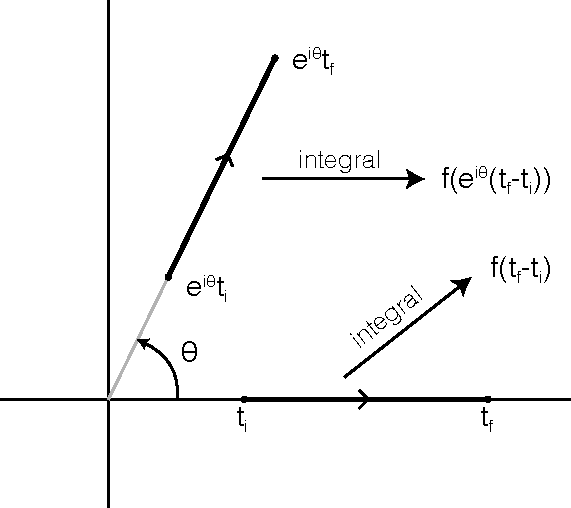
\includegraphics[width=0.5\textwidth]{resources/chap_path_int/wickrot.pdf}
		\caption{An illustration of Wick's rotation.}
		\label{fig:wickrot} 
	\end{figure}
	
	Suppose that 
	\begin{equation}
		L(x,\partial_t x,t)=\frac 12 m (\partial_t x)^t-U(x)
	\end{equation}
	
	Let's define
	\begin{equation}
		L_E(x,\partial_t x,\tau)=-L(x,i\partial_t x,-i\tau)=\frac 12 m (\partial_t x)^2+U(x)
	\end{equation}
	
	Then
	\begin{equation}
		K_E(j,i,t_j-t_i)=C\int \mathcal Dxe^{-\int_{t_i}^{t_j}d\tau L_E(x,\partial_\tau x,\tau)}
	\end{equation}
	
	Note that $L_E$ is the lagragian with potential $-U(x)$.
	\section{Instanton Gas}
	
	The simplest model which exhibit the instanton gas is a particle in double well potential. An example of double well potential is $V(x)=(x^2-a^2)^2$, whose shape is shown in Fig. \ref{fig:dblwell}. Classically, an unmoved particle start at $x=-a$ or $x=a$ would stay at $x=-a$ or $x=a$ forever. In quantum mechanics, the particle oscillates between $x=-a$ and $x=a$.
	\begin{figure}[htb!]
		\centering  
		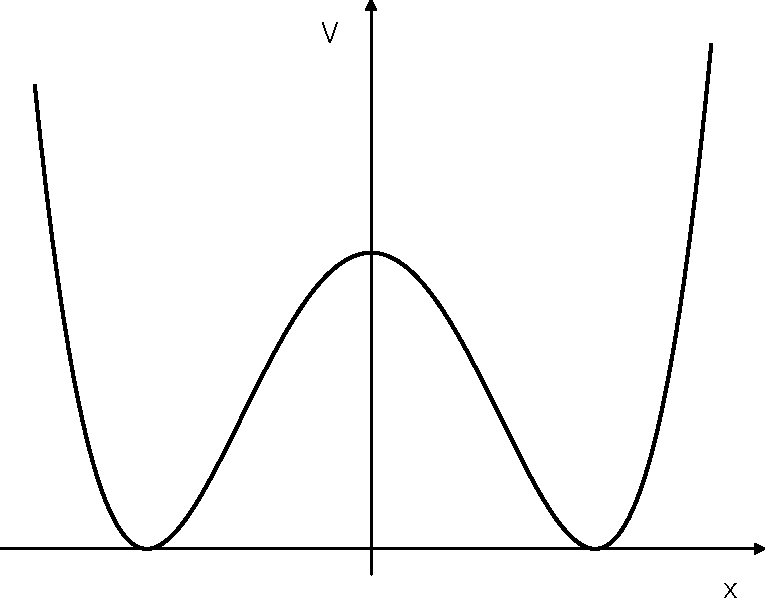
\includegraphics[width=0.5\textwidth]{resources/chap_path_int/doublewell.pdf}
		\caption{A double well potential $V(x)=(x^2-a^2)^2$.}
		\label{fig:dblwell} 
	\end{figure}
	
	We would like to calculate
	\begin{equation}
		K(a,\pm a,t)=\langle \pm a|U(0\rightarrow t)|a\rangle
	\end{equation}
	which is very difficult.
	
	However, we can calculate
	\begin{equation}
		K_E(a,\pm a,t)=C\int \mathcal Dxe^{-\int_{0}^{t}d\tau L_E(x,\partial_\tau x,\tau)}
	\end{equation}
	instead, and get $K(a,\pm a,t)$ by analytic continuation.
	
	For $L_E$, the potential is $-V(x)$, as shown in Fig. \ref{fig:invdblwell}. This is a single well around $x=0$.
	\begin{figure}[htb!]
		\centering  
		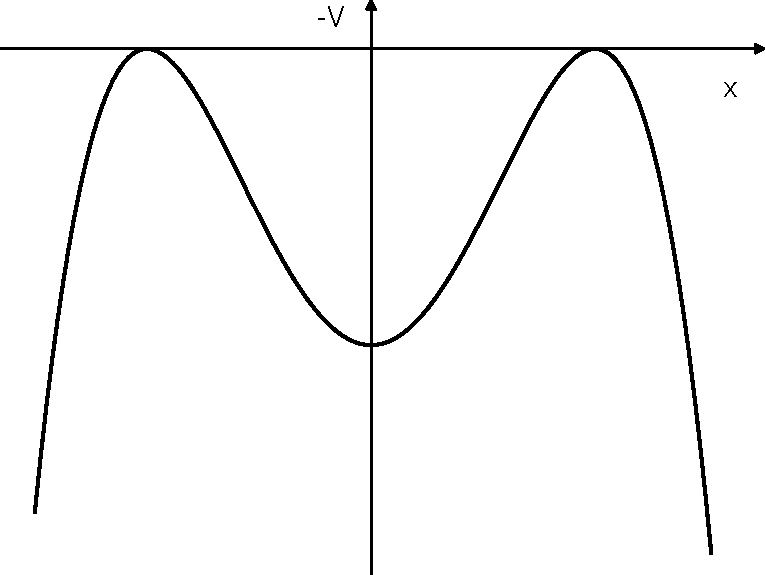
\includegraphics[width=0.5\textwidth]{resources/chap_path_int/invdoublewell.pdf}
		\caption{The potential $-V(x)=-(x^2-a^2)^2$.}
		\label{fig:invdblwell} 
	\end{figure}
	
	As for the imaginary path integral, we can do stationary phase approximation on Euclidian phase integral
	\begin{equation}
		C\int \mathcal Dxe^{-S_E[x]}\simeq C(2\pi)^{N/2}\det(\frac{\delta^2 S}{\delta x\delta x'})^{-1/2}e^{-S_E[x_{cl}]}
	\end{equation}
	
	Let's consider the Euclidian phase integral relative to 2 different classical path
	\begin{enumerate}
		\item As $\tau$ goes from $0\rightarrow T$, $x$ stays at $\pm a$. The Euclidian phase integral is
			\begin{equation}
				\sqrt{\frac{m\omega}{2\pi \sinh(\omega T)}}\sim e^{-\omega T/2}
			\end{equation}
			
			Note that $T$ here is arbitrary, where $\omega$ is the frequency of the harmonic oscillator near $x=\pm a$.
		\item As $\tau$ goes from $0\rightarrow T$, $x$ goes from $\pm a$ to $\mp a$, with energy $E=0$. The Euclidian phase integral is
			\begin{equation}
				Ke^{-S_E[x_{cl}]}
			\end{equation}
			The energy conservation equation is
			\begin{equation}
				\frac 12 m(\partial_\tau x)^2-V(x)=0
			\end{equation}
			
			Then
			\begin{equation}
				S_{inst}=\int_0^Td\tau (\frac 12 m(\partial_\tau x)^2+V(x))=\int_0^Td\tau m(\partial_\tau x)^2=\int_{-a}^a dx m\partial_\tau x=\int_{-a}^a dx \sqrt{2mV(x)}
			\end{equation}
			
			Note that $T\sim \omega_2^{-1}$ here is fixed, where $\omega_2$ is the frequency of the harmonic oscillator near $x=0$.
	\end{enumerate}s
	
	Then a stationary path from $(0,-a)$ to $(T,a)$ is: 
	\begin{enumerate}
		\item Stay at $-a$ for time $t_1$.
		\item Tunnel from $-a$ to $a$.
		\item Stay at $a$ for time $t_2$.
		\item Tunnel from $a$ to $-a$.
		\item Stay at $-a$ for time $t_3$.
		\item \dots\dots
	\end{enumerate}
	This is shown in Fig. \ref{fig:dblwell_path} 
	
	\begin{figure}[htb!]
		\centering  
		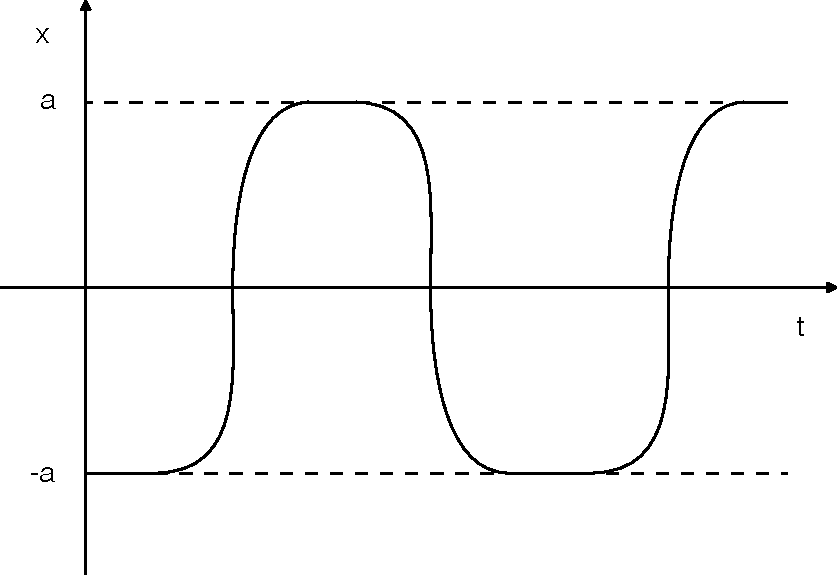
\includegraphics[width=0.6\textwidth]{resources/chap_path_int/dbw_path.pdf}
		\caption{A stationary path for double-well potential}
		\label{fig:dblwell_path} 
	\end{figure}
	
	Assume that $\omega_2^{-1}<< T$, then the path integral contribution of the unmoving part is
	\begin{equation}
		\sim e^{-\omega T/2}
	\end{equation}
	
	The path integral contribution of the tunneling part is
	\begin{equation}
		Ke^{-S_{inst}}
	\end{equation}
	
	So the path integral is 
	\begin{equation}
		K_E(a,-a,T)\sim e^{-\omega T/2}\Big(Ke^{-S_{inst}}\Big)^n
	\end{equation}
	where $n$ is the number of the tunneling process, and $n$ is odd.
	
	However, we should sum up over all possible stationary path: over all odd $n$ and all possible time of the tunneling processes. So
	
	
	\begin{eqnarray}
		K_E(a,-a,T)&\sim& \sum_{n,odd}e^{-\omega T/2}\frac 1{n!}\Big(\prod_i\int_0^T d\tau_i Ke^{-S_{inst}}\Big)\\
		&=&e^{-\omega T/2}\sum_{n,odd}\frac 1{n!}\Big(TKe^{-S_{inst}}\Big)^n\\
		&=&e^{-\omega T/2}\sinh\big(TKe^{-S_{inst}}\big)
	\end{eqnarray}
	
	Similarly
	\begin{equation}
		K_E(a,a,T)\sim e^{-\omega T/2}\cosh\big(TKe^{-S_{inst}}\big)
	\end{equation}
	
	Then
	\begin{eqnarray}
		K(a,-a,t)&\sim&e^{-i\omega t/2}\sin\big(Ke^{-S_{inst}}t\big)\\
		K(a,a,t)&\sim& e^{-i\omega t/2}\cos\big(Ke^{-S_{inst}}t\big)
	\end{eqnarray}
	
	Later we'll show that $K$ is real.
	\section{Fate of the False Vacuum}
	
	A model that exhibits the fate of the false vacuum is a particle in the potential whose shape is shown in Fig. \ref{fig:metastable}. Classically, an unmoved particle start at $x=-a$ would stay at $x=-a$ forever. In quantum mechanics, the particle decay slowly from $x=-a$ to $x=+\infty$. The position $x=-a$ is called the false vacuum.
	\begin{figure}[htb!]
		\centering  
		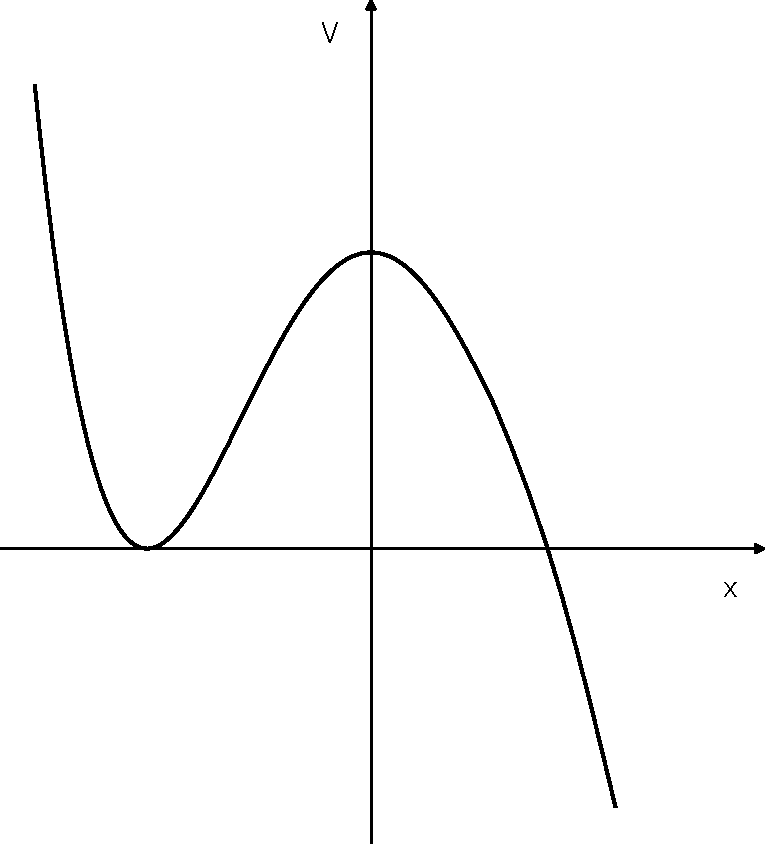
\includegraphics[width=0.5\textwidth]{resources/chap_path_int/metastable.pdf}
		\caption{A potential with a meta-stable state.}
		\label{fig:metastable} 
	\end{figure}
	
	We would like to calculate
	\begin{equation}
		K(-a,-a,t)=\langle \pm a|U(0\rightarrow t)|a\rangle
	\end{equation}
	
	Similarly to the discussion in the last section, we calculate the Euclidean path integral
	\begin{equation}
		K_E(-a,-a,t)=C\int \mathcal Dxe^{-\int_{0}^{t}d\tau L_E(x,\partial_\tau x,\tau)}
	\end{equation}
	whose potential is shown in Fig. \ref{fig:invmetastable}.
	\begin{figure}[htb!]
		\centering  
		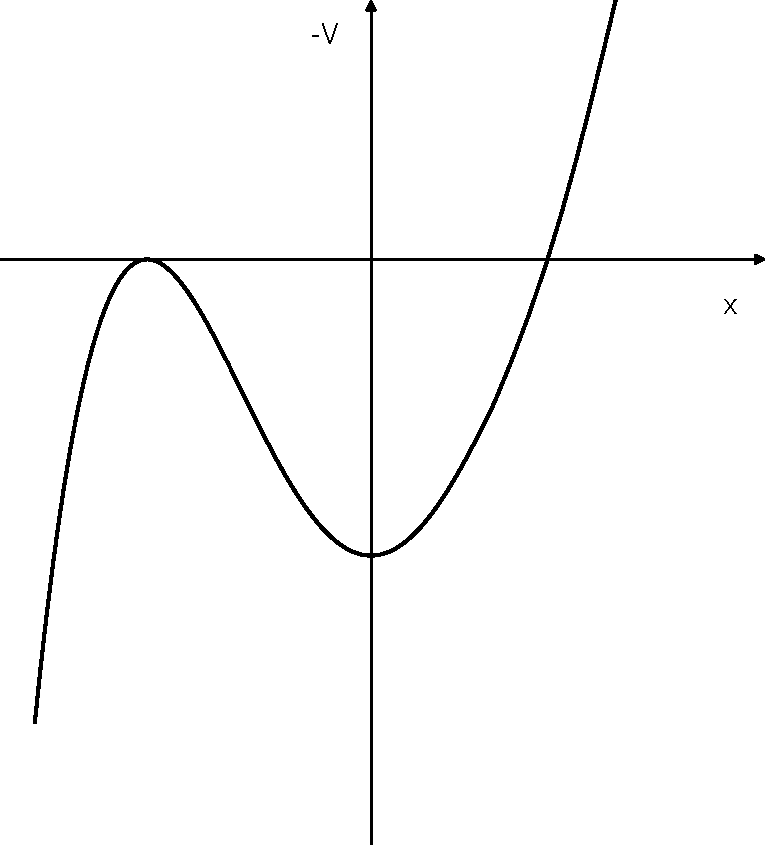
\includegraphics[width=0.5\textwidth]{resources/chap_path_int/invmetastable.pdf}
		\caption{The inverse of the potential with a meta-stable state.}
		\label{fig:invmetastable} 
	\end{figure}
	
	Similarly, there're two types of typical classical path
	\begin{enumerate}
		\item As $\tau$ goes from $0\rightarrow T$, $x$ stays at $-a$. The Euclidian phase integral is
			\begin{equation}
				\sqrt{\frac{m\omega}{2\pi \sinh(\omega T)}}\sim e^{-\omega T/2}
			\end{equation}
			
		\item As $\tau$ goes from $0\rightarrow T$, $x$ goes from $-a$ to $b$ ($V(b)=0$) then back to $-a$, with energy $E=0$. The Euclidian phase integral is
			\begin{equation}
				Ke^{-S_{bounce}}
			\end{equation}
	\end{enumerate}
	
	Then a stationary path from $(0,-a)$ to $(T,-a)$ is: 
	\begin{enumerate}
		\item Stay at $-a$ for time $t_1$.
		\item Bounce from $-a$ to $b$ then back to $-a$.
		\item Stay at $-a$ for time $t_2$.
		\item Bounce from $-a$ to $b$ then back to $-a$.
		\item Stay at $-a$ for time $t_3$.
		\item \dots\dots
	\end{enumerate}
	This is shown in Fig. \ref{fig:meta_path} 
	
	\begin{figure}[htb!]
		\centering  
		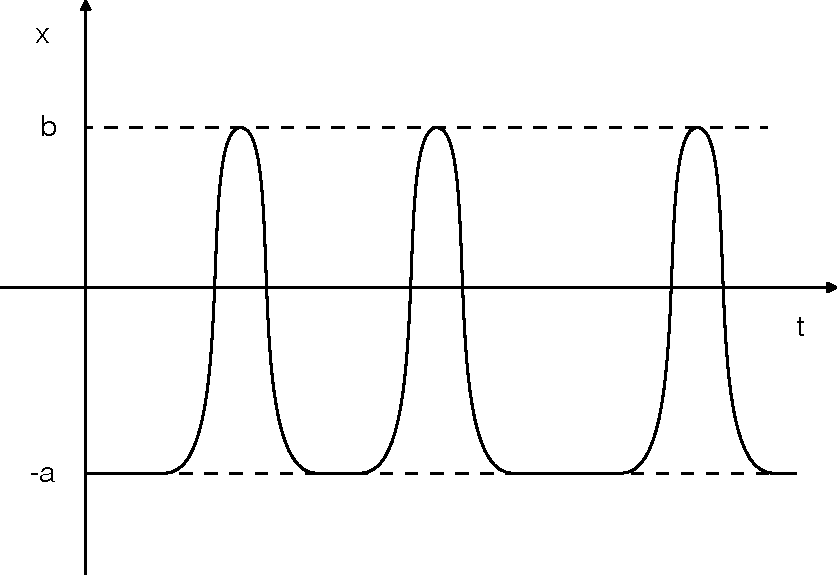
\includegraphics[width=0.6\textwidth]{resources/chap_path_int/meta_path.pdf}
		\caption{A stationary path for meta-stable potential}
		\label{fig:meta_path} 
	\end{figure}

	Similar to the double-well potential case, the Euclidean path integral is
	\begin{equation}
		K_E(-a,-a,T)\sim \sum_{n}e^{-\omega T/2}\frac 1{n!}\Big(\prod_i\int_0^T d\tau_i Ke^{-S_{bounce}}\Big)=e^{-\omega T/2}e^{TKe^{-S_{bounce}}}
	\end{equation}
	
	Then
	\begin{equation}
		K(-a,-a,t)\sim e^{-i\omega t/2}e^{-|K|e^{-S_{bounce}}t}
	\end{equation}
	Later we'll show that $K$ is imaginary.
	
	\section{Is $K$ Real or Imaginary?}
	
	\begin{equation}
		S_E[x]\simeq S_E[x_{cl,\tau}]+\frac 12\int_{t_i}^{t_j}d\tau \delta x(- m\partial_\tau^2+V(x_{cl,\tau})'')\delta x
	\end{equation}
	where $x_{cl,\tau}$ is the instaton or the bounce process at $\tau$.
	
	Then
	\begin{equation}
		K\sim det(-m\partial_\tau^2+V(x_{cl,\tau})'')^{-1/2}
	\end{equation}
	
	However, the classical contribution is integrated over $\tau$, so in $det(-m\partial_\tau^2+V(x_{cl,\tau})'')$, one should only consider the $\delta x$ perpendicular to $\partial_\tau x_{cl,\tau}$. 
	
	It can be shown that 
	\begin{equation}
		(-m\partial_\tau^2+V(x_{cl,\tau})'')\partial_\tau x_{cl,\tau}=0
	\end{equation}
	and the operator $-m\partial_\tau^2+V(x_{cl,\tau})''$ is non-degenerate.
	
	So
	\begin{equation}
		K\sim det'(-m\partial_\tau^2+V(x_{cl,\tau})'')^{-1/2}
	\end{equation}
	where the zero eigenvalue is omitted.
	
	If the potential is double-well, $\partial_\tau x_{cl,\tau}$ has no node, so $-m\partial_\tau^2+V(x_{cl,\tau})''$ has no negative eigenvalue. So $det(-m\partial_\tau^2+V(x_{cl,\tau})'')>0$ and $K$ is real.
	
	If the potential is of the shape in Fig. \ref{fig:metastable}, $\partial_\tau x_{cl,\tau}$ has a node, so $-m\partial_\tau^2+V(x_{cl,\tau})''$ has a negative eigenvalue. So $det(-m\partial_\tau^2+V(x_{cl,\tau})'')<0$ and $K$ is imaginary.
	
	\section{Path Integral for Spin}
	
	Let
	\begin{equation}
		H=B\cdot \hat S
	\end{equation}
	
	We have
	\begin{eqnarray}
		\langle g'|U(t\rightarrow t+\Delta t)|g\rangle&=&\langle g'|e^{-i\Delta tH}|g\rangle\\
		&=&\langle g'|g\rangle-i\Delta t\langle g'|H|g\rangle+\mathcal O(\Delta t^2)\\
		&=&e^{\ln \langle g'|g\rangle-i\Delta t\frac{\langle g'|H|g\rangle}{\langle g'|g\rangle}}\\
		&=&e^{S\ln[(1+n_{g'}\cdot n_g)/2]+iS(\Delta\chi+\Phi(\vec z,n_g,n_{g'}))-i\Delta t\frac{\langle g'|H|g\rangle}{\langle g'|g\rangle}}
	\end{eqnarray}
	
	Let's consider mild oscillating trajectories, that is, $\Delta g\sim \Delta t$. Then
	\begin{equation}
		\langle g'|U(t\rightarrow t+\Delta t)|g\rangle=e^{-\frac 14S (\Delta n_g)^2+iS(\Delta\chi+\Phi(\vec z,n_g,n_{g'}))-i\Delta tB\cdot n_g}
	\end{equation}
	
	So
	\begin{eqnarray}
		\langle g_f|U(t_i\rightarrow t_f)|g_i\rangle
		&=&\int \mathcal D g e^{iS_{WZ}+i\int_{t_i}^{t_f}dt(\frac i4S\Delta t (\dot n_g)^2+S\dot\chi-B\cdot n_g}\\
		&=&e^{iS(\chi_f-\chi_i)}\int \mathcal D n_g e^{iS_{WZ}+i\int_{t_i}^{t_f}dt(i\epsilon (\dot n_g)^2-B\cdot n_g)}
	\end{eqnarray}
	where $\mathcal D g$ is integrated over $d\theta d\phi d\chi$ and $\mathcal D n_g$ is integrated over $d\theta d\phi $, and $S_{WZ}$ is $S$ times the area enclosed by the path $\gamma:\vec z\rightarrow n_{g_i}\overset{n_{g(t)}}{\longrightarrow} n_{g_f}\rightarrow\vec z$.
	
	Let $A=\frac{1-\cos\theta}{\sin\theta}\hat e_{\phi}$, then $B'=\nabla\times A=\hat e_r$. So
	\begin{equation}
		S_{WZ}=S\int dS\cdot \hat e_r=S\int dS\cdot(\nabla\times A)=S\int _\gamma dn\cdot A
	\end{equation}
	
	Then
	\begin{equation}
		\langle g_f|U(t_i\rightarrow t_f)|g_i\rangle=e^{iS(\chi_f-\chi_i)}\int \mathcal D n_g e^{i\int_{t_i}^{t_f}dt(S\dot n_g\cdot A+i\epsilon (\dot n_g)^2-B\cdot n_g)}
	\end{equation}
	since $dn\cdot A=0$ along a meridian. 
	
	
	\chapter{Second Quantization}
	
	In this chapter, we discuss the quantum mechanics many-particle situation. We'll show how the states and operators are expressed by creation/annihilation operators.
	\section{Identical Particles}
	
	In a single particle Hilbert space $\mathbb H$, we have orthogonal-normalized basis: $|0\rangle$, $|1\rangle$, $|2\rangle$ ... We can construct a Hilbert space for $N$ particles by tensor product $N$ single particle Hilbert spaces.
	
	We have a basis $|\{\lambda_i\}\rangle=|\lambda_1\lambda_2\dots\lambda_N\rangle$ where $\lambda_i=0,1,\cdots$ denotes the state of $i$th particle. We define the inner product in $\mathbb H^{\otimes N}$ by requiring that $|\{\lambda_i\}\rangle$ form a orthogonal-normalized basis. This definition of inner product of $\mathbb H^{\otimes N}$ is independent of the choice of orthogonal-normalized basis in $\mathbb H$.
	
	
	We define the linear action $P$ of the permutation group $S_N$ on $\mathbb H^{\otimes N}$ by defining that its act on the basis of $\mathbb H^{\otimes N}$ as
	\begin{equation}
		P(g)|\lambda_1\lambda_2\dots\lambda_N\rangle=|\lambda_{g(1)}\lambda_{g(2)}\dots\lambda_{g(N)}\rangle\quad g\in S_N
	\end{equation}
	This definition of action of $S_N$ is also independent of the choice of basis in $\mathbb H$.
	
	
	The principle of quantum mechanics states that particles of the same type are identical and indistinguishable. So if a many-body state lies in $\mathbb H^{\otimes N}$, it must be left invariant under permutation, since nothing has been actually done. It means if $|\Phi\rangle$ is a many-body state,
	\begin{equation}
		P(g)|\Phi\rangle=e^{i\theta}|\Phi\rangle
	\end{equation}
	
	So $|\Phi\rangle$ forms the space for 1-D representation of $S_N$. The only two 1-D representations of $S_N$ are $P(g)=1$ and $P(g)={\rm sgn}(g)$. We define \index{boson}bosons to be particles with wave-function such that $P(g)|\Phi\rangle=|\Phi\rangle$. Such states form a subspace of $\mathbb H^{\otimes N}$ called ${\rm sym}(\mathbb H^{\otimes N})$. And we define \index{fermion}fermions to be particles with wave-function such that $P(g)|\Phi\rangle={\rm sgn}(g)|\Phi\rangle$. Such states form a subspace of $\mathbb H^{\otimes N}$ called ${\rm asm}(\mathbb H^{\otimes N})$.\index{${\rm sym}(\mathbb H^{\otimes N})$, ${\rm asm}(\mathbb H^{\otimes N})$}
	
	Define\index{$S_+$, $S_-$}
	\begin{eqnarray}
		S_+&=&\frac 1{N!}\sum_{g\in S_N}P(g)\\
		S_-&=&\frac 1{N!}\sum_{g\in S_N}P(g){\rm sgn}(g)\\		
	\end{eqnarray}	
	
	It's easy to see that $S_+$ and $S_-$ are orthogonal projective operators:
	\begin{eqnarray}
		S_+S_+&=&S_+\\
		S_-S_-&=&S_-\\
		S_+S_-&=&S_-S_+=0
	\end{eqnarray}
		
	\begin{theorem}
		\begin{eqnarray}
			{\rm sym}(\mathbb H^{\otimes N})&=&S_+\mathbb H^{\otimes N}\\
			{\rm asm}(\mathbb H^{\otimes N})&=&S_-\mathbb H^{\otimes N}
		\end{eqnarray}
	\end{theorem}
	\begin{proof}
		For $|\Phi\rangle\in{\rm sym}(\mathbb H^{\otimes N})$,
		\begin{eqnarray}
			\sum_{g\in S_N}P(g)|\Phi\rangle&=&N!|\Phi\rangle\\
			|\Phi\rangle&=&\frac 1{N!}\sum_{g\in S_N}P(g)|\Phi\rangle\\
			&=&S_+|\Phi\rangle	
		\end{eqnarray}
		
		For $|\Phi\rangle\in{\rm asm}(\mathbb H^{\otimes N})$,
		\begin{eqnarray}
			\sum_{g\in S_N}{\rm sgn}(g)P(g)|\Phi\rangle&=&N!|\Phi\rangle\\
			|\Phi\rangle&=&\frac 1{N!}\sum_{g\in S_N}{\rm sgn}(g)P(g)|\Phi\rangle\\
			&=&S_-|\Phi\rangle		
		\end{eqnarray}
		
		Thus
		\begin{eqnarray}
			{\rm sym}(\mathbb H^{\otimes N})&=&S_+{\rm sym}(\mathbb H^{\otimes N})\subset S_+\mathbb H^{\otimes N}\\
			{\rm asm}(\mathbb H^{\otimes N})&=&S_-{\rm asm}(\mathbb H^{\otimes N})\subset S_-\mathbb H^{\otimes N}
		\end{eqnarray}
		
		It's easy to check that
		\begin{eqnarray}
			P(g)S_+&=&S_+P(g)=S_+\\
			P(g)S_-&=&S_-P(g)={\rm sgn}(g)S_-
		\end{eqnarray}
		
		Thus for any $|\Psi\rangle$, $S_\pm|\Psi\rangle\in{\rm sym}(\mathbb H^{\otimes N})/{\rm asm}(\mathbb H^{\otimes N})$.
		
		Thus
		\begin{eqnarray}
			S_+(\mathbb H^{\otimes N})&\subset&{\rm sym}(\mathbb H^{\otimes N})\\
			S_-(\mathbb H^{\otimes N})&\subset&{\rm asm}(\mathbb H^{\otimes N})
		\end{eqnarray}
	\end{proof}
	
	Thus the basis for the space ${\rm sym}(\mathbb H^{\otimes N})/{\rm asm}(\mathbb H^{\otimes N})$ is $S_\pm|\{\lambda_i\}\rangle$.
	
	For boson, it can be easily shown that
	\begin{eqnarray}
		S_+|\{\lambda_i\}\rangle&\neq&0\\
		\langle\{\lambda_i\}|S_+S_+|\{\lambda_i\}\rangle&=&\langle\{\lambda_i\}|S_+|\{\lambda_i\}\rangle=\frac{\prod_i n_i!}{N!}\\
		S_+|\{\lambda_i\}\rangle&=&S_+|\{\lambda'_i\}\rangle\ {\rm iff}\ \exists g:|\{\lambda_i\}\rangle=P(g)|\{\lambda'_i\}\rangle\\
		S_+|\{\lambda_i\}\rangle&\perp&S_+|\{\lambda'_i\}\rangle\ {\rm if}\ S_+|\{\lambda_i\}\rangle\neq S_+|\{\lambda'_i\}\rangle	
	\end{eqnarray}
	
	Thus $\sqrt{\frac{N!}{\prod_i n_i!}}S_+|\{\lambda_i\}\rangle$ is a orthogonal basis for ${\rm sym}(\mathbb H^{\otimes N})$, where $n_i$ is the number of particles at $i$th state. And each set of physically equivalent basis vectors in $\mathbb H^{\otimes N}$ give only one basis vector in ${\rm sym}(\mathbb H^{\otimes N})$.	
	
	For fermion, first consider $|\{\lambda_i\}\rangle$ with multiple occupation, that is, $\lambda_i=\lambda_j$ for some $i\neq j$.
	\begin{eqnarray}
		|\{\lambda_i\}\rangle&=&P((i,j))|\{\lambda_i\}\rangle\\
		S_-|\{\lambda_i\}\rangle&=&S_-P((i,j))|\{\lambda_i\}\rangle\\
		S_-|\{\lambda_i\}\rangle&=&-S_-|\{\lambda_i\}\rangle\\
		S_-|\{\lambda_i\}\rangle&=&0
	\end{eqnarray}
	
	For $|\{\lambda_i\}\rangle$ without multiple occupation, it can be easily shown that
	\begin{eqnarray}
		S_-|\{\lambda_i\}\rangle&\neq&0\\
		\langle\{\lambda_i\}|S_-S_-|\{\lambda_i\}\rangle&=&\langle\{\lambda_i\}|S_-|\{\lambda_i\}\rangle=\frac 1{N!}\\
		S_-|\{\lambda_i\}\rangle&=&\pm S_-|\{\lambda'_i\}\rangle\ {\rm iff}\ \exists g:|\{\lambda_i\}\rangle=P(g)|\{\lambda'_i\}\rangle\\
		S_-|\{\lambda_i\}\rangle&\perp&S_-|\{\lambda'_i\}\rangle\ {\rm if}\ S_-|\{\lambda_i\}\rangle\neq\pm S_-|\{\lambda'_i\}\rangle	
	\end{eqnarray}
	
	Thus $\sqrt{N!}S_-|\{\lambda_i\}\rangle$ is a normalized-orthogonal basis for ${\rm asm}(\mathbb H^{\otimes N})$, and we can still express it as $\sqrt{\frac{N!}{\prod_i n_i!}}S_+|\{\lambda_i\}\rangle$ as in the boson case.
	
	To describe a system with variable particle numbers, we define the \index{Fock space}\textbf{Fock space} for boson as
	\begin{equation}
		\bigoplus_{N=0}^\infty{\rm sym}(\mathbb H^{\otimes N})
	\end{equation}
	and for fermion as
	\begin{equation}
		\bigoplus_{N=0}^\infty{\rm asm}(\mathbb H^{\otimes N})
	\end{equation}
	where ${\rm sym}(\mathbb H^{\otimes 0})={\rm asm}(\mathbb H^{\otimes 0})=(|vac\rangle)$ is a 1-D space spanned by the \index{vacuum state}vacuum state, which stands for the state with no particles.
	
	It's convenient to express the basis of Fock space in \index{particle number representation}\textbf{particle number representation}. That is, define
	\begin{equation}
		|n_0n_1...\rangle=\sqrt{\frac{N!}{\prod_i n_i!}}S_\pm|\{\lambda_i\}\rangle
	\end{equation}
	where $n_i$ is the number of particles with $i$th state in $|\{\lambda_i\}\rangle$. It's easy to see, this definition has an ambiguity of $\pm1$ for fermion. Thus to eliminate this ambiguity, we require that the $|\{\lambda_i\}\rangle$ in the definition to be of increasing order, that is, $\lambda_1\leq\lambda_2\leq\cdots$. With this definition, it's easy to see $|n_0n_1\dots\rangle$ is different for different $\{n_i\}$ and forms a orthogonal-normalized basis of the Fock space, and we call it \textbf{particle number basis}. Especially, we express $|vac\rangle$ as $|0\cdots\rangle$ or $|0\rangle$.
	\section{Creation \& Annihilation Operators}
	We can define the \textbf{creation} and \textbf{annihilation operators} to simplify operators in Fock space.
	
	The \index{creation operator}creation operator in defined as
	\begin{equation}
		a_i^\dagger|n_0n_1\dots n_i\dots\rangle=\sqrt{n_i+1}\xi^{\sum_{j<i}n_i}|n_0n_1\dots n_i+1\dots\rangle
	\end{equation}
	where $\xi=\pm1$ for boson/fermion.
	
	Then we have 
	\begin{equation}
		|n_0n_1\dots\rangle=\frac{(a_0^\dagger)^{n_0}}{\sqrt{n_0!}}\frac{(a_1^\dagger)^{n_1}}{\sqrt{n_1!}}\cdots|0\rangle
	\end{equation}
	
	The \index{annihilation operator}annihilation operator is defined as the conjugation of the creation operator. We have
	\begin{equation}
		a_i|n_0n_1\dots n_i\dots\rangle=\left\{\begin{array}{cc}
		\sqrt{n_i}\xi^{\sum_{j<i}n_i}|n_0n_1\dots n_i-1\dots\rangle&(n_i>0)\\
		0&(n_i=0)\\
		\end{array}\right.
	\end{equation}
	
	Physically, $a_i^\dagger/a_i$ means to add/remove a particle of the $i$th state.
	
	We have the following \index{commuting/anti-commuting relations}\textbf{commuting/anti-commuting relations}
	\begin{equation}
		[a_i,a_i]_\xi=[a_i^\dagger,a_i^\dagger]_\xi=0,\ [a_i,a_i^\dagger]_\xi=\delta_{ij}
	\end{equation}
	where $\xi=\pm$ for boson/fermion.
	
	We prove the following lemma
	\begin{lemma}\label{lem:aS}
		\begin{equation}
			a_\lambda^\dagger S_\pm|\lambda_1\lambda_2\dots\rangle=\sqrt{N+1}S_\pm|\lambda\lambda_1\lambda_2\dots\rangle
		\end{equation}
	\end{lemma}
	\begin{proof}
		For boson
		\begin{eqnarray}
			a_\lambda^\dagger S_+|\lambda_1\lambda_2\dots\rangle&=&a_\lambda^\dagger S_+|\lambda_{g(1)}\lambda_{g(2)}\dots\rangle\\
			&=&a_\lambda^\dagger\sqrt{\frac{\prod_i n_i!}{N!}}|n_1n_2\dots\rangle\\
			&=&\sqrt{n_\lambda+1}\sqrt{\frac{\prod_i n_i!}{N!}}|n_1n_2\dots n_\lambda+1\dots\rangle\\
			&=&\sqrt{N+1}S_+|\lambda_{g(1)}\lambda_{g(2)}\dots\lambda\dots\rangle\\
			&=&\sqrt{N+1}S_+|\lambda\lambda_1\lambda_2\dots\rangle
		\end{eqnarray}
		where $\lambda_{g(1)}\leq\lambda_{g(2)}\leq\cdots$.
		
		For fermion
		\begin{eqnarray}
			a_\lambda^\dagger S_-|\lambda_1\lambda_2\dots\rangle&=&a_\lambda^\dagger{\rm sgn}(g)S_-|\lambda_{g(1)}\lambda_{g(2)}\dots\rangle\\
			&=&a_\lambda^\dagger{\rm sgn}(g)\sqrt{\frac{\prod_i n_i!}{N!}}|n_1n_2\dots\rangle\\
			&=&(-1)^{\sum_{\lambda'<\lambda}n_{\lambda'}}\sqrt{n_\lambda+1}{\rm sgn}(g)\sqrt{\frac{\prod_i n_i!}{N!}}|n_1n_2\dots n_\lambda+1\dots\rangle\\
			&=&(-1)^{\sum_{\lambda'<\lambda}n_{\lambda'}}{\rm sgn}(g)\sqrt{N+1}S_-|\lambda_{g(1)}\lambda_{g(2)}\dots\lambda\dots\rangle\\
			&=&{\rm sgn}(g)\sqrt{N+1}S_-|\lambda\lambda_{g(1)}\lambda_{g(2)}\dots\rangle\\
			&=&\sqrt{N+1}S_-|\lambda\lambda_1\lambda_2\dots\rangle
		\end{eqnarray}
		where similarly, $\lambda_{g(1)}\leq\lambda_{g(2)}\leq\cdots$.
	\end{proof}
	
	Sometimes we may want to change the basis of the single particle Hilbert space $\mathbb H$. Suppose $|\mu\rangle$s and $|\nu\rangle$s are two set of orthogonal-normalized basis. It would be nice if we can relate $a_\lambda/a_\lambda^\dagger$ with $a_\mu/a_\mu^\dagger$. Since $S_\pm$ is independent of the basis of $\mathbb H$, ${\rm sym}(\mathbb H^{\otimes N})/{\rm asm}(\mathbb H^{\otimes N})$ are the same for two basis. Thus Fock space for two basis are the same. Using the Lemma \ref{lem:aS}, we can prove the following theorem
	\begin{theorem}
		\begin{equation}
			a_\mu^\dagger=a_\lambda^\dagger\langle\lambda|\mu\rangle
		\end{equation}
	\end{theorem}
	\begin{proof}
		Since the Fock space for two basis are the same, $a_\lambda^\dagger$ and $a_\mu^\dagger$ live in the same space. We only need to prove that their actions on a set of basis vectors are the same. That is, we only need to prove
		\begin{equation}
			a_\mu^\dagger|n_\mu\rangle=a_\lambda^\dagger\langle\lambda|\mu\rangle|n_\mu\rangle
		\end{equation}
		
		Suppose $N=\sum n_\mu$,
		\begin{eqnarray}
			{\rm RHS}&=&a_\lambda^\dagger\langle\lambda|\mu\rangle\sqrt{\frac{N!}{\prod_i n_i!}}S_\pm|\mu_1\dots\mu_N\rangle\quad(\mu_1\leq\cdots\leq\mu_N)\\
			&=&a_\lambda^\dagger\langle\lambda|\mu\rangle\sqrt{\frac{N!}{\prod_i n_i!}}S_\pm\langle\lambda_1|\mu_1\rangle\cdots\langle\lambda_N|\mu_N\rangle|\lambda_1\dots\lambda_N\rangle\\
			&=&\sqrt{\frac{(N+1)!}{\prod_i n_i!}}S_\pm\langle\lambda|\mu\rangle\langle\lambda_1|\mu_1\rangle\cdots\langle\lambda_N|\mu_N\rangle|\lambda\lambda_1\dots\lambda_N\rangle\\
			&=&\sqrt{\frac{(N+1)!}{\prod_i n_i!}}S_\pm|\mu\mu_1\dots\mu_N\rangle\\
			&=&\xi^{\sum_{\mu'<\mu}n_{\mu'}}\sqrt{\frac{(N+1)!}{\prod_i n_i!}}S_\pm|\mu_1\dots\mu\dots\mu_N\rangle\\
			&=&\sqrt{n_\mu+1}\xi^{\sum_{\mu'<\mu}n_{\mu'}}|n_1\dots n_\mu+1\dots\rangle\\
			&=&{\rm LHS}
		\end{eqnarray}
	\end{proof}
	And obviously we have
	\begin{equation}
		a_\mu=a_\lambda\langle\mu|\lambda\rangle
	\end{equation}
	\section{Second Quantization of Operators}
	For a one-body operator $O$ in $\mathbb H$ defined by
	\begin{equation}
		O=O_{\mu\nu}|\mu\rangle\langle\nu|
	\end{equation}
	
	Then the total $O$ operator in $\mathbb H^{\otimes N}$ is
	\begin{equation}
		O_N=\sum_{i=1}^NO_{\mu\nu}|\mu_i\rangle\langle\nu_i|
	\end{equation}
	where $|\mu_i\rangle\langle\nu_i|$ is short for
	\begin{equation}
		\prod_{j=1}^{i-1}id\otimes|\mu\rangle\langle\nu|\otimes\prod_{j=i+1}^{N}id
	\end{equation}
	
	$O_N$ is symmetric in the sense that
	\begin{eqnarray}
		P(g)O_NP(g^{-1})&=&\sum_{i=1}^NO_{\mu\nu}P(g)|\mu_i\rangle\langle\nu_i|P(g^{-1})\\
		&=&\sum_{i=1}^NO_{\mu\nu}|\mu_{g(i)}\rangle\langle\nu_{g(i)}|\\
		&=&\sum_{i=1}^NO_{\mu\nu}|\mu_i\rangle\langle\nu_i|\\
		&=&O_N
	\end{eqnarray}
	
	Thus
	\begin{equation}
		S_\pm O_N=O_NS_\pm
	\end{equation}
	
	Thus
	\begin{equation}
		O_N{\rm sym}/{\rm asm}(\mathbb H^{\otimes N})=O_NS_\pm\mathbb H^{\otimes N}=S_\pm O_N\mathbb H^{\otimes N}\subset S_\pm\mathbb H^{\otimes N}={\rm sym}/{\rm asm}(\mathbb H^{\otimes N})
	\end{equation}
	that is, ${\rm sym}(\mathbb H^{\otimes N})/{\rm asm}(\mathbb H^{\otimes N})$ are invariant spaces of $O_N$.
	
	We can defined an operator $O$ in the Fock space which acts on N particle states like $O_N$. Then
	\begin{eqnarray}
		O|n_\lambda\rangle&=&O_N|n_\lambda\rangle\quad (N=\sum n_\lambda)\\
		&=&O_NS_\pm\sqrt{\frac{N!}{\prod n_\lambda!}}|\lambda_1\dots\lambda_N\rangle\quad (\lambda_1\leq\cdots\leq\lambda_N)\\
		&=&S_\pm\sqrt{\frac{N!}{\prod n_\lambda!}}O_N|\lambda_1\dots\lambda_N\rangle\\
		&=&S_\pm\sqrt{\frac{N!}{\prod n_\lambda!}}\sum_{i=1}^NO_{\lambda'_i\lambda_i}|\lambda_1\dots\lambda'_i\dots\lambda_N\rangle\\
		&=&\sum_{i=1}^N\sum_{\lambda'_i\neq\lambda_i}\sqrt{\frac{n_{\lambda'_i}+1}{n_{\lambda_i}}}O_{\lambda'_i\lambda_i}\xi^{n(\lambda_i,\lambda'_i)}|n_1\dots n_{\lambda'_i}+1\dots n_{\lambda_i}-1\dots\rangle+\nonumber\\
		&&\sum_{i=1}^NO_{\lambda_i\lambda_i}|n_1\dots \rangle\\
		&=&\sum_{n_\lambda>0}\sum_{\lambda'\neq\lambda}\sqrt{n_{\lambda'}+1}\sqrt{n_\lambda}O_{\lambda'\lambda}\xi^{n(\lambda,\lambda')}|n_1\dots n_{\lambda'}+1\dots n_\lambda-1\dots\rangle+\nonumber\\
		&&\sum_{n_\lambda>0}n_\lambda O_{\lambda\lambda}|n_1\dots \rangle
	\end{eqnarray}
	where $n(\lambda,\lambda')$ is the number of particles with states that lie strictly between $\lambda$ and $\lambda'$.
	
	We have
	\begin{equation}
		a_{\lambda'}^\dagger a_\lambda|n_\lambda\rangle=\sqrt{n_{\lambda'}+1}\sqrt{n_\lambda}\xi^{n(\lambda,\lambda')}|n_1\dots n_{\lambda'}+1\dots n_\lambda-1\dots\rangle\quad(n_\lambda>0,\lambda'\neq\lambda)
	\end{equation}
	
	Thus
	\begin{equation}
		O|n_\lambda\rangle=O_{\lambda'\lambda} a_{\lambda'}^\dagger a_\lambda|n_\lambda\rangle
	\end{equation}
	
	Since this equation holds for all $|n_\lambda\rangle$, we finally get
	\begin{equation}
		O=O_{\mu\nu}a_\mu^\dagger a_\nu
	\end{equation}
	
	For a two-body operator in $\mathbb H^{\otimes N}$
	\begin{equation}
		O_N=\frac 12\sum_{i\neq j}O_{\alpha\beta\mu\nu}|\alpha_i\beta_j\rangle\langle\mu_i\nu_j|
	\end{equation}
	
	We can define the operator $O$ in the Fock space in the same manner, and similarly
	\begin{equation}
		O=\frac 12O_{\alpha\beta\mu\nu}a_{\alpha}^\dagger a_{\beta}^\dagger a_\nu a_\mu
	\end{equation}
	\paragraph{Example}
	For a free Hamiltonian with only one-body term $T_{\mu\nu}|\mu\rangle\langle\nu|$, its second-quantized form is
	\begin{equation}
		H=T_{\mu\nu} a_\mu^\dagger a_\nu
	\end{equation}
	To diagonal a second quantized free Hamiltonian means to find $a_i$ such that
	\begin{equation}
		H=E_in_i
	\end{equation}
	
	Suppose we can diagonalize the $H$ matrix by a unitary matrix $U$ 
	\begin{equation}
		UTU^{-1}=T'={\rm diag}(E_1,E_2,\dots)
	\end{equation}
	
	Define $\tilde{a}$ to be 
	\begin{equation}
		\tilde{a}_\mu=U_{\mu\nu}a_\nu
	\end{equation}
	
	Then
	\begin{equation}
		H=T'_{\mu\nu} \tilde{a}_\mu^\dagger \tilde{a}_\nu=E_\mu \tilde{n}_\mu
	\end{equation}
	
	Clearly $H$ is diagonal over the particle number basis of $\tilde{a}/\tilde{a}^\dagger$.
	
	For a Hamiltonian with two-body interaction, it's general form is 
	\begin{equation}
		H=T_{\mu\nu} a_\mu^\dagger a_\nu+\frac 12U_{\alpha\beta\mu\nu}a_{\alpha}^\dagger a_{\beta}^\dagger a_\nu a_\mu
	\end{equation}
	
	There's in general no easy way to diagonalize this many-body Hamiltonian strictly rather than the exact diagonalization method. But its ground state can be more easily derived approximately by the \index{Hatree-Fock method}\textbf{Hatree-Fock method}. For N electrons, the ground state is obtained by minimizing the total energy of the state of the form
	\begin{equation}
		\prod_i\Big(\sum_\mu c_{i\mu}a_\mu^\dagger\Big)|0\rangle
	\end{equation}
	where $c_{i\mu}$s are variational parameters.	
	
\chapter{Green's Function for Many-body System}

\section{Green's Function}
	N-point Green's function is defined by
	\begin{equation}
		G(i_1,t_1,\dots,i_n,t_n)=(-i)\langle \Omega|T[O(i_1,t_1)\cdots O(i_n,t_n)]|\Omega\rangle
	\end{equation}

	The simplest kind of Green's function is the transition amplitude from the ith state to the jth state after time $t$:
	\begin{eqnarray}
		G(j,t_j;i,t_i)&=&(-i)\langle \Omega|T[a_{j}(t_j)a^\dagger_{i}(t_i)]|\Omega\rangle\\
		&=&(-i)e^{iE_0|t_j-t_i|}[\langle j|U(t_i\rightarrow t_j)]|i\rangle\theta(t_j-t_i)+\xi\langle \tilde i|U(t_j\rightarrow t_i)]|\tilde j\rangle\theta(t_i-t_j)]
	\end{eqnarray}
	where $\xi=\pm 1$ for boson/fermion, $|0\rangle$ is the ground state, $a(t)$ is in Heisenberg picture, and $|i\rangle=a^\dagger_i|0\rangle$ and $|\tilde i\rangle=a_i|0\rangle$.
	
	For non-interacting system, $a_i|0\rangle=0$. So
	\begin{equation}
		G(j,t_j;i,t_i)=(-i)e^{iE_0|t_j-t_i|}\langle j|U(t_i\rightarrow t_j)]|i\rangle\theta(t_j-t_i)
	\end{equation}
	which returns to the old result.
	
\section{Propagator of Free System}

	A propagator is a two-point Green's function with field operators.
	\subsection{Free Fermions}
	The Hamiltonian reads
	\begin{equation}
		H=\sum_{k\sigma}\epsilon_k c_{k\sigma}^\dagger c_{k\sigma}-\mu N=\sum_{k\sigma}\tilde\epsilon_k c_{k\sigma}^\dagger c_{k\sigma}
	\end{equation}
	where $\tilde\epsilon_k=\epsilon_k-\mu$
	
	We have
	\begin{equation}
		|\Omega\rangle=\prod_{\tilde\epsilon_k<0,\sigma}c_{k\sigma}^\dagger|0\rangle
	\end{equation}
	and
	\begin{equation}
		c_{k\sigma}(t)=e^{-i\tilde\epsilon_kt}c_{k\sigma}
	\end{equation}
	
	\begin{eqnarray}
		&&iG_{\sigma_j\sigma_i}(x_j,t_j;x_i,t_i)\\
		&=&\langle \Omega|T[c_{k\sigma_j}(t_j)c_{k\sigma_i}^{\dagger}(t_i)]|\Omega\rangle\\
		&=&\langle \Omega|c_{\sigma_j}(x_j,t_j)c_{\sigma_i}^{\dagger}(x_i,t_i)|\Omega\rangle\theta(t_f-t_i)-\langle \Omega|c_{\sigma_i}^{\dagger}(x_i,t_i)c_{\sigma_j}(x_j,t_j)|\Omega\rangle\theta(t_i-t_f)\\
		&=&\int\frac{d^3p_j}{(2\pi)^3}\int\frac{d^3p_i}{(2\pi)^3}e^{ip_j\cdot x_j-ip_i\cdot x_i}\big[\langle \Omega|c_{\sigma_j}(p_j,t_f)c_{\sigma_i}^{\dagger}(p_i,t_i)|\Omega\rangle\theta(t_f-t_i)\nonumber\\
		&&-\langle \Omega|c_{\sigma_i}^{\dagger}(p_i,t_i)c_{\sigma_j}(p_j,t_j)|\Omega\rangle\theta(t_i-t_f)\big]\\
		&=&\int\frac{d^3p}{(2\pi)^3}e^{ip\cdot(x_j-x_i)}\big[\langle \Omega|c_{\sigma_j}(p,t_j)c_{\sigma_i}^{\dagger}(p,t_i)|\Omega\rangle\theta(t_j-t_i)\nonumber\\
		&&-\langle \Omega|c_{\sigma_i}^{\dagger}(p,t_i)c_{\sigma_j}(p,t_j)|\Omega\rangle\theta(t_i-t_f)\big]\\
		&=&\int\frac{d^3p}{(2\pi)^3}e^{ip\cdot(x_j-x_i)}e^{-i\tilde\epsilon_p(t_j-t_i)}\big[\langle \Omega|c_{p\sigma_j}c_{p\sigma_i}^{\dagger}|\Omega\rangle\theta(t_f-t_i)-\langle \Omega|c_{p\sigma_i}^{\dagger}c_{p\sigma_j}|\Omega\rangle\theta(t_i-t_f)\big]\\
		&=&\int\frac{d^3p}{(2\pi)^3}e^{ip\cdot(x_j-x_i)}e^{-i\tilde\epsilon_p(t_j-t_i)}\big[\theta(\tilde\epsilon_p)\theta(t_f-t_i)-\theta(-\tilde\epsilon_p)\theta(t_i-t_f)\big]\delta_{\sigma_j\sigma_i}
	\end{eqnarray}
	
	So
	\begin{eqnarray}
		iG_{\sigma_j\sigma_i}(p,t_j-t_i)&=&e^{-i\tilde\epsilon_p(t_j-t_i)}\big[\theta(\tilde\epsilon_p)\theta(t_j-t_i)-\theta(-\tilde\epsilon_p)\theta(t_i-t_j)\big]\delta_{\sigma_j\sigma_i}\\
		&=&\frac 1{-2\pi i}\int d\omega e^{-i\omega(t_j-t_i)}\frac {\delta_{\sigma_j\sigma_i}}{\omega-\tilde\epsilon_p(1+i\delta)}\label{eqn:boson_contour_int}
	\end{eqnarray}
	where $0<\delta\ll 1$.
	
	So
	\begin{equation}
		G_{\sigma_j\sigma_i}(p,\omega)=\frac {\delta_{\sigma_j\sigma_i}}{\omega-\tilde\epsilon_p(1+i\delta)} 
	\end{equation}
	
	Let's check the validity of Eqn. \ref{eqn:boson_contour_int}. There're 4 different cases:
	\begin{enumerate}
		\item $t_f-t_i<0$, $\tilde\epsilon_p>0$. The pole has a negative imaginary part. We take the $C_1$ contour in Fig. \ref{fig:contour_fermion} (a).
			\begin{equation}
				\int_{-\infty}^\infty d\omega e^{-i\omega(t_j-t_i)}\frac {\delta_{\sigma_j\sigma_i}}{\omega-\tilde\epsilon_p(1+i\delta)}=\int_{C_1} d\omega e^{-i\omega(t_j-t_i)}\frac {\delta_{\sigma_j\sigma_i}}{\omega-\tilde\epsilon_p(1+i\delta)}=0
			\end{equation}
		\item $t_f-t_i>0$, $\tilde\epsilon_p>0$. The pole has a negative imaginary part. We take the $C_2$ contour in Fig. \ref{fig:contour_fermion} (a).
			\begin{equation}
				\int_{-\infty}^\infty d\omega e^{-i\omega(t_j-t_i)}\frac {\delta_{\sigma_j\sigma_i}}{\omega-\tilde\epsilon_p(1+i\delta)}=\int_{C_2} d\omega e^{-i\omega(t_j-t_i)}\frac {\delta_{\sigma_j\sigma_i}}{\omega-\tilde\epsilon_p(1+i\delta)}=-2\pi ie^{-i\tilde\epsilon_p(t_j-t_i)}
			\end{equation}
		\item $t_f-t_i<0$, $\tilde\epsilon_p<0$. The pole has a positive imaginary part. We take the $C_1$ contour in Fig. \ref{fig:contour_fermion} (b).
			\begin{equation}
				\int_{-\infty}^\infty d\omega e^{-i\omega(t_j-t_i)}\frac {\delta_{\sigma_j\sigma_i}}{\omega-\tilde\epsilon_p(1+i\delta)}=\int_{C_2} d\omega e^{-i\omega(t_j-t_i)}\frac {\delta_{\sigma_j\sigma_i}}{\omega-\tilde\epsilon_p(1+i\delta)}=2\pi ie^{-i\tilde\epsilon_p(t_i-t_j)}
			\end{equation}
		\item $t_f-t_i>0$, $\tilde\epsilon_p<0$. The pole has a positive imaginary part. We take the $C_2$ contour in Fig. \ref{fig:contour_fermion} (b).
			\begin{equation}
				\int_{-\infty}^\infty d\omega e^{-i\omega(t_j-t_i)}\frac {\delta_{\sigma_j\sigma_i}}{\omega-\tilde\epsilon_p(1+i\delta)}=\int_{C_2} d\omega e^{-i\omega(t_j-t_i)}\frac {\delta_{\sigma_j\sigma_i}}{\omega-\tilde\epsilon_p(1+i\delta)}=0
			\end{equation}
	\end{enumerate}
	
	In conclusion
	\begin{equation}
		\int_{-\infty}^\infty d\omega e^{-i\omega(t_j-t_i)}\frac {\delta_{\sigma_j\sigma_i}}{\omega-\tilde\epsilon_p(1+i\delta)}=(-2\pi i)e^{-i\tilde\epsilon_p(t_j-t_i)}[\theta(\tilde\epsilon_p)\theta(t_j-t_i)-\theta(-\tilde\epsilon_p)\theta(t_i-t_j)]\delta_{\sigma_j\sigma_i}
	\end{equation}
	
	\begin{figure}[htb]
		\centering  
		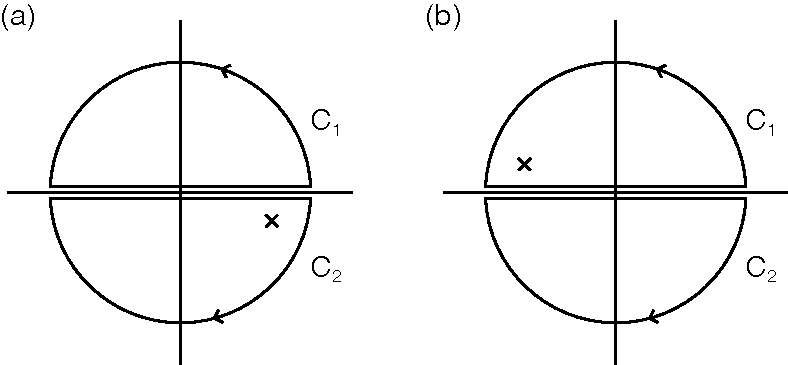
\includegraphics[width=0.6\textwidth]{resources/chap_green_0T/contour1.pdf}
		\caption{Contour integral for fermionic system. (a): the case $\tilde\epsilon_p>0$. (b): the case $\tilde\epsilon_p<0$}
		\label{fig:contour_fermion} 
	\end{figure}

	\subsection{Free Bosons}

	The Hamiltonian reads
	\begin{equation}
		H=\sum_{k\sigma}\omega_k a_k^\dagger a_k
	\end{equation}
	
	We have
	\begin{equation}
		|\Omega\rangle=a_0^{\dagger N}|0\rangle
	\end{equation}
	and
	\begin{equation}
		a_k(t)=e^{-i\omega_kt}a_k
	\end{equation}
	
	Let $\phi=a+a^\dagger$, we traditionally define
	\begin{equation}
		iG(x_j,t_j;x_i,t_i)=\langle \Omega|T[\phi(x_j,t_j)\phi(x_i,t_i)]|\Omega\rangle
	\end{equation}
	
	So
	\begin{eqnarray}
		&&iG(x_j,t_j;x_i,t_i)\\
		&=&\langle \Omega|a(x_j,t_j)a^\dagger(x_i,t_i)|\Omega\rangle\theta(t_f-t_i)+\langle \Omega|a^\dagger(x_j,t_j)a(x_i,t_i)|\Omega\rangle\theta(t_f-t_i)\nonumber\\
		&&+\langle \Omega|a(x_i,t_i)a^\dagger(x_j,t_j)|\Omega\rangle\theta(t_i-t_j)+\langle \Omega|a^\dagger(x_i,t_i)a(x_j,t_j)|\Omega\rangle\theta(t_i-t_j)\\
		&=&\int\frac{d^3p_j}{(2\pi)^3}\int\frac{d^3p_i}{(2\pi)^3}e^{ip_j\cdot x_j-ip_i\cdot x_i}\big[\langle \Omega|a(p_j,t_j)a^\dagger(p_i,t_i)|\Omega\rangle\theta(t_j-t_i)+\langle \Omega|a^\dagger(p_j,t_j)a(p_i,t_i)|\Omega\rangle\nonumber\\
		&&\theta(t_j-t_i)+\langle \Omega|a(p_i,t_i)a^\dagger(p_j,t_j)|\Omega\rangle\theta(t_i-t_j)+\langle \Omega|a^\dagger(p_i,t_i)a(p_j,t_j)|\Omega\rangle\theta(t_i-t_j)\big]\\
		&=&\int\frac{d^3p}{(2\pi)^3}e^{ip\cdot(x_j-x_i)}\big[\langle \Omega|a(p,t_j)a^\dagger(p,t_i)|\Omega\rangle\theta(t_j-t_i)+\langle \Omega|a^\dagger(p,t_j)a(p,t_i)|\Omega\rangle\nonumber\\
		&&\theta(t_j-t_i)+\langle \Omega|a(p,t_i)a^\dagger(p,t_j)|\Omega\rangle\theta(t_i-t_j)+\langle \Omega|a^\dagger(p,t_i)a(p,t_j)|\Omega\rangle\theta(t_i-t_j)\big]\\
		&=&\int\frac{d^3p}{(2\pi)^3}e^{ip\cdot(x_j-x_i)}\big[\langle \Omega|a(p)a^\dagger(p)|\Omega\rangle e^{-i\omega_p(t_j-t_i)}\theta(t_j-t_i)+\langle \Omega|a^\dagger(p)a(p)|\Omega\rangle e^{-i\omega_p(t_i-t_j)}\nonumber\\
		&&\theta(t_j-t_i)+\langle \Omega|a(p)a^\dagger(p)|\Omega\rangle e^{-i\omega_p(t_i-t_j)}\theta(t_i-t_j)+\langle \Omega|a^\dagger(p)a(p)|\Omega\rangle e^{-i\omega_p(t_j-t_i)}\theta(t_i-t_j)\big]\\
		&=&\int\frac{d^3p}{(2\pi)^3}e^{ip\cdot(x_j-x_i)}\big[e^{-i\omega_p(t_j-t_i)}\theta(t_j-t_i)+ e^{-i\omega_p(t_i-t_j)}\theta(t_i-t_j)\big]+N
	\end{eqnarray}
	
	Let's suppose $N=0$. Then
	\begin{equation}
		iG(x_j-x_i,t_j-t_i)=\int\frac{d^3p}{(2\pi)^3}e^{ip\cdot(x_j-x_i)}\big[e^{-i\omega_p(t_j-t_i)}\theta(t_j-t_i)+ e^{-i\omega_p(t_i-t_j)}\theta(t_i-t_j)\big]
	\end{equation}
	
	So
	\begin{eqnarray}
		iG(p,t_j-t_i)&=&\big[e^{-i\omega_p(t_j-t_i)}\theta(t_j-t_i)+ e^{-i\omega_p(t_i-t_j)}\theta(t_i-t_j)\big]\\
		&=&\frac 1{-2\pi i}\int d\omega e^{-i\omega(t_j-t_i)}\frac 1{\omega-\omega_p+i\delta}+\frac 1{2\pi i}\int d\omega e^{-i\omega(t_j-t_i)}\frac 1{\omega+\omega_p-i\delta}\\
		&=&\frac 1{-2\pi i}\int d\omega e^{-i\omega(t_j-t_i)}\Big(\frac 1{\omega-\omega_p+i\delta}-\frac 1{\omega+\omega_p-i\delta}\Big)\\
		&=&\frac 1{-2\pi i}\int d\omega e^{-i\omega(t_j-t_i)}\frac{2\omega_p}{\omega^2-(\omega_p-i\delta)^2}\\
		&=&\frac 1{-2\pi i}\int d\omega e^{-i\omega(t_j-t_i)}\frac{2\omega_p}{\omega^2-\omega_p^2+i\delta}
	\end{eqnarray}
	where $0<\delta\ll 1$.  We take the $C_1$ contour in Fig. \ref{fig:contour_boson} when $t_f-t_i<0$, abd $C_2$ contour when $t_f-t_i>0$
	
	\begin{figure}[htb]
		\centering  
		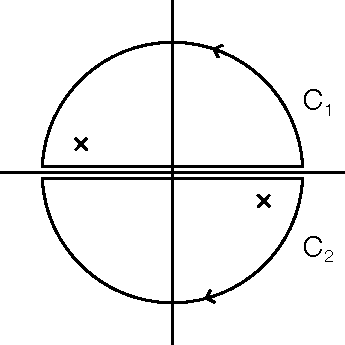
\includegraphics[width=0.3\textwidth]{resources/chap_green_0T/contour2.pdf}
		\caption{Contour integral for bosonic system}
		\label{fig:contour_boson} 
	\end{figure}
	
	So
	\begin{equation}
		G(p,\omega)=\frac{2\omega_p}{\omega^2-\omega_p^2+i\delta}
	\end{equation}
	\section{Different Green's Functions}
	\label{sec:0t_green}
	We use Lehmann spectral representation to study relation between different two-point Green's functions.
	
	\subsection{Feynman Propogator}
	\begin{eqnarray}
		iG(t)&=&\langle T[O_2(t)O_1(0)]\rangle\\
		&=&\langle O_2(t)O_1(0)\rangle\theta(t)+\eta\langle O_1(0)O_2(t)\rangle\theta(-t)\\
		&=&\sum_n\big[\langle \Omega|O_2(t)|n\rangle\langle n|O_1(0)|\Omega\rangle\theta(t)+\eta\langle \Omega|O_1(0)|n\rangle\langle n|O_2(t)|\Omega\rangle\theta(-t)\big]\\
		&=&\sum_n\big[e^{-it E_n}\theta(t)O_n+\eta e^{it E_n}\theta(-t)O'_n\big]\\
		&=&\int\frac{d\omega}{-2\pi i}e^{-it\omega}\sum_{n}\Big[\frac{O_n}{\omega-E_n+i\delta}-\frac{\eta O'_n}{\omega+E_n-i\delta}\Big]\\
		G(\omega)&=&\sum_n\Big[\frac{O_n}{\omega-E_n+i\delta}-\frac{\eta O'_n}{\omega+E_n-i\delta}\Big]\\
	\end{eqnarray}
	
	On the real axis,
	\begin{eqnarray}
		\Re G(\omega)&=&\sum_n\Big[P\frac{O_n}{\omega-E_n}-P\frac{\eta O'_n}{\omega+E_n}\Big]\\
		\Im G(\omega)&=&\sum_{n}\big[(-\pi)O_n\delta(\omega-E_n)-\eta\pi O'_n\delta(\omega+E_n)\big]\\
		&=&-\pi\sum_{n}\big[O_n\delta(\omega-E_n)+\eta O'_n\delta(\omega+E_n)\big]
	\end{eqnarray}
	\subsection{Retarded Green's Function}
	\begin{eqnarray}
		iG_R(t)&=&\langle [O_2(t),O_1(0)]_\eta\rangle\theta(t)\\
		&=&\big[\langle O_2(t)O_1(0)\rangle-\eta\langle O_1(0)O_2(t)\rangle\big]\theta(t)\\
		&=&\sum_{n}\big[\langle\Omega|O_2(t)|n\rangle\langle n|O_1(0)|\Omega\rangle-\eta\langle\Omega|O_1(0)|n\rangle\langle n|O_2(t)|\Omega\rangle\big]\theta(t)\\
		&=&\sum_n\big[e^{-it E_n}O_n-\eta e^{it E_n}O'_n\big]\theta(t)\\
		&=&\int\frac{d\omega}{-2\pi i}e^{-it\omega}\sum_{n}\Big[\frac{O_n}{\omega-E_n+i\delta}-\frac{\eta O'_n}{\omega+E_n+i\delta}\Big]\\
		G_R(\omega)&=&\sum_n\Big[\frac{O_n}{\omega-E_n+i\delta}-\frac{\eta O'_n}{\omega+E_n+i\delta}\Big]
	\end{eqnarray}
	
	On the real axis,
	\begin{eqnarray}
		\Re G_R(\omega)&=&\sum_n\Big[P\frac{O_n}{\omega-E_n}-P\frac{\eta O'_n}{\omega+E_n}\Big]\\
		\Im G_R(\omega)&=&\sum_{n}\big[(-\pi)O_n\delta(\omega-E_n)-\eta(-\pi)O'_n\delta(\omega+E_n)\big]\\
		&=&-\pi\sum_{n}\big[O_n\delta(\omega-E_n)-\eta O'_n\delta(\omega+E_n)\big]
	\end{eqnarray}
	
	For boson ($\eta=1$), then $n=0$ terms vanish. So the summation should be $\sum_{n\neq 0}$.
	\subsection{Advanced Green's Function}
	\begin{eqnarray}
		iG_A(t)&=&-\langle [O_2(t),O_1(0)]_\eta\rangle\theta(-t)\\
		&=&-\big[\langle O_2(t)O_1(0)\rangle-\eta\langle O_1(0)O_2(t)\rangle\big]\theta(-t)\\
		&=&-\sum_{n}\big[\langle\Omega|O_2(t)|n\rangle\langle n|O_1(0)|\Omega\rangle-\eta\langle\Omega|O_1(0)|n\rangle\langle n|O_2(t)|\Omega\rangle\big]\theta(-t)\\
		&=&-\sum_n\big[e^{-it E_n}O_n-\eta e^{it E_n}O'_n\big]\theta(-t)\\
		&=&\int\frac{d\omega}{-2\pi i}e^{-it\omega}\sum_{n}\Big[\frac{O_n}{\omega-E_n-i\delta}-\frac{\eta O'_n}{\omega+E_n-i\delta}\Big]\\
		G_A(\omega)&=&\sum_n\Big[\frac{O_n}{\omega-E_n-i\delta}-\frac{\eta O'_n}{\omega+E_n-i\delta}\Big]
	\end{eqnarray}
	
	On the real axis,
	\begin{eqnarray}
		\Re G_A(\omega)&=&\sum_n\Big[P\frac{O_n}{\omega-E_n}-P\frac{\eta O'_n}{\omega+E_n}\Big]\\
		\Im G_A(\omega)&=&\sum_{n}\big[\pi O_n\delta(\omega-E_n)-\eta\pi O'_n\delta(\omega+E_n)\big]\\
		&=&\pi\sum_{n}\big[O_n\delta(\omega-E_n)-\eta O'_n\delta(\omega+E_n)\big]
	\end{eqnarray}
	
	For boson ($\eta=1$), then $n=0$ terms vanish. So the summation should be $\sum_{n\neq 0}$.
	\subsection{Relation between Different Green's Functions}
	\begin{eqnarray}
		G_A(\omega)&=&G(\omega\rightarrow \omega-i\delta)\\
		G_R(\omega)&=&G(\omega\rightarrow \omega+i\delta)
	\end{eqnarray}
	
	On the real axis,
	\begin{eqnarray}
		\Re G(\omega)&=&\Re G_A(\omega)=\Re G_R(\omega)\\
		\Im G(\omega)&=&\Im G_R(\omega)H(\omega)=-\Im G_A(\omega)H(\omega)
	\end{eqnarray}
	where $H$ is the Heaviside step function.
	\subsection{Spectral Function}
	
	Let's define
	\begin{eqnarray}
		A(\omega)&=&2\Im G_A(\omega)\\
		&=&i(G_R(\omega)-G_A(\omega))\\
		&=&2\pi\sum_{n}\big[O_n\delta(\omega-E_n)-\eta O'_n\delta(\omega+E_n)\big]
	\end{eqnarray}
	
	We have
	\begin{eqnarray}
		\int \frac{d\omega}{2\pi} A(\omega)&=&O_n-\eta O'_n\\
		&=&\sum_n\big[\langle\Omega|O_2|n\rangle\langle n|O_1|\Omega\rangle-\eta\langle\Omega|O_1|n\rangle\langle n|O_2|\Omega\rangle\big]\\
		&=&\langle [O_2,O_1]_\eta\rangle
	\end{eqnarray}
	
	So $\int \frac{d\omega}{2\pi} A(\omega)=1$ if $O_2$ and $O_1$ is a canonical pair.
	
	We can reconstruct the Green's function just from $A(\omega)$ (on real axis) by the contour integral method.
	
	Since $A(\omega)=i(G_R(\omega)-G_A(\omega))$
	\begin{eqnarray}
		\int \frac{d\omega}{2\pi}(n_\eta^-\theta(\tau)+n_\eta^+\theta(-\tau)) A(\omega)e^{-\omega \tau}&=&i\int_C \frac{d\omega}{2\pi}(n_\eta^-\theta(\tau)+n_\eta^+\theta(-\tau)) \mathcal G(\omega)e^{-\omega \tau}\\
		&=&\frac 1\beta\sum_n\mathcal G(i\omega_n)e^{-i\omega_n \tau}\\
		&=&\mathcal G(\tau)
	\end{eqnarray}
	where $C$ is the clockwise contour around the real axis.
	
	\subsection{Correlation Function}
	
	\begin{eqnarray}
		S(t)&=&\langle O_2(t) O_1(0)\rangle\\
		&=&\sum_n\langle \Omega|O_2(t)|n\rangle\langle n|O_1(0)|\Omega\rangle\\
		&=&\sum_ne^{-it E_n}O_n\\
		&=&\int\frac{d\omega}{-2\pi i}e^{-it\omega}\sum_{n}\Big[\frac{O_n}{\omega-E_n+i\delta}-\frac{O_n}{\omega-E_n-i\delta}\Big]\\
		&=&\int d\omega e^{-it\omega}\sum_{n}O_n\delta(\omega-E_n)\\
		S(\omega)&=&2\pi\sum_{n}O_n\delta(\omega-E_n)\\
	\end{eqnarray}
	
	We have
	\begin{equation}
		S(\omega)=-2\theta(\omega)\Im G_R(\omega)
	\end{equation}
			
	\section{Green's Function of Interacting System, the Gell-Mann-Low Theorem}
	
	Consider a quantum field be defined by Hamiltonian $H=H_0+H_{int}$. As long as we only consider event that happened at finite past/future, we may modify it as $H(t)=H_0+e^{-\epsilon t}H_{int}$ and let the small variable $\epsilon\rightarrow 0$ after the calculation.

	Since $\epsilon\ll 1$, $H(t)$ satisfy adiabatic evolvement theorem. So we have
	\begin{equation}
		U_H(-\infty \rightarrow 0)|0\rangle=e^{i\alpha}|\Omega\rangle
	\end{equation}
	where $|0\rangle$ is the (unique) vacuum state of $H_0$ and $|\Omega\rangle$ is the (unique) vacuum state of $H(0)=H_0+H_{int}$.
	
	Then
	\begin{equation}
		S_H(-\infty \rightarrow 0)|0\rangle=U_H(-\infty \rightarrow 0)U_{H_0}(0 \rightarrow -\infty)|0\rangle=e^{i\theta}|\Omega\rangle
	\end{equation}
	
	Then we can simplify the Green's function as
	\begin{eqnarray}
		iG(x_1,\dots,x_n)&=&\langle T[O_{1,H}(x_1)\cdots O_{n,H}(x_n)]\rangle\\
		&=&\langle\Omega| ph(p) O_{p_1,H}(x_{p_1})\cdots O_{p_n,H}(x_{p_n})|\Omega\rangle\\
		&=&\langle 0|ph(p)S_H(0\rightarrow -\infty) S_H(t_{p_1}\rightarrow 0)O_{p_1,I}(x_{p_1})S_H(0\rightarrow t_{p_1})\cdots \nonumber\\
		&&S_H(t_{p_n}\rightarrow 0)O_{p_n,I}(x_{p_n})S_H(0\rightarrow t_{p_n})S_H(-\infty \rightarrow 0)|0\rangle\\
		&=&\langle 0|S_H(\infty\rightarrow -\infty)ph(p)S_H(t_{p_1}\rightarrow \infty)O_{p_1,I}(x_{p_1})S_H(t_{p_2}\rightarrow t_{p_1})\cdots \nonumber\\
		&&S_H(t_{p_n}\rightarrow t_{p_{n-1}})O_{p_n,I}(x_{p_n})S_H(-\infty \rightarrow t_{p_n})|0\rangle\\
		&\stackrel{\rm formally}{=}&\langle 0|S_H(\infty\rightarrow -\infty) T[S_H(-\infty\rightarrow \infty)O_{1,I}(x_1)\cdots O_{n,I}(x_n)]|0\rangle
	\end{eqnarray}
	where $ph(p_i)$ is the phase factor ($\pm 1$) generated by the permutation $O_1 \dots O_n\rightarrow O_{p_1},\dots,O_{p_n}$. $x$ here are 4-vectors.
	
	Since $|0\rangle$ is unique, $\langle 0|S_H(\infty\rightarrow -\infty)=\langle 0|e^{i\phi}$. So
	\begin{equation}
		\langle 0|S_H(\infty\rightarrow -\infty)=\frac{\langle 0|}{\langle 0|S_H(-\infty\rightarrow \infty)|0\rangle}
	\end{equation}
	
	So
	\begin{equation}
		iG(x_1,\dots,x_n)=\frac{\langle 0|T[S_H(-\infty\rightarrow \infty)O_{1,I}(x_1)\cdots O_{n,I}(x_n)]|0\rangle}{\langle 0|S_H(-\infty\rightarrow \infty)|0\rangle}
	\end{equation}
	
	Actually it's easy to see that 
	\begin{equation}
		\langle 0|S_H(-\infty\rightarrow \infty)|0\rangle=\lim_{T\rightarrow \infty}\langle 0|S_H(-T\rightarrow T)|0\rangle=\lim_{T\rightarrow \infty}e^{iE_02T}\langle 0|U_H(-T\rightarrow T)|0\rangle=\lim_{T\rightarrow \infty}e^{-i\Delta E2T+i\gamma}
	\end{equation}
	where $\Delta E$ is the interaction energy and $\gamma$ is the Berry's phase.
	
	So we have
	\begin{equation}
		\Delta E=\lim_{T\rightarrow \infty}\frac i{2T}\ln\langle 0|S_H(-T\rightarrow T)|0\rangle
	\end{equation}
	
	\section{Perturbative Expansion and Wick's Theorem}
	We first learn how to treat $S_H(-\infty\rightarrow \infty)$ with perturbative expansion.
	\subsection{Perturbative Expansion}
	
	From Eqn. \ref{eqn:s_evolve}, we have the recursive formula
	\begin{equation}
		S_H(t_1\rightarrow t_2)=I+(-i)\int_{t_1}^{t_2}d\tau_1H_{int,I}(\tau_1)S_H(t_1\rightarrow \tau_1)
	\end{equation} 
	
	Then, if $H_{int}$ is relatively small compared to $H_0$, we have
	\begin{eqnarray}
		S_H(t_1\rightarrow t_2)&=&I+(-i)\int_{t_1}^{t_2}d\tau_1H_{int,I}(\tau_1)\nonumber \\
		&&+(-i)^2\int_{t_1}^{t_2}d\tau_1\int_{t_1}^{\tau_1}d\tau_2H_{int,I}(\tau_1)H_{int,I}(\tau_2)+\dots
	\end{eqnarray}
	
	Since $H_{int}$ is a bosonic operator, we have
	\begin{eqnarray}
		&\int_{t_1}^{t_2}d\tau_1\int_{t_1}^{\tau_1}d\tau_2\cdots\int_{t_1}^{\tau_{n-1}}d\tau_nH_{int,I}(\tau_1)H_{int,I}(\tau_2)\cdots H_{int,I}(\tau_n)\nonumber \\
		=&\frac 1{n!}\int_{t_1}^{t_2}d\tau_1\int_{t_1}^{t_2}d\tau_2\cdots\int_{t_1}^{t_2}d\tau_n T[H_{int,I}(\tau_1)H_{int,I}(\tau_2)\cdots H_{int,I}(\tau_n)]
	\end{eqnarray}
	
	So formally
	\begin{eqnarray}
		S_H(t_1\rightarrow t_2)&=&I+(-i)\int_{t_1}^{t_2}d\tau_1H_{int,I}(\tau_1)+\frac 1{2!}T\Big[(-i)\int_{t_1}^{t_2}d\tau_1H_{int,I}(\tau_1)\Big]^2+\dots\\
		&=&T\Big[e^{-i\int_{t_1}^{t_2}d\tau H_{int,I}(\tau)}\Big]
	\end{eqnarray}
	
	So the Green's function becomes
	\begin{eqnarray}
		iG(x_1,\dots,x_n)&=&\frac{\langle 0|T\big[e^{-i\int_{-\infty}^\infty d\tau H_{int,I}(\tau)}O_{1,I}(x_1)\cdots O_{n,I}(x_n)\big]|0\rangle}{\langle 0|T\big[e^{-i\int_{-\infty}^\infty d\tau H_{int,I}(\tau)}\big]|0\rangle}\\
		&=&\frac{\langle 0|T\big[\sum_{n=0}^\infty \frac{(-i)^n}{n!}\prod_{j=1}^n\int_{-\infty}^\infty d\tau_j H_{int,I}(\tau_j)O_{1,I}(x_1)\cdots O_{n,I}(x_n)\big]|0\rangle}{\langle 0|T\big[\sum_{n=0}^\infty\frac{(-i)^n}{n!}\prod_{j=1}^n\int_{-\infty}^\infty d\tau_j H_{int,I}(\tau_j)\big]|0\rangle}
	\end{eqnarray}
	
	Note that $O_I$ coincides with $O_H$ in the Heisenberg picture of $H_0$. So we can pretend that we are still doing the free model, and $H_{int}$ is nothing but a special operator $O$. Using the old technique, the Green's function can be calculated exactly to any order.
	
	However, instead of direct calculation, we can make our life easier by the following Wick's theorem.
	
	\subsection{Wick's Theorem}
	In this section we omit the I subscript of operators. $O$ are always assumed to be $O_I$.
	
	If we can break $O(t)$ into $O^+(t)+O^-(t)$ which satisfies:
	\begin{eqnarray}
		&&O^-(t)|0\rangle=0\\
		&&\langle 0|O^+(t)=0\\
		&&[O^+_1(t_1),O^+_2(t_2)]_\eta=[O^-_1(t_1),O^-_2(t_2)]_\eta=0 \label{eqn:wick_commute}
	\end{eqnarray}
	The time ordered product of n operators is defined as
	\begin{equation}
		T[O_1(t_1)\cdots O_n(t_n)]=ph(q)O_{q_1}(t_{q_1})\cdots O_{q_n}(t_{q_n})
	\end{equation}
	where $t_{q_1}>\cdots>t_{q_n}$
	
	We define the normal ordered product of n operators is defined as
	\begin{eqnarray}
		:O_1(t_1)\cdots O_n(t_n):&=&:\prod_{i=1}^n\sum_{\sigma=-}^+O_i^\sigma(t_i):\\
		&=&\sum_{\{\sigma_i\}}:\prod_{i=1}^nO_i^{\sigma_i}(t_i):\\
		&=&\sum_{\{\sigma_i\}}ph(p_{\{\sigma\}})\prod_{i=1}^nO_{p_{\{\sigma\}}(i)}^{\sigma_{p_{\{\sigma\}}(i)}}(t_{p_{\{\sigma\}}(i)})\\
	\end{eqnarray}
	where $p_{\{\sigma\}}$ is a permutation of 1 \dots n that depends on $\{\sigma\}$ such that $\sigma_{p_{\{\sigma\}}(1)}=\cdots=\sigma_{p_{\{\sigma\}}(m)}=+$ and $\sigma_{p_{\{\sigma\}}(m+1)}= \cdots=\sigma_{p_{\{\sigma\}}(n)}=-$. This is well-defined because of \ref{eqn:wick_commute}.
	
	Then we define Wick contraction as
	\begin{eqnarray}
		\contraction{}{O}{{}_1(t_1)}{O}
		O_1(t_1)O_2(t_2)&=&\left\{\begin{array}{ll}
			[O_1^-(t_1),O_2^+(t_2)]_\eta&(t_1>t_2)\\
			(-1)^\eta[O_2^-(t_2),O_1^+(t_1)]_\eta&(t_1<t_2)\\
		\end{array} \right. \\
		\contraction{}{O}{{}_1(t_1)\prod_i O_i(t_i)}{O}
		\contraction{O_1(t_1)\prod_i O_i(t_i)O_2(t_2)\quad=(-1)^{\sum_{i}\eta_i\eta_1} \prod_i O_i(t_i) }{O}{{}_1(t_1)}{O}
		O_1(t_1)\prod_i O_i(t_i)O_2(t_2)&=&(-1)^{\sum_{i}\eta_i\eta_1} \prod_i O_i(t_i) O_1(t_1)O_2(t_2) \label{eqn:wick_sandwich}
	\end{eqnarray}
	
	The definition is readily generalized to multiple Wick contractions in a product: just do Wick contractions in sequence using \ref{eqn:wick_sandwich}.
	
	It's easy to see that 
	\begin{equation}
		\contraction{}{O}{{}_1(t_1)}{O}
		\contraction{O_1(t_1)O_2(t_2)=(-1)^\eta }{O}{{}_2(t_2)}{O}
		O_1(t_1)O_2(t_2)=(-1)^\eta O_2(t_2)O_1(t_1)
	\end{equation}
	
	The Wick's theorem states that
	\begin{theorem}[Wick]
		\begin{equation}
			T[O_1(t_1)\cdots O_n(t_n)]=:{\rm all\ possible\ contractions\ of\ }O_1(t_1)\cdots O_n(t_n):
		\end{equation}
		where Wick contracted operators are not taken into consideration in normal ordering.
	\end{theorem}
	\begin{proof}
		We prove the theorem by induction on the number of operators. 
		
		First we observe
		\begin{eqnarray}
			T[O_1(t_1)]&=&O_1(t_1)\\
			\contraction{T[O_1(t_1)O_2(t_2)]=\quad}{O}{{}_1(t_1)}{O}
			T[O_1(t_1)O_2(t_2)]&=&O_1(t_1)O_2(t_2)+:O_1(t_1)O_2(t_2):\\
		\end{eqnarray}
		
		So the theorem is valid for product of 1 and 2 operators. Assume the theorem is valid for product of n-1 operators, we need to prove
		\begin{equation}
			T[O_1(t_1)\cdots O_n(t_n)]=:{\rm all\ possible\ contractions\ of\ }O_1(t_1)\cdots O_n(t_n):
		\end{equation}
		
		Assume $t_m$ is the largest among $t_1\dots t_n$
		\begin{eqnarray}
			T[O_1(t_1)\cdots O_n(t_n)]
			&=&(-1)^{\sum_{i<m}\eta_i\eta_m} O_m(t_m)T\Big[\prod_{j\neq m}O_j(t_j)\Big]\\
			&=&:{\rm all\ possible\ contractions\ of\ }\prod_{j}O_j(t_j){\rm\ such \ that\ }O_m(t_m){\rm\ is \ uncontracted}\nonumber \\
			&&{\rm and\ has\ a\ plus\ sign}:+(-1)^{\sum_{i<m}\eta_i\eta_m} O^-_m(t_m):{\rm all\ possible\ contractions}\nonumber \\
			&&{\rm of}\prod_{j\neq m}O_j(t_j):
		\end{eqnarray}
		
		It's not hard to see that
		\begin{eqnarray}
			&&(-1)^{\sum_{i<m}\eta_i\eta_m} O^-_m(t_m):{\rm all\ possible\ contractions\ of\ }\prod_{j\neq m}O_j(t_j):\\
			&=&:{\rm all\ possible\ contractions\ of\ }\prod_{j}O_j(t_j){\rm\ such\ that\ }O_m(t_m){\rm\ is \ uncontracted\ and\ has\ a}\nonumber \\
			&&{\rm minux\ sign}:+:{\rm all\ possible\ contractions\ of\ }\prod_{j}O_j(t_j){\rm\ with\ }O_m(t_m){\rm \ contracted}:
		\end{eqnarray}
		
		So 
		\begin{equation}
			T[O_1(t_1)\cdots O_n(t_n)]=:{\rm all\ possible\ contractions\ of\ }O_1(t_1)\cdots O_n(t_n):
		\end{equation}
	\end{proof}
	
	For example
	\begin{eqnarray}
		\contraction{T[O_1(t_1)O_2(t_2)O_3(t_3)]=\quad\ :}{O}{{}_1(t_1)}{O}
		\contraction{T[O_1(t_1)O_2(t_2)O_3(t_3)]=\quad\ :O_1(t_1)O_2(t_2)O_3(t_3):+:}{O}{{}_1(t_1)O_2(t_2)}{O}
	T[O_1(t_1)O_2(t_2)O_3(t_3)]&=&:O_1(t_1)O_2(t_2)O_3(t_3):+:O_1(t_1)O_2(t_2)O_3(t_3):+\nonumber\\
		\contraction{\qquad\,  :O_1(t_1)}{O}{{}_2(t_2)}{O}
		&&:O_1(t_1)O_2(t_2)O_3(t_3):+:O_1(t_1)O_2(t_2)O_3(t_3):\\
		\contraction{T[O_1(t_1)O_2(t_2)O_3(t_3)O_4(t_4)]=\quad\ :}{O}{{}_1(t_1)}{O}
		\contraction{T[O_1(t_1)O_2(t_2)O_3(t_3)O_4(t_4)]=\quad\ :O_1(t_1)O_2(t_2)}{O}{{}_3(t_3)}{O}
		\contraction{T[O_1(t_1)O_2(t_2)O_3(t_3)O_4(t_4)]=\quad\ :O_1(t_1)O_2(t_2)O_3(t_3)O_4(t_4):+:}{O}{{}_1(t_1)O_2(t_2)}{O}
		\contraction[2ex]{T[O_1(t_1)O_2(t_2)O_3(t_3)O_4(t_4)]=\quad\ :O_1(t_1)O_2(t_2)O_3(t_3)O_4(t_4):+:O_1(t_1)}{O}{{}_2(t_2)O_3(t_3)}{O}
	T[O_1(t_1)O_2(t_2)O_3(t_3)O_4(t_4)]&=&:O_1(t_1)O_2(t_2)O_3(t_3)O_4(t_4):+:O_1(t_1)O_2(t_2)O_3(t_3)O_4(t_4):+\nonumber\\
		\contraction[2ex]{\qquad\, :}{O}{{}_1(t_1)O_2(t_2)O_3(t_3)}{O}
		\contraction{\qquad\, :O_1(t_1)}{O}{{}_2(t_2)}{O}
		\contraction{\qquad\, :O_1(t_1)O_2(t_2)O_3(t_3)O_4(t_4):+:}{O}{{}_1(t_1)}{O}
		&&:O_1(t_1)O_2(t_2)O_3(t_3)O_4(t_4):+:O_1(t_1)O_2(t_2)O_3(t_3)O_4(t_4):+\nonumber\\
		\contraction{\qquad\, :}{O}{{}_1(t_1)O_2(t_2)}{O}
		\contraction{\qquad\, :O_1(t_1)O_2(t_2)O_3(t_3)O_4(t_4):+:}{O}{{}_1(t_1)O_2(t_2)O_3(t_3)}{O}
		&&:O_1(t_1)O_2(t_2)O_3(t_3)O_4(t_4):+:O_1(t_1)O_2(t_2)O_3(t_3)O_4(t_4):+\nonumber\\
		\contraction{\qquad\, :O_1(t_1)}{O}{{}_2(t_2)}{O}
		\contraction{\qquad\, :O_1(t_1)O_2(t_2)O_3(t_3)O_4(t_4):+:O_1(t_1)}{O}{{}_2(t_2)O_3(t_3)}{O}
		&&:O_1(t_1)O_2(t_2)O_3(t_3)O_4(t_4):+:O_1(t_1)O_2(t_2)O_3(t_3)O_4(t_4):+\nonumber\\
		\contraction{\qquad\, :O_1(t_1)O_2(t_2)}{O}{{}_3(t_3)}{O}
		&&:O_1(t_1)O_2(t_2)O_3(t_3)O_4(t_4):+:O_1(t_1)O_2(t_2)O_3(t_3)O_4(t_4):
	\end{eqnarray}
	
	Obviously we have 
	\begin{eqnarray}
		iG^0_{12}(t_1,t_2)&=&\langle0|T[O_1(t_1)O_2(t_2)]|0\rangle\\
		\contraction{\qquad\ \, \langle0|}{O}{{}_1(t_1)}{O}
		&=&\langle0|O_1(t_1)O_2(t_2)|0\rangle
	\end{eqnarray}
	where $G^0$ means Green's function of free system
	
	We call operators simple if they satisfy
	\begin{equation}
		\contraction{}{O}{{}_1(t_1)}{O}
		\contraction{O_1(t_1)O_2(t_2)|0\rangle=|0\rangle\langle0|}{O}{{}_1(t_1)}{O}
		O_1(t_1)O_2(t_2)|0\rangle=|0\rangle\langle0|O_1(t_1)O_2(t_2)|0\rangle
	\end{equation}
	
	Then
	\begin{eqnarray}
		\langle 0|T[O_1(t_1)\cdots O_n(t_n)]|0\rangle &=&\langle 0|:{\rm all\ full\ contractions\ of\ }O_1(t_1)\cdots O_n(t_n):|0\rangle\\
		\contraction{\qquad\;  \sum_{\{p\}}ph(p)\prod_i\langle0|}{O}{{}_{p_{i,1}}(t_{p_{i,1}})}{O}
		&=&\sum_{\{p\}}ph(p)\prod_i \langle0|O_{p_{i,1}}(t_{p_{i,1}})O_{p_{i,2}}(t_{p_{i,2}})|0\rangle\\
		&=&\sum_{\{p\}}ph(p)\prod_i iG_{p_{i,1}p_{i,2}}(t_{p_{i,1}},t_{p_{i,2}})
	\end{eqnarray}
	where full contractions means every operator is Wick contracted, $\{p_i\}$ is pairs that 1 \dots n can be divided into and $ph(p)$ is some phase factor decided by $\{p_i\}$.
	
	For example, if all operators are fermionic operators
	\begin{eqnarray}
		iG^0_{1234}(t_1,t_2,t_3,t_4)&=&\langle 0|T[O_1(t_1)O_2(t_2)O_3(t_3)O_4(t_4)]|0\rangle\\
		&=&iG^0_{12}(t_1,t_2)iG^0_{34}(t_3,t_4)-iG^0_{13}(t_1,t_3)iG^0_{24}(t_2,t_4)\nonumber\\
		&& +iG^0_{14}(t_1,t_4)iG^0_{23}(t_2,t_3)
	\end{eqnarray}
	
	\chapter{Functional Field Integral}
	
	In this chapter, the space is always discretized into $3N$ points
	
	\section{Path Integral of the Scalar Field}
	
	Let $\hat\phi(x)$ $(x\in\mathbb R^3)$ be a bosonic field operator. That is, one with eigen-states $|\phi(x)\rangle$, such that 
	\begin{equation}
		\hat\phi(x)|\phi(x)\rangle=\phi(x)|\phi(x)\rangle
	\end{equation}
	and 
	\begin{equation}
		1=\int d\phi(x) |\phi(x)\rangle\langle \phi(x)|
	\end{equation}
	where the $|\phi(x)\rangle\langle \phi(x)|$ integrated over all $\phi(x)$.
	
	Let the Hamiltonian be 
	\begin{equation}
		H=\int d^3x\frac 12 \pi^2+V(\phi)
	\end{equation}
	
	Then
	\begin{eqnarray}
		\langle \phi_j|U(t_i\rightarrow t_i+\Delta t)|\phi_i\rangle&=&\langle \phi_j|e^{-iH\Delta t}|\phi_i\rangle\\
		&=&\int\frac {d\pi}{(2\pi)^{3N}}\langle \phi_j|\pi\rangle\langle \pi|e^{-iH\Delta t}|\phi_i\rangle\\
		&=&\int\frac {d\pi}{(2\pi)^{3N}}e^{i\int d^3x\pi \phi_j}e^{-i(\frac {\pi^2}{2}+V(\pi_i))\Delta t}e^{-i\int d^3x \pi \phi_i}\\
		&=&\int\frac {d\pi}{(2\pi)^{3N}}e^{i(\pi\frac {\Delta \phi}{\Delta t}-\frac {\pi^2}{2m}-V(\phi_i))\Delta t}\\
		&=&\bigg(\sqrt{\frac1{2\pi i\Delta t}}\bigg)^{3N}e^{i(\frac 12(\frac{\Delta \phi}{\Delta t})^2-V(\phi_i))\Delta t}\\
		&=&\bigg(\sqrt{\frac1{2\pi i\Delta t}}\bigg)^{3N}e^{iL(\phi_i,\partial_0 \phi_i)\Delta t}
	\end{eqnarray}
	
	So
	
	\begin{eqnarray}
		\langle \phi_j|U(t_i\rightarrow t_j)|\phi_i\rangle&=& \langle \phi_j|U(t_N\rightarrow t_j)|\phi_N\rangle\cdots \langle \phi_2|U(t_1 \rightarrow t_2)|x_1\rangle \langle \phi_1|U(t_i \rightarrow t_1)|\phi_i\rangle\\
		&=&\int\prod d\phi_i\bigg(\sqrt{\frac{m}{2\pi i\Delta t}}\bigg)^{V(N+1)}e^{\sum_n iL( \phi_n,\partial_0  \phi_n,t_n)\Delta t}\\
		&=&\bigg(\sqrt{\frac{m}{2\pi i\Delta t}}\bigg)^V\int \mathcal D\bigg(\bigg(\sqrt{\frac{m}{2\pi i\Delta t}}\bigg)^V\phi\bigg)e^{i\int_{t_i}^{t_j}dtL(\phi,\partial_0 \phi,t)}
	\end{eqnarray}
	
	Besides, let $O_i(\phi)$ be a function of $\phi$, then
	\begin{equation}
		\langle \phi_j|U(t_j,0)T[\prod_nO_H(t_n)]U(0,t_i)|\phi_i\rangle=C\int \mathcal D \phi\prod_n O(\phi(t_n))e^{i\int_{t_i}^{t_j}dtL(\phi,\partial_0 \phi,t)}
	\end{equation}
	where $t_i<t_n<t_j$
	
	\section{Path Integral of the Spinor Field}
	Let $\hat\psi(x)$ $(x\in\mathbb R^3)$ be a fermionic field operator. Let
	\begin{eqnarray}
		|\eta\rangle&=&e^{\int dx-\eta(x)\hat\psi^\dagger(x)}|0\rangle\\
		\langle\bar\eta|&=&\langle0|e^{\int dx\bar\eta(x)\hat\psi(x)}
	\end{eqnarray}
	be the corresponding coherent states.
	
	Then
	\begin{eqnarray}
		\langle\bar\eta_j|U(t_i\rightarrow t_i+\Delta t)|\eta_i\rangle&=&\langle\bar\eta_j|e^{-iH\Delta t}|\eta_i\rangle\\
		&\simeq&\langle\bar\eta_j|(1-iH\Delta t)|\eta_i\rangle\\
		&=&e^{\int dx\bar\eta_j\eta_i-iH(\bar\eta_j,\eta_i)\Delta t}
	\end{eqnarray}
	
	So
	
	\begin{eqnarray}
		\langle \bar\eta|U(t_i\rightarrow t_j)|\eta\rangle&=&\int\prod_i(d\bar\eta_id\eta_i) \langle \bar\eta|U(t_N\rightarrow t_j)|\eta_N\rangle e^{-\int dx\bar\eta_N(x)\eta_N(x)}\cdots \langle \bar\eta_2|U(t_1 \rightarrow t_2)|\eta_1\rangle\nonumber\\
		 &&e^{-\int dx\bar\eta_1(x)\eta_1(x)}\langle \bar\eta_1|U(t_i \rightarrow t_1)|\eta\rangle\\
		&\simeq&\int\prod_i(d\bar\eta_id\eta_i)\prod_ie^{-\int dx\bar\eta_i\Delta\eta_i-iH(\bar\eta_i,\eta_i)\Delta t}\\
		&\simeq&\int \mathcal D(\bar\eta,\eta)e^{i\int_{t_i}^{t_j}dt(i\int dx\bar\eta\dot\eta-H(\bar\eta,\eta))}\\
		&=&\int \mathcal D(\bar\eta,\eta)e^{i\int_{t_i}^{t_j}dtL}
	\end{eqnarray}
	
	Besides, let $O_i(\psi,\psi^\dagger)$ be a function of $\psi$ in normal order, then
	\begin{equation}
		\langle \bar\eta|U(t_j,0)T[\prod_nO_H(t_n)]U(0,t_i)|\eta\rangle=C\int \mathcal D \phi\prod_n O(\bar\eta(t_n),\eta(t_n))e^{i\int_{t_i}^{t_j}dtL}
	\end{equation}
	where $t_i<t_n<t_j$
	
	\section{Path Integral Representation of the Green's Function}
	
	
	We have
	\begin{equation}
		\langle j|U(t_j,0)T[\prod_nO_H(t_n)]U(0,t_i)|i\rangle=C\int \mathcal D \phi\prod_n O(\phi(t_n))e^{i\int_{t_i}^{t_j}dtL}
	\end{equation}
	
	We can insert $1=|n\rangle\langle n|$ in energy representation
	\begin{equation}
		\langle j|U(t_j,0)T[\prod_nO_H(t_n)]U(0,t_i)|i\rangle=\langle j|U(t_j,0)|m\rangle\langle m|T[\prod_nO_H(t_n)]|n\rangle\langle n|U(0,t_i)|i\rangle
	\end{equation}
	
	We may complexify $t$, and integrate $t$ along the path $-T(1-i\epsilon)$ to $T(1-i\epsilon)$. That is
	\begin{equation}
		\langle j|U(T(1-i\epsilon),0)|m\rangle\langle m|T[\prod_nO_H(t_n)]|n\rangle\langle n|U(0,-T(1-i\epsilon))|i\rangle=C\int \mathcal D \phi\prod_n O(\phi(t_n))e^{i\int_{-T(1-i\epsilon)}^{T(1-i\epsilon)}dtL} \label{eqn:green_path}
	\end{equation}

	It's easy to see
	\begin{eqnarray}
		\lim_{T\rightarrow \infty}\langle j|U(T(1-i\epsilon),0)|m\rangle &=& \lim_{T\rightarrow \infty}\langle j|U(T(1-i\epsilon),0)|\Omega\rangle\delta_{m0}\\
		\lim_{T\rightarrow \infty}\langle n|U(0,-T(1-i\epsilon))|i\rangle &=& \lim_{T\rightarrow \infty}\langle \Omega|U(0,-T(1-i\epsilon))|i\rangle\delta_{n0}
	\end{eqnarray}
	
	So the LHS of (\ref{eqn:green_path}) becomes
	\begin{eqnarray}
		&&\lim_{T\rightarrow \infty}\langle j|U(T(1-i\epsilon),0)|m\rangle\langle m|T[\prod_nO_H(t_n)]|n\rangle\langle n|U(0,-T(1-i\epsilon))|i\rangle\\
		&=&\lim_{T\rightarrow \infty}\langle j|U(T(1-i\epsilon),0)|\Omega\rangle\langle \Omega|T[\prod_nO_H(t_n)]|\Omega\rangle\langle \Omega|U(0,-T(1-i\epsilon))|i\rangle\\
		&=&\langle \Omega|T[\prod_nO_H(t_n)]|\Omega\rangle\lim_{T\rightarrow \infty}\langle j|U(T(1-i\epsilon),0)|\Omega\rangle\langle \Omega|U(0,-T(1-i\epsilon))|i\rangle\\
		&=&\langle \Omega|T[\prod_nO_H(t_n)]|\Omega\rangle\lim_{T\rightarrow \infty}\langle j|U(T(1-i\epsilon),0)|n\rangle\langle n|U(0,-T(1-i\epsilon))|i\rangle\\
		&=&\langle \Omega|T[\prod_nO_H(t_n)]|\Omega\rangle\lim_{T\rightarrow \infty}\langle j|U(T(1-i\epsilon),-T(1-i\epsilon))|i\rangle
	\end{eqnarray}
	when taking the limit $T\rightarrow \infty$.
	
	So
	\begin{equation}
		\langle \Omega|T[\prod_nO_H(t_n)]|\Omega\rangle\lim_{T\rightarrow \infty}\langle j|U(T(1-i\epsilon),-T(1-i\epsilon))|i\rangle=C\int \mathcal D \phi\prod_n O(\phi(t_n))e^{i\int_{-\infty(1-i\epsilon)}^{\infty(1-i\epsilon)}dtL}
	\end{equation}
	
	Without any $O$, we have
	\begin{equation}
		\lim_{T\rightarrow \infty}\langle j|U(T(1-i\epsilon),-T(1-i\epsilon))|i\rangle=C\int \mathcal D \phi e^{i\int_{-\infty(1-i\epsilon)}^{\infty(1-i\epsilon)}dtL}
	\end{equation}
	
	So the Green's function becomes
	\begin{eqnarray}
		\langle \Omega|T[\prod_nO_H(t_n)]|\Omega\rangle&=&\frac{\int \mathcal D \phi\prod_n O(\phi(t_n))e^{i\int_{-\infty(1-i\epsilon)}^{\infty(1-i\epsilon)}dtL}}{\int \mathcal D \phi e^{i\int_{-\infty(1-i\epsilon)}^{\infty(1-i\epsilon)}dtL}}\\
		&=&\frac 1Z\int \mathcal D \phi\prod_n O(\phi(t_n))e^{i\int_{-\infty(1-i\epsilon)}^{\infty(1-i\epsilon)}dtL}
	\end{eqnarray}
	where $Z=\int \mathcal D \phi e^{i\int_{-\infty(1-i\epsilon)}^{\infty(1-i\epsilon)}dtL}$
	
	
	\section{Generating Functional Method}
	
	The generating functional of the Green's function is the path integral with source term $J(x,t)$. The Green's function can be expressed by the functional derivative of the generating functional. 
	
	\subsection{The Free Bosonic System}
	
	For the free bosonic system, we study
	\begin{equation}
		\int \mathcal D \phi\prod_n \phi(x_n,t_n)e^{i\int_{-\infty(1-i\epsilon)}^{\infty(1-i\epsilon)}dtL}
	\end{equation}
	
	We define the generating functional as
	\begin{equation}
		Z[J]=\int \mathcal D \phi e^{i\int_{-\infty(1-i\epsilon)}^{\infty(1-i\epsilon)}dt[L+\int d^3x\phi(x,t)J(x,t)]}
	\end{equation}
	
	In a free system, $\int dt L=\frac 12\int d^4xd^4x'\phi(x)A(x,x')\phi(x')$ is a bilinear form of $\phi$. Then
	\begin{equation}
		Z[J]=Z\int \mathcal D \phi e^{i\frac 12\int d^4xd^4x'iJ(x)A^{-1}(x,x')iJ(x')}
	\end{equation}
	
	The average of $\prod_n \phi(x_n,t_n)$ can be evaluate by the functional derivative of $Z[J]$ by the source term.
	\begin{eqnarray}
		\langle \Omega|T[\prod_n\phi(x_n,t_n)]|\Omega\rangle&=&\frac 1Z\int \mathcal D \phi\prod_n \phi(x_n,t_n)e^{i\int_{-\infty(1-i\epsilon)}^{\infty(1-i\epsilon)}dtL}\\
		&=&\frac 1Z\int \mathcal D \phi\prod_n \frac\delta{i\delta J(x_n,t_n)}e^{i\int_{-\infty(1-i\epsilon)}^{\infty(1-i\epsilon)}dt\int d^3x[\mathcal L+\phi(x,t)J(x,t)]}\Big|_{J=0}\\
		&=&\frac 1Z\prod_n \frac\delta{i\delta J(x_n,t_n)}Z[J]\Big|_{J=0}
	\end{eqnarray}
	
	The operator $A^{-1}(x,x')$ remains unambiguous. However we can relate it with the two point Green's function
	\begin{eqnarray}
		iG(x'-x)&=&\frac 1Z\frac\delta{i\delta J(x')} \frac\delta{i\delta J(x)}Z[J]\Big|_{J=0}\\
		&=&iA^{-1}(x',x)
	\end{eqnarray}
	
	Thus the generating functional becomes
	\begin{equation}
		Z[J]=Z\int \mathcal D \phi e^{-\frac i2\int d^4xd^4x'J(x)G(x-x')J(x')}
	\end{equation}
	
	\subsection{The Free Fermionic System}
	
	Similarly, for fermionic system, we evaluate
	\begin{equation}
		\int \mathcal D(\bar\eta,\eta)\prod_n \eta^\sigma(x_n,t_n)e^{i\int_{-\infty(1-i\epsilon)}^{\infty(1-i\epsilon)}dtL}
	\end{equation}
	where $\eta^\sigma=\eta$ if $\sigma=-1$ and $\eta^\sigma=\bar\eta$ if $\sigma=1$.
	
	We define the generating functional as
	\begin{equation}
		Z[\bar J,J]=\int \mathcal D \phi e^{i\int_{-\infty(1-i\epsilon)}^{\infty(1-i\epsilon)}dt[L+\int d^3x(\bar J(x,t)\phi(x,t)+\bar \phi(x,t)J(x,t))]}
	\end{equation}
	
	Similarly
	\begin{equation}
		Z[\bar J,J]=Z\int \mathcal D \phi e^{i\int d^4xd^4x'i\bar J(x)A^{-1}(x,x')iJ(x')}
	\end{equation}
	
	Time-ordered average of operator product ise functional derivative of $Z[J]$ by the source term.
	\begin{eqnarray}
		\langle \Omega|T[\prod_n\eta^\sigma(x_n,t_n)]|\Omega\rangle&=&\int \mathcal D(\bar\eta,\eta)\prod_n \eta^\sigma(x_n,t_n)e^{i\int_{-\infty(1-i\epsilon)}^{\infty(1-i\epsilon)}dtL}\\
		&=&\prod_n \frac\delta{\sigma i\delta J^\sigma(x_n,t_n)}Z[\bar J,J]\Big|_{J=\bar J=0}
	\end{eqnarray}
	
	$A^{-1}(x',x)$ is related to the two point Green's function by
	\begin{eqnarray}
		iG(x'-x)&=&\frac 1Z\frac\delta{i\delta \bar J(x')} \frac\delta{-i\delta J(x)}Z[\bar J,J]\Big|_{J=\bar J=0}\\
		&=&iA^{-1}(x',x)
	\end{eqnarray}
	
	So the generating functional becomes
	\begin{equation}
		Z[\bar J,J]=Z\int \mathcal D \phi e^{-i\int d^4xd^4x'\bar J(x)G(x-x')J(x')}
	\end{equation}
	
	\subsection{Interacting System}
	
	Let $L=L_{free}+L_{int}$. We treat $L_{int}$ as a perturbation. Then
	
	\begin{eqnarray}
		&&\langle \Omega|T[\prod_nO (x_n)]|\Omega\rangle\\
		&=&\frac 1Z\int \mathcal D \phi\prod_n O(x_n)e^{i\int_{-\infty(1-i\epsilon)}^{\infty(1-i\epsilon)}dtL}\\
		&=&\frac {\int \mathcal D \phi\prod_n O(x_n)e^{i\int_{-\infty(1-i\epsilon)}^{\infty(1-i\epsilon)}dt(L_{free}+L_{int})}}{\int \mathcal D \phi e^{i\int_{-\infty(1-i\epsilon)}^{\infty(1-i\epsilon)}dt(L_{free}+L_{int})}}\\
		&=&\frac {\int \mathcal D \phi\prod_n O(x_n)\sum_m\frac 1{m!}(i\int dt L_{int})^me^{i\int_{-\infty(1-i\epsilon)}^{\infty(1-i\epsilon)}dtL_{free}}}{\int \mathcal D \phi\sum_m\frac 1{m!}(i\int dt L_{int})^me^{i\int_{-\infty(1-i\epsilon)}^{\infty(1-i\epsilon)}dtL_{free}}}\\
		&=&\frac{\frac 1{Z_0}\prod_n O(\frac{\delta}{i\delta K(x_n)},\frac{\delta}{-i\delta J(x_n)},\frac{\delta}{i\delta \bar J(x_n)})\sum_m\frac 1{m!}(i\int dx L_{int}(\frac{\delta}{i\delta K(x)},\frac{\delta}{-i\delta J(x)},\frac{\delta}{i\delta \bar J(x)}))^mZ_0[K,\bar J,J]\Big|_{K=J=\bar J=0}}{\frac 1{Z_0}\sum_m\frac 1{m!}(i\int dx L_{int}(\frac{\delta}{i\delta K(x)},\frac{\delta}{-i\delta J(x)},\frac{\delta}{i\delta \bar J(x)}))^mZ_0[K,\bar J,J]\Big|_{K=J=\bar J=0}}
	\end{eqnarray}
	where $K$ is the bosonic source and $J,\bar J$ is the fermionic source.	
	\section{The Wick's Theorem Rediscovered}
	
	In this section we discuss how to systemically evaluate the functional derivative of the generating functional.
	
	Let's recall the Wick's theorem
	
	\begin{eqnarray}
		\langle 0|T[O_1(t_1)\cdots O_n(t_n)]|0\rangle &=&\langle 0|:{\rm all\ full\ contractions\ of\ }O_1(t_1)\cdots O_n(t_n):|0\rangle\\
		\contraction{\qquad\;  \sum_{\{p\}}ph(p)\prod_i\langle0|}{O}{{}_{p_{i,1}}(t_{p_{i,1}})}{O}
		&=&\sum_{\{p\}}ph(p)\prod_i \langle0|O_{p_{i,1}}(t_{p_{i,1}})O_{p_{i,2}}(t_{p_{i,2}})|0\rangle\\
		&=&\sum_{\{p\}}ph(p)\prod_i iG_{p_{i,1}p_{i,2}}(t_{p_{i,1}},t_{p_{i,2}})
	\end{eqnarray}
	
	The functional derivative the generating functional leads to the same result.
	
	Here we only prove the fermionic case. The general case is similar.
	
	Let's evaluate
	\begin{equation}
		\langle \Omega|T[\prod_n\eta^\sigma(x_n,t_n)]|\Omega\rangle=\frac 1Z\prod_n \frac\delta{\sigma i\delta J^\sigma(x_n,t_n)}Z[\bar J,J]\Big|_{J=\bar J=0}
	\end{equation}
	where $p$ is the pairing of ($\bar\eta$, $\eta$) in $\prod_n\eta^\sigma(x_n,t_n)$.
	
	Each $\frac\delta{\sigma i\delta J^\sigma(x,t)}$ acting on $Z[\bar J,J]$ will drop a $-\int dx'G(x'-x)J^{-\sigma}(x',t)$. Each $\frac\delta{\sigma i\delta J^\sigma(x,t)}$ acting on the dopped  $-\int dxG(x'-x)J^{\sigma}(x,t)$ will result $iG(x'-x)$.
	
	After the action of all $\frac\delta{\sigma i\delta J^\sigma(x,t)}$s, there should be no $J^\sigma$ left to make the path integral non-zero. So each $\frac\delta{- i\delta J(x,t)}$ should be paired with a $\frac\delta{i\delta \bar J(x,t)}$. One should act on $Z[\bar J,J]$ and the other act on the dropped $-\int dxG(x'-x)J^{\sigma}(x,t)$. They work together to result $iG(x'-x)$. Let $p$ be the pairings. That is, $\frac\delta{-i\delta J(x_{p_{i,1}},t_{p_{i,1}})}$ and $\frac\delta{ i\delta \bar J(x_{p_{i,2}},t_{p_{i,2}})}$ are paired. Then it's easy to see
	\begin{eqnarray}
		\langle \Omega|T[\prod_n\eta^\sigma(x_n,t_n)]|\Omega\rangle&=&\frac 1Z\prod_n \frac\delta{\sigma i\delta J^\sigma(x_n,t_n)}Z[\bar J,J]\Big|_{J=\bar J=0}\\
		&=&\sum_{\{p\}}ph(p)\frac 1Z\prod_i \frac\delta{-i\delta J(x_{p_{i,1}},t_{p_{i,1}})}\frac\delta{ i\delta \bar J(x_{p_{i,2}},t_{p_{i,2}})}Z[\bar J,J]\Big|_{J=\bar J=0}\\
		&=&\sum_{\{p\}}ph(p)\prod_i iG(t_{p_{i,1}},t_{p_{i,2}})
	\end{eqnarray}
	
	\chapter{Green's Function at Finite Temperature}
	\section{Matsubara Green's Function}
	
	Let's define the Matsubara Green's function as
	\begin{equation}
		-\mathcal G(x_1,\dots,x_n)=\langle TO_1({\bf x}_1,\tau_1)\cdots O_n({\bf x}_n,\tau_n)\rangle_{H,\beta}=\frac{{\rm Tr}[\rho_H(\beta)TO_1({\bf x}_1,\tau_1)\cdots O_n({\bf x}_n,\tau_n)]}{{\rm Tr}[\rho_H(\beta)]}
	\end{equation}
	where $0<t_i<\beta$, $x=({\bf x},\tau)$ and $O_i({\bf x}_i,\tau_i)=\rho^{-1}_H(\tau_i)O({\bf x}_i)\rho_H(\tau_i)$.
	
	\subsection{Periodicity of Green's Functions}
	Let's consider a two-body Matsubara Green's function.
	
	\begin{equation}
		-\mathcal G(\tau-\tau')=\langle T O_1(\tau)O_2(\tau')\rangle_{\beta H}
	\end{equation}
	Since $0<\tau,\tau'<\beta$, we have $-\beta<\tau-\tau'<\beta$. When $\tau-\tau'<0$
	\begin{eqnarray}
		-\mathcal G(\tau-\tau')&=&\langle \eta O_2(\tau')O_1(\tau)\rangle_{\beta H}\\
		&=&\langle \eta e^{\beta H}O_1(\tau)e^{-\beta H}O_2(\tau')\rangle_{\beta H}\\
		&=&\langle \eta O_1(\tau+\beta)O_2(\tau')\rangle_{\beta H}\\
		&=&-\eta G(\tau-\tau'+\beta)
	\end{eqnarray}
	
	We be define $G(\tau-\tau')$ on the real line by assuming $G(\tau-\tau')$ has a $\beta$ period for boson and $2\beta$ for fermion. Then for boson
	\begin{equation}
		\mathcal G(\tau)=\frac 1{\beta}\sum_n\mathcal G(i\omega_n)e^{-i\omega_n\tau}
	\end{equation}
	where
	\begin{equation}
		\mathcal G(i\omega_n)=\int_0^\beta\mathcal G(\tau)e^{i\omega_n\tau}
	\end{equation}
	and $\omega_n=\frac{2\pi n}{\beta}$.
	
	For fermion
	\begin{equation}
		\mathcal G(\tau)=\frac 1{2\beta}\sum_n\mathcal G'(i\omega_n)e^{-i\omega_n\tau}
	\end{equation}
	where
	\begin{equation}
		\mathcal G'(i\omega_n)=\int_{-\beta}^\beta\mathcal G(\tau)e^{i\omega_n\tau}
	\end{equation}
	and $\omega_n=\frac{\pi(2n+1)}{\beta}$.
	
	Since $G(\tau+\beta)=-G(\tau)$, we have
	\begin{equation}
		\mathcal G'(i\frac{2\pi n}{\beta})=\int_{-\beta}^\beta\mathcal G(\tau)e^{i\frac{2\pi n}{\beta}\tau}=0
	\end{equation}
	So we omit $\mathcal G'(i\frac{2\pi n}{\beta})$.
	
	Define
	\begin{equation}
		\mathcal G(i\omega_n)=\int_0^\beta\mathcal G(\tau)e^{i\omega_n\tau}
	\end{equation}
	Then it's easy to see that $\mathcal G'(i\omega_n)=2\mathcal G(i\omega_n)$.
	
	So
	\begin{equation}
		\mathcal G(\tau)=\frac 1{\beta}\sum_n\mathcal G(i\omega_n)e^{-i\omega_n\tau}
	\end{equation}
	
	In conclusion
	\begin{eqnarray}
		\mathcal G(\tau)&=&\frac 1{\beta}\sum_n\mathcal G(i\omega_n)e^{-i\omega_n\tau}\\
		\mathcal G(i\omega_n)&=&\int_0^\beta\mathcal G(\tau)e^{i\omega_n\tau}
	\end{eqnarray}
	where $\omega_n=\frac{2\pi n}{\beta}$ for boson and $\omega_n=\frac{\pi(2n+1)}{\beta}$ for fermion.
	
	\subsection{Matsubara Green's Functions of Free System}
	
	The hamiltonian reads
	\begin{equation}
		H=\sum_k\epsilon_kc_k^\dagger c_k
	\end{equation}
	
	In momentum space, the particle density is
	\begin{eqnarray}
		\langle c_k^\dagger c_k\rangle&=&\frac1{e^{\beta\epsilon_k}-\eta}=n_k\\
		\langle c_kc_k^\dagger\rangle&=&1+\eta n_k
	\end{eqnarray}
	
	Then
	\begin{eqnarray}
		-\mathcal G(k,\tau)&=&\langle Tc_k(\tau)c_k^\dagger(0)\rangle\\
		&=&\theta(\tau)\langle c_k(\tau)c_k^\dagger(0)\rangle+\eta\theta(-\tau)\langle c_k^\dagger(0)c_k(\tau)\rangle\\
		&=&e^{-\epsilon_k\tau}[\theta(\tau)(1+\eta n_k)+\eta\theta(-\tau)n_k]\\
		&=&e^{-\epsilon_k\tau}[\theta(\tau)+\eta n_k]
	\end{eqnarray}
	
	\begin{eqnarray}
		\mathcal  G(k,i\omega_n)&=&\int_0^\beta d\tau\mathcal G(k,\tau)e^{i\omega_n\tau}\\
		&=&\int_0^\beta d\tau-e^{(i\omega_n-\epsilon_k)\tau}[1+\eta n_k]\\
		&=&\frac{1-e^{(i\omega_n-\epsilon_k)\beta}}{i\omega_n-\epsilon_k}[1+\eta n_k]\\
		&=&\frac1{i\omega_n-\epsilon_k}
	\end{eqnarray}
	where we have used $e^{i\omega_n\beta}=\eta$.
	\section{The Contour Integral Method}
	
	Let $f$ be a function with no pole at the imaginary axis. We sometimes want to calculate
	\begin{equation}
		\sum_n f(i\omega_n)
	\end{equation}
	with either $\omega_n=\frac{2\pi n}\beta$ or $\omega_n=\frac{\pi(2n+1)}\beta$.
	
	Let's introduce an auxiliary function
	\begin{equation}
		n^\pm_\eta(z)=\frac {\pm1}{1+\eta e^{\pm\beta z}}
	\end{equation}
	which have poles at $i\omega_n$ with residue $-\frac 1\beta$.
	
	Let's consider
	\begin{equation}
		f(z)n^\pm_\eta(z)e^{\pm\delta z}
	\end{equation}
	
	Then
	\begin{equation}
		\int_C dzf(z)n^\pm_\eta(z)e^{\pm\delta z}=0
	\end{equation}
	where $C$ is the counter-clockwise contour that enclose all the singularity.
	
	Then
	\begin{equation}
		\int_{C_{im}} dzf(z)n^\pm_\eta(z)e^{\pm\delta z}+\sum_i\int_{C_i} dzf(z)n^\pm_\eta(z)e^{\pm\delta z}=0
	\end{equation}
	where $C_{im}$ is the counter-clockwise contour that enclose the poles at the imaginary axis, and $C_i$s are the counter-clockwise contours that enclose the singularities off the imaginary axis.
	
	Then
	\begin{equation}
		\frac 1\beta\sum_n f(i\omega_n)e^{\pm i\omega_n\delta}=\sum_i\int_{C_i} \frac{dz}{2\pi i}f(z)n^\pm_\eta(z)e^{\pm\delta z}
	\end{equation}
	\section{Different Green's Functions}
	\label{sec:greens_finiteT}
	We use Lehmann spectral representation to study relation between different Green's funtions.
	\subsection{Matsubara Green's Function}
	\begin{eqnarray}
		-\mathcal G(\tau)&=&\langle T[O_2(\tau)O_1(0)]\rangle\\
		&=&\langle O_2(\tau)O_1(0)\rangle\theta(\tau)+\eta\langle O_1(0)O_2(\tau)\rangle\theta(-\tau)\\
		&=&\frac 1Z\sum_{mn}\big[e^{-\beta E_m}\langle m|O_2(\tau)|n\rangle\langle n|O_1(0)|m\rangle\theta(\tau)+\eta e^{-\beta E_n}\langle n|O_1(0)|m\rangle\langle m|O_2(\tau)|n\rangle\nonumber\\
		&&\theta(-\tau)\big]\\
		&=&\frac 1Z\sum_{mn}e^{-\tau (E_n-E_m)}\big[e^{-\beta E_m}\theta(\tau)+\eta e^{-\beta E_n}\theta(-\tau)\big]O_{mn}\\
		\mathcal G(i\omega_s)&=&\int_0^\beta \mathcal G(\tau) e^{i\omega_s\tau}\\
		&=&-\frac 1Z\sum_{mn}\int_0^\beta e^{\tau (i\omega_s-(E_n-E_m))}e^{-\beta E_m}O_{mn}\\
		&=&-\frac 1Z\sum_{mn}\frac {e^{\beta (i\omega_s-(E_n-E_m))}-1}{i\omega_s-(E_n-E_m)}e^{-\beta E_m}O_{mn}\\
		&=&\frac 1Z\sum_{mn}\frac {e^{-\beta E_m}-\eta e^{-\beta E_n}}{i\omega_s-(E_n-E_m)}O_{mn}
	\end{eqnarray}
	
	For boson ($\eta=1$), when $i\omega_s=0$,
	\begin{equation}
		\mathcal G(i\omega_s)=\frac 1Z\sum_{m\neq n}\frac {e^{-\beta E_m}-e^{-\beta E_n}}{E_m-E_n}O_{mn}-\frac \beta Z\sum_{m}e^{-\beta E_m}O_{mm}
	\end{equation}
	\subsection{Finite Temperature Feynman Propogator}
	\begin{eqnarray}
		iG(t)&=&\langle T[O_2(t)O_1(0)]\rangle\\
		&=&\langle O_2(t)O_1(0)\rangle\theta(t)+\eta\langle O_1(0)O_2(t)\rangle\theta(-t)\\
		&=&\frac 1Z\sum_{mn}\big[e^{-\beta E_m}\langle m|O_2(t)|n\rangle\langle n|O_1(0)|m\rangle\theta(t)+\eta e^{-\beta E_n}\langle n|O_1(0)|m\rangle\langle m|O_2(t)|n\rangle\nonumber\\
		&&\theta(-t)\big]\\
		&=&\frac 1Z\sum_{mn}e^{-it(E_n-E_m)}\big[e^{-\beta E_m}\theta(t)+\eta e^{-\beta E_n}\theta(-t)\big]O_{mn}\\
		&=&\frac iZ\int\frac{d\omega}{(2\pi)}\sum_{mn}e^{-it\omega}\big[\frac{e^{-\beta E_m}}{\omega-(E_n-E_m)+i\delta}-\frac{\eta e^{-\beta E_n}}{\omega-(E_n-E_m)-i\delta}\big]O_{mn}\\
		G(\omega)&=&\frac 1Z\sum_{mn}\big[\frac{e^{-\beta E_m}}{\omega-(E_n-E_m)+i\delta}-\frac{\eta e^{-\beta E_n}}{\omega-(E_n-E_m)-i\delta}\big]O_{mn}\\
		\Re G(\omega)&=&\frac 1Z\sum_{mn}P\frac{e^{-\beta E_m}-\eta e^{-\beta E_n}}{\omega-(E_n-E_m)}O_{mn}\\
		\Im G(\omega)&=&\frac 1Z\sum_{mn}\big[e^{-\beta E_m}(-\pi)\delta(\omega-(E_n-E_m))-\eta e^{-\beta E_n}\pi\delta(\omega-(E_n-E_m))\big]O_{mn}\\
		&=&-\frac\pi Z\sum_{mn}e^{-\beta E_m}(1+\eta e^{-\beta\omega})\delta(\omega-(E_n-E_m))O_{mn}
	\end{eqnarray}
	\subsection{Finite Temperature Retarded Green's Function}
	\begin{eqnarray}
		iG_R(t)&=&\langle [O_2(t),O_1(0)]_\eta\rangle\theta(t)\\
		&=&\big[\langle O_2(t)O_1(0)\rangle-\eta\langle O_1(0)O_2(t)\rangle\big]\theta(t)\\
		&=&\frac 1Z\sum_{mn}\big[e^{-\beta E_m}\langle m|O_2(t)|n\rangle\langle n|O_1(0)|m\rangle-\eta e^{-\beta E_n}\langle n|O_1(0)|m\rangle\langle m|O_2(t)|n\rangle\big]\theta(t)\\
		&=&\frac 1Z\sum_{mn}e^{-it(E_n-E_m)}\big[e^{-\beta E_m}-\eta e^{-\beta E_n}\big]\theta(t)O_{mn}\\
		&=&\frac iZ\int\frac{d\omega}{(2\pi)}\sum_{mn}e^{-it\omega}\frac{e^{-\beta E_m}-\eta e^{-\beta E_n}}{\omega-(E_n-E_m)+i\delta}O_{mn}\\
		G_R(\omega)&=&\frac 1Z\sum_{mn}\frac{e^{-\beta E_m}-\eta e^{-\beta E_n}}{\omega-(E_n-E_m)+i\delta}O_{mn}\\
		\Re G_R(\omega)&=&\frac 1Z\sum_{mn}P\frac{e^{-\beta E_m}-\eta e^{-\beta E_n}}{\omega-(E_n-E_m)}O_{mn}\\
		\Im G_R(\omega)&=&\frac 1Z\sum_{mn}(e^{-\beta E_m}-\eta e^{-\beta E_n})(-\pi)\delta(\omega-(E_n-E_m))O_{mn}\\
		&=&-\frac\pi Z\sum_{mn}e^{-\beta E_m}(1-\eta e^{-\beta\omega})\delta(\omega-(E_n-E_m))O_{mn}
	\end{eqnarray}
	
	For boson ($\eta=1$), then $n=m$ terms vanish. So the summation should be $\sum_{m\neq n}$.
	\subsection{Finite Temperature Advanced Green's Function}
	\begin{eqnarray}
		iG_A(t)&=&-\langle [O_2(t),O_1(0)]_\eta\rangle\theta(-t)\\
		&=&-\big[\langle O_2(t)O_1(0)\rangle-\eta\langle O_1(0)O_2(t)\rangle\big]\theta(-t)\\
		&=&-\frac 1Z\sum_{mn}\big[e^{-\beta E_m}\langle m|O_2(t)|n\rangle\langle n|O_1(0)|m\rangle-\eta e^{-\beta E_n}\langle n|O_1(0)|m\rangle\langle m|O_2(t)|n\rangle\big]\nonumber\\
		&&\theta(-t)\\
		&=&-\frac 1Z\sum_{mn}e^{-it(E_n-E_m)}\big[e^{-\beta E_m}-\eta e^{-\beta E_n}\big]\theta(-t)O_{mn}\\
		&=&\frac iZ\int\frac{d\omega}{(2\pi)}\sum_{mn}e^{-it\omega}\frac{e^{-\beta E_m}-\eta e^{-\beta E_n}}{\omega-(E_n-E_m)-i\delta}O_{mn}\\
		G_A(\omega)&=&\frac 1Z\sum_{mn}\frac{e^{-\beta E_m}-\eta e^{-\beta E_n}}{\omega-(E_n-E_m)-i\delta}O_{mn}\\
		\Re G_A(\omega)&=&\frac 1Z\sum_{mn}P\frac{e^{-\beta E_m}-\eta e^{-\beta E_n}}{\omega-(E_n-E_m)}O_{mn}\\
		\Im G_A(\omega)&=&\frac 1Z\sum_{mn}(e^{-\beta E_m}-\eta e^{-\beta E_n})\pi\delta(\omega-(E_n-E_m))O_{mn}\\
		&=&\frac\pi Z\sum_{mn}e^{-\beta E_m}(1-\eta e^{-\beta\omega})\delta(\omega-(E_n-E_m))O_{mn}
	\end{eqnarray}
	
	For boson ($\eta=1$), then $n=m$ terms vanish. So the summation should be $\sum_{m\neq n}$.
	\subsection{Relation between Different Green's Functions}
	\begin{eqnarray}
		G_A(\omega)&=&\mathcal G(i\omega_n\rightarrow \omega-i\delta)\\
		G_R(\omega)&=&\mathcal G(i\omega_n\rightarrow \omega+i\delta)\\
		\Re G(\omega)&=&\Re G_A(\omega)=\Re G_R(\omega)\\
		\Im G(\omega)&=&\Im G_R(\omega)\times\left\{\begin{array}{cc}
			\coth\frac{\beta\omega}2&{\rm boson}\\
			\tanh\frac{\beta\omega}2&{\rm fermion}
		\end{array}\right.
	\end{eqnarray}
	\subsection{Spectral Function}
	
	Let's define
	\begin{eqnarray}
		A(\omega)&=&2\Im G_A(\omega)\\
		&=&i(G_R(\omega)-G_A(\omega))\\
		&=&\frac {2\pi}Z\sum_{mn}(e^{-\beta E_m}-\eta e^{-\beta E_n})\delta(\omega-(E_n-E_m))O_{mn}\\
		&=&\frac{2\pi} Z\sum_{mn}e^{-\beta E_m}(1-\eta e^{-\beta\omega})\delta(\omega-(E_n-E_m))O_{mn}
	\end{eqnarray}
	
	We have
	\begin{eqnarray}
		\int \frac{d\omega}{2\pi} A(\omega)&=&\frac 1Z\sum_{mn}(e^{-\beta E_m}-\eta e^{-\beta E_n})O_{mn}\\
		&=&\frac 1Z\sum_{mn}\big[e^{-\beta E_m}\langle m|O_2|n\rangle\langle n|O_1|m\rangle-\eta e^{-\beta E_n}\langle n|O_1|m\rangle\langle m|O_2|n\rangle\big]\\\\
		&=&\langle [O_2,O_1]_\eta\rangle
	\end{eqnarray}
	
	So $\int \frac{d\omega}{2\pi} A(\omega)=1$ if $O_2$ and $O_1$ is a pair of canonical operators.
	
	We can reconstruct the Green's function just from $A(\omega)$ (on real axis) by the contour integral method.
	
	Since $A(\omega)=i(G_R(\omega)-G_A(\omega))$
	\begin{eqnarray}
		\int \frac{d\omega}{2\pi}(n_\eta^-\theta(\tau)+n_\eta^+\theta(-\tau)) A(\omega)e^{-\omega \tau}&=&i\int_C \frac{d\omega}{2\pi}(n_\eta^-\theta(\tau)+n_\eta^+\theta(-\tau)) \mathcal G(\omega)e^{-\omega \tau}\\
		&=&\frac 1\beta\sum_n\mathcal G(i\omega_n)e^{-i\omega_n \tau}\\
		&=&\mathcal G(\tau)
	\end{eqnarray}
	where $C$ is the clockwise contour around the real axis.
	
	\subsection{Correlation Function}
	
	\begin{eqnarray}
		S(t)&=&\langle O_2(t) O_1(0)\rangle\\
		&=&\frac 1Z\sum_{mn}\langle m|e^{-\beta E_m}O_2(t)|n\rangle\langle n|O_1(0)|m\rangle\\
		&=&\sum_{mn}e^{-it (E_n-E_m)}e^{-\beta E_m}O_{mn}\\
		&=&\int\frac{d\omega}{-2\pi i}e^{-it\omega}\sum_{mn}e^{-\beta E_m}\Big[\frac{O_{mn}}{\omega-(E_n-E_m)+i\delta}-\frac{O_{mn}}{\omega-(E_n-E_m)-i\delta}\Big]\\
		&=&\int d\omega e^{-it\omega}\sum_{nm}e^{-\beta E_m}O_{mn}\delta(\omega-(E_n-E_m))\\
		S(\omega)&=&2\pi\sum_{mn}e^{-\beta E_m}O_{mn}\delta(\omega-(E_n-E_m))\\
	\end{eqnarray}
	
	We have
	\begin{equation}
		S(\omega)=-2\frac 1{1-\eta e^{-\beta\omega}}\Im G_R(\omega)
	\end{equation}
			
	
	\section{Matsubara Green's Function for Interacting System}
	We have the similar Schr\"odigner, Heisenberg and interaction picture, with time now an imaginary number. Then similar to the real-time case, we have
	\begin{equation}
		-\mathcal G(x_1,\dots,x_n)=\frac{\langle TS(0\rightarrow\beta)O_{1,I}({\bf x}_1,\tau_1)\cdots O_{n,I}({\bf x}_n,\tau_n)\rangle_0}{\langle TS(0\rightarrow\beta)\rangle_0}
	\end{equation}
	
	We can do permutation expansion
	
	\begin{eqnarray}
		-\mathcal G(x_1,\dots,x_n)&=&\frac{\big\langle T\big[e^{-\int_0^\beta d\tau H_{int,I}(\tau)}O_{1,I}({\bf x}_1,\tau_1)\cdots O_{n,I}({\bf x}_n,\tau_n)\big]\big\rangle_0}{\big\langle T\big[e^{-\int_0^\beta d\tau H_{int,I}(\tau)}\big]\big\rangle_0}\\
		&=&\frac{\big\langle T\big[\sum_{n=0}^\infty \frac{(-)1^n}{n!}\prod_{j=1}^n\int_0^\beta d\tau_j H_{int,I}(\tau_j)O_{1,I}({\bf x}_1,\tau_1)\cdots O_{n,I}({\bf x}_n,\tau_n)\big]\big\rangle_0}{\big\langle T\big[\sum_{n=0}^\infty\frac{(-1)^n}{n!}\prod_{j=1}^n\int_0^\beta d\tau_j H_{int,I}(\tau_j)\big]\big\rangle_0}
	\end{eqnarray}
	
	\subsection{The Wick's theorem}
	
	Not surprisingly, we have the same old Wick's theorem to evaluate the multi-operator traces.
	
	Let's consider 
	\begin{equation}
		\big\langle T\big[O_1(\tau_1)\cdots O_n(\tau_n)\big]\big\rangle_0={\rm Tr}\big[\rho_{H_0}T\big[O_1(\tau_1)\cdots O_n(\tau_n)\big]\big]
	\end{equation}
	
	We assume each $O_i(\tau_i)$ is either bosonic or fermionic. We make the following partition:
	\begin{equation}
		O_i(\tau_i)=\sum_j \alpha_{ij} a_j+\beta_{ij} a_j^\dagger
	\end{equation}
	
	Then
	\begin{equation}
		\rho^{-1}_{H_0}(\beta)O_i(\tau_i)\rho_{H_0}(\beta)=\sum_j \alpha_{ij}e^{-\epsilon_j\beta} a_j+\beta_{ij}e^{\epsilon_j\beta} a_j^\dagger
	\end{equation}
	
	We define 
	\begin{equation}
		\bar O_i(\tau_i)=\sum_j\frac{\alpha_{ij}a_j}{1+\eta_ie^{-\epsilon_j\beta}}+\frac{\beta_{ij}a_j^\dagger}{1+\eta_ie^{\epsilon_j\beta}}
	\end{equation}
	
	So
	\begin{equation}
		\rho_{H_0}(\beta)\bar O_i(\tau_i)+\eta_i\bar O_i(\tau_i)\rho_{H_0}(\beta)=\rho_{H_0}(\beta)O_i(\tau_i)
	\end{equation}
	
	Then
	\begin{eqnarray}
		{\rm Tr}\big[\rho_{H_0}\bar O_1(\tau_1)O_2(\tau_2)\cdots O_n(\tau_n)\big]&=&\sum_{i>1}(-1)^{\bar\eta_1\sum_{1<j<i}\bar\eta_j}{\rm Tr}\big[\rho_{H_0}\cdots[\bar O_1(\tau_1), O_i(\tau_i)]_{(-1)^{\bar\eta_1\bar\eta_i+1}}\cdots\big]\nonumber\\
		&&+(-1)^{\bar\eta_1\sum_{j>1}\bar\eta_j}{\rm Tr}\big[\rho_{H_0}O_2(\tau_2)\cdots O_n(\tau_n)\bar O_1(\tau_1)\big]\\
		&=&\sum_{i>1}(-1)^{\bar\eta_1\sum_{1<j<i}\bar\eta_j}{\rm Tr}\big[\rho_{H_0}\cdots[\bar O_1(\tau_1), O_i(\tau_i)]_{(-1)^{\bar\eta_1\bar\eta_i+1}}\cdots\big]\nonumber\\
		&&-\eta_i{\rm Tr}\big[\bar O_1(\tau_1)\rho_{H_0}O_2(\tau_2)\cdots O_n(\tau_n)\big]
	\end{eqnarray}
	
	So
	\begin{equation}
		{\rm Tr}\big[\rho_{H_0}O_1(\tau_1)O_2(\tau_2)\cdots O_n(\tau_n)\big]=\sum_{i>1}(-1)^{\bar\eta_1\sum_{1<j<i}\bar\eta_j}{\rm Tr}\big[\rho_{H_0}\cdots[\bar O_1(\tau_1),O_i(\tau_i)]_{(-1)^{\bar\eta_1\bar\eta_i+1}}\cdots\big]
	\end{equation}
	
	When both $O_1$ and $O_i$ is bosonic, then
	\begin{eqnarray}
		[\bar O_1(\tau_1),O_i(\tau_i)]_{(-1)^{\bar\eta_1\bar\eta_i+1}}&=&[\bar O_1(\tau_1),O_i(\tau_i)]_-\\
		&=&\sum_j\frac{\alpha_{1j}\beta_{ij}}{1-e^{-\epsilon_j\beta}}+\frac{-\beta_{1j}\alpha_{ij}}{1-e^{\epsilon_j\beta}}\\
		&=&\langle O_1(\tau_1),O_i(\tau_i)\rangle
	\end{eqnarray}
	
	Similarly, when both $O_1$ and $O_i$ is fermionic
	\begin{equation}
		[\bar O_1(\tau_1),O_i(\tau_i)]_{(-1)^{\bar\eta_1\bar\eta_i+1}}=\langle O_1(\tau_1),O_i(\tau_i)\rangle
	\end{equation}
	
	When one of $O_1$ and $O_i$ is bosonic and the other is fermionic, then
	\begin{equation}
		[\bar O_1(\tau_1),O_i(\tau_i)]_{(-1)^{\bar\eta_1\bar\eta_i+1}}=0=\langle O_1(\tau_1),O_i(\tau_i)\rangle
	\end{equation}
	
	So in all
	\begin{equation}
		[\bar O_1(\tau_1),O_i(\tau_i)]_{(-1)^{\bar\eta_1\bar\eta_i+1}}=\langle O_1(\tau_1),O_i(\tau_i)\rangle
	\end{equation}
	
	So
	\begin{eqnarray}
		\contraction{\langle O_1(\tau_1)\cdots O_n(\tau_n)\rangle\quad=\sum_{i>1}\langle}{O}{1(\tau_1)\cdots}{O}
		\langle O_1(\tau_1)\cdots O_n(\tau_n)\rangle&=&\sum_{i>1}\langle O_1(\tau_1)\cdots O_i(\tau_n)\cdots O_n(\tau_n)\rangle\\
		&=&\cdots\\
		&=&\sum{\rm full\ wick\ contractions}
	\end{eqnarray}
	where
	\begin{equation}
		\contraction{\langle}{O}{\prod_iO_i}{O}
		\langle O\prod_iO_iO'\rangle={\rm ph}\prod_iO_i\langle O O'\rangle\\
	\end{equation}
	where ph is the phase factor generated when moving $O$ to the right of $\prod_iO_i$.
	
	Then it's easy to see that
	\begin{equation}
		\langle T[O_1(\tau_1)\cdots O_n(\tau_n)]\rangle=\sum{\rm full\ wick\ contractions}
	\end{equation}


	
	\section{Path Integral at Finite Temperature}
	
	As in the zero temperature case, we can transform the Matsubara Green's function into path integral. For bosonic system, we have
	
	\begin{equation}
		\Tr[e^{-\beta H}T[\prod_nO_{n,H}(\tau_n)]]=C\int \mathcal D(\phi,\eta,\bar\eta,\dots)\prod_n O_n(\tau_n)e^{-\int_0^\beta d\tau L_E(\phi,\eta,\bar\eta,\dots)}
	\end{equation}
	where $0<\tau_n<\beta$
	
	So
	\begin{equation}
		\langle T[\prod_nO_{n,H}(\tau_n)]\rangle=\frac{\int \mathcal D(\phi,\psi,\bar\psi,\dots)\prod_n O_n(\tau_n)e^{-\int_0^\beta d\tau L_E(\phi,\psi,\bar\psi,\dots)}}{\int \mathcal D(\phi,\psi,\bar\psi,\dots)e^{-\int_0^\beta d\tau L_E(\phi,\psi,\bar\psi,\dots)}}
	\end{equation}
	
	Similarly, we can define the generating functional as
	\begin{eqnarray}
		&&Z[K,J,\bar J,\dots]\\
		&=&\int \mathcal D (\phi,\psi,\bar\psi,\dots) e^{-\int_0^\beta d\tau[L_E+\int d^3x\phi(x,\tau)K(x,\tau)+\int d^3x(\bar J(x,\tau)\psi(x,\tau)+\bar \psi(x,\tau)J(x,\tau))+\cdots]}\\
		&=&\int \mathcal D (\phi,\psi,\bar\psi,\dots) e^{-\int_0^\beta d\tau\int d^3x\int_0^\beta d\tau'\int d^3x'[\frac 12K(x,\tau)\mathcal G_\phi(x-x',t-t')K(x',\tau')+\bar J(x,\tau)\mathcal G_\psi(x-x',t-t')J(x',\tau')+\cdots]}
	\end{eqnarray}
	
	Then
	\begin{eqnarray}
		&&\int \mathcal D (\phi,\psi,\bar\psi,\dots)\prod_n O(x_n)e^{-\int_0^\beta d\tau L_E}\\
		&=&\frac 1{Z[K,J,\bar J,\dots]}\int \mathcal D (\phi,\psi,\bar\psi,\dots)\prod_n O(\frac{\delta}{-\delta K(x_n)},\frac{\delta}{\delta J(x_n)},\frac{\delta}{-\delta \bar J(x_n)})Z[K,J,\bar J,\dots]|_{K=J=\bar J=\dots=0}
	\end{eqnarray}
	
	
	Similarly, for interacting system, let $L_E=L_{E,free}+L_{E,int}$. We treat $L_{E,int}$ as a perturbation. Then
	
	\begin{eqnarray}
		&&\langle T[\prod_nO (x_n)]\rangle\\
		&=&\frac{\int \mathcal D(\phi,\psi,\bar\psi,\dots)\prod_n O_n(x_n)e^{-\int_0^\beta d\tau L_E(\phi,\psi,\bar\psi,\dots)}}{\int \mathcal D(\phi,\psi,\bar\psi,\dots)e^{-\int_0^\beta d\tau L_E(\phi,\psi,\bar\psi,\dots)}}\\
		&=&\frac {\int \mathcal D(\phi,\psi,\bar\psi,\dots)\prod_n O_n(x_n)\sum_m\frac 1{m!}(-\int dt L_{E,int})^me^{-\int_0^\beta d\tau L_{E,free}}}{\int \mathcal D(\phi,\psi,\bar\psi,\dots)\sum_m\frac 1{m!}(-\int dt L_{E,int})^me^{-\int_0^\beta d\tau L_{E,free}}}\\
		&=&\frac{\frac 1{Z_0}\prod_n O_n(\frac{\delta}{-\delta K(x_n)},\frac{\delta}{\delta J(x_n)},\frac{\delta}{-\delta \bar J(x_n)})\sum_m\frac 1{m!}(-\int dx L_{E,int}(\frac{\delta}{-\delta K(x)},\frac{\delta}{\delta J(x)},\frac{\delta}{-\delta \bar J(x)}))^mZ_0[K,\bar J,J]\Big|_{K=J=\bar J=0}}{\frac 1{Z_0}\sum_m\frac 1{m!}(-\int dx L_{E,int}(\frac{\delta}{-\delta K(x)},\frac{\delta}{\delta J(x)},\frac{\delta}{-\delta \bar J(x)}))^mZ_0[K,\bar J,J]\Big|_{K=J=\bar J=0}}
	\end{eqnarray}
	
	We can similarly rediscover the Wick's theorem.

	\chapter{Feynmann Diagram}
	
	Wick's theorem simplifies the calculation of Green's function greatly. However, there's still some multiplicity in finding all possible full Wick contractions. Beyond, the physical picture of full Wick contractions remains unclear. Feynman introduced in 1948 the graphical expression of a full Wick contraction 
	
	\section{Basic Construction}
	
	We consider nth order perturbation term appears in the Green's function
	\begin{equation}
		\Big \langle T\Big[ \frac{(-i)^n}{n!}\Big[\int d\tau H_{int}(\tau)\Big]^nO_1(t_1)\cdots O_n(t_n)\Big] \Big \rangle
	\end{equation} 
	where $O$s are simple and $H_{int}$ is the sum of products of simple operators:
	\begin{equation}
		H_{int}=\sum_i \prod_j O^{[i]}_j
	\end{equation}
	
	So we only need consider
	\begin{equation}
		\Big \langle T\Big[ \prod_i \frac{(-i)^{n_i}}{n_i!}\Big[\int d\tau \prod_{j=1}^{n_i}O^{[i]}_j(\tau)\Big]^{n_j}O_1(t_1)\cdots O_n(t_n) \Big]\Big \rangle \label{eqn:green_wick}
	\end{equation} 
	where $\sum_in_i=n$.
	
	By super-selection rule, term in $H_{int}$ contains even number of fermionic simple operators.
	
	We can translate each full Wick contraction to labeled Feynman diagram as:
	\begin{itemize}
		\item Each interaction term $\prod_{j=1}^{n_i}O^{[i]}_j$ is mapped to a vertex or a process labeled by its order, with indices labeled by operator type and order that correspond to operator $O^{[i]}_j$s. Note that vertex type can always be inferred from the operator type labels. We may omit the order label of a vertex or an operator if it's the only one of its type.
		\item Each operator in \ref{eqn:green_wick} with time not integrated (that is, not part of $H_{int}$) is mapped to an open end labeled by operator type and time as.
		\item Each Wick contraction is mapped to a link between the two objects that the two Wick contracted operators mapped to. We call the link propagator. If the two operators are of different types, the propagator has a direction. For Dirac fermion, the direction of the propagator is from $\bar\psi$ to $\psi$.
		\item Each point has a definite space-time coordinate, and each line between to points is a process that connects them.
	\end{itemize}
	
	For example,
	\begin{equation}
		H_{int}=aab+abb
	\end{equation}
	
	The expectation
	\begin{equation}
		\contraction[2ex]{\Big \langle (-i)^2\int d\tau}{a}{(\tau)a(\tau)b(\tau)\int d\tau}{a}
		\contraction[4ex]{\Big \langle (-i)^2\int d\tau a(\tau)}{a}{(\tau)b(\tau)\int d\tau a(\tau)b(\tau)b(\tau)}{a}
		\contraction[2.5ex]{\Big \langle (-i)^2\int d\tau a(\tau)a(\tau)}{b}{(\tau)\int d\tau a(\tau)}{b}
		\contraction[1.5ex]{\Big \langle (-i)^2\int d\tau a(\tau)a(\tau)b(\tau)\int d\tau a(\tau)b(\tau)}{b}{(\tau)a(t_1)}{b}
		\Big \langle  (-i)^2\int d\tau a(\tau)a(\tau)b(\tau)\int d\tau a(\tau)b(\tau)b(\tau)a(t_1)b(t_2)\Big \rangle
	\end{equation} 
	(the coefficient 2 comes from binomial coefficient) is mapped to labeled Feynman diagram in Fig. \ref{fig:labeled_feyn}.
	\begin{figure}[htb]
		\centering  
		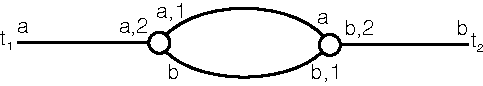
\includegraphics[width=0.5\textwidth]{resources/chap_feyn_diag/4_3_feyn_diag.pdf}
		\caption{Labeled Feynman diagram.}
		\label{fig:labeled_feyn} 
	\end{figure}
	
	The expectation
	\begin{equation}
		\contraction[5ex]{\Big \langle \frac{(-i)^2}{3!}\int d\tau }{a}{(\tau)a(\tau)b(\tau)\int d\tau a(\tau)a(\tau)b(\tau)\int d\tau a(\tau)a(\tau)b(\tau)\int d\tau a(\tau)b(\tau)b(\tau)}{a}
		\contraction[3ex]{\Big \langle \frac{(-i)^2}{3!}\int d\tau a(\tau)}{a}{(\tau)b(\tau)\int d\tau }{a}
		\contraction[3.5ex]{\Big \langle \frac{(-i)^2}{3!}\int d\tau a(\tau)a(\tau)}{b}{(\tau)\int d\tau a(\tau)a(\tau)b(\tau)\int d\tau a(\tau)a(\tau)}{b}
		\contraction[2ex]{\Big \langle \frac{(-i)^2}{3!}\int d\tau a(\tau)a(\tau)b(\tau)\int d\tau a(\tau)}{a}{(\tau)b(\tau)\int d\tau }{a}
		\contraction[2.5ex]{\Big \langle \frac{(-i)^2}{3!}\int d\tau a(\tau)a(\tau)b(\tau)\int d\tau a(\tau)a(\tau)}{b}{(\tau)\int d\tau a(\tau)a(\tau)b(\tau)\int d\tau a(\tau)}{b}
		\contraction[2ex]{\Big \langle \frac{(-i)^2}{3!}\int d\tau a(\tau)a(\tau)b(\tau)\int d\tau a(\tau)a(\tau)b(\tau)\int d\tau a(\tau)}{a}{(\tau)b(\tau)\int d\tau }{a}
		\contraction[1.5ex]{\Big \langle \frac{(-i)^2}{3!}\int d\tau a(\tau)a(\tau)b(\tau)\int d\tau a(\tau)a(\tau)b(\tau)\int d\tau a(\tau)a(\tau)b(\tau)\int d\tau a(\tau)b(\tau)}{b}{(\tau)a(t_1)}{b}
		\Big \langle \frac{(-i)^2}{3!}\int d\tau a(\tau)a(\tau)b(\tau)\int d\tau a(\tau)a(\tau)b(\tau)\int d\tau a(\tau)a(\tau)b(\tau)\int d\tau a(\tau)b(\tau)b(\tau)a(t_1)b(t_2)\Big \rangle
	\end{equation} 
	 is mapped to labeled Feynman diagram in Fig. \ref{fig:labeled_feyn2}.
	
	\begin{figure}[htb]
		\centering  
		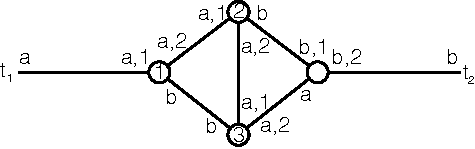
\includegraphics[width=0.5\textwidth]{resources/chap_feyn_diag/4_3_feyn_diag2.pdf}
		\caption{Another labeled Feynman diagram.}
		\label{fig:labeled_feyn2} 
	\end{figure}
	
	If we drop the label of order, we get the commonly known Feynman diagram. For example, the labeled Feynman diagram in Fig. \ref{fig:labeled_feyn2} becomes the diagram in Fig. \ref{fig:unlabeled_feyn3}. If we use different type of line (with an optional arrow) in the diagram to identify different type of propogator, we may even drop the label of type, and get the most concise form of Feynman diagram shown in Fig. \ref{fig:unlabeled_feyn4}.
	
	\begin{figure}[htb]
		\centering  
		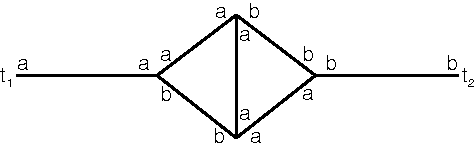
\includegraphics[width=0.5\textwidth]{resources/chap_feyn_diag/4_3_feyn_diag3.pdf}
		\caption{Unlabeled Feynman diagram.}
		\label{fig:unlabeled_feyn3} 
	\end{figure}
	
	\begin{figure}[htb]
		\centering  
		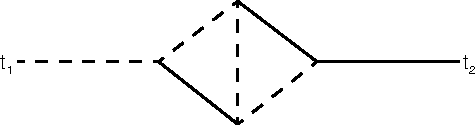
\includegraphics[width=0.5\textwidth]{resources/chap_feyn_diag/4_3_feyn_diag4.pdf}
		\caption{Feynman diagram in concise form, with solid line between b and b and dashed line between a and a.}
		\label{fig:unlabeled_feyn4} 
	\end{figure}
	
	It's easy to prove that there's a 1-1 correspondence of labeled Feynman diagram and full Wick contraction. But different Wick contractions may give the same unlabeled Feynman diagrams. We will prove that different Wick contractions that give the same unlabeled Feynman diagram give the same result. We will calculate the multiplicity of Wick contractions that give the same unlabeled Feynman diagram. First we have
	\begin{theorem}
		Let A and B be two different labeled Feynman diagram that gives the same unlabeled Feynman diagram. Then A can be transformed into B by composite of:
		\begin{itemize}
			\item Permutation of the order of identical vertexes.
			\item Internal symmetry action of each vertex.
		\end{itemize} 
	\end{theorem}
	\begin{proof}
		Obvious.
	\end{proof}
	
	\begin{theorem}
		Let A and B be two different full Wick contractions that gives the same unlabeled Feynman diagram. Then A have the same value.
	\end{theorem}
	\begin{proof}
		From last theorem we know A can be transformed into B by composite of:
		\begin{itemize}
			\item Permutation of interaction terms.
			\item Internal symmetry action of each interaction term.
		\end{itemize} 
		From definition of Wick contraction, it's easy to see that commuting operators will generate a phase factor in the natural way. Since interaction terms is bosonic operator (due to superselection law), the first operation will generate no phase factor. Since there is no identical fermionic operators inside a vertex due to Pauli's exclusion principle, the second operation will also generate no phase factor.
	\end{proof}
	
	The operations talked above forms a group that acts on the space of labeled Feynman diagrams. So the multiplicity of each unlabeled Feynman diagram is the order of the orbit that equals
	\begin{equation}
		\frac{|G|}{|S|}=\frac{\prod_i n_i!|G_i|^{n_i}}{\rm symmetric\ factor}
	\end{equation}
	where $n_i$ is the repetition of the interaction term $i$ and $G_i$ is the internal symmetry group of the interaction term $i$. The order of stabilizer S of the action is also called symmetric factor. It can be defined as: the number of operations that leave the labeled Feynman diagrams invariant.
	
	From now on, by saying Feynman diagrams, we mean unlabeled Feynman diagrams (in concise form if possible).
	
	First we write a general local interaction Hamiltonian as
	\begin{equation}
		H_{int}(t)=\sum_i \frac {g_i}{|G_i|} H_{int}^{[i]}(t)
	\end{equation}
	
	Our purpose is to calculate
	\begin{equation}
		\sum_n\Big \langle T\Big[\frac{(-i)^n}{n!}\Big[\int dt H_{int}^{[i]}(t)\Big]^nO_1(x_1)\cdots O_n(x_n)\Big] \Big \rangle \label{eqn:green_full}
	\end{equation} 
	
	As we have discussed, we may only calculate
	\begin{equation}
		\Big \langle T\Big[ \prod_i\frac 1{n_i!}\Big[-i\int dt \frac {g_i}{|G_i|} H_{int}^{[i]}(t)\Big]^{n_i}O_1(t_1)\cdots O_n(t_n)\Big] \Big \rangle \label{eqn:green_part}
	\end{equation} 
	
	We define the value of a Feynman diagram as the sum of all full Wick contractions in Eqn. \ref{eqn:green_full} to give the  Feynman diagram. Eqn. \ref{eqn:green_full} is the sum of Eqn. \ref{eqn:green_part}. Obviously, each Feynman diagram only comes from a specific set of $\{n_i\}$. So the value of a Feynman diagram is just sum of all full Wick contractions in Eqn. \ref{eqn:green_part} with the specific set of $\{n_i\}$. We denote by M the full wick contraction of   
	\begin{equation}
		\Big \langle T\Big[\prod_i\Big[-i\int dt g_iH_{int}^{[i]}(t)\Big]^{n_i}O_1(t_1)\cdots O_n(t_n)\Big] \Big \rangle \label{eqn:green_part}
	\end{equation} 
	that gives the chosen Feynman diagram.
	
	It's easy to see any full wick contraction of \ref{eqn:green_part} that gives the chosen Feynman diagram is
	\begin{equation}
		\frac M{\prod_in_i!|G_i|^{n_i}} 
	\end{equation} 
	
	Multiply with the multiplicity we derived, we finally know that the value of a Feynman diagram is
	\begin{equation}
		\frac M{\rm symmetric\ factor} 
	\end{equation} 
	
	It's easy to see that Eqn. \ref{eqn:green_full} is the sum value of all Feynman diagrams. Obviously we can calculate the symmetric factor purely from the Feynman diagrams. If we can devise a method to calculate M purely from the Feynman diagrams, we can forget everything of: interaction picture, Gell-Mann-Low thm, Wick theorem and so on, and calculate the Green's function purely from Feynman diagrams.
	
	
	\section{Feynman Rule}
	
	The Feynman rule is set of rules to translate from a Feynman diagram to an equation, whose value is the $M$ we introduced in the last section.
	
	From Wick's theorem, we can translate a propagator to a two point Green's function. The rule is: 
	\begin{itemize}
		\item The type of the Green's functions is determined by the types of operators at two ends of the propagator.
		\item The first time parameter of the Green's function is time at the starting end (vertex has a dummy time variable to be integrated later). We may choose either end to be the starting end if the propagator is not directed.
		\item The second time  parameter of the Green's function is time at the ending end.
	\end{itemize}
	With these two point Green's functions, we may get M by adding $-ig_i$ and taking integrals on dummy time at each vertex (i determined by vertex type). However an overall phase factor $\pm 1$ generating from the permutation of the operators is left unknown. In case of bosons, the overall phase is just 1. In case of Majorana fermions, we refer to \cite{Majorana_rule}. Here we consider the situation that some operators are Dirac fermions. 	
	\subsection{Overall Phase Factor of Dirac Fermions}
	It's reasonable to assume that for each Dirac operator $a$ there's only one type of Dirac operator $b$ such that
	\begin{equation}
		G_{ab}(t_1,t_2)\neq0
	\end{equation}
	
	We may label b as $\bar{a}$ (or possibly its derivatives). Furthermore, it's crucial to see that Dirac fermionic operators come in pairs in each interaction term at the same time. So in a Feynmann diagram,  Dirac fermionic lines form several paths. Each path starts and ends at free ends of the diagram, or forms a loop. There's no bifurcation along the path.
	
	We consider a full contraction of
	\begin{equation}
		\prod_i\Big[-i\int dt g_iH_{int}^{[i]}(t)\Big]^{n_i}\psi(t_1)\psi(t_2)\cdots \bar\psi(t_n)
	\end{equation}
	
	Let the interaction term be $H_{int}^{[i]}=\bar\psi\psi\cdots$. 
	
	After necessary permutation of the interaction terms, a fermionic loop corresponds to
	\begin{equation}
		\contraction[1.5ex]{\cdots}{\bar\psi}{\psi\bar\psi\psi\cdots\bar\psi}{\psi}
		\contraction[1ex]{\cdots\bar\psi}{\bar\psi}{}{\bar\psi}
		\contraction[1ex]{\cdots\bar\psi\psi\bar\psi}{\bar\psi}{}{\psi}
		\contraction[1ex]{\cdots\bar\psi\psi\bar\psi\quad\,\,\,}{\bar\psi}{}{\bar\psi}
		\cdots\bar\psi\psi\bar\psi\psi\cdots\bar\psi\psi\cdots
	\end{equation}
	This gives a contribution of $-1$ factor.
	
	Then we consider the contribution of fermionic paths. We may drop all the fermionic loops.
	
	After necessary permutation of the interaction terms, a fermionic path with two ends $\psi(t_i)$ and $\bar\psi(t_j)$ corresponds to
	\begin{equation}
		\contraction[1.5ex]{\cdots}{\bar\psi}{\psi\bar\psi\psi\cdots\bar\psi\psi\cdots}{\psi}
		\contraction[1ex]{\cdots\bar\psi}{\bar\psi}{}{\bar\psi}
		\contraction[1ex]{\cdots\bar\psi\psi\bar\psi}{\bar\psi}{}{\psi}
		\contraction[1ex]{\cdots\bar\psi\psi\bar\psi\quad\,\,\,}{\bar\psi}{}{\bar\psi}
		\contraction[1ex]{\cdots\bar\psi\psi\bar\psi\psi\cdots\bar\psi}{\bar\psi}{\cdots\psi(t_i)\cdots}{\bar\psi}
		\cdots\bar\psi\psi\bar\psi\psi\cdots\bar\psi\psi\cdots\psi(t_i)\cdots\bar\psi(t_j)\cdots
	\end{equation}
	
	We can move the involved interaction part to the right of $\psi(t_i)$, becoming
	\begin{equation}
		\contraction[1ex]{\langle T[\cdots}{\bar\psi}{(t_i)}{\bar\psi}
		\contraction[1ex]{\langle T[\cdots\psi(t_i)\bar\psi}{\bar\psi}{}{\bar\psi}
		\contraction[1ex]{\langle T[\cdots\psi(t_i)\bar\psi\psi\bar\psi}{\bar\psi}{}{\psi}
		\contraction[1ex]{\langle T[\cdots\psi(t_i)\bar\psi\psi\bar\psi\quad\,\,\,}{\bar\psi}{}{\bar\psi}
		\contraction[1ex]{\langle T[\cdots\psi(t_i)\bar\psi\psi\bar\psi\psi\cdots\bar\psi}{\bar\psi}{\cdots}{\bar\psi}
		\langle T[\cdots\psi(t_i)\bar\psi\psi\bar\psi\psi\cdots\bar\psi\psi\cdots\bar\psi(t_j)\cdots]\rangle
	\end{equation}
	
	Let's take a closer look at this contraction. We may drop or the intermediate operators, and contract $\psi(t_i)$ and $\bar\psi(t_j)$ directly. This action will cause no extra sign. Let's do this operation for all fermionic paths, and drop all bosonic operators. We result in a full contraction of
	\begin{equation}
		\psi(t_1)\psi(t_2)\cdots \bar\psi(t_n)
	\end{equation}
	
	The sign contribution of all fermionic paths of the original full contraction is just the sign of this simplified full contraction.
	
	In conclusion
	\begin{enumerate}
		\item A fermionic loop gives a $-1$ factor.
		\item All fermionic paths gives the same factor as the simplified full contraction. Especially, if there's only two free ends, the fermionic paths gives no extra factor.
	\end{enumerate}
	
	\subsection{Feynman Rule, an Example}
	
	Let's consider a system with Lagragian
	\begin{equation}
		L=L_0-\int d^3{\bf x}U({\bf x})\bar\psi(x)\psi(x)-\frac 12\int d^3{\bf x}d^3{\bf x'}V({\bf x}-{\bf x'})\bar\psi(x)\bar\psi(x')\psi(x')\psi(x)-\int d^3{\bf x} g({\bf x}-{\bf x'})\bar\psi(x)\psi(x)\phi(x')
	\end{equation}
	where
	\begin{equation}
		L_0=\int dx(\bar\psi(x)\partial_0\psi(x)-\frac 1{2m}\partial_i\bar\psi(x)\partial_i\psi(x)-\mu\bar\psi(x)\psi(x))+\int dx(\frac 12(\partial_0\phi(x))^2-\frac 12 M_{ij}(x)\partial_i\phi(x)\partial_j\phi(x))
	\end{equation}
	is the free Lagragian of electrons and phonons. Coulomb interaction and electron-phonon interaction is considered.
	
	The space-time Feynmann rule is given in Tab. \ref{tab:space_frule}.
	
	\begin{table}[htp!]
		\centering
		\begin{tabular}{| >{\centering\arraybackslash}m{15em}|>{\centering\arraybackslash} m{12em}|}
		\hline
		\vspace{0.5ex}Component\vspace{0.5ex}&\vspace{0.5ex}Rule\vspace{0.5ex}\\
		\hline
		\vspace{2.5ex}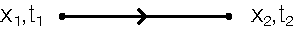
\includegraphics[scale=1]{resources/chap_feyn_diag/fdiag_frule1.pdf}\vspace{1ex}&$iG(x_2-x_1,t_2-t_1)$\vspace{0.5ex}\\
		\hline
		\vspace{2.5ex}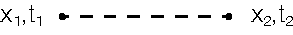
\includegraphics[scale=1]{resources/chap_feyn_diag/fdiag_frule2.pdf}\vspace{1ex}&$iD(x_2-x_1,t_2-t_1)$\vspace{0.5ex}\\
		\hline
		\vspace{2.5ex}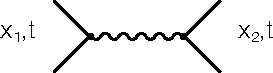
\includegraphics[scale=1]{resources/chap_feyn_diag/fdiag_frule3.pdf}\vspace{1ex}&$-i\int dtdx_1dx_2V(x_1-x_2)$\vspace{0.5ex}\\
		\hline
		\vspace{2.5ex}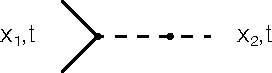
\includegraphics[scale=1]{resources/chap_feyn_diag/fdiag_frule4.pdf}\vspace{1ex}&$-i\int dtdx_1dx_2g(x_1-x_2)$\vspace{0.5ex}\\
		\hline
		\vspace{2.5ex}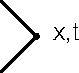
\includegraphics[scale=1]{resources/chap_feyn_diag/fdiag_frule5.pdf}\vspace{1ex}&$-i\int dtdxU(x)$\vspace{0.5ex}\\
		\hline
		\vspace{2.5ex}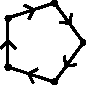
\includegraphics[scale=1]{resources/chap_feyn_diag/fdiag_frule6.pdf}\vspace{1ex}&$(-1)\cdot(2S+1)$\vspace{0.5ex}\\
		\hline
		\end{tabular}
		\caption{Space-time Feynmann rule for fermion-phonon system at zero temperature.}
		\label{tab:space_frule}
	\end{table}
	
	We can transform the Feynmann rule into momentum-energy space.
	
	For each propogator we have
	\begin{equation}
		G(x-y)=\int\frac {d^4p}{(2\pi)^4}e^{ip\cdot(x-y)}G(p)
	\end{equation}
	where $p$ is directed from $y$-vertex to $x$-vertex, and the we choose the Minkowski metric $(-1,1,1,1)$.
	
	For Coulomb interaction vertex we have
	\begin{equation}
		\int dt\int d^3{\bf x}d^3{\bf y}V({\bf x}-{\bf y})=\int dt\int d^3{\bf x}d^3{\bf y}\int\frac{d^3{\bf q}}{(2\pi)^3}e^{i{\bf q}\cdot({\bf x}-{\bf y})}V({\bf q})
	\end{equation}
	where $q$ is directed from $y$-vertex to $x$-vertex.
	
	For  potential vertex we have
	\begin{equation}
		\int d^4xU({\bf x})=\int d^4x\int\frac{d^3{\bf q}}{(2\pi)^3}e^{i{\bf q}\cdot {\bf x}}U({\bf q})
	\end{equation}
	where $q$ is directed inwards.
	
	For electron-phonon interaction vertex we have
	\begin{equation}
		\int dt\int d^3{\bf x}d^3{\bf y}g({\bf x}-{\bf y})=\int dt\int d^3{\bf x}d^3{\bf y}\int\frac{d^3{\bf q}}{(2\pi)^3}e^{i{\bf q}\cdot({\bf x}-{\bf y})}g({\bf q})
	\end{equation}
	where $q$ is directed from $y$-vertex to $x$-vertex.
	
	Finally we have many
	\begin{equation}
		\int d^4xe^{i\sum_i\pm p_i\cdot x}=(2\pi)^4\delta(\sum_i\pm p_i)
	\end{equation}
	where $\pm$ is for the inwards/outwards momentum direction. This ensures the conservation of the momentum. We do such integral on interaction vertex. So on each free end, there's a $e^{ip\cdot x_i}$ left. This will result in $(2\pi)^4\delta(p_i-p)$ after Fourier transformation of the whole thing.
	
	Another thing to notice is that to keep the order of the interaction term unchanged under time-ordering, we should modify the interaction term into
	\begin{eqnarray}
		&&\int d^3{\bf x}U({\bf x})\bar\psi({\bf x},t+\delta)\psi({\bf x},t)-\frac 12\int d^3{\bf x}d^3{\bf x'}V({\bf x}-{\bf x'})\bar\psi({\bf x},t+3\delta)\bar\psi({\bf x'},t+2\delta)\psi({\bf x'},t+\delta)\psi({\bf x},t)\nonumber\\
		&&-\int d^3{\bf x} g({\bf x}-{\bf x'})\bar\psi({\bf x},t+\delta)\psi({\bf x},t)\phi({\bf x'},t)
	\end{eqnarray}
	This leads to some $e^{i\delta E}$ factor in momentum-energy Feynmann rule.
	
	The momentum-energy Feynmann rule is given in Tab. \ref{tab:momentum_frule}.
	
	\begin{table}[htp!]
		\centering
		\begin{tabular}{| >{\centering\arraybackslash}m{15em}|>{\centering\arraybackslash} m{24em}|}
		\hline
		\vspace{0.5ex}Component\vspace{0.5ex}&\vspace{0.5ex}Rule\vspace{0.5ex}\\
		\hline
		\vspace{2.5ex}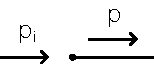
\includegraphics[scale=1]{resources/chap_feyn_diag/fdiag_frulep6.pdf}\vspace{1ex}&$(2\pi)^4\delta(p_i-p)$\vspace{0.5ex}\\
		\hline
		\vspace{2.5ex}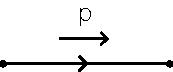
\includegraphics[scale=1]{resources/chap_feyn_diag/fdiag_frulep1.pdf}\vspace{1ex}&$i\int\frac{d^4p}{(2\pi)^4}G(p)$\vspace{0.5ex}\\
		\hline
		\vspace{2.5ex}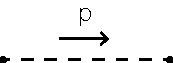
\includegraphics[scale=1]{resources/chap_feyn_diag/fdiag_frulep2.pdf}\vspace{1ex}&$i\int\frac{d^4p}{(2\pi)^4}D(p)$\vspace{0.5ex}\\
		\hline
		\vspace{2.5ex}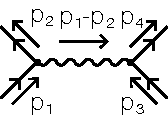
\includegraphics[scale=1]{resources/chap_feyn_diag/fdiag_frulep3.pdf}\vspace{1ex}&$-iV({\bf p_1}-{\bf p_2})(2\pi)^4\delta^4(p_1-p_2+p_3-p_4)e^{-i\delta E_3}e^{i2\delta E_4}e^{i3\delta E_2}$\vspace{0.5ex}\\
		\hline
		\vspace{2.5ex}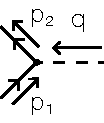
\includegraphics[scale=1]{resources/chap_feyn_diag/fdiag_frulep4.pdf}\vspace{1ex}&$-ig({\bf q})(2\pi)^4\delta(p_1-p_2+q)e^{i\delta E_2}$\vspace{0.5ex}\\
		\hline
		\vspace{2.5ex}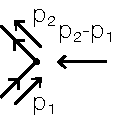
\includegraphics[scale=1]{resources/chap_feyn_diag/fdiag_frulep5.pdf}\vspace{1ex}&$-iU({\bf p_2}-{\bf p_1})(2\pi)\delta(E_2-E_1)e^{i\delta E_2}$\vspace{0.5ex}\\
		\hline
		\vspace{2.5ex}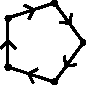
\includegraphics[scale=1]{resources/chap_feyn_diag/fdiag_frule6.pdf}\vspace{1ex}&$(-1)\cdot(2S+1)$\vspace{0.5ex}\\
		\hline
		\end{tabular}
		\caption{Momentum-energy Feynmann rule for fermion-phonon system at zero temperature.}
		\label{tab:momentum_frule}
	\end{table}
	
	Similarly, at finite temperature, we have the Feynmann rule for Matsubara Green's function. The space-time Feynmann rule is given in Tab. \ref{tab:space_frule_ft}. And the momentum-energy Feynmann rule is given in Tab. \ref{tab:momentum_frule_fT}.
	
	\begin{table}[htp!]
		\centering
		\begin{tabular}{| >{\centering\arraybackslash}m{15em}|>{\centering\arraybackslash} m{12em}|}
		\hline
		\vspace{0.5ex}Component\vspace{0.5ex}&\vspace{0.5ex}Rule\vspace{0.5ex}\\
		\hline
		\vspace{2.5ex}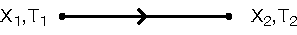
\includegraphics[scale=1]{resources/chap_feyn_diag/fdiag_fruleT1.pdf}\vspace{1ex}&$-\mathcal G(x_2-x_1,t_2-t_1)$\vspace{0.5ex}\\
		\hline
		\vspace{2.5ex}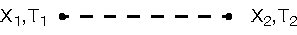
\includegraphics[scale=1]{resources/chap_feyn_diag/fdiag_fruleT2.pdf}\vspace{1ex}&$-\mathcal D(x_2-x_1,t_2-t_1)$\vspace{0.5ex}\\
		\hline
		\vspace{2.5ex}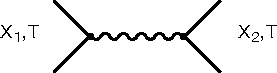
\includegraphics[scale=1]{resources/chap_feyn_diag/fdiag_fruleT3.pdf}\vspace{1ex}&$-\int d\tau dx_1dx_2V(x_1-x_2)$\vspace{0.5ex}\\
		\hline
		\vspace{2.5ex}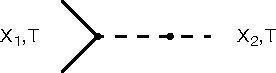
\includegraphics[scale=1]{resources/chap_feyn_diag/fdiag_fruleT4.pdf}\vspace{1ex}&$-\int d\tau dx_1dx_2g(x_1-x_2)$\vspace{0.5ex}\\
		\hline
		\vspace{2.5ex}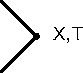
\includegraphics[scale=1]{resources/chap_feyn_diag/fdiag_fruleT5.pdf}\vspace{1ex}&$-\int d\tau dxU(x)$\vspace{0.5ex}\\
		\hline
		\vspace{2.5ex}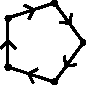
\includegraphics[scale=1]{resources/chap_feyn_diag/fdiag_frule6.pdf}\vspace{1ex}&$(-1)\cdot(2S+1)$\vspace{0.5ex}\\
		\hline
		\end{tabular}
		\caption{Space-time Feynmann rule for fermion-phonon system at finite temperature.}
		\label{tab:space_frule_ft}
	\end{table}
	
	\begin{table}[htp!]
		\centering
		\begin{tabular}{| >{\centering\arraybackslash}m{15em}|>{\centering\arraybackslash} m{24em}|}
		\hline
		\vspace{0.5ex}Component\vspace{0.5ex}&\vspace{0.5ex}Rule\vspace{0.5ex}\\
		\hline
		\vspace{2.5ex}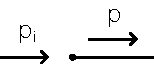
\includegraphics[scale=1]{resources/chap_feyn_diag/fdiag_frulep6.pdf}\vspace{1ex}&$(2\pi)^3\delta({\bf p_i}-{\bf p})\delta_{\omega_{i,n}-\omega_n}$\vspace{0.5ex}\\
		\hline
		\vspace{2.5ex}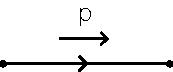
\includegraphics[scale=1]{resources/chap_feyn_diag/fdiag_frulep1.pdf}\vspace{1ex}&$-\int\frac{d^3p}{(2\pi)^3}\sum_n \frac1\beta\mathcal G({\bf p},i\omega_n)$\vspace{0.5ex}\\
		\hline
		\vspace{2.5ex}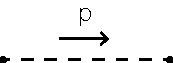
\includegraphics[scale=1]{resources/chap_feyn_diag/fdiag_frulep2.pdf}\vspace{1ex}&$-\int\frac{d^3p}{(2\pi)^3}\sum_n \frac1\beta\mathcal D({\bf p},i\omega_n)$\vspace{0.5ex}\\
		\hline
		\vspace{2.5ex}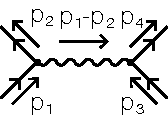
\includegraphics[scale=1]{resources/chap_feyn_diag/fdiag_frulep3.pdf}\vspace{1ex}&$-V({\bf p_1}-{\bf p_2})(2\pi)^3\delta^3({\bf p_1}-{\bf p_2}+{\bf p_3}-{\bf p_4})$\newline$\beta\delta_{\omega_{n_1}-\omega_{n_2}+\omega_{n_3}-\omega_{n_4}}e^{-i\delta \omega_{n_3}}e^{i2\delta \omega_{n_4}}e^{i3\delta \omega_{n_2}}$\vspace{0.5ex}\\
		\hline
		\vspace{2.5ex}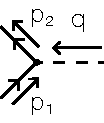
\includegraphics[scale=1]{resources/chap_feyn_diag/fdiag_frulep4.pdf}\vspace{1ex}&$-g({\bf q})(2\pi)^3\delta({\bf p_1}-{\bf p_2}+{\bf q})\beta\delta_{\omega_{n_1}-\omega_{n_2}+\nu_n}e^{i\delta \omega_{n_2}}$\vspace{0.5ex}\\
		\hline
		\vspace{2.5ex}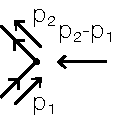
\includegraphics[scale=1]{resources/chap_feyn_diag/fdiag_frulep5.pdf}\vspace{1ex}&$-U({\bf p_2}-{\bf p_1})\beta\delta_{\omega_{n_2}-\omega_{n_1}}e^{i\delta \omega_{n_2}}$\vspace{0.5ex}\\
		\hline
		\vspace{2.5ex}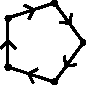
\includegraphics[scale=1]{resources/chap_feyn_diag/fdiag_frule6.pdf}\vspace{1ex}&$(-1)\cdot(2S+1)$\vspace{0.5ex}\\
		\hline
		\end{tabular}
		\caption{Momentum-energy Feynmann rule for fermion-phonon system at finite temperature.}
		\label{tab:momentum_frule_fT}
	\end{table}


	\section{Cancelation of Vacuum Diagrams}
	\begin{equation}
		\langle T[\prod_nO_H(t_n)]\rangle=\frac{\sum{\rm diagrams\ with\ ends\ }O(t_1)\cdots O(t_n)}{\sum{\rm diagrams\ with\ no\ ends}}
	\end{equation}
	
	A Feynmann diagram with no ends is also called a vacuum diagram.
	
	Let's label the connected vacuum diagrams by $V_i$. Each vacuum diagram can be uniquely labeled by a series $(n_i)$, indicating that the diagram contains $n_i$ $V_i$s. The symmetrical factor of the vacuum diagram labeled by $(n_i)$ is
	\begin{equation}
		\prod_i n_i!S_i^{n_i}
	\end{equation}
	where $S_i$ is the symmetrical factor of $V_i$.
	
	Let $F_i$ be the value of $V_i$ and let $\tilde F_i$ be the value of $V_i$ with the symmetrical value not divided. Then the value of the vacuum diagram labeled by $(n_i)$ is
	\begin{equation}
		F_{(n_i)}=\frac{\prod_i \tilde F_i^{n_i}}{\prod_i n_i!S_i^{n_i}}=\prod_i \frac{ F_i^{n_i}}{n_i!}
	\end{equation}
	
	So
	\begin{eqnarray}
		\sum{\rm vacuum\ diagrams}&=&\sum_{(n_i)}\prod_i\frac{ F_i^{n_i}}{n_i!}\\
		&=&\prod_i\sum_{n_i} \frac{ F_i^{n_i}}{n_i!}\\
		&=&\prod_ie^{ F_i}\\
		&=&e^{\sum_i F_i}\\
		&=&e^{\sum{\rm connected\ vacuum\ diagrams}}
	\end{eqnarray}
	
	Similarly
	\begin{eqnarray}
		\sum{\rm diagrams\ with\ ends\ }O(t_1)\cdots O(t_n)&=&\sum{\rm connected\  diagrams\ with\ ends\ }O(t_1)\cdots O(t_n)\cdot\nonumber\\
		&&e^{\sum{\rm connected\ vacuum\ diagrams}}
	\end{eqnarray}
	
	By connected diagrams with ends $O(t_1)\cdots O(t_n)$, we mean each component of the diagram is connected to at least one of the ends. Although the diagram may not be connected.
	
	So
	\begin{equation}
		\langle T[\prod_nO_H(t_n)]\rangle=\sum {\rm connected\ diagrams\ with\ ends\ }O(t_1)\cdots O(t_n)
	\end{equation}
	
	\section{Linked-cluster Theorem}
	When $T=0$, since
	\begin{equation}
		\Delta E=\lim_{T\rightarrow\infty}\frac i{2T}\ln\langle 0|S_H(-T\rightarrow T)|0\rangle
	\end{equation}
	
	We have
	\begin{eqnarray}
		\frac{\Delta E}V&=&\frac i{2VT}\ln\sum{\rm vacuum\ diagrams}\\
		&=&\frac i{2VT}\sum{\rm connected\ vacuum\ diagrams}
	\end{eqnarray}
	
	So connected vacuum diagrams per space-time volume is the density of the interaction energy.
	
	At finite temperature, we have
	\begin{eqnarray}
		-\Delta F&=&\ln\Tr[e^{-\beta H}]-\ln\Tr[e^{-\beta H_0}]\\
		&=&\ln\Tr\langle e^{\beta H_0}e^{-\beta H}\rangle_0\\
		&=&\ln\Tr\langle S(0\rightarrow\beta)\rangle_0\\
		&=&\ln\sum{\rm vacuum\ diagrams}\\
		&=&\sum{\rm connected\ vacuum\ diagrams}
	\end{eqnarray}
	
	So
	\begin{equation}
		\frac{\Delta F}{V}=\frac {-1}{V\beta}\sum{\rm connected\ vacuum\ diagrams}
	\end{equation}
	
\chapter{Linear Response Theory and Dissipation-Fluctuation Theorem}

\section{Linear Response Theory}

We consider a system coupling to external field $f(x,t)$. Let the Hamiltonian be
\begin{equation}
	H(t)=H_0+H_{cp}(t)=H_0-\int dxA(x)f(x,t)
\end{equation}
Here we use $H_0$ to denote the interaction system with no external field. We treat $H_0$ as a free Hamiltonian and $H_{cp}(t)$ as the interaction term.

We assume the external field to vanish in the infinite past. Then
\begin{equation}
	|\Omega(0)\rangle=e^{i\phi}S(0,-\infty)|0\rangle
\end{equation} 

So
\begin{eqnarray}
	\langle \Omega|A_H(x,t)|\Omega\rangle&=&\langle 0|S(-\infty,0)A_H(x,t)S(0,-\infty)|0\rangle\\
	&=&\langle 0|S(-\infty,t)A_I(x,t)S(t,-\infty)|0\rangle\\
	&\simeq&\langle 0|A_I(x,t)-i\int_{-\infty}^tdt'[A_I(x,t),H_{cp,I}(t')]|0\rangle\\
	&=&\langle 0|A_I(x,t)+i\int_{-\infty}^tdt'[A_I(x,t),\int dx'A_I(x',t')f(x',t')]|0\rangle
\end{eqnarray}

So
\begin{equation}
	\langle \Omega|\Delta A_H(x,t)|\Omega\rangle=i\int_{-\infty}^tdt'\int dx'\langle0|[\Delta A_I(x,t),\Delta A_I(x',t')]|0\rangle f(x',t')
\end{equation}
where $\Delta A(x,t)=A(x,t)-\langle 0|A_I(x,t)|0\rangle$.

Define
\begin{equation}
	\chi(x-x',t-t')=i\langle0|[\Delta A_I(x,t),\Delta A_I(x',t')]|0\rangle\theta(t-t')
\end{equation}

Then
\begin{equation}
	\Delta A(x,t)=\langle \Omega|\Delta A_H(x,t)|\Omega\rangle=i\int dt'dx'\chi(x-x',t-t')f(x',t')
\end{equation}

In momentum space
\begin{equation}
	\Delta A(p)=\chi(p)f(p)
\end{equation}

Let's define
\begin{equation}
	\chi^T(x-x',t-t')=i\langle0|T[\Delta A_I(x,t)\Delta A_I(x',t')]|0\rangle
\end{equation}

As shown in Sect. \ref{sec:0t_green}, we have
\begin{equation}
	\chi({\bf p},\omega)=\chi^T({\bf p},\omega+i\delta)
\end{equation}

Now we return to our old familiar style. We continue to treat $H_0$ as an interacting Hamiltonian with ground state $|\Omega\rangle$. We can express $\chi^T(x-x',t-t')$ by Feynmann diagrams
\begin{eqnarray}
	-i\chi^T(x-x',t-t')&=&\langle\Omega|T[\Delta A(x,t)\Delta A(x',t')]|\Omega\rangle\\
	&=&\langle\Omega|T[A(x,t),A(x',t')]|\Omega\rangle-\langle\Omega|A(x,t)|\Omega\rangle\langle\Omega|A(x',t')|\Omega\rangle\\
	&=&\sum{\rm diagrams\ connected\ to\ }x{\rm\ or\ }x'-\sum{\rm diagrams\ connected\ to\ }x\nonumber\\
	&&\sum{\rm diagrams\ connected\ to\ }x'\\
	&=&\sum{\rm diagrams\ connected\ to\ }x{\rm\ and\ }x'\\
	&=&\adjustbox{raise=-2.8ex}{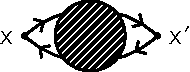
\includegraphics[scale=1]{resources/chap_linear_pesp/fdiagapp_20.pdf}}
\end{eqnarray}
One may check the correctness of the symmetrical factor.

\section{Linear Response at Finite Temperature}
At finite temperature, we study the density matrix in the interaction picture.
 
We assume the external field to vanish in the infinite past. Then
\begin{eqnarray}
	i\rho_I(t)&=&\int_{-\infty}^td\tau[H_{int,I}(\tau),\rho_I(\tau)]+\rho_I(-\infty)\\
	&=&\int_{-\infty}^td\tau[H_{int,I}(\tau),\rho_0]+\rho_0+\mathcal O(H_{int,I}^2)
\end{eqnarray}
where $\rho_0$ is the density matrix of the free system.

So
\begin{eqnarray}
	\langle A_H(x,t)\rangle&=&{\rm Tr}[A_I(x,t)\rho_I(t)]\\
	&=&-i{\rm Tr}[A_I(x,t)\int_{-\infty}^tdt'[H_{int,I}(t'),\rho_0]]+{\rm Tr}[A_I(t)\rho_0]\\
	&=&-i\int_{-\infty}^tdt'{\rm Tr}[[A_I(x,t),H_{int,I}(t')]\rho_0]+{\rm Tr}[A_I(t)\rho_0]\\
	&=&-i\int_{-\infty}^tdt'\langle[A_I(x,t),H_{int,I}(t')]\rangle_0+\langle A_I(t)\rangle_0\\
	&=&-i\int_{-\infty}^tdt'\langle[A_I(x,t),\int dx'A_I(x',t')f(x',t')]\rangle_0+\langle A_I(t)\rangle_0
\end{eqnarray}

So
\begin{equation}
	\langle\Delta A_H(x,t)\rangle=i\int_{-\infty}^tdt'\int dx'\langle[\Delta A_I(x,t),\Delta A_I(x',t')]\rangle_0 f(x',t')
\end{equation}
where $\Delta A(x,t)=A(x,t)-\langle A_I(x,t)\rangle_0$.

Define
\begin{equation}
	\chi(x-x',t-t')=i\langle[\Delta A_I(x,t),\Delta A_I(x',t')]\rangle_0\theta(t-t')
\end{equation}

Then
\begin{equation}
	\Delta A(x,t)=\langle\Delta A_H(x,t)\rangle=i\int dt'dx'\chi(x-x',t-t')f(x',t')
\end{equation}

In momentum space
\begin{equation}
	\Delta A(p)=\chi(p)f(p)
\end{equation}

Let's define
\begin{equation}
	\chi^M(x-x',\tau-\tau')=-\langle0|T[\Delta A_I(x,\tau)\Delta A_I(x',\tau')]|0\rangle
\end{equation}
where $\tau$ and $\tau'$ are imaginary time.

As shown in Sect. \ref{sec:greens_finiteT}, we have
\begin{equation}
	\chi({\bf p},\omega)=\chi^M({\bf p},i\omega_n\rightarrow\omega+i\delta)
\end{equation}

Now we return to our old familiar style. We continue to treat $H_0$ as an interacting Hamiltonian with ground state $|\Omega\rangle$. We can express $\chi^M(x-x',t-t')$ by Feynmann diagrams
\begin{eqnarray}
	-\chi^M(x-x',\tau-\tau')&=&\langle\Omega|T[\Delta A(x,\tau)\Delta A(x',\tau')]|\Omega\rangle\\
	&=&\langle\Omega|T[A(x,\tau),A(x',\tau')]|\Omega\rangle-\langle\Omega|A(x,\tau)|\Omega\rangle\langle\Omega|A(x',\tau')|\Omega\rangle\\
	&=&\sum{\rm diagrams\ connected\ to\ }x{\rm\ or\ }x'-\sum{\rm diagrams\ connected\ to\ }x\nonumber\\
	&&\sum{\rm diagrams\ connected\ to\ }x'\\
	&=&\sum{\rm diagrams\ connected\ to\ }x{\rm\ and\ }x'\\
	&=&\adjustbox{raise=-2.8ex}{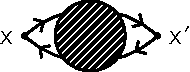
\includegraphics[scale=1]{resources/chap_linear_pesp/fdiagapp_20.pdf}}
\end{eqnarray}
One may check the correctness of the symmetrical factor.

\section{Dissipation-Fluctuation Theorem}
We define the correlation of to operators $A(x)$ and $A(x')$ to be
\begin{equation}
	S(x)=\langle\Delta A(x)\Delta A_2(x')\rangle
\end{equation}

When $T=0$, from Sect. \ref{sec:0t_green} we have

\begin{equation}
	S({\rm p},\omega)=2\theta(\omega)\Im\chi({\rm p},\omega)
\end{equation}

At finite temperature, from Sect. \ref{sec:greens_finiteT} we have

\begin{equation}
	S({\rm p},\omega)=\frac2{1-\eta e^{-\beta\omega}}\Im\chi({\rm p},\omega)
\end{equation}

These are the quantum dissipation-fluctuation theorem.
	
\chapter{Boson System}
	
\chapter{Fermion System}

\section{Hartee-Fock Approximation}

Let's consider a fermionic system with Coulomb interaction. 

\subsection{Interaction Energy}
To 1st order, interaction energy density is
\begin{eqnarray}
	\frac{\Delta E}V&=&\frac i{VT}\Bigg[\adjustbox{valign=c}{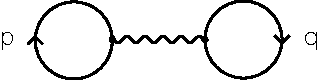
\includegraphics[scale=1]{resources/chap_ferm/fdiagapp_1.pdf}}\ -\ \adjustbox{valign=c}{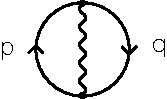
\includegraphics[scale=1]{resources/chap_ferm/fdiagapp_2.pdf}}\Bigg]\\
	&=&\frac {i(2\pi)^4\delta(0)}{VT}\frac 12\int \frac{d^4p}{(2\pi)^4}\frac{d^4q}{(2\pi)^4}e^{i(p_0+q_0)\delta}[(-(2S+1))^2(-iV(0))+\nonumber\\
	&& (-(2S+1))(-iV({\bf p}-{\bf q}))](iG(p))(iG(q))\\
	&=&\frac 12\int \frac{d^3{\bf p}}{(2\pi)^3}\frac{d^3{\bf q}}{(2\pi)^3}[(2S+1)^2V(0)-(2S+1)V({\bf p}-{\bf q})]f_{\bf p}f_{\bf q}
\end{eqnarray}
where
\begin{equation}
	f_{\bf p}=-i\int \frac{d\omega}{(2\pi)}e^{i\omega\delta}G(p)=-iG({\bf p},0^-)=-\langle T[c_{p}(t)c_{p}^\dagger(t+\delta)]\rangle=\langle c_{p}^\dagger c_{p}\rangle=\theta(\epsilon_F-\epsilon_{\bf p})
\end{equation}

The first term $\frac 12\int \frac{d^3{\bf p}}{(2\pi)^3}\frac{d^3{\bf q}}{(2\pi)^3}(2S+1)^2V(0)f_{\bf p}f_{\bf q}$ cancels with the positive charged background, as we'll show in Jellium model. So the interaction energy is
\begin{eqnarray}
	\frac{E_{int}}V&=&-\frac 12\int \frac{d^3{\bf p}}{(2\pi)^3}\frac{d^3{\bf q}}{(2\pi)^3}(2S+1)V({\bf p}-{\bf q})f_{\bf p}f_{\bf q}\\
	&=&-\frac 12\int_{|{\rm p}|,|{\rm q}|<k_F} \frac{d^3{\bf p}}{(2\pi)^3}\frac{d^3{\bf q}}{(2\pi)^3}(2S+1)\frac{e^2}{\epsilon_0(|{\rm p}-{\rm q}|^2)}\\
	&=&-\rho\frac 3{4\pi}\frac{e^2k_f}{4\pi\epsilon_0}
\end{eqnarray}
where $\rho=(2S+1)k_F^3/(6\pi^2)$ is the density of the electrons.

\subsection{Exchange Correlation}

Then let's consider the equal-time density correlation function
\begin{equation}
	C_{\sigma\sigma'}({\bf x}-{\bf x'})=\langle \Omega|:n_\sigma({\bf x})n_\sigma({\bf x'}):|\Omega\rangle
\end{equation}

It is related to the interaction energy by
\begin{equation}
	\Delta E=\langle \Omega|\frac 12\int d^3{\bf x}d^3{\bf x'}V({\bf x}-{\bf x'})\bar\psi(x)\bar\psi(x')\psi(x')\psi(x)|\Omega\rangle=\frac 12\sum_{\sigma,\sigma'}\int d^3{\bf x}d^3{\bf x'}V({\bf x}-{\bf x'})C_{\sigma\sigma'}({\bf x}-{\bf x'})
\end{equation}

As usual, we have to the 0th order
\begin{eqnarray}
	C_{\sigma\sigma'}({\bf x}-{\bf x'})&=&\langle \Omega|T[\bar\psi_\sigma({\bf x},t+3\delta)\bar\psi_{\sigma'}({\bf x'},t+2\delta)\psi_{\sigma'}({\bf x'},t+\delta)\psi_\sigma({\bf x},t)]|\Omega\rangle\\
	&=&\adjustbox{valign=c}{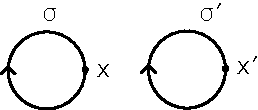
\includegraphics[scale=1]{resources/chap_ferm/fdiagapp_3.pdf}}\ +\ \adjustbox{valign=c}{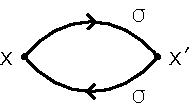
\includegraphics[scale=1]{resources/chap_ferm/fdiagapp_4.pdf}}\ \delta_{\sigma\sigma'}\\
	&=&((-1)\cdot iG(0,0^-))^2+(-1)\cdot iG({\bf x}-{\bf x'},0^-)\cdot iG({\bf x'}-{\bf x},0^-)\delta_{\sigma\sigma'}\\
	&=&\rho_0^2+G({\bf x}-{\bf x'},0^-)G({\bf x'}-{\bf x},0^-)\delta_{\sigma\sigma'}
\end{eqnarray}
where
\begin{equation}
	\rho_0=-iG(0,0^-)=-\langle T[c_{x}(t)c_{x}^\dagger(t+\delta)]\rangle=\langle c_{x}c_{x}\rangle=\frac{k_F^3}{6\pi^2}
\end{equation}

We have
\begin{eqnarray}
	G({\bf x}-{\bf x'},0^-)&=&i\int_{|{\bf p}|<k_F}\frac{d^3{\bf p}}{(2\pi)^3}e^{i{\bf p}\cdot({\bf x}-{\bf x'})}\\
	&=&\frac i{(2\pi)^2}\int_0^{k_F}dp_r\int_0^\pi d\theta p_r^2\sin\theta e^{ip_r|{\bf x}-{\bf x'}|\cos\theta}\\
	&=&\frac i{2\pi^2r^3}(\sin(k_Fr)-k_Fr\cos(k_Fr))\\
	&=&\frac {3i\rho_0}{(k_fr)^3}(\sin(k_Fr)-k_Fr\cos(k_Fr))
\end{eqnarray}
where $r=|{\bf x}-{\bf x'}|$ and ${\bf p}=(p_r\sin\theta\cos\phi,p_r\sin\theta\sin\phi,p_r\cos\theta)$, with ${\bf x}-{\bf x'}$ as the direction of the z-axis.

Finally
\begin{equation}
	C_{\sigma\sigma'}(r)=\rho_0^2[1-9\frac{(\sin(k_Fr)-k_Fr\cos(k_Fr))^2}{(k_fr)^6}\delta_{\sigma\sigma'}]
\end{equation}

The function between $C_{\sigma\sigma}/\rho_0^2$ and $k_Fr$ is plotted in Fig. \ref{fig:eqt_corr}. At $r=0$, $C_{\sigma\sigma}$ goes to 0 due to Pauli's exclusion principle.
	\begin{figure}[htb]
		\centering  
		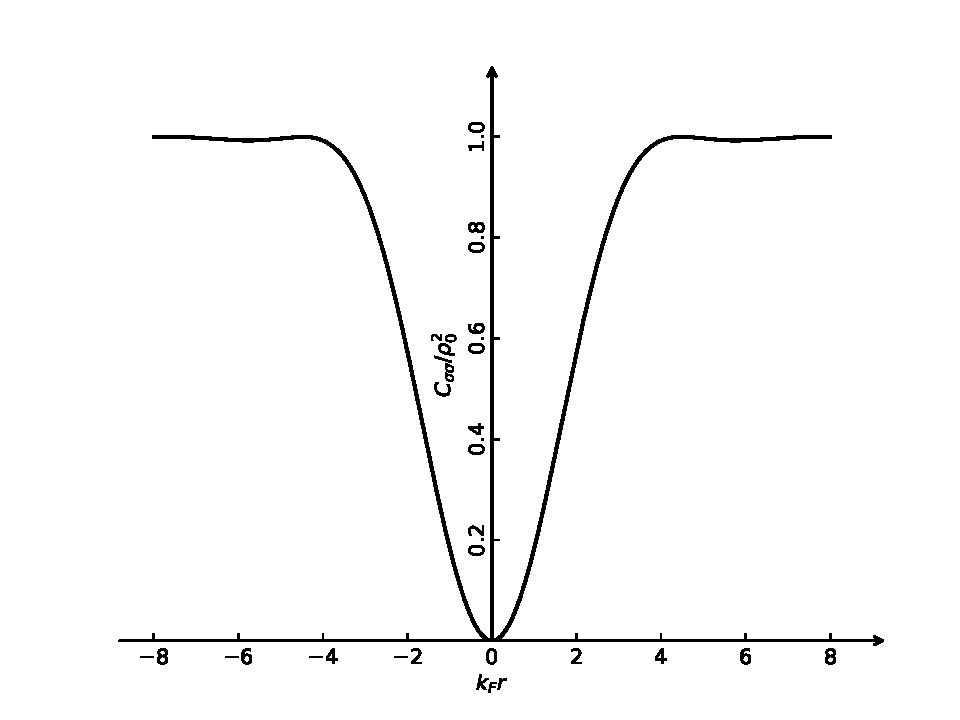
\includegraphics[width=0.8\textwidth]{resources/chap_ferm/fdiagapp_5.pdf}
		\caption{Equal-time density correlation function of the free electron system.}
		\label{fig:eqt_corr} 
	\end{figure}
	
\section{Potential Scattering}
	
Let's consider a fermionic system in an attractive potential $U(x)$. 

The Green's function is
\begin{eqnarray}
	iG(k,k')&=&\adjustbox{raise=-0.9ex}{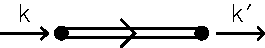
\includegraphics[scale=1]{resources/chap_ferm/fdiagapp_6.pdf}}\\
	&=& \adjustbox{raise=-0.9ex}{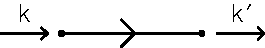
\includegraphics[scale=1]{resources/chap_ferm/fdiagapp_7.pdf}}+\adjustbox{raise=-6.1ex}{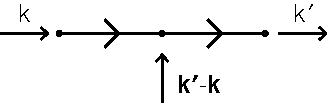
\includegraphics[scale=1]{resources/chap_ferm/fdiagapp_8.pdf}}+\cdots
\end{eqnarray}

Let's define the renormalized interaction vertex
\begin{eqnarray}
	-it({\bf k},{\bf k'},k_0)(2\pi)\delta(k_0-k'_0)&=&\adjustbox{raise=-6.1ex}{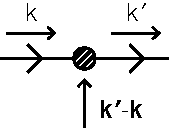
\includegraphics[scale=1]{resources/chap_ferm/fdiagapp_9.pdf}}\\
	&=&\adjustbox{raise=-6.1ex}{\includegraphics[scale=1]{resources/chap_ferm/fdiagapp_10.pdf}}+\adjustbox{raise=-6.1ex}{\includegraphics[scale=1]{resources/chap_ferm/fdiagapp_11.pdf}}+\cdots
\end{eqnarray} 

We have
\begin{equation}
	\adjustbox{raise=-6.1ex}{\includegraphics[scale=1]{resources/chap_ferm/fdiagapp_9.pdf}}=\adjustbox{raise=-6.1ex}{\includegraphics[scale=1]{resources/chap_ferm/fdiagapp_10.pdf}}+\adjustbox{raise=-6.1ex}{\includegraphics[scale=1]{resources/chap_ferm/fdiagapp_12.pdf}}
\end{equation}

Then
\begin{equation}
	t({\bf k},{\bf k'},\omega)=U({\bf k'}-{\bf k})+\int\frac{d^3{\bf k''}}{(2\pi)^3}U({\bf k''}-{\bf k})G({\bf k''},\omega)t({\bf k''},{\bf k'},\omega)
\end{equation}

In the case of delta-potential, we have
\begin{equation}
	U({\bf k'}-{\bf k})=U
\end{equation}

Then it's easy to see that $t({\bf k},{\bf k'},\omega)$ doesn't depend on ${\bf k},{\bf k'}$.

So
\begin{equation}
	t(\omega)=U+U\int\frac{d^3{\bf k''}}{(2\pi)^d}G({\bf k''},\omega)t(\omega)   
\end{equation}
and
\begin{equation}
	\int\frac{d^3{\bf k''}}{(2\pi)^d}G({\bf k''},\omega)=\int_{-\mu}^{\Lambda}d\epsilon N(\epsilon)\frac 1{\omega-\epsilon+i\delta{\rm sgn}\epsilon}
\end{equation}

Let's discuss the 2 dimensional case, $N(\epsilon)=N_0=\pi k_F^2/\mu$. Then
\begin{equation}
	\int_{-\mu}^{\Lambda}d\epsilon N(\epsilon)\frac 1{\omega-\epsilon+i\delta{\rm sgn}\epsilon}=-N_0\ln\Big[\frac{\omega-\Lambda}{\omega+\Lambda}\Big]\simeq-N_0\ln\Big[\frac{-\Lambda}{\omega+\Lambda}\Big]
\end{equation}

Then
\begin{equation}
	t(\omega)=\frac{U}{1+UN_0\ln\big[\frac{\Lambda}{-(\omega+\Lambda)}\big]}
\end{equation}

If $U<0$, $t(\omega)$ has a pole at $-\mu-\Lambda e^{-\frac 1{|U|N_0}}$. This is an example of the bound state. 

\section{Self Energy}

Let's consider a translational invariant system. The energy and momentum is conserved. In this system let's consider a particle $a$. 

A 1 particle irreducible(1PI) diagram for $a$ is defined as a connected diagram with exactly an incoming and an outgoing $a$ indices, and can not be broken into two connected diagrams by a cut on each $a-\bar a$ bond.

We define the self energy $\Sigma$ of $a$ as the sum of all different 1PIs:
\begin{equation}
	-i\Sigma(x_2-x_1)=\adjustbox{raise=-1.1ex}{\includegraphics[scale=1]{resources/chap_ferm/fdiagapp_13.pdf}}=\sum_{1PI}\adjustbox{raise=-1.1ex}{\includegraphics[scale=1]{resources/chap_ferm/fdiagapp_14.pdf}}
\end{equation}

Then the propogator of $a$ can be expressed as
\begin{eqnarray}
	\adjustbox{raise=-0.85ex}{\includegraphics[scale=1]{resources/chap_ferm/fdiagapp_15.pdf}}&=&\adjustbox{raise=-0.85ex}{\includegraphics[scale=1]{resources/chap_ferm/fdiagapp_16.pdf}}+\adjustbox{raise=-1.2ex}{\includegraphics[scale=1]{resources/chap_ferm/fdiagapp_17.pdf}}+\nonumber\\
	&&\adjustbox{raise=-1.2ex}{\includegraphics[scale=1]{resources/chap_ferm/fdiagapp_18.pdf}}+\cdots
\end{eqnarray}
You may check that we have the correct symmetric factor.

So we have the Dyson's equation
\begin{equation}
	\adjustbox{raise=-0.85ex}{\includegraphics[scale=1]{resources/chap_ferm/fdiagapp_15.pdf}}=\adjustbox{raise=-0.85ex}{\includegraphics[scale=1]{resources/chap_ferm/fdiagapp_16.pdf}}+\adjustbox{raise=-1.2ex}{\includegraphics[scale=1]{resources/chap_ferm/fdiagapp_19.pdf}}
\end{equation}

Let's view $G$,$G^0$ and $\Sigma$ as operators, then
\begin{equation}
	iG=iG_0+iG_0\cdot(-i)\Sigma\cdot iG_0
\end{equation}

So
\begin{equation}
	G=\frac 1{G_0^{-1}-\Sigma}
\end{equation}

If the system is translational invariant, then $\Sigma(p,p')=\Sigma(p)I_{p,p'}$. So
\begin{equation}
	G(p)=\frac 1{G_0^{-1}(p)-\Sigma(p) }
\end{equation}

Normally $G_0^{-1}(p)$ is real with an infinitesimal imaginary part, and $\Sigma(p)$ is small. For electron Green's function, let's break $\Sigma(p)$ into its real and imaginary part. Then
\begin{equation}
	G(p)=\frac 1{\omega -\tilde e_{\bf p}-\Re[\Sigma(p)]-i\Im[\Sigma(p)]}
\end{equation}

This has a pole $\omega_0=(\xi_p,\Im[\Sigma({\bf p},\omega_0)])=(\tilde e_{\bf p}+\Re[\Sigma({\bf p},\omega_0)],\Im[\Sigma({\bf p},\omega_0)])$. The real-time Green's function is
\begin{equation}
	G(t,{\rm p})=\int\frac{d\omega}{2\pi}e^{-i\omega}G(p)\sim\theta(t\omega_0)e^{-i\xi_p t}e^{-|Z_{\bf p}\Im[\Sigma({\bf p},\omega_0)]|t}
\end{equation}
where $Z_{\bf p}$ is the residue at the pole

So $\Im[\Sigma({\bf p},\omega_0)]$ determines the decay rate of the field $\psi_p$. The life time is $1/|Z_{\bf p}\Im[\Sigma({\bf p},\omega_0)]|$. Besides, $\tilde e_{\bf p}+\xi_p$ is the renormalized energy.
\section{Magnetic Susceptibility of Free Electron System}

The free electron system interact with external magnetic field by the Hamiltonian
\begin{equation}
	-\int \mu_B S(x)\cdot B(x,t)
\end{equation}
where
\begin{equation}
	S^i(x)=c^\dagger_\alpha\sigma_{\alpha\beta}^ic_\beta
\end{equation}

Then
\begin{equation}
	-i\chi^T_{ij}(x-x',t-t')=\mu_B^2\ \adjustbox{valign=c}{\includegraphics[scale=1]{resources/chap_ferm/fdiagapp_21.pdf}}
\end{equation}

Then
\begin{eqnarray}
	\chi^T_{ij}(q)(2\pi)^4\delta(q+q')&=&i\mu_B^2\ \adjustbox{valign=c}{\includegraphics[scale=1]{resources/chap_ferm/fdiagapp_22.pdf}}\\
	&=&i\mu_B^2\int dpdp'e^{i\delta p_0+i\delta p'_0}Tr[\sigma^j\sigma^i](-1)iG(p)iG(p')\delta(p-q-p')\nonumber\\
	&&\delta(p+q'-p')\\
	\chi^T_{ij}(q)&=&i\mu_B^22\delta_{ij}\int dpe^{2i\delta p_0-i\delta q_0}G(p)G(p-q)\\
	&=&i\mu_B^22\delta_{ij}\int\frac{dp}{(2\pi)^4}e^{2i\delta p_0-i\delta q_0}\frac 1{p_0-\epsilon_{\bf p}+i\delta {\rm sgn}\epsilon_{\bf p}}\frac 1{p_0-q_0+\epsilon_{{\bf p}-{\bf q}}+i\delta {\rm sgn}\epsilon_{{\bf p}-{\bf q}}}\\
	&=&\mu_B^22\delta_{ij}\int\frac{d{\bf p}}{(2\pi)^3}\frac {f_{{\bf p}-{\bf q}}-f_{\bf p}}{q_0-(\epsilon_{{\bf p}-{\bf q}}-\epsilon_{\bf p})+i\delta {\rm sgn}(\epsilon_{{\bf p}-{\bf q}}-\epsilon_{\bf p})}
\end{eqnarray}

Then
\begin{eqnarray}
	\chi_{ij}(q)&=&2\delta_{ij}\mu_B^2\int\frac{d{\bf p}}{(2\pi)^3}\frac {f_{{\bf p}-{\bf q}}-f_{\bf p}}{q_0-(\epsilon_{{\bf p}-{\bf q}}-\epsilon_{\bf p})+i\delta}\\
	&=&2\delta_{ij}\mu_B^2\Big[P\int\frac{d{\bf p}}{(2\pi)^3}\frac {f_{{\bf p}-{\bf q}}-f_{\bf p}}{q_0-(\epsilon_{{\bf p}-{\bf q}}-\epsilon_{\bf p})}-i\int\frac{d{\bf p}}{(2\pi)^3}(f_{{\bf p}-{\bf q}}-f_{\bf p})\delta(q_0-(\epsilon_{{\bf p}-{\bf q}}-\epsilon_{\bf p}))\Big]
\end{eqnarray}

\section{Jellium Model}

\part{Relativistic World}

\chapter{Classical Field Theory}

	A \index{classical field} classical field is a smooth map $\phi:M\rightarrow F$ from the base manifold $M$, which is usually 3+1D space-time, to some fiber space $F$. Intuitively, as illustrated in Fig \ref{fig:field}, there's a field quantity at every space-time point. Common fibre spaces includes $\mathbb{R}$, $\mathbb{C}$, $\mathbb{R}^N$, $\mathbb{C}^N$, spinor... 
	
	\begin{figure}[htb]
		\centering  
		\includegraphics[width=300pt]{resources/chap_classical/1_0_field.pdf}
		\caption{Classical field}
		\label{fig:field} 
	\end{figure}
	
	A field $\phi(x)=\phi(\vec x,t)=\phi_t(\vec x)$ can be regarded as a function of space, with $t$ as a parameter. As $t$ increases, the deformation of $\phi_t(\vec x)$ is called the evolution of the field. Here we study fields whose evolution are determined by the law of mechanics. Such fields must satisfy a set of equations. This is called the \index{EOM} equation of motion(EOM). A field that satisfies the EOM is said to be \index{on-shell field} on-shell (abbreviated for "on the mass shell", meaning that after Fourier transformation, the non-vanishing term $\phi_k$  satisfies $k^2=-m^2$), while a field that may not satisfy the EOM is said to be \index{off-shell field} off-shell. 
	
	\section{Lagrangian Formalism}
	In a dynamical system of classical field $\phi$ that has $n$ components, there exist a real scaler field $\mathcal{L}[\phi,\partial_\mu\phi,x^\mu]$ called \index{Lagrangian density} Lagrangian density. Lagrangian density is a functional of the $\phi$ and its first derivatives, and may also depend on $x^\mu$ explicitly. The form of Lagrangian density is decided by the nature of the dynamic system, and is considered known here. We define the \index{action} action $S$ in region $\Omega$ by the integral of the Lagrangian density:
	\begin{equation}
		S_\Omega=\int_{\Omega}d^4x\mathcal{L}[\phi,\partial_\mu\phi,x^\mu] \label{eqn:action}
	\end{equation}
	
	The core idea of the theory of classical fields is that: 
	
	An field with fixed value at  $\partial\Omega$ (the boundary of $\Omega$) is on-shell if and only if it satisfies the \index{Hamilton's principle} Hamilton's principle: the variation of the action in $\Omega$ according to the variation of the field is 0. 
	
	In other words, the action in $\Omega$ is stationary at on-shell fields. This leads to:
	\begin{eqnarray}
		\delta S_\Omega&=&\int_{\Omega}d^4x\delta\mathcal{L}[\phi,\partial_\mu\phi,x^\mu] \\
		&=&\int_{\Omega}d^4x\Big[\frac{\partial\mathcal{L}}{\partial\phi_i}\delta\phi_i+\frac{\partial\mathcal{L}}{\partial(\partial_\mu\phi_i)}\delta(\partial_\mu\phi_i)\Big]\\
		&=&\int_{\Omega}d^4x\Big[\frac{\partial\mathcal{L}}{\partial\phi_i}\delta\phi_i+\frac{\partial\mathcal{L}}{\partial(\partial_\mu\phi_i)}\partial_\mu(\delta\phi_i)\Big]\\
		&=&\int_{\Omega}d^4x\Big[\frac{\partial\mathcal{L}}{\partial\phi_i}\delta\phi_i+\partial_\mu\Big(\frac{\partial\mathcal{L}}{\partial(\partial_\mu\phi_i)}\delta\phi_i\Big)-\Big(\partial_\mu\frac{\partial\mathcal{L}}{\partial(\partial_\mu\phi_i)}\Big)\delta\phi_i\Big]	\\	&=&\int_{\Omega}d^4x\Big[\frac{\partial\mathcal{L}}{\partial\phi_i}-\partial_\mu\frac{\partial\mathcal{L}}{\partial(\partial_\mu\phi_i)}\Big]\delta\phi_i+\int_{\partial\Omega}dS_\mu\frac{\partial\mathcal{L}}{\partial(\partial_\mu\phi_i)}\delta\phi_i\\
		&=&\int_{\Omega}d^4x\Big[\frac{\partial\mathcal{L}}{\partial\phi_i}-\partial_\mu\frac{\partial\mathcal{L}}{\partial(\partial_\mu\phi_i)}\Big]\delta\phi_i \label{eqn:action-el}\\
		&=&0
	\end{eqnarray}
	
	Note that variation commutes with derivative because $\delta\partial_\mu\phi_i=\partial_\mu\phi'_i-\partial_\mu\phi_i=\partial_\mu(\phi'_i-\phi_i)=\partial_\mu\delta\phi_i$, and that $\delta \phi_i$ vanishes at $\partial\Omega$.
	
	Since $\delta\phi_i$ is arbitrary (as long as it's small), the condition
	\begin{equation}
		\int_{\Omega}d^4x\Big[\frac{\partial\mathcal{L}}{\partial\phi_i}-\partial_\mu\frac{\partial\mathcal{L}}{\partial(\partial_\mu\phi_i)}\Big]\delta\phi_i=0
	\end{equation}
	is equivalent to
	\begin{equation}
		\frac{\partial\mathcal{L}}{\partial\phi_i}=\partial_\mu\frac{\partial\mathcal{L}}{\partial(\partial_\mu\phi_i)}\label{eqn:E-L}
	\end{equation}
	in $\Omega$.
	
	This is called the \index{Euler-Lagrange equation}Euler-Lagrange equation. It is just the EOM in the theory of classical fields. According to theory of partial differential equation, there is always a solution with given boundary condition ($\phi_i(x)$ at $\partial\Omega$).
	
	\section{Hamiltonian Formalism}
	
	For the moment lets forget $\dot\phi_i=\frac{\partial\phi_i}{\partial t}$ and treat $\phi_i$ and $\dot\phi_i$ in $\mathcal{L}[\phi,\partial_\mu\phi,x^\mu]$ as independent degrees of freedom. 
	
	We define the \index{canonical momentum}canonical momentum as
	\begin{equation}
		\pi_i(x)=\frac{\partial\mathcal{L}}{\partial\dot\phi_i(x)}=\pi_i[\phi,\partial_\alpha\phi,\dot\phi,x^\mu] \label{eqn:canonical-momentum}
	\end{equation}
	where $\partial_\alpha$ is the spatial partial differentiation.
	
	Thus we can express $\dot\phi_i$ as a functional of $\phi$, $\partial_\alpha\phi$, $\pi$ and $x^\mu$. In Hamiltonian formalism, we use $\phi_i$ and $\pi_i$ as independent degrees of freedom.
	
	First we define the \index{Hamiltonian density}Hamiltonian density as the \index{Legendre transformation}Legendre transformation of $\mathcal{L}$
	\begin{equation}
		\mathcal{H}[\phi,\partial_\alpha\phi,\pi,x^\mu]=\big[\pi_i\dot\phi_i -\mathcal{L}[\phi,\partial_\alpha\phi,\dot\phi,x^\mu]\big]\big|_{\dot\phi=\dot\phi[\phi,\partial_\alpha\phi,\pi,x^\mu]}
	\end{equation}
	
	We have following relations
	\begin{eqnarray}
		\frac{\partial\mathcal{H}}{\partial\phi_i}&=&\pi_j\frac{\partial\dot\phi_j}{\partial\phi_i}-\frac{\partial\mathcal{L}}{\partial\phi_i}-\frac{\partial\mathcal{L}}{\partial\phi_{j,t}}\frac{\partial\dot\phi_j}{\partial\phi_i}=-\frac{\partial\mathcal{L}}{\partial\phi_i}\\
		\frac{\partial\mathcal{H}}{\partial\pi_i}&=&\dot\phi_i+\pi_j\frac{\partial\dot\phi_j}{\partial\pi_i}-\frac{\partial\mathcal{L}}{\partial\dot\phi_j}\frac{\partial\dot\phi_j}{\partial\pi_i}=\dot\phi_i\\
		\frac{\partial\mathcal{H}}{\partial(\partial_\alpha\phi_i)}&=&\pi_j\frac{\partial\dot\phi_j}{\partial(\partial_\alpha\phi_i)}-\frac{\partial\mathcal{L}}{\partial(\partial_\alpha\phi_i)}-\frac{\partial\mathcal{L}}{\partial\dot\phi_j}\frac{\partial\dot\phi_j}{\partial(\partial_\alpha\phi_i)}=-\frac{\partial\mathcal{L}}{\partial(\partial_\alpha\phi_i)}
	\end{eqnarray}
	
	Up to now, we have not determined the on-shell condition of $\pi$. However, we may impose one
	\begin{equation}
		\dot\phi_i=\partial_t\phi_i\Leftrightarrow \pi_i=\frac{\partial\mathcal{L}}{\partial\dot\phi_i(x)}\Bigg|_{\dot\phi_i=\partial_t\phi_i}
	\end{equation}
	
	The Euler-Lagrange equation can be reformulated into
	\begin{eqnarray}
		\frac{\partial\mathcal{L}}{\partial\phi_i}&=&\partial_\alpha\frac{\partial\mathcal L[\phi,\partial_\alpha\phi,\dot\phi,x^\mu]}{\partial(\partial_\alpha\phi_i)}+\partial_t\frac{\partial\mathcal L[\phi,\partial_\alpha\phi,\dot\phi,x^\mu]}{\partial(\dot\phi_i)}\\
		\dot\phi_i&=&\partial_t\phi_i
	\end{eqnarray}
	
	Use $\phi$ and $\pi$ as independent variables, we have the \index{Hamilton's equations}Hamilton's equations
	\begin{eqnarray}
		\partial_t\phi_i&=&\frac{\partial\mathcal{H}}{\partial\pi_i}\\
		\partial_t\pi_i&=&-\frac{\partial\mathcal{H}}{\partial\phi_i}+\partial_i\frac{\partial\mathcal{H}}{\partial(\partial_i\phi_i)}
	\end{eqnarray}
	
	\subsection{Generalized Hamilton's Principle}

	We can derive the Hamilton's equations from variational principle. We define a generalized Lagrangian density $\mathcal{L}'[\phi,\partial_\alpha\phi,\pi,x]$ as
	\begin{equation}
		\mathcal{L}'[\phi,\partial_\alpha\phi,\pi,x^\mu]=\pi_i\partial_t\phi_i-\mathcal{H}[\phi,\partial_i\phi,\pi,x^\mu]=\pi_i(\partial_t\phi_i-\dot\phi_i)+\mathcal{L}[\phi,\partial_\alpha\phi,\dot\phi,x^\mu] \label{eqn:general-l}
	\end{equation}
	where the independent fields are $\phi$ and $\pi$. We show that:	
	\begin{lemma}
		The on-shell $\phi$ and $\pi$ is the stationary path for the action
		\begin{equation}
			S'_\Omega=\int_{\Omega}d^4x\mathcal{L}'[\phi,\partial_\alpha\phi,\pi,x] \label{eqn:general-s}
		\end{equation}
	\end{lemma}
	\begin{proof}
	We require $S'_\Omega$ to be stationary while varying $\pi_i$, and get (note that we do not require $\delta\pi=0$ at $\partial\Omega$)	
	\begin{equation}
		\frac{\delta S'_\Omega}{\delta \pi_i}=\frac{\partial \mathcal{L}'}{\partial \pi_i}=\partial_t\phi_i-\dot\phi_i=0 \label{eqn:vary-pi}
	\end{equation}
	This is our new on-shell condition for $\pi$.
	
	Take (\ref{eqn:vary-pi}) into (\ref{eqn:general-l}), we get our good old Lagrange density again:	
	\begin{equation}
		\mathcal{L}'[\phi,\partial_\alpha\phi,\pi,x^\mu]\big|_{\dot\phi=\partial_t\phi}=\mathcal{L}[\phi,\partial_\mu\phi,x^\mu] \label{eqn:inv-legendre}
	\end{equation}
	This procedure is sometimes called the inverse of the Legendre transformation. Take (\ref{eqn:inv-legendre}) to (\ref{eqn:general-s}) and we get 	
	\begin{equation}
		S'_\Omega\big|_{\dot\phi=\partial_t\phi}=S_\Omega
	\end{equation}	
	
	We further require $S'_\Omega$ to be stationary while varying $\phi$. Obviously we get the Euler-Lagrange equation again.
	\end{proof}
	
	
	Since $\phi$ and $\pi$ are independent variables of the functional $S'_\Omega$, we may get the EOM by the so-called \index{generalized Hamilton's principle}generalized Hamilton's principle	
	\begin{equation}
		\delta S'_\Omega=0
	\end{equation}
	where variation is taken on $\pi(x)$ and $\phi(x)$.
	
	This leads the the \index{Hamilton's equations}Hamilton's equations	again
	\begin{eqnarray}
		\partial_t\phi_i&=&\dot\phi_i=\frac{\partial\mathcal{H}}{\partial\pi_i}\\
		\partial_t\pi_i&=&-\frac{\partial\mathcal{H}}{\partial\phi_i}+\partial_i\frac{\partial\mathcal{H}}{\partial(\partial_i\phi_i)}
	\end{eqnarray}
	
	\subsection{Dynamical Quantity}
	
	We can define the \index{Hamiltonian}Hamiltonian from the Hamiltonian density
	
	\begin{equation}
		H(t)=\int d^3x\mathcal{H}(x)
	\end{equation}
	
	Using (\ref{eqn:fun-deri}), we have the following relations	
	\begin{eqnarray}
		\frac{\delta H}{\delta\pi_i(x)}&=&\frac{\partial\mathcal{H}}{\partial\pi_i}(x)\\
		\frac{\delta H}{\delta\phi_i(x)}&=&\Big[\frac{\partial\mathcal{H}}{\partial\phi_i}-\partial_i\frac{\partial\mathcal{H}}{\partial(\partial_i\phi_i)}\Big](x)
	\end{eqnarray}
	
	Thus the Hamilton's equations can be re-expressed as 	
	\begin{eqnarray}
		\partial_t\phi_i(x)&=&\frac{\delta H}{\delta\pi_i(x)}\\
		\partial_t\pi_i(x)&=&-\frac{\delta H}{\delta\phi_i(x)}
	\end{eqnarray}
	
	A \index{dynamical quantity }dynamical quantity $Q(t)$ is the integral over space of some local functional $\mathcal{Q}[\phi,\partial_i\phi,\pi,\partial_i\pi,x^\mu]$
	\begin{equation}
		Q(t)=\int d^3x\mathcal{Q}(x)
	\end{equation}
	
	Clearly Hamiltonian is a dynamical quantity.
	
	\subsection{Poisson Bracket}
	
	Let $A$ and $B$ be two dynamical quantity, their \index{Poisson bracket}Poisson bracket is defined as	
	\begin{equation}
		\{A(t),B(t)\}=\int d^3x\Big[\frac{\delta A}{\delta \phi_i(x)}\frac{\delta B}{\delta \pi_i(x)}-\frac{\delta A}{\delta \pi_i(x)}\frac{\delta B}{\delta \phi_i(x)}\Big]
	\end{equation}
	It is also a dynamical quantity
	
	As in classical mechanics, Poisson bracket of dynamical quantities forms a Lie algebra called Poisson algebra.
	
	It's easy to check the following identity
	
	\begin{equation}
		\{\phi_i(\vec x,t),\pi_j(\vec y,t)\}=\delta^{(3)}(\vec x-\vec y)\delta_{ij}
	\end{equation}
	
	For on-shell field, the evolution of a dynamical quantity $Q$ is totally determined. It's EOM is
	\begin{eqnarray}
		\frac{dQ}{dt} &=&\lim_{\delta t\rightarrow 0}\frac 1 {\delta t}\bigg[\int d^3x\mathcal{Q}[\phi'(x),\partial_i\phi'(x),\pi'(x),\partial_i\pi'(x),x'^\mu]-\int d^3x\mathcal{Q}[\phi(x'),\partial_i\phi(x'), \nonumber\\
		&&\pi(x'),\partial_i\pi(x'),x^\mu]\bigg]+\lim_{\delta t\rightarrow 0}\frac 1 {\delta t}\bigg[\int d^3x\mathcal{Q}[\phi'(x),\partial_i\phi'(x),\pi'(x),\partial_i\pi'(x),x^\mu]\nonumber\\
		&&-\int d^3x\mathcal{Q}[\phi(x),\partial_i\phi(x),\pi(x),\partial_i\pi(x),x^\mu]\bigg]\\
		&=&\int d^3x\frac{\partial \mathcal{Q}}{\partial t}+\lim_{\delta t\rightarrow 0}\frac 1 {\delta t}\int d^3x\Big[\frac{\delta \mathcal{Q}}{\delta \phi_i(x)}(\phi'_i(x)-\phi_i(x))+\frac{\delta \mathcal{Q}}{\delta \pi_i(x)}(\pi'_i(x)-\pi_i(x))\Big] \\
		&=&\frac{\partial Q}{\partial t}+\int d^3x\Big[\frac{\delta \mathcal{Q}}{\delta \phi_i(x)}\partial_t\phi_i(x)+\frac{\delta \mathcal{Q}}{\delta \pi_i(x)}\partial_t\pi_i(x)\Big] \\
		&=&\frac{\partial Q}{\partial t}+\int d^3x\Big[\frac{\delta \mathcal{Q}}{\delta \phi_i(x)}\frac{\delta H}{\delta\pi_i(x)}-\frac{\delta \mathcal{Q}}{\delta \pi_i(x)}\frac{\delta H}{\delta\phi_i(x)}\Big] \\
		&=&\frac{\partial Q}{\partial t}+\{Q,H\}
	\end{eqnarray}
	where $x'^\mu=x^\mu+\delta t\delta^\mu_0$, $\phi_i'(x)=\phi_i(x')$ and $\pi_i'(x)=\pi_i(x')$. During the derivation we have used (\ref{eqn:vari-int}) and the Hamilton's equations.
	\section{Symmetry}
	A \index{symmetry operation}symmetry operation $(T,P)$ is a diffeomorphism $T$ of the base manifold together with an invertible field transformation $P$ such that for any subregion $\omega$ of the base manifold $\Omega$, we have
	\begin{equation}
		\int_{\omega}d^4x\mathcal{L}[\phi,\partial_\mu\phi,x^\mu]=\int_{\omega'}d^4x\mathcal{L}[\phi',\partial_\mu\phi',x^\mu]
	\end{equation}
	where $\omega'=T\omega$ and $\phi'=P(T\phi)$, and $T$ acts on $\phi$ by $(T\phi)(x)=\phi(T^{-1}x)$. From Hamilton's principle, it's clear that if $\phi$ is on-shell on $\omega$, $\phi'$ is also on-shell on $\omega'$ with boundary condition $\phi'$ at $\partial\omega'$.


	If $T\neq id$, the symmetry operation is called \index{space-time symmetry}space-time symmetry. Otherwise it is called \index{internal symmetry}internal symmetry.
	
	We impose two symmetry operations $(T,P)$ and $(T',P')$ successively:
	
	\begin{equation}
	\int_{\omega}d^4x\mathcal{L}[\phi,\partial_\mu\phi,x^\mu]=\int_{\omega'}d^4x\mathcal{L}[\phi',\partial_\mu\phi',x^\mu]=\int_{\omega''}d^4x\mathcal{L}[\phi'',\partial_\mu\phi'',x^\mu]
	\end{equation}
	where
	\begin{eqnarray}
		\omega''&=&T'\omega'=(T'\circ T)\omega\\
		\phi''&=&(P'\circ T')\phi'=(P'\circ T'\circ P\circ T)\phi=(P'\circ T'\circ P\circ T'^{-1})((T'\circ T)\phi)
	\end{eqnarray}
	
	 This shows that $(T'\circ T,P'\circ T'\circ P\circ                                                                                                                                  T'^{-1})$ is also a symmetry operation. So symmetry operations form a monoid under composition
	\begin{equation}
		(T',P')\circ(T,P)=(T'\circ T,P'\circ T'\circ P\circ T'^{-1})
	\end{equation}
	while the unit element is $(id,id)$. It's easy to see that $(T,P)^{-1}=(T^{-1},T^{-1}P^{-1}T)$, so symmetry operations form a group. This is called the \index{symmetry group}symmetry group of a dynamical system. A dynamical system is called to have discreet/continuous symmetry if its symmetry group is a discreet/Lie group.
	
	\paragraph{Example}We define the symmetry operation $(T_\theta,P_\theta)$ on a vector field $A^\mu(x)$ parameterized by $\theta$ as	
	\begin{equation}
		T_\theta\begin{pmatrix}
		x^0 \\
		x^1\\
		x^2 \\
		x^3
		\end{pmatrix} 
		 =
		\begin{pmatrix}
		0 &0 & 0& 0\\
		0& \cos\theta &-\sin\theta &0 \\
		0&\sin\theta & \cos\theta &0 \\
		0& 0& 0& 0
		\end{pmatrix} 
		\begin{pmatrix}
		x^0 \\
		x^1\\
		x^2 \\
		x^3
		\end{pmatrix} 
	\end{equation}	
	\begin{equation}
		P_\theta \begin{pmatrix}
		A^0 \\
		A^1\\
		A^2 \\
		A^3
		\end{pmatrix} 
		=
		\begin{pmatrix}
		0 &0 & 0& 0\\
		0& \cos\theta &-\sin\theta &0 \\
		0&\sin\theta & \cos\theta &0 \\
		0& 0& 0& 0
		\end{pmatrix} 
		\begin{pmatrix}
		A^0 \\
		A^1\\
		A^2 \\
		A^3
		\end{pmatrix} 
	\end{equation}	

	\begin{figure}[htb]
		\centering  
		\includegraphics[width=200pt]{resources/chap_classical/1_4_symmetry.pdf}
		\caption{Continous symmetry operation}
		\label{fig:symmetry} 
	\end{figure}
	
	As illustrated in Fig \ref{fig:symmetry}, this is a continuous symmetry, and is the subgroup of the symmetry group of the system with Lagrangian density	
	\begin{equation}
		\mathcal{L}=(\partial^\mu A^\nu-\partial^\nu A^\mu)(\partial_\mu A_\nu-\partial_\nu A_\mu)+\alpha A^\mu A_\mu
	\end{equation}	
	
	\paragraph{Example} Consider a Lagrangian density of a scalar field $\phi$
	\begin{equation}
		\mathcal{L}=\phi^2+\partial^\mu \phi \partial_\mu\phi+ \sum_{\mu}e^{-(x^\mu)^2}
	\end{equation}	
	
	Its symmetry group is a discreet group mapping axes to axes. 
	\subsection{Noether's Theorem}
	
	\index{Noether's theorem}Noether's theorem states that if a system has a continuous symmetry $G$, then each one-parameter subgroup of $G$ corresponds to a \index{conserved current}conserved current $j^\mu[\phi,\partial_\mu\phi,x^\mu]$ such that $\partial_\mu j^\mu=0$ when $\phi$ is on-shell.
	
	Suppose the one-parameter subgroup is $(T_\epsilon,P_\epsilon)$ parameterized by $\epsilon$, with Lie algebra $(\mathcal T,\mathcal P)$. The infinitesimal symmetry operation is
	\begin{equation}
		(T_\epsilon,P_\epsilon)=(id+\epsilon\mathcal T,id+\epsilon\mathcal P)
	\end{equation}
	which act on $x$ and $\phi$ as
	\begin{eqnarray}
		x&\longrightarrow&x'=T_\epsilon x=x+\epsilon\mathcal Tx=x+\delta x\\
		\phi(x)&\longrightarrow&\phi'(x)=P_\epsilon\phi(T_\epsilon^{-1}x)=\phi(x-\epsilon\mathcal Tx)+\epsilon\mathcal P\phi(x)=\phi(x)+\delta\phi(x)
	\end{eqnarray}
	
	Then
	\begin{eqnarray}
		\delta x^\mu&=&\epsilon(\mathcal Tx)^\mu \label{eqn:dx}\\
		\delta\phi_i(x)&=&\phi_i(x-\epsilon\mathcal Tx)-\phi_i(x)+\epsilon(\mathcal P\phi)_i(x)\\
		&=&-\epsilon\partial_\mu\phi_i(x)(\mathcal Tx)^\mu+\epsilon(\mathcal P\phi)_i(x) \label{eqn:dphi}
	\end{eqnarray}
	
	From the definition of symmetry, we have
	\begin{eqnarray}
		\int_{\omega}d^4x\mathcal{L}[\phi,\partial_\mu\phi,x^\mu]&=&\int_{\omega'}d^4x\mathcal{L}[\phi',\partial_\mu\phi',x^\mu]\\
		&=&\int_{\omega}d^4x\mathcal{L}[\phi',\partial_\mu\phi',x^\mu]+\int_{\partial\omega}dS_\mu\delta x^\mu\mathcal{L}[\phi',\partial_\mu\phi',x^\mu]\\
		&=&\int_{\omega}d^4x\Big[\mathcal{L}[\phi',\partial_\mu\phi',x^\mu]+\partial_\mu\big[\delta x^\mu\mathcal{L}[\phi',\partial_\mu\phi',x^\mu]\big]\Big]
	\end{eqnarray}
	
	So
	\begin{eqnarray}
		0&=&\int_{\omega}d^4x\Big[\mathcal{L}[\phi',\partial_\mu\phi',x^\mu]-\mathcal{L}[\phi,\partial_\mu\phi,x^\mu]+\partial_\mu\big[\delta x^\mu\mathcal{L}[\phi',\partial_\mu\phi',x^\mu]\big]\Big]\\
		&=&\int_{\omega}d^4x\Big[\frac{\partial\mathcal{L}}{\partial\phi_i}\delta\phi_i+\frac{\partial\mathcal{L}}{\partial(\partial_\mu\phi_i)}\partial_\mu\delta\phi_i+\partial_\mu(\delta x^\mu\mathcal{L})\Big]\\
		&=&\int_{\omega}d^4x\Big[\Big(\frac{\partial\mathcal{L}}{\partial\phi_i}-\partial_\mu\frac{\partial\mathcal{L}}{\partial(\partial_\mu\phi_i)}\Big)\delta\phi_i+\partial_\mu\Big(\frac{\partial\mathcal{L}}{\partial(\partial_\mu\phi_i)}\delta\phi_i+\delta x^\mu\mathcal{L}\Big)\Big]
	\end{eqnarray}
	
	Since $\omega$ is arbitrary, the integrand must be zero everywhere
	\begin{equation}
		\Big(\frac{\partial\mathcal{L}}{\partial\phi_i}-\partial_\mu\frac{\partial\mathcal{L}}{\partial(\partial_\mu\phi_i)}\Big)\delta\phi_i+\partial_\mu\Big(\frac{\partial\mathcal{L}}{\partial(\partial_\mu\phi_i)}\delta\phi_i+\delta x^\mu\mathcal{L}\Big)=0 \label{eqn:nother_a}
	\end{equation}
	
	We define the conserved current	as
	\begin{equation}
		j^\mu=\frac 1 \epsilon\Big(\frac{\partial\mathcal{L}}{\partial(\partial_\mu\phi_i)}\delta\phi_i+\delta x^\mu\mathcal{L}\Big) \label{eqn:current}
	\end{equation}
	
	It's easy to see when $\phi$ is on-shell, $\partial_\mu j^\mu=0$.
	
	We take (\ref{eqn:dx}) and (\ref{eqn:dphi}) into (\ref{eqn:current}), and get the final expression of the conserved current	
	\begin{eqnarray}
		j^\mu&=&\Big(\frac{\partial\mathcal{L}}{\partial(\partial_\mu\phi_i)}\partial_\nu\phi_i(\mathcal Tx)^\nu-(\mathcal T x)^\mu\mathcal{L}\Big)-\frac{\partial\mathcal{L}}{\partial(\partial_\mu\phi_i)}(\mathcal P\phi)_i\\
		&=&\Big(\frac{\partial\mathcal{L}}{\partial(\partial_\mu\phi_i)}\partial_\nu\phi_i-\mathcal{L}\delta^\mu_\nu\Big)(\mathcal Tx)^\nu-\frac{\partial\mathcal{L}}{\partial(\partial_\mu\phi_i)}(\mathcal P\phi)_i \label{eqn:current2}
	\end{eqnarray}
	
	We further define the \index{conserved charge}conserved charge $Q$ in region $\Omega$ as 	
	\begin{equation}
		Q_\Omega=\int_\Omega d^3xj^0
	\end{equation}
	
	When $\phi$ is on-shell, the time derivative of $Q_\Omega$ is
	\begin{eqnarray}
		\frac{dQ_\Omega}{dt}&=&\int_\Omega d^3x\partial_0j^0 \\
		&=&-\int_\Omega d^3x\partial_ij^i \\
		&=&-\int_{\partial\Omega} dS_ij^i 
	\end{eqnarray}
	
	This is often interpreted as the growth of the total charge inside a region is the same as the amount of charge that flows inside. This also describes the physics of incompressible flow.
	
	We say that two \index{equivalent conserved currents}conserved currents are \textbf{equivalent} if they give the same conserved charge up to a boundary term.
	
	With a conserved current $j$, we can construct a conserved current 
	\begin{equation}
	j'^\mu=j^\mu+\partial_\nu k^{\mu\nu}
	\end{equation}
	where $k^{\mu\nu}=-k^{\nu\mu}$.
	
	From
	\begin{equation}
	Q'_{\Omega}=\int_\Omega d^3x j'^0=\int_\Omega d^3x(j^0+\partial_\nu k^{0\nu})=Q_{1\Omega}+\int_{\partial\Omega} dS_\nu k^{0\nu}
	\end{equation}
	we see that $j$ and $j'$ are equivalent.
	
	\subsection{Change of Action by an Arbitrary Spatial Difference}
		
	For the future proof of Ward identity, we will study a slightly modified transformation:
	\begin{eqnarray}
		x&\longrightarrow&x'=T_\epsilon x=x+\epsilon(x)\mathcal Tx=x+\delta x\\
		\phi(x)&\longrightarrow&\phi'(x)=P_\epsilon\phi(T_\epsilon^{-1}x)=\phi(x-\epsilon(x)\mathcal Tx)+\epsilon(x)\mathcal P\phi(x)=\phi(x)+\delta\phi(x)
	\end{eqnarray}
	
	So
	\begin{eqnarray}
		\delta x^\mu&=&\epsilon(x)(\mathcal Tx)^\mu\\
		\delta\phi_i(x)&=&\phi_i(x-\epsilon(x)\mathcal Tx)-\phi_i(x)+\epsilon(x)(\mathcal P\phi)_i(x)\\
		&=&-\epsilon(x)\partial_\mu\phi_i(x)(\mathcal Tx)^\mu+\epsilon(x)(\mathcal P\phi)_i(x)
	\end{eqnarray}
	
	By the definition of symmetry, if $\epsilon(x)$ is a small const, $\delta S=0$. However if $\epsilon(x)$ is non-const,
	\begin{eqnarray}
		\delta S_\epsilon&=&\int_{\omega'}d^4x\mathcal{L}[\phi',\partial_\mu\phi',x^\mu]-\int_{\omega}d^4x\mathcal{L}[\phi,\partial_\mu\phi,x^\mu]\\
		&=&\int_{\omega}d^4x\Big[\Big(\frac{\partial\mathcal{L}}{\partial\phi_i}-\partial_\mu\frac{\partial\mathcal{L}}{\partial(\partial_\mu\phi_i)}\Big)\delta\phi_i+\partial_\mu\Big(\frac{\partial\mathcal{L}}{\partial(\partial_\mu\phi_i)}\delta\phi_i+\delta x^\mu\mathcal{L}\Big)\Big]\\
		&=&\int_{\omega}d^4x[A\epsilon(x)-j^\mu\partial_\mu\epsilon(x)]
	\end{eqnarray}
	where $A$ is just the LHS of (\ref{eqn:nother_a}) and is $0$ (even for off-shell field).
	
	So
	\begin{equation}
		\delta S_\epsilon=-\int_{\omega}d^4x j^\mu\partial_\mu\epsilon(x)
	\end{equation}
	
	Consider two equivalent currents $j^\mu$ and $j'^\mu$ such that
	\begin{equation}
	j'^\mu=j^\mu+\partial_\nu k^{\mu\nu}
	\end{equation}
	where $k^{\mu\nu}=-k^{\nu\mu}$.
	
	From
	\begin{eqnarray}
		&&-\int_{\omega}d^4x (j^\mu+\partial_\nu k^{\mu\nu})\partial_\mu\epsilon(x)\\
		&=&-\int_{\omega}d^4x j^\mu\partial_\mu\epsilon(x)-\int_{\omega}d^4x \partial_\nu k^{\mu\nu}\partial_\mu\epsilon(x)\\
		&=&-\int_{\omega}d^4x j^\mu\partial_\mu\epsilon(x)-\int_{\omega}d^4x\partial_\mu( \partial_\nu k^{\mu\nu}\epsilon(x))-\int_{\omega}d^4x\partial_\mu\partial_\nu k^{\mu\nu}\epsilon(x)\\
		&=&-\int_{\omega}d^4x j^\mu\partial_\mu\epsilon(x)-\int_{\partial\omega}dS_\mu\partial_\nu k^{\mu\nu}\epsilon(x)
	\end{eqnarray}
	we see that the two equivalent currents give the same $\delta S_\epsilon$ up to a boundary term.
	\subsection{Poincar\'e Symmetry}
	
	Poincar\'e group $P$ is the group isometry transformation of $\mathbb R^4$, whose element $T_{\Lambda,a}$ is parameterized by Lorentz transformation $\Lambda$ and translation $a^\mu$, and acts on $x^\mu$ as 
	\begin{equation}
		T_{\Lambda,a}x=\Lambda x+a
	\end{equation}	
	
	Due to the principle of special relativity, a relativistic field must have \index{Poincar\'e symmetry}Poincar\'e symmetry. Denote the symmetry group of the field as $S$. That is, relative to each neighborhood $N(T_{\Lambda,a})$ of $P$, there exists a smooth $S$-valued function $(T_{\Lambda',a'},P_{\Lambda',a'})$ as function of $T_{\Lambda',a'}\in N(T_{\Lambda,a})$.
	
	Here we make two asumptions:
	\begin{enumerate}
		\item $(T_{1,a},1)$ is a symmetry operation.
		\item $P$ commutes with $T$ when acting on fields. So $(T_{\Lambda,a},P_{\Lambda,a})(T_{\Lambda',a'},P_{\Lambda',a'})=(T_{\Lambda,a}T_{\Lambda',a'},P_{\Lambda,a}P_{\Lambda',a'})$
	\end{enumerate}
	
	If $(T_{\Lambda,a},P_{\Lambda,a})\in S$ then 
	\begin{equation}
		(T_{\Lambda,0},P_{\Lambda,a})=(T_{1,a},1)^{-1}(T_{\Lambda,a},P_{\Lambda,a}) \in S
	\end{equation}
	If furthermore $(T_{\Lambda,0},P_{\Lambda,0})\in S$ then  
	\begin{equation}
		(1,P_{\Lambda,0}P_{\Lambda,a}^{-1})=(T_{\Lambda,0},P_{\Lambda,0})(T_{\Lambda,0},P_{\Lambda,a})^{-1}\in S
	\end{equation}
	
	Define 
	\begin{equation}
		G=\{g|(1,g) {\rm \ is \ symmetry}\}
	\end{equation}
	Obviously $G$ is a group. And we have shown that 
	\begin{equation}
		(T_{\Lambda,a},P_{\Lambda,a})\in S\wedge(T_{\Lambda,0},P_{\Lambda,0})\in S \Rightarrow P_{\Lambda,0}P_{\Lambda,a}^{-1}\in G
	\end{equation}
	
	Then  
	\begin{equation}
		(T_{\Lambda,a},P_{\Lambda,a})\in S\wedge(T_{\Lambda,0},P_{\Lambda,0})\in S \Rightarrow(T_{\Lambda,a},P_{\Lambda,0})=(1,P_{\Lambda,0}P_{\Lambda,a}^{-1})(T_{\Lambda,a},P_{\Lambda,a})\in S
	\end{equation}
	
	Since there must be some $(T_{\Lambda,a},P_{\Lambda,a})\in S$, we have
	\begin{equation}
		(T_{\Lambda,0},P_{\Lambda,0})\in S \Rightarrow(T_{\Lambda,a},P_{\Lambda,0})\in S
	\end{equation}
	
	 That means, we may choose a smooth $S$-valued function $(T_{\Lambda',a'},P_{\Lambda',0})$ in each $(\Lambda',a')\in(N(\Lambda),\mathbb R^4)$ where $N(\Lambda)$ is a neighborhood of $\Lambda$, as long as $P_{\Lambda',0}$ is smooth in $N(\Lambda)$
	
	So there is a one-one correspondence between the possible piece-wise smooth $(T_{\Lambda,a},P_{\Lambda,a})$ and the possible piece-wise smooth $P_{\Lambda,0}$ together the possible $G$. So it's enough to just study the Lorentz symmetry $(T_\Lambda,P_\Lambda)=(T_{\Lambda,0},P_{\Lambda,0}).$ Clearly the possible piece-wise smooth $P_{\Lambda}=P_{\Lambda,0}$ is just the cover space of $L_+^\uparrow$. The only continuous cover space of $L_+^\uparrow$ is $L_+^\uparrow$ and $SL(2,\mathbb C)$.  Thus, the possible fields classified by Lorentz symmetry include:
	\begin{enumerate}
		\item Scalar field, vector field, tensor field ... whose Lorentz symmetry is $(T_\Lambda,P_\Lambda)$, where $P_\Lambda$ is isomorphic to $L_+^\uparrow$.
		\item Spinor field ... whose Lorentz symmetry is $(T_\Lambda,\pm P_\Lambda)$, where $\pm P_\Lambda$s is isomorphic to $SL(2,\mathbb C)$. The relationship between $\Lambda$ and $P_\Lambda$ is illustrated in Fig. \ref{fig:lorentz}.
		\begin{figure}[htb]
			\centering  
			\includegraphics[width=230pt]{resources/chap_classical/1_7_lorentz.pdf}
			\caption{The relationship between $\Lambda$ and $P_\Lambda$.}
			\label{fig:lorentz} 
		\end{figure}
	\end{enumerate} 

	
	\subsection{Conserved Current of Poincar\'e Symmetry}
	The infinitesimal transformation of translation is $(\epsilon^\alpha,id)$. Its Lie algebra is $(\delta^\alpha,0)$, where
	\begin{equation}
		(\delta^\alpha x)^\mu=\eta^{\alpha\mu}\\
	\end{equation}
	
	And the conserved currents are
	\begin{eqnarray}
		j^{\mu,\alpha}&=&\Big(\frac{\partial\mathcal{L}}{\partial(\partial_\mu\phi_i)}\partial_\nu\phi_i-\mathcal{L}\delta^\mu_\nu\Big)(\delta^\alpha x)^\nu\\
		&=&\frac{\partial\mathcal{L}}{\partial(\partial_\mu\phi_i)}\partial^\alpha\phi_i-\mathcal{L}\eta^{\mu\alpha}
	\end{eqnarray}
	
	We define the \index{energy-momentum tensor}energy-momentum tensor $T^{\mu\nu}$ as 
	\begin{equation}
		T^{\mu\nu}=j^{\mu,\nu}
	\end{equation}
	with conserved charges as
	\begin{eqnarray}
		P^\mu&=&\int d^3xT^{0\mu}\\
		&=&\int d^3x \frac{\partial\mathcal{L}}{\partial(\partial_0\phi_i)}\partial^\mu\phi_i-\mathcal{L}\eta^{0\mu}\\
		&=&\int d^3x \pi_i\partial^\mu\phi_i-\mathcal{L}\eta^{0\mu}
	\end{eqnarray}	
	which are called \index{momentum 4-vector} momentum 4-vector.
	
	It can be easily checked that the current of any symmetry can be expressed as
	\begin{equation}
		j^\mu=T^\mu_{\ \nu}(\mathcal Tx)^\nu-\frac{\partial\mathcal{L}}{\partial(\partial_\mu\phi_i)}(\mathcal P\phi)_i
	\end{equation}
	
	The term $\frac{\partial\mathcal{L}}{\partial(\partial_\mu\phi_i)}(\mathcal P\phi)_i$ is annoying and can be eliminated for space-time symmetry (in the case of equivalent conserved current) in some cases.
	
	The infinitesimal transformation of rotation(including boost) is $(\Lambda_\epsilon^{\alpha\beta},P_{\Lambda_\epsilon^{\alpha\beta}})$. Its Lie algebra is $(\mathcal M^{\alpha\beta},\mathcal P^{\alpha\beta})$, where
	\begin{equation}
		(\mathcal M^{\alpha\beta} x)^\mu=\eta^{\alpha\mu}x^\beta-\eta^{\beta\mu}x^\alpha
	\end{equation}
	
	And the conserved currents are
	\begin{eqnarray}
		j^{\mu,\alpha\beta}&=&\Big(\frac{\partial\mathcal{L}}{\partial(\partial_\mu\phi_i)}\partial_\nu\phi_i-\mathcal{L}\delta^\mu_\nu\Big)(\mathcal M^{\alpha\beta} x)^\nu-\frac{\partial\mathcal{L}}{\partial(\partial_\mu\phi_i)}(\mathcal P^{\alpha\beta}\phi)_i\\
		&=&\Big(\frac{\partial\mathcal{L}}{\partial(\partial_\mu\phi_i)}\partial_\nu\phi_i-\mathcal{L}\delta^\mu_\nu\Big)(\eta^{\alpha\nu}x^\beta-\eta^{\beta\nu}x^\alpha)-\frac{\partial\mathcal{L}}{\partial(\partial_\mu\phi_i)}(\mathcal P^{\alpha\beta}\phi)_i\\
		&=&(T^{\mu\alpha}x^\beta-T^{\mu\beta}x^\alpha)-\frac{\partial\mathcal{L}}{\partial(\partial_\mu\phi_i)}(\mathcal P^{\alpha\beta}\phi)_i \label{eqn:agu_momen}
	\end{eqnarray}
	which we may also call $J^{\mu\alpha\beta}$
	
	The conserved charge of $J^{\mu\alpha\beta}$ is 
	\begin{eqnarray}
		M^{\mu\nu}&=&\int d^3xj^{0,\mu\nu}
	\end{eqnarray}
	which are called \index{angular momentum tensor}angular momentum tensors.
	
	We define the Belinfante tensor as
	\begin{equation}
		B^{\mu\nu\rho}=\frac 12\Big[\frac{\partial\mathcal L}{\partial(\partial_\mu\phi_i)}(\mathcal P^{\nu\rho}\phi)_i+\frac{\partial\mathcal L}{\partial(\partial_\nu\phi_i)}(\mathcal P^{\rho\mu}\phi)_i-\frac{\partial\mathcal L}{\partial(\partial_\rho\phi_i)}(\mathcal P^{\mu\nu}\phi)_i\Big]
	\end{equation}
	
	We assume $\mathcal P^{\mu\nu}=-\mathcal P^{\nu\mu}$, which leads to $B^{\mu\nu\rho}=-B^{\nu\mu\rho}$. 
	
	We define the Belinfante energy-momentum tensor $T_B^{\mu\nu}$ as
	
	\begin{equation}
		T_B^{\mu\nu}=T^{\mu\nu}+\partial_\rho B^{\rho\mu\nu}
	\end{equation}
	
	Since $B^{\rho\mu\nu}$ is anti-symmetric in $\rho$ and $\mu$, $T_B^{\mu\nu}$ and $T^{\mu\nu}$ are equivalent.
	
	Applying $\partial_\mu$ to (\ref{eqn:agu_momen}), and we have
	\begin{equation}
		T^{\alpha\beta}-T^{\beta\alpha}=\partial_\mu\frac{\partial\mathcal{L}}{\partial(\partial_\mu\phi_i)}(\mathcal P^{\alpha\beta}\phi)_i
	\end{equation}
	
	So
	\begin{equation}
		T_B^{\mu\nu}-T_B^{\nu\mu}=0
	\end{equation},
	that is, $T_B^{\mu\nu}$ is symmetric.
	
	We may define
	\begin{equation}
		J_B^{\mu\nu\rho}=T_B^{\mu\nu}x^\rho-T_B^{\mu\rho}x^\nu
	\end{equation}
	
	We have
	\begin{eqnarray}
		J_B^{\mu\nu\rho}&=&T^{\mu\nu}x^\rho-T^{\mu\rho}x^\nu+(x^\rho\partial_\alpha B^{\alpha\mu\nu}-x^\nu\partial_\alpha B^{\alpha\mu\rho})\\
		&=&T^{\mu\nu}x^\rho-T^{\mu\rho}x^\nu+\partial_\alpha(x^\rho B^{\alpha\mu\nu}-x^\nu B^{\alpha\mu\rho})-(B^{\rho\mu\nu}- B^{\nu\mu\rho})\\
		&=&T^{\mu\nu}x^\rho-T^{\mu\rho}x^\nu-\frac{\partial\mathcal{L}}{\partial(\partial_\mu\phi_i)}(\mathcal P^{\alpha\beta}\phi)_i+\partial_\alpha(x^\rho B^{\alpha\mu\nu}-x^\nu B^{\alpha\mu\rho})\\
		&=&J^{\mu\nu\rho}+\partial_\alpha(x^\rho B^{\alpha\mu\nu}-x^\nu B^{\alpha\mu\rho})
	\end{eqnarray}
	
	Since $x^\rho B^{\alpha\mu\nu}-x^\nu B^{\alpha\mu\rho}$ is anti-symmetric in $\alpha$ and $\mu$, $J^{\mu\nu\rho}$ and $J_B^{\mu\nu\rho}$ are equivalent.
	
	\subsection{Scale Invariance and It's Currents}
	
	The scale transformation is $(T_\lambda,P_\lambda)$ that acts on $x$ and $\phi$ as
	\begin{eqnarray}
		T_\lambda x&=&\lambda x\\
		P_\lambda \phi&=&\lambda^{-\Delta}\phi
	\end{eqnarray}
	
	It's Lie algebra is $(1,-\Delta)$. And the conserved current is
	\begin{equation}
		j^\mu=T^\mu_{\ \nu}x^\nu+\Delta\frac{\partial\mathcal{L}}{\partial(\partial_\mu\phi_i)}\phi_i 
	\end{equation}
	which we may also call $D^\mu$.
	
	Define the virial of $\phi$ as
	\begin{equation}
		V^\mu=\frac{\partial \mathcal L}{\partial (\partial^\rho\phi_i)}(\eta^{\mu\rho}+\mathcal P^{\mu\rho})\phi_i
	\end{equation}
	
	Assume that 
	\begin{equation}
		V^\mu=\partial_\alpha\sigma^{\alpha\mu}
	\end{equation}
	and also assume the dimension of the space-time is $d>2$.
	
	Define
	\begin{eqnarray}
		\sigma_+^{\mu\nu}&=&\frac 12 (\sigma^{\mu\nu}+\sigma^{\nu\mu})\\
		X^{\lambda\rho\mu\nu}&=&\frac 2{d-2}\big\{\eta^{\lambda\rho}\sigma_+^{\mu\nu}-\eta^{\lambda\mu}\sigma_+^{\rho\nu}-\eta^{\lambda\nu}\sigma_+^{\rho\mu}+\eta^{\mu\nu}\sigma_+^{\lambda\rho}+\frac 1{d-1}(\eta^{\lambda\rho}\eta^{\mu\nu}-\eta^{\lambda\mu}\eta^{\rho\nu})\sigma^\alpha_{+\alpha}\big\}
	\end{eqnarray}
	
	We define
	\begin{equation}
		T_X^{\mu\nu}=T^{\mu\nu}+\partial_\rho B^{\rho\mu\nu}+\frac 12 \partial_\lambda\partial_\rho X^{\lambda\rho\mu\nu}
	\end{equation}
	
	It's easy to see that
	\begin{equation}
		\partial_\lambda\partial_\rho\partial_\mu X^{\lambda\rho\mu\nu}=0
	\end{equation}
	
	So $T_X^{\mu\nu}$ is a conserved current. It's easy to see that $T_X^{\mu\nu}$ and $T^{\mu\nu}$ are equivalent and give the same $\delta S_\epsilon$.
	
	Define
	\begin{equation}
		J_X^{\mu\nu\rho}=T_X^{\mu\nu}x^\rho-T_X
		^{\mu\rho}x^\nu
	\end{equation}
	It's easy to see that $J_X^{\mu\nu\rho}$ and $J^{\mu\nu\rho}$ are equivalent and give the same $\delta S_\epsilon$.
	
	Define
	\begin{equation}
		D_X^\mu=T^\mu_{X\nu}x^\nu
	\end{equation}
	
	We have
	\begin{eqnarray}
		D_X^\mu&=&T^\mu_{\ \nu}x^\nu+\partial_\rho B^{\rho\mu}_{\quad\nu}x^\nu+\frac 12 \partial_\lambda\partial_\rho X^{\lambda\rho\mu}_{\quad\ \nu}x^\nu\\
		&=&T^\mu_{\ \nu}x^\nu+\partial_\rho (B^{\rho\mu}_{\quad\nu}x^\nu)-B^{\rho\mu}_{\quad\rho}+\frac 12 \partial_\lambda\partial_\rho X^{\lambda\rho\mu}_{\quad\ \nu}x^\nu\\
		&=&T^\mu_{\ \nu}x^\nu+\partial_\rho (B^{\rho\mu}_{\quad\nu}x^\nu)-\frac{\partial\mathcal L}{\partial(\partial_\rho\phi_i)}(\mathcal P^\mu_{\ \rho}\phi)_i+\frac 12 \partial_\lambda\partial_\rho X^{\lambda\rho\mu}_{\quad\ \nu}x^\nu\\
		&=&D^\mu-\Delta\frac{\partial\mathcal{L}}{\partial(\partial_\mu\phi_i)}\phi_i+\partial_\rho (B^{\rho\mu}_{\quad\nu}x^\nu)-\frac{\partial\mathcal L}{\partial(\partial_\rho\phi_i)}(\mathcal P^\mu_{\ \rho}\phi)_i+\frac 12 \partial_\lambda\partial_\rho X^{\lambda\rho\mu}_{\quad\ \nu}x^\nu\\
		&=&D^\mu-V^\mu+\partial_\rho (B^{\rho\mu}_{\quad\nu}x^\nu)+\frac 12 \partial_\lambda\partial_\rho X^{\lambda\rho\mu}_{\quad\ \nu}x^\nu\\
		&=&D^\mu+\partial_\rho (-\sigma^{\rho\mu}+ B^{\rho\mu}_{\quad\nu}x^\nu+\frac 12 \partial_\lambda X^{\lambda\rho\mu}_{\quad\ \nu}x^\nu-\frac 12 X^{\lambda\rho\mu}_{\quad\ \lambda})
	\end{eqnarray}
	So $D_X^\mu$ and $D^\mu$ are equivalent and give the same $\delta S_\epsilon$.
	
	It can also be checked that $T_X^{\mu\nu}=T_X^{\nu\mu}$ and $T^\mu_{X\mu}=0$.
	
	\subsection{Symmetry in Hamiltonian Formalism}	
	
	When we are dealing with on-shell field, we can interchange freely between Lagrangian formalism and Hamiltonian formalism. We can transform $j^0$ given in (\ref{eqn:current2}) into Hamiltonian formalism
	\begin{eqnarray}
		j^0&=&\frac{\partial\mathcal{L}}{\partial(\partial_0\phi_i)}\partial_\nu\phi_i(\mathcal Tx)^\nu-\mathcal{L}(\mathcal Tx)^0-\frac{\partial\mathcal{L}}{\partial(\partial_0\phi_i)}(\mathcal P\phi)_i  \\
		&=&\pi_i\partial_\nu\phi_i(\mathcal Tx)^\nu-\mathcal{L}(\mathcal Tx)^0-\pi_i(\mathcal P\phi)_i  \\
		&=&\pi_i\partial_j\phi_i(\mathcal Tx)^j+\mathcal{H}(\mathcal Tx)^0-\pi_i(\mathcal P\phi)_i
	\end{eqnarray}
	
	Actually this can be viewed as a definition of $j^0$ in Hamiltonian formalism, even for off-shell fields.
	
	And the conserved charge in Hamiltonian formalism is
	\begin{equation}
		Q=\int d^3x[\pi_i\partial_j\phi_i(\mathcal Tx)^j+\mathcal{H}(\mathcal Tx)^0-\pi_i(\mathcal P\phi)_i] \label{eqn:charge-hami}
	\end{equation}
	
	As deduced in Appendix \ref{app:poisson}, we have
	\begin{equation}
		\{Q(\mathcal L_1),Q(\mathcal L_2)\}=-Q([\mathcal L_1,\mathcal L_2])
	\end{equation}
	
	That is, the Poisson bracket of two conserved charges is the (minus) conserved charge generated by $[\mathcal L_1,\mathcal L_2]$.  If we view $Q$ as a map from Lie algebra of the symmetry group to conserved charges, this also means that $-Q$ is a homomorphism between two Lie algebras.
	
	In Hamiltonian formalism,
	\begin{equation}
		P_0=H,\ P_i=\int d^3x \pi_i\partial_\mu\phi_i
	\end{equation}
	
	It can be easily shown that
	\begin{eqnarray}
		\frac{\delta P_\mu}{\delta\phi_i(x)}&=&-\partial_\mu\pi_i(x)\label{eqn:P_dir_phi}\\
		\frac{\delta P_\mu}{\delta\pi_i(x)}&=&\partial_\mu\phi_i(x)\label{eqn:P_dir_pi}
	\end{eqnarray}
	
	
	So for a quantity $Q(\phi,\pi,x^\mu)$ in Hamiltonian formalism, we have
	\begin{eqnarray}
		\frac{dQ}{dx^\mu}&=&\partial_\mu Q+\frac {\delta Q}{\delta \phi_i}\partial_\mu \phi_i +\frac {\delta Q}{\delta \pi_i}\partial_\mu \pi_i\\
		&=&\partial_\mu Q+\frac {\delta Q}{\delta \phi_i} \frac{\delta P_\mu}{\delta\pi_i} -\frac {\delta Q}{\delta \pi_i}\frac{\delta P_\mu}{\delta\phi_i}\\
		&=&\partial_\mu Q+\{Q,P_\mu\} \label{eqn:poisson-charge}
	\end{eqnarray}
	
	From last section we have
	\begin{eqnarray}
		\{M^{\mu\nu},M^{\rho\sigma}\}&=&\eta^{\nu\rho}M^{\mu\sigma}-\eta^{\mu\rho}M^{\nu\sigma}-\eta^{\sigma\mu}M^{\rho\nu}+\eta^{\sigma\nu}M^{\rho\mu}\\
		\{P^\mu,M^{\rho\sigma}\}&=&\eta^{\mu\rho}P^\sigma-\eta^{\mu\sigma}P^\rho \label{eqn:poisson-PM}\\
		\{P^\mu,P^\nu\}&=&0 \label{eqn:poisson-P}
	\end{eqnarray}
	
	We can use (\ref{eqn:poisson-charge}) to testify (\ref{eqn:poisson-PM}) and (\ref{eqn:poisson-P}).
	
	\section{Klein-Gordon Scalar Field}
	A real \index{Klein-Gordon scalar field}Klein-Gordon scalar field is a real field $\phi$ with $n$ components, together with the Lagrangian density
	\begin{equation}
		\mathcal L=-\frac 12\partial^\mu\phi_i\partial_\mu\phi_i-\frac 12 m^2\phi_i^2 \label{eqn:kg-langrangian}
	\end{equation}
	
	The EOM is	
	\begin{eqnarray}
		\frac{\partial\mathcal L}{\partial \phi_i}&=&\partial_\mu\frac{\partial\mathcal L}{\partial(\partial_\mu\phi_i)}\\
		-m^2\phi_i&=&-\partial^\mu\partial_\mu\phi_i\\
		(\partial^\mu\partial_\mu-m^2)\phi_i&=&0 \label{eqn:K-G}
	\end{eqnarray}
	
	(\ref{eqn:K-G}) is called the \index{Klein-Gordon equation}Klein-Gordon equation. It has plane wave solution:
	\begin{equation}
		\phi_i(x)={\rm Re}[a_ie^{ik\cdot x}] \label{eqn:KG-plane}
	\end{equation}	
	where $k^2=-m^2$. Here we can see that the momentum of plane wave solutions really lie on the mass shell. Actually we can have different $k$ for each $i$, but such field can be expressed as combination of fields in the form of (\ref{eqn:KG-plane}).
	
	The canonical momentum for $\phi_i$ is
	\begin{equation}
		\pi_i=\frac{\partial\mathcal L}{\partial\phi_{i,t}}=\phi_{i,t}
	\end{equation}	
	
	The Hamiltonian density is 
	\begin{equation}
		\mathcal H=\pi_i\phi_{i,t}-\mathcal L=\frac 12 \pi_i^2+\frac 12(\partial_j\phi_i)^2 +\frac 12m^2\phi_i^2
	\end{equation}
	
\begin{eqnarray}
	H&=&\int dx^3\frac 12\pi^2+\frac 12(\nabla \phi)^2+\frac 12 m^2\phi^2\\
	&=&\int \frac{dp^3}{(2\pi)^3}\frac 12\pi(p)\pi(-p)+\frac 12(p^2+m^2)\phi(p)\phi(-p)
\end{eqnarray}

Let $a(p)=\sqrt{\frac {p^2+m^2}2}\phi(p)+i\sqrt{\frac 1{2(p^2+m^2)}}\pi(p)$, then $a^\dagger(p)=\sqrt{\frac {p^2+m^2}2}\phi(-p)-i\sqrt{\frac 1{2(p^2+m^2)}}\pi(-p)$

So
\begin{eqnarray}
	H&=&\int \frac{dp^3}{(2\pi)^3}\sqrt{p^2+m^2}(a^\dagger(p)a(p)+\frac 12[a(p),a^\dagger(p)])
\end{eqnarray}
	
	The infinitesimal symmetry operation of Poincar\'e symmetry is $(\epsilon^\alpha,id)$ for infinitesimal translation and $(\Lambda_\epsilon^{\alpha\beta},id)$ for infinitesimal rotation, with Lie algebra $(\delta^\alpha,0)$ and $(\mathcal M^{\alpha\beta},0)$. The conserved currents and conserved charges for Poincar\'e symmetry are
	\begin{eqnarray}
		T^{\mu\nu}&=&-\frac{\partial\mathcal{L}}{\partial(\partial_\mu\phi_i)}\partial^\nu\phi_i+\mathcal{L}\eta^{\mu\nu}\\
		&=&\partial^\mu\phi_i\partial^\nu\phi_i+\mathcal{L}\eta^{\mu\nu}\\
		P^0&=&\int d^3xT^{00}=\int d^3x((\partial_0\phi_i)^2-\mathcal L)\\
		P^i&=&\int d^3xT^{0i}=-\int d^3x\partial_0\phi_j\partial_i\phi_j\\
		M^{\mu\nu}&=&\int d^3x(T^{0\mu}x^\nu-T^{0\nu}x^\mu)\\
		&=&\int d^3x(\partial^0\phi_i\partial^\mu\phi_ix^\nu-\partial^0\phi_i\partial^\nu\phi_ix^\mu+\mathcal{L}\eta^{0\mu}x^\nu-\mathcal{L}\eta^{0\nu}x^\mu)\\
		&=&\int d^3x[\partial^0\phi_i(x^\nu\partial^\mu-x^\mu\partial^\nu)\phi_i+\mathcal{L}(\eta^{0\mu}x^\nu-\eta^{0\nu}x^\mu)]
	\end{eqnarray}
	
	For plane wave solution (\ref{eqn:KG-plane}), we have
		\begin{eqnarray}
			T^{\mu\nu}&=&\frac 12 k_i^\mu k_i^\nu a_i^2-(\frac 12 k_i^\mu k_i^\nu+m^2\eta^{\mu\nu})a_i^2\cos(2k_i\cdot x)\\
			P^\mu&=&\frac 12 k_i^0 k_i^\mu a_i^2\delta^{(3)}(0)\\
			M^{\mu\nu}&=&0
		\end{eqnarray}
	
	
	Here we meet our first example of internal symmetry, a \index{$O(n)$ symmetry}$O(n)$ symmetry. The symmetry operation is $(id,O)$, where $O$ is an orthogonal transformation in $\mathbb R^n$, which acts on $\phi$ as
	\begin{equation}
		(O\phi)_i=O_{ij}\phi_j
	\end{equation}
	
	The Lie algebra is $(0,\mathcal O^{ij})$, where
	\begin{equation}
		(\mathcal O^{ij}\phi)_k=\delta_{ik}\phi_j-\delta_{jk}\phi_i
	\end{equation}
	and $i,j$ run over the label of components of $\phi$, that is, $1\sim n$.
	
	The conserved currents and conserved charges are 	
	\begin{eqnarray}
		j^{\mu,ij}&=&\partial^\mu\phi_k(\mathcal O^{ij}\phi)_k=\phi_j\partial^\mu\phi_i-\phi_i\partial^\mu\phi_j\\
		O^{ij}&=&\int d^3x(\phi_j\partial^0\phi_i-\phi_i\partial^0\phi_j)=\int d^3x(\phi_i\partial_0\phi_j-\phi_j\partial_0\phi_i)
	\end{eqnarray}
	
	Similar discussion can be applied to the complex Klein-Gordon scalar field which is a complex field $\phi$ with $n$ components, with the Lagrangian density
		\begin{equation}
			\mathcal L=-\partial^\mu\phi_i^*\partial_\mu\phi_i-m^2\phi_i^*\phi_i
		\end{equation}	
	
	\section{Electromagnetic Field}
	The \index{electromagnetic field}electromagnetic field is a real vector field $A_\mu$, together with the Lagrangian density
	\begin{equation}
		\mathcal L=-\frac 14F^{\mu\nu}F_{\mu\nu}
	\end{equation}
	where $F_{\mu\nu}=\partial_\mu A_\nu-\partial_\nu A_\mu$ is the electromagnetic \index{field-strength tensor}field-strength tensor, which is related to $\vec E$ and $\vec B$ by
	\begin{equation}
		F_{\mu\nu}=
		\left( \begin{array}{cccc}
		0 & E_1 & E_2 & E_3 \\
		-E_1& 0 & -B_3 & B_2 \\
		-E_2& B_3 & 0 & -B_1 \\
		-E_3& -B_2 & B_1 & 0
		\end{array} \right)
	\end{equation}
	that is, $F_{0i}=E_i$ and $F_{ij}=-\epsilon_{ijk}B_k$.
	
	$A_\mu$ is also called the \index{vector potential}vector potential.

	By definition, $F_{\mu\nu}$ is an anti-symmetric tensor, and we have the \index{Bianchi identity}Bianchi identity
	\begin{equation}
		\partial_\rho F_{\mu\nu}+\partial_\nu F_{\rho\mu}+\partial_\mu F_{\nu\rho}=0 \label{eqn:Maxwell1}
	\end{equation}
	
	The EOM is
	\begin{eqnarray}
		\partial_\mu\frac{\partial\mathcal L}{\partial(\partial_\mu A_\nu)}&=&\frac{\partial \mathcal L}{\partial A_\nu}=0\\
		&=&-\frac 12 \partial_\mu\Big(F^{\alpha\beta}\frac{\partial F_{\alpha\beta}}{\partial(\partial_\mu A_\nu)}\Big)\\
		&=&-\frac 12 \partial_\mu\Big(F^{\alpha\beta}\frac{\partial(\partial_\alpha A_\beta-\partial_\beta A_\alpha)}{\partial(\partial_\mu A_\nu)}\Big)\\
		&=&-\frac 12 \partial_\mu(F^{\alpha\beta}(\delta^\mu_\alpha\delta^\nu_\beta-\delta^\mu_\beta\delta^\nu_\alpha))\\
		&=&-\partial_\mu F^{\mu\nu}
	\end{eqnarray}
	
	So that
	\begin{equation}
		\partial_\mu F^{\mu\nu}=0	\label{eqn:Maxwell2}
	\end{equation}
	
	
	It's easy to show that (\ref{eqn:Maxwell1}) and (\ref{eqn:Maxwell2}) are equivalent to the \index{Maxwell's equation}Maxwell's equation in vacuum.
	


	The canonical momentum for $A_\mu$ is
	\begin{eqnarray}
		\pi^\mu&=&\frac{\partial\mathcal L}{\partial(\partial_0 A_\mu)}\\
		&=&-\frac 12 F^{\alpha\beta}\frac{\partial F_{\alpha\beta}}{\partial(\partial_0 A_\mu)}\\
		&=&-\frac 12 F^{\alpha\beta}\frac{\partial (\partial_\alpha A_\beta-\partial_\beta A_\alpha)}{\partial(\partial_0 A_\mu)}\\
		&=&-\frac 12 F^{\alpha\beta}(\delta^0_\alpha\delta^\mu_\beta-\delta^0_\beta\delta^\mu_\alpha)\\
		&=&-F^{0\mu}
	\end{eqnarray}
	
	The Hamiltonian density is
	\begin{eqnarray}
		\mathcal H&=&\pi^\mu\partial_0 A_\mu-\mathcal L\\
		&=&\frac 12 \pi^\mu\pi_\mu+\pi^\mu\partial_\mu A_0 +\frac 14 F^{ij}F_{ij}
	\end{eqnarray}
	
	Under the \index{gauge transformation}gauge transformation of the vector potential $A_\mu$ defined as
	\begin{equation}
		A_\mu\longrightarrow A'_\mu=A_\mu+\partial_\mu\epsilon \label{eqn:gauge-trans}
	\end{equation}	
	the field strength $F_{\mu\nu}$ keeps invariant, since
	\begin{equation}
		F_{\mu\nu}\longrightarrow F'_{\mu\nu}=F_{\mu\nu}+\partial_\mu\partial_\nu\epsilon-\partial_\nu\partial_\mu\epsilon=F_{\mu\nu}
	\end{equation}	
	
	Since $A_\mu$ may transforms differently at different $x$, this is a local transformation, in contract to the space-time transformation which is a global one. Obviously the Lagrangian keeps invariant after the transformation, as with the action. Thus this transformation is a symmetry operation of a local internal symmetry, called \index{gauge symmetry}gauge symmetry. Unfortunately, this symmetry doesn't provide us with any useful information. It's easy to show that the conserved current is $F^{\mu\nu}\epsilon_\nu$, where $\epsilon_\nu$ is an arbitrary vector field. The conservation of this current is equivalent to the EOM.
	
	We usually consider $A_\mu$s that differ by a gauge transformation to be physically equivalent. We say they are the differ by a choice of gauge. Thus the gauge transformation defined above gives physically equivalent fields with different choices of gauge.
	
	The degrees of freedom for different $A_\mu$s to be physically equivalent is called the gauge degrees of freedom, while the remaining degrees of freedom after identifying physically equivalent fields is called the physical degrees of freedom.  If we reduce the gauge degrees of freedom by putting some constraint on $A_\mu$ (yet doesn't constrain the physical degrees of freedom), we are called to be \index{gauge fixing}fixing the gauge by the constraint, or to be choosing the gauge that reflects the constraint. These concepts are illustrated by Fig \ref{fig:gauge}.
	
	\begin{figure}[htb]
		\centering  
		\includegraphics[width=200pt]{resources/chap_classical/1_9_gauge.pdf}
		\caption{Concepts of gauge field. Every line means all physically equivalent $A_\mu$s.}
		\label{fig:gauge} 
	\end{figure}
	
	Such field is called the gauge field. Potential field for electromagnetism is an example of U(1) gauge field, a term that we will explain later. 
	
	We are here to get the plane wave solutions for (\ref{eqn:Maxwell2}) with gauge fixed. Firstly we choose the Lorenz gauge which requires
	\begin{equation}
		\partial^\mu A_\mu=0
	\end{equation}
	
	Thus (\ref{eqn:Maxwell2}) becomes
	\begin{eqnarray}
		\partial^\mu F_{\mu\nu}&=&0	\\
		\partial^\mu (\partial_\mu A_\nu-\partial_\nu A_\mu)&=&0	\\
		\partial^\mu \partial_\mu A_\nu-\partial_\nu\partial^\mu  A_\mu&=&0	\\
		\partial^\mu \partial_\mu A_\nu&=&0	\label{eqn:a-lorenz}
	\end{eqnarray}
	
	Equation (\ref{eqn:a-lorenz}) has plane wave solution
	\begin{equation}
		A_\mu={\rm Re}[\alpha_\mu e^{ik\cdot x}]
	\end{equation}
	with $k^2=0$ and the gauge condition is $k\cdot \alpha=0$.
		
	The gauge has not be totally fixed. We can impose a further gauge transformation. But we have to ensure we still have Lorenz gauge. That is, $\epsilon$ in (\ref{eqn:gauge-trans}) should satisfies
	\begin{equation}
		\partial^\mu \partial_\mu\epsilon=0
	\end{equation}
	whose plane wave solution is
	\begin{equation}
		\epsilon={\rm Re}[\beta e^{ik\cdot x}]
	\end{equation}
	
	Thus the gauge transformation brings $A_\mu$ to
	\begin{equation}
		A'_\mu=A_\mu+\partial_\mu\epsilon={\rm Re}[(\alpha_\mu+i\beta k_\mu) e^{ik\cdot x}]
	\end{equation}
	
	We can fix such gauge freedom by requiring $A_0=0$. This is called the Coulomb gauge. The plane wave solution becomes
	\begin{equation}
		A_\mu={\rm Re}[\alpha_\mu e^{ik\cdot x}]
	\end{equation}
	with $k^2=0$, $\alpha_0=0$ and $\vec\alpha$ and $\hat k$ are orthogonal normalized vectors.
	
	And at every $k$, the number of independent plane waves is 2, since there are only 2 directions perpendicular to $\vec k$. We choose two real normalized vectors perpendicular to $\vec k$ to be $\vec{\alpha_1}$ and $\vec{\alpha_2}$. Thus an arbitrary field with momentum $k$ is
	\begin{eqnarray}
		A_\mu&=&\alpha_{\lambda\mu}{\rm Re}[a_\lambda e^{ik\cdot x}]\quad(\lambda=1,2)\\
		&=&\alpha_{\lambda\mu}A_\lambda\cos(k\cdot x+\phi_\lambda)\quad(\phi_\lambda\in[0,2\pi))
	\end{eqnarray}
	where $a_\lambda=A_\lambda e^{i\phi_\lambda}$,$\alpha_{\lambda0}=0$ and $\vec{\alpha_\lambda}$ and $\hat k$ are real orthogonal normalized vectors. 
	
	At a point $\vec {x_0}$, $A_\mu$ evolves with time as
	\begin{equation}
		A_\mu(t)=\alpha_{\lambda\mu}A_\lambda\cos(-k_0t+\theta+\phi_\lambda)
	\end{equation}
	where $\theta=\vec k\cdot\vec {x_0}$. The trace of $A_\mu(t)$ determine the \index{polarization}polarization of the light
	
	If $|\phi_1-\phi_2| =0/\pi$, then the trace of $A_\mu(t)$ forms a line segment. In this case we call the electromagnetic wave to be linear polarized.
	
	Otherwise, express the field as $A_\mu(t)=\alpha_{\lambda\mu}x_\lambda(t)$, the trace of $A_\mu(t)$ is described by the equation
	\begin{equation}
		\Big(\frac{x_1}{A_1}\Big)^2+\Big(\frac{x_2}{A_2}\Big)^2-2\frac{x_1}{A_1}\frac{x_2}{A_2}\cos(\phi_1-\phi_2)=\sin^2(\phi_1-\phi_2)
	\end{equation}
	
	This is a circle iff $|\phi_1-\phi_2| =\frac\pi 2/\frac{3\pi}2$ and $A_1=A_2$. In this case we call the electromagnetic wave to be circular polarized.
	
	Otherwise the trace is an oval. In this case we call the electromagnetic wave to be elliptical polarized.
	
	The three types of polarization is illustrated in Fig \ref{fig:plolarization}.
	\begin{figure}[htb]
		\centering  
		\includegraphics[width=360pt]{resources/chap_classical/1_9_polarization.pdf}
		\caption{Traces of end point of $A_\mu$ for a linear, circular and elliptical polarized wave at some $\vec x$}
		\label{fig:plolarization} 
	\end{figure}
	
	
	The general field strength is
	\begin{eqnarray}
		E_i&=&\alpha_{\lambda i}{\rm Re}[ik_0a_\lambda e^{ik\cdot x}]\\
		B_i&=&-\alpha_{\lambda k}{\rm Re}[i\epsilon_{ijk}k_ja_\lambda e^{ik\cdot x}]
	\end{eqnarray}	
	This shows that $\vec E$ and $\vec B$ are always transverse waves, since gauge fixing doesn't put any constraint on $F_{\mu\nu}$.  Field strength of a linear polarized plane wave at a moment is illustrated in Fig \ref{fig:plane_wave}.
	
	\begin{figure}[htb]
		\centering  
		\includegraphics[width=260pt]{resources/chap_classical/1_9_plane_wave.pdf}
		\caption{Field strength of a linear polarized plane wave at some $t$}
		\label{fig:plane_wave} 
	\end{figure}
		
	Finally we work out the conserved currents and conserved charges for electromagnetic field.
	
	The infinitesimal symmetry operation of Poincar\'e symmetry is $(\epsilon^\alpha,id)$ for infinitesimal translation and $(\Lambda_\epsilon^{\alpha\beta},P^{\alpha\beta}_\epsilon)$ for infinitesimal rotation, with Lie algebra $(\delta^\alpha,0)$ and $(\mathcal M^{\alpha\beta},\mathcal P^{\alpha\beta})$, where
	\begin{equation}
		(\mathcal P^{\alpha\beta} A)^\mu=\eta^{\alpha\mu}A^\beta-\eta^{\beta\mu}A^\alpha
	\end{equation}
	
	The energy-momentum tensor is
	\begin{eqnarray}
	T^{\mu\nu}&=&\frac{\partial\mathcal{L}}{\partial(\partial_\mu A_\rho)}\partial^\nu A_\rho-\mathcal{L}\eta^{\mu\nu}\\
	&=&-F^{\mu\rho}\partial^\nu A_\rho-\mathcal{L}\eta^{\mu\nu}\\
	&=&-F^{\mu\rho}F^\nu_{\ \rho}-\mathcal{L}\eta^{\mu\nu}-F^{\mu\rho}\partial_\rho A^\nu
	\end{eqnarray}
	
	We have
	\begin{eqnarray}
		B^{\mu\nu\rho}&=&\frac 12\Big[\frac{\partial\mathcal L}{\partial(\partial_\mu A_\alpha)}(P^{\nu\rho} A)_\alpha+\frac{\partial\mathcal L}{\partial(\partial_\nu A_\alpha)}(P^{\rho\mu} A)_\alpha-\frac{\partial\mathcal L}{\partial(\partial_\rho A_\alpha)}(P^{\mu\nu} A)_\alpha\Big]\\
		&=&-\frac 12\Big[F^{\mu\alpha}(\delta^\nu_\alpha A^\rho-\delta^\rho_\alpha A^\nu)+F^{\nu\alpha}(\delta^\rho_\alpha A^\mu-\delta^\mu_\alpha A^\rho)-F^{\rho\alpha}(\delta^\mu_\alpha A^\nu-\delta^\nu_\alpha A^\mu) \Big]\\
		&=&-\frac 12\Big[F^{\mu\nu} A^\rho-F^{\mu\rho} A^\nu+F^{\nu\rho} A^\mu-F^{\nu\mu} A^\rho-F^{\rho\mu} A^\nu+F^{\rho\nu} A^\mu \Big]\\
		&=&-F^{\mu\nu} A^\rho
	\end{eqnarray}
	
	So
	\begin{eqnarray}
		T_B^{\mu\nu}&=&T^{\mu\nu}-\partial_\rho(F^{\rho\mu} A^\nu)\\
		&=&-F^{\mu\rho}F^\nu_{\ \rho}-\mathcal{L}\eta^{\mu\nu}-\partial_\rho F^{\rho\mu} A^\nu
	\end{eqnarray}
	
	For on-shell field, we have
	\begin{equation}
		T_B^{\mu\nu}=-F^{\mu\rho}F^\nu_{\ \rho}-\mathcal{L}\eta^{\mu\nu}
	\end{equation}
	
	And the 4-momentum is
	\begin{eqnarray}
		P_0&=&\int d^3xT_{B\ 0}^{\ 0}=\int d^3x(F^{0\rho}F_{0\rho}-\mathcal{L})=\frac 12\int d^3x(|E|^2+|B|^2)\\
		P_i&=&\int d^3xT_{B\ i}^{\ 0}=-\int d^3xF^{0\rho}F^i_{\ \rho}=\int d^3x\epsilon_{ijk}E_jB_k=\int d^3x(E\times B)_i
	\end{eqnarray}
	
	We have the conserved currents of Lorentz symmetry as
	\begin{equation}
		j^{\mu,\alpha\beta}=T_B^{\mu\alpha}x^\beta-T_B^{\mu\beta}x^\alpha
	\end{equation}
	
	And the angular momentum tensors are
	\begin{equation}
		M^{\mu\nu}=\int d^3xj^{0,\mu\nu}=\int d^3x(T_B^{0\mu}x^\nu-T_B^{0\nu}x^\mu)
	\end{equation}
	
	For on-shell field, we have
	\begin{eqnarray}
		M^{0i}&=&-M^{i0}\\
		&=&\int d^3x(T_B^{00}x^i-T_B^{0i}x^0)\\
		&=&\int d^3x\big[-\frac 12(|E|^2+|B|^2)x^i-\epsilon_{ijk}E_jB_kx^0\big]\\
		M_{0i}&=&-M_{i0}=\int d^3x\big[\frac 12(|E|^2+|B|^2)x^i+\epsilon_{ijk}E_jB_kx^0\big]\\
		M_{ij}&=&M^{ij}=\int d^3x(T'^{0i}x^j-T'^{0j}x^i)\\
		&=&\int d^3x(\epsilon_{ilk}x^j-\epsilon_{jlk}x^i\big)E_lB_k
	\end{eqnarray}
	

	
	The Lagrangian of  \index{scalar QED}scalar QED Lagrangian density reads
		\begin{equation}
		\mathcal L=-\frac 14F^{\mu\nu}F_{\mu\nu}-D^\mu\phi_i^*D_\mu\phi_i-m^2\phi_i^*\phi_i
		\end{equation}
		where $\phi$ is a one-component complex scalar field and $D_\mu=\partial_\mu+ieA_\mu$. With $\phi(x)\rightarrow e^{i\theta(x)}\phi(x)$, we still have the gauge symmetry.
	
	\section{Gauge Field}
	For a compact semi-simple Lie group $G$ with Lie algebra $\mathfrak g$. A \index{gauge field}$G$-gauge field, also called a \index{Yang-Mills field}Yang-Mills field, is a value field $A_\mu(x)$ whose value lies in $\mathfrak g$ for each $\mu$. We may also express $A_\mu(x)$ as 
	\begin{equation}
	A_\mu(x) = A_{i\mu}(x)L_i
	\end{equation}
	where $L_i$s form a basis of $\mathfrak g$. Actually we regard $A_{i\mu}$s as the independent degrees of freedom.
	
	Mostly, instead of working with the Lie algebra itself, it's more convenient for us to work with its linear representation. So we work with a linear representation $T$ of $\mathfrak g$, and express the field as
	\begin{equation}
		A_\mu(x) = A_{i\mu}(x)T^i \in T(\mathfrak g)
	\end{equation}
	where $T^i=T(L_i)$.
	
	We require that killing form $T_{ij}$ defined by
	\begin{equation}
		T_{ij}={\rm Tr}[T^iT^j]
	\end{equation}
	is non-degenerate. This requirement is always satisfied by some linear representation, for example, the adjoint representation.
		
	The structure constant for $\mathfrak g$ is $c_{ijk}$, thus
	\begin{equation}
		[T^i,T^j]=c_{ijk}T^k
	\end{equation}
	
	From the identity
	\begin{eqnarray}
		{\rm Tr}[[T^i,T^j]T^k]&=&{\rm Tr}[T^iT^jT^k-T^jT^iT^k]\\
		&=&{\rm Tr}[T^jT^kT^i-T^kT^jT^i]\\
		&=&{\rm Tr}[[T^j,T^k]T^i]
	\end{eqnarray}
	we can get
	\begin{equation}
		c_{ijl}T_{lk}=c_{jkn}T_{ni}
	\end{equation}
		
	We define \index{field-strength tensor}field-strength tensor $F_{\mu\nu}$ as
	\begin{eqnarray}
		F_{\mu\nu}&=&\partial_\mu A_\nu-\partial_\nu A_\mu+[A_\mu,A_\nu]\\
		&=&(\partial_\mu A_{i\nu}-\partial_\nu A_{i\mu})T^i+c_{ijk}A_{i\mu}A_{j\nu}T^k\\
		&=&F_{i\mu\nu}T^i
	\end{eqnarray}
	where
	\begin{equation}
		F_{i\mu\nu}=\partial_\mu A_{i\nu}-\partial_\nu A_{i\mu}+c_{jki}A_{j\mu}A_{k\nu}
	\end{equation}
	
	Obviously $F_{\mu\nu}$ is a Lie algebra valued tensor field and is anti-symmetric.
		
	The free Lagrangian is defined as 
	\begin{equation}
		\mathcal L=-\frac 14 {\rm Tr}[F^{\mu\nu}F_{\mu\nu}] \label{eqn:lag-ym}
	\end{equation}
	
	The EOM is
	\begin{eqnarray}
		\partial_\mu\frac{\partial\mathcal L}{\partial(\partial_\mu A_{i\nu})}&=&\frac{\partial \mathcal L}{\partial A_{i\nu}}\\
		-\frac 12 \partial_\mu{\rm Tr}\Big[F^{\alpha\beta}\frac{\partial F_{\alpha\beta}}{\partial(\partial_\mu A_{i\nu})}\Big]&=&-\frac 12 {\rm Tr}\Big[F^{\alpha\beta}\frac{\partial F_{\alpha\beta}}{\partial A_{i\nu}}\Big]\\
		-\frac 12 \partial_\mu{\rm Tr}\Big[F^{\alpha\beta}T^j\frac{\partial (\partial_\alpha A_{j\beta}-\partial_\beta A_{j\alpha})}{\partial(\partial_\mu A_{i\nu})}\Big]&=&-\frac 12 {\rm Tr}\Big[F^{\alpha\beta}c_{ljk}T^k\frac{\partial A_{l\alpha}A_{j\beta}}{\partial A_{i\nu}}\Big]\\
		- \partial_\mu{\rm Tr}[F^{\mu\nu}T^i]&=&-{\rm Tr}[F^{\nu\alpha}T^k]c_{ijk}A_{j\alpha}\\
		-\partial_\mu F_j^{\mu\nu}T_{ij}&=&-F^{\nu\mu}_lc_{ijk}A_{j\mu}T_{kl}\\
		\partial_\mu F_i^{\mu\nu}T_{ij}+F^{\mu\nu}_lc_{jlk}A_{j\mu}T_{ki}&=&0\\
		\partial_\mu F_i^{\mu\nu}+F^{\mu\nu}_lc_{jli}A_{j\mu}&=&0\\
		\partial_\mu F^{\mu\nu}+[A_{\mu},F^{\mu\nu}]&=&0\\
		D_\mu F^{\mu\nu}&=&0
	\end{eqnarray}
	where $D_\mu=\partial_\mu+[A_\mu,\quad]$.
	
	It's also easy to check the \index{Bianchi identity}Bianchi identity
	\begin{equation}
		D_\mu F_{\nu\rho}+D_\nu F_{\rho\mu}+D_\rho F_{\mu\nu}=0
	\end{equation}
	
	Suppose the Lie group $G$ is parameterized by $a_i$ and $U(a)$ is the representation of $g(a)\in G$ corresponding to that of $\mathfrak g$. We can construct a field of group representation $U(a(x))$ using vector fields $a_i(x)$. For a $U(a(x))$, we define the \index{gauge transformation}gauge transformation of $A_\mu$ relative to it as 
	\begin{equation}
		A_\mu\longrightarrow A'_\mu=U^{-1}A_\mu U+U^{-1}\partial_\mu U
	\end{equation}
	
	Meanwhile, the field-strength tensor transforms as 
	\begin{eqnarray}
		F_{\mu\nu}\longrightarrow F'_{\mu\nu}&=&\partial_\mu A'_\nu-\partial_\nu A'_\mu+[A'_\mu,A'_\nu]\\
		&=&-U^{-1}\partial_\mu UU^{-1}A_\nu U+ U^{-1}\partial_\mu A_\nu U+U^{-1}A_\nu\partial_\mu U-U^{-1}\partial_\mu UU^{-1}\partial_\nu U+ \nonumber\\
		&&U^{-1}\partial_\mu\partial_\nu U+(U^{-1}A_\mu U+U^{-1}\partial_\mu U)(U^{-1}A_\nu U+U^{-1}\partial_\nu U)-(\mu\leftrightarrow\nu)\\
		&=& U^{-1}\partial_\mu A_\nu U+U^{-1}A_\nu\partial_\mu U+U^{-1}A_\mu A_\nu U+U^{-1}A_\mu\partial_\nu U+U^{-1}\partial_\mu\partial_\nu U \nonumber\\
		&&-(\mu\leftrightarrow\nu)\\
		&=& U^{-1}\partial_\mu A_\nu U+U^{-1}A_\mu A_\nu U-(\mu\leftrightarrow\nu)\\
		&=& U^{-1}F_{\mu\nu} U
	\end{eqnarray}
	
	So the Lagrangian (\ref{eqn:lag-ym}) keeps invariant. This is the symmetry operation for \index{gauge symmetry}gauge symmetry. 
	
	Our electromagnetic field in last section is just a $U(1)$ gauge field, with one dimensional representation of $u(1)$ Lie algebra, which is $\mathbb R$.
	\subsection{Non-abelian instanton}
	In this section we assume that the metric is Euclindean.
	
	A \index{self-dual field}self-dual field is a field such that
	\begin{equation}
		F_{\mu\nu}=\epsilon_{\mu\nu\rho\sigma}F^{\rho\sigma}
	\end{equation}
	and an \index{anti-self-dual field}anti-self-dual field is a field such that
	\begin{equation}
		F_{\mu\nu}=-\epsilon_{\mu\nu\rho\sigma}F^{\rho\sigma}
	\end{equation}
	
	A self-dual or anti-self-dual field is automatically a solution of the EOM, because, if we start from the Bianchi identity
	\begin{eqnarray}
		0&=&D_\mu F_{\nu\rho}+D_\nu F_{\rho\mu}+D_\rho F_{\mu\nu}\\
		&=&\pm\epsilon_{\nu\rho\sigma\lambda}D_\mu F^{\sigma\lambda}+\epsilon_{\rho\mu\sigma\lambda}D_\nu F^{\sigma\lambda}+\epsilon_{\mu\nu\sigma\lambda}D_\rho F^{\sigma\lambda}\\
		&=&\pm(\epsilon_{\nu\rho\sigma\lambda}D_\mu+\epsilon_{\rho\mu\sigma\lambda}D_\nu+\epsilon_{\mu\nu\sigma\lambda}D_\rho)F^{\sigma\lambda}\\
		0&=&\epsilon^{\mu\nu\rho\lambda}(\epsilon_{\nu\rho\sigma\lambda}D_\mu+\epsilon_{\rho\mu\sigma\lambda}D_\nu+\epsilon_{\mu\nu\sigma\lambda}D_\rho)F^{\sigma\lambda}\\
		&=&-6(\delta^\mu_\sigma D_\mu- \delta^\nu_\sigma D_\nu+\delta^\rho_\sigma D_\rho)F^{\sigma\lambda}\\
		&=&-6D_\sigma F^{\sigma\lambda}\\
		D_\mu F^{\mu\nu}&=&0
	\end{eqnarray}
	we will get the EOM.
	
	This kind of solution of a gauge field is an example of \index{instanton}instanton. It's topologically non-trivial, thus stable. It describes the tunneling between two topologically different vacuums. In quantum field theory, it appears in the path integral as the leading quantum corrections to the classical behavior of a system.
	
	The action becomes
	\begin{eqnarray}
		S&=&-\int d^4x\frac 14 {\rm Tr}[F^{\mu\nu}F_{\mu\nu}] \\
		&=&-\int d^4x\frac 14 {\rm Tr}[\pm\epsilon^{\mu\nu\rho\sigma}F_{\mu\nu}F_{\rho\sigma}]\\
		&=&-\int d^4x\frac 14 {\rm Tr}[\pm F\wedge F]\\
		&=&4\pi^2c
	\end{eqnarray}
	where $F=F_{\mu\nu}dx^\mu\wedge dx^\nu$.
	
	For $SU(N)$ gauge field, $c$ is always an integer, called \index{Chern number}Chern number. It's a topology invariant, and contains the topological information of the field.
	\paragraph{Example}For SU(2) gauge field with spin-1/2 representation, a \index{BPST instanton}BPST instanton \cite{BPST} is an self-dual solution of the form
		\begin{equation}
			A_\mu=f(r)U(x)^{-1}\partial_\mu U(x)
		\end{equation}
		where $r=\sqrt{(x^\mu)^2}$ and
		\begin{eqnarray}
			U(x)&=&\frac{x^\mu}r\sigma_\mu\in SU(2)\\
			\sigma_\mu&=&(1,i\sigma_1,i\sigma_2,i\sigma_3)
		\end{eqnarray}
		
		We define
		\begin{eqnarray}
			\overline{\sigma_\mu}&=&(1,-i\sigma_1,-i\sigma_2,-i\sigma_3)\\
			\sigma_{\mu\nu}&=&\overline{\sigma_\mu}\sigma_\nu-\overline{\sigma_\nu}\sigma_\mu
		\end{eqnarray}		
		
		It's easy to check 
		\begin{equation}
			\sigma_\mu\overline{\sigma_\nu}+\sigma_\nu\overline{\sigma_\mu}=\overline{\sigma_\mu}\sigma_\nu+\overline{\sigma_\nu}\sigma_\mu=2\delta_{\mu\nu}
		\end{equation}		
				
		We define the boundary condition: $f(r)\rightarrow1$ as $ r\rightarrow\infty$.
		
		We have
		\begin{eqnarray}
			U^{-1}&=&\frac{x^\mu}r\overline{\sigma_\mu}\\
			U^{-1}\partial_\mu U&=&-\frac {x^\mu}{r^2}+U^{-1}\frac {\sigma_\mu}r\\
			\sigma_\mu U^{-1}\sigma_\nu-\sigma_\nu U^{-1}\sigma_\mu&=&\frac{x^\rho}r(\sigma_\mu\overline{\sigma_\rho}\sigma_\nu-\sigma_\nu\overline{\sigma_\rho}\sigma_\mu)\\
			&=&\frac{x^\rho}r(2\delta_{\mu\rho}\sigma_\nu-\sigma_\rho\overline{\sigma_\mu}\sigma_\nu-2\delta_{\nu\rho}\sigma_\mu+\sigma_\rho\overline{\sigma_\nu}\sigma_\mu)\\
			&=&2\frac{x^\mu\sigma_\nu-x^\nu\sigma_\mu}r-U\sigma_{\mu\nu}\\
			\partial_\mu(U^{-1}\partial_\nu U)-\partial_\nu(U^{-1}\partial_\mu U)&=&-[U^{-1}\partial_\mu U,U^{-1}\partial_\nu U]
		\end{eqnarray}
		
		Then the field strength tensor is
		\begin{eqnarray}
			F_{\mu\nu}&=&\partial_\mu A_\nu-\partial_\nu A_\mu+[A_\mu,A_\nu]\\
			&=&\partial_\mu fU^{-1}\partial_\nu U-\partial_\nu f U^{-1}\partial_\mu U+(f^2-f)[U^{-1}\partial_\mu U,U^{-1}\partial_\nu U]\\
			&=&\partial_\mu f\Big(-\frac {x^\nu}{r^2}+U^{-1}\frac {\sigma_\nu}r\Big)-\partial_\nu f\Big(-\frac {x^\mu}{r^2}+U^{-1}\frac {\sigma_\mu}r\Big)+(f^2-f)\Big(U^{-1}\frac{\sigma_\mu}rU^{-1}\frac{\sigma_\nu}r\nonumber\\
			&&-U^{-1}\frac{\sigma_\nu}rU^{-1}\frac{\sigma_\mu}r\Big)\\
			&=&\Big(\partial_\nu f\frac {x^\mu}{r^2}-\partial_\mu f\frac {x^\nu}{r^2}\Big)+U^{-1}\Big(\partial_\mu f\frac {\sigma_\nu}r-\partial_\nu f\frac {\sigma_\mu}r\Big)+U^{-1}(f^2-f)\Big(\frac{\sigma_\mu}rU^{-1}\frac{\sigma_\nu}r\nonumber\\
			&&-\frac{\sigma_\nu}rU^{-1}\frac{\sigma_\mu}r\Big)\\
			&=&\frac 1{r^3}[U^{-1}(x^\mu \sigma_\nu-x^\nu \sigma_\mu)(r\partial_rf+2(f^2-f))-(f^2-f)r\sigma_{\mu\nu}]
		\end{eqnarray}
		
		It's not hard to show that $\sigma_{\mu\nu}=\epsilon_{\mu\nu\rho\lambda}\sigma^{\rho\lambda}$. Thus $F_{\mu\nu}$ is self-dual if
		\begin{equation}
			r\partial_rf+2(f^2-f)=0
		\end{equation}
		
		A solution that satisfy the boundary condition is
		\begin{equation}
			f=\frac{r^2}{r^2+\lambda^2}
		\end{equation}
		where $\lambda$ is a paramter that specifies the size of the instanton.
		
		The field strength is
		\begin{equation}
			F_{\mu\nu}=\frac{\lambda^2}{(r^2+\lambda^2)^2}\sigma_{\mu\nu}
		\end{equation}
		
		It's not hard to get
		\begin{equation}
			\sigma^{\mu\nu}\sigma_{\mu\nu}=-48\mathbb I
		\end{equation}
		
		Thus it's Chern number is
		\begin{eqnarray}
			-\frac 1{16\pi^2}\int d^4x{\rm Tr}[F_{\mu\nu}F^{\mu\nu}]&=&\frac 6{\pi^2}\int d^4x\frac{\lambda^4}{(r^2+\lambda^2)^4}\\
			&=&6\int dx\frac{2x^3\lambda^4}{(r^2+\lambda^2)^4}\\
			&=&1
		\end{eqnarray}	
	
	\section{Spinor}
	
	Reference of this section is \cite{susy_book}.
	\subsection{Connection between $SL(2,\mathbb C)$ and $L_+^\uparrow$}
	
	We define $\sigma_\mu$ and $\bar\sigma_\mu$ as
	\begin{equation}
		\sigma_0=\bar \sigma_0=I,\ \bar\sigma_i=-\sigma_i
	\end{equation}
	and $\sigma_i$s as Pauli matrices.
	
	It's easy to check that
	\begin{equation}
		Tr(\sigma_\mu\bar\sigma_\nu)=-2\eta_{\mu\nu} \label{eqn:spinor_tool}
	\end{equation}
	
	Let $x^\mu$ be a 4-vector, it's easy to check that
	\begin{equation}
		x^2=x^\mu x_\mu=-\det(x^\mu\sigma_\mu)
	\end{equation}
	
	We define the homomorphism $\Lambda:SL(2,\mathbb C)\rightarrow L_+^\uparrow$ by
	\begin{equation}
		M\sigma_\mu M^\dagger=\Lambda(M)_{\ \mu}^\nu\sigma_\nu
	\end{equation}
	
	Use (\ref{eqn:spinor_tool}), we have
	\begin{equation}
		\Lambda(M)_{\nu\mu}=-\frac 12Tr[M\sigma_\mu M^\dagger\bar\sigma_\nu]
	\end{equation}
	
	Clearly $L(M)_{\nu\mu}\in \mathbb R$.
	
	Then
	\begin{eqnarray}
		M\sigma_\mu M^\dagger x^\mu&=&\Lambda(M)_{\ \mu}^\nu\sigma_\nu x^\mu\\
		\det(M\sigma_\mu M^\dagger x^\mu)&=&\det(\Lambda(M)_{\ \mu}^\nu\sigma_\nu x^\mu)\\
		&=&(\Lambda(M)_{\ \mu}^\nu x^\mu)^2\\
		&=&\det(M)\det(\sigma_\mu x^\mu)\det(M^\dagger)\\
		&=&x^2
	\end{eqnarray}
	
	So $\Lambda(M)_{\ \mu}^\nu$ is an isometry map of $\eta_{\mu\nu}$, that is, $\Lambda(M)_{\ \mu}^\nu\in L$. Since $SL(2,\mathbb C)$ is connected, $\Lambda(M)_{\ \mu}^\nu\in L_+$. Since $\Lambda(M)^0_{\ 0}=-\eta^{00}\frac 12Tr[M\sigma_0 M^\dagger\bar\sigma_0]=\frac 12Tr[MM^\dagger]=\frac 12|Tr[M]|^2>0$, $\Lambda(M)_{\ \mu}^\nu\in L_+^\uparrow$. It can be proved that $\Lambda$ is epic, since $L_+^\uparrow$ can be generated by finite rotation and finite boost, which is mapped from $e^{a\sigma_i}$ and $e^{ia\sigma_i}$.
	
	We may give an explicit expression of $\Lambda^{-1}$. That is, for $\Lambda^\nu_{\ \mu}$ we find $M$ such that
	\begin{equation}
		M\sigma_\mu M^\dagger=\Lambda_{\ \mu}^\nu\sigma_\nu \label{eqn:spinor_inverse}
	\end{equation}
	
	First observe that 
	\begin{equation}
		\sigma_\mu M\bar\sigma^\mu=-2Tr[M]
	\end{equation}

	Thus (\ref{eqn:spinor_inverse}) leads to
	\begin{equation}
		-2MTr[M^\dagger]=\Lambda_{\ \mu}^\nu\sigma_\nu \bar\sigma^\mu \label{eqn:spinor_inverse2}
	\end{equation}
	
	Taking determinate at both sides, we have
	\begin{eqnarray}
		(2Tr[M^\dagger])^2&=&\det(\Lambda_{\ \mu}^\nu\sigma_\nu \bar\sigma^\mu)\\
		2Tr[M^\dagger]&=&\pm[\det(\Lambda_{\ \mu}^\nu\sigma_\nu \bar\sigma^\mu)]^{\frac 12}
	\end{eqnarray}
	
	So
	\begin{equation}
		M=\pm\frac{\Lambda_{\ \mu}^\nu\sigma_\nu \bar\sigma^\mu}{[\det(\Lambda_{\ \mu}^\nu\sigma_\nu \bar\sigma^\mu)]^{\frac 12}}
	\end{equation}
		
	From this we see $\ker \Lambda=\pm I$. So $SL(2,\mathbb C)/\mathbb Z_2=L_+^\uparrow$.
	
	\subsection{Weyl Spinor}
	
	$SL(2,\mathbb C)$ has two inequivalent representations: the self-representation
	\begin{equation}
		T_l(M)=M
	\end{equation}
	and the complex conjugate self-representation
	\begin{equation}
		T_r(M)=\bar M
	\end{equation}
	where bar means complex conjugation.
	
	We call the linear space that self-representation acts on the left-handed Weyl spinor space, and the linear space that complex conjugate self-representation acts on the right-handed Weyl spinor space.
	
	In the left-handed Weyl spinor space, a left-handed Weyl spinor has lower index as $\phi_\alpha$. Self-representation has indices as $M_\alpha^{\ \beta}$. So the action of $M$ on left-handed Weyl spinor is 
	\begin{equation}
		\phi'_\alpha=M_\alpha^{\ \beta}\phi_\beta
	\end{equation}
	
	In the right-handed Weyl spinor space, a right-handed Weyl spinor has lower index as $\bar\phi_{\dot\alpha}$. Note that the vector is barred and the index is dotted. Complex conjugate self-representation has indices as $\bar M_{\dot\alpha}^{\ \dot\beta}$. So the action of $M$ on right-handed Weyl spinor is 
	\begin{equation}
		\bar\phi'_{\dot\alpha}=\bar M_{\dot\alpha}^{\ \dot\beta}\bar\phi_{\dot\beta}
	\end{equation}
	
	As already indicated by the notation, we can also treated the bar as the complex conjugation map from the left-handed Weyl spinor space to the right-handed Weyl spinor space. Generally, we define the bar map from left-handed Weyl spinor tensor to the right-handed Weyl spinor tensor as
	\begin{equation}
		\bar A ^{\quad \dot\alpha\dot\beta\dots}_{\dot\mu\dot\nu\dots}=(A ^{\quad \alpha\beta\dots}_{\mu\nu\dots})^*
	\end{equation}
	
	Clearly 
	\begin{equation}
		\overline{M_\alpha^{\ \beta}\phi_\beta}=\bar M_{\dot\alpha}^{\ \dot\beta}\bar\phi_{\dot\beta}
	\end{equation}
	
	We define left-handed spinor tensor $\epsilon$ as
	\begin{equation}
		\epsilon_{\alpha\beta}=\begin{pmatrix}
			0&-1\\
			1&0
		\end{pmatrix}_{\alpha\beta},\ 
		\epsilon^{\alpha\beta}=\begin{pmatrix}
			0&1\\
			-1&0
		\end{pmatrix}_{\alpha\beta}
	\end{equation}
	
	Then it's easy to check
	\begin{equation}
		M_\mu^{\ \alpha}M_\nu^{\ \beta}\epsilon_{\alpha\beta}=\epsilon_{\mu\nu},\ \epsilon^{\mu\nu}\epsilon_{\nu\rho}=\delta^\mu_\rho
	\end{equation}
	So $\epsilon$ is $SL(2,\mathbb C)$ invariant.
	
	We can use $\epsilon^{\mu\nu}$ and $\epsilon_{\mu\nu}$ to raise and lower indices as
	\begin{equation}
		\phi^\alpha=\epsilon^{\alpha\beta}\phi_\beta,\ \phi_\alpha=\epsilon_{\alpha\beta}\phi^\beta
	\end{equation}
	
	To be consistent, the transformation of left-handed Weyl spinor with upper index should satisfy
	\begin{equation}
		\phi'^\alpha=M^\alpha_{\ \beta}\phi^\beta
	\end{equation}
		
	Simarly, $\bar\epsilon$ (bar map of $\epsilon$) is an $SL(2,\mathbb C)$ invariant right-handed Weyl spinor tensor.
	
	We use $\epsilon^{\dot\mu\dot\nu}$ and $\epsilon_{\dot\mu\dot\nu}$ to raise and lower indices as
	\begin{equation}
		\bar\phi^{\dot\alpha}=\bar\epsilon^{\dot\alpha\dot\beta}\phi_{\dot\beta},\ \bar\phi_{\dot\alpha}=\bar\epsilon_{\dot\alpha\dot\beta}\bar\phi^{\dot\beta}
	\end{equation}
	
	And right-handed Weyl spinor transforms under $SL(2,\mathbb C)$ transformation as
	\begin{equation}
		\bar\phi'^{\dot\alpha}=\bar M^{\dot\alpha}_{\ \dot\beta}\bar\phi^{\dot\beta}
	\end{equation}
	
	We define the spinor index structure of $\sigma^\mu$ and $\bar\sigma^\mu$ as $\sigma^\mu_{\ \alpha\dot\beta}$ and $\bar\sigma^{\mu\dot\alpha\beta}$. It's easy to see from the connection between $SL(2,\mathbb C)$ and $L_+^\uparrow$ that both of these are $SL(2,\mathbb C)$ invariant. We have
	\begin{equation}
		\sigma^{\mu\alpha\dot\beta}=\bar\sigma^{\mu\dot\beta\alpha} ,\ \sigma^\mu_{\alpha\dot\beta}=\bar\sigma^\mu_{\dot\beta\alpha}
	\end{equation} 

	As the classical counterpart of fermion operator, Weyl spinors form a Grassman algebra; that is, they anti-commute. We may write $\phi^\alpha\theta_\alpha$ as $\phi\theta$ and $\bar\phi_{\dot\alpha}\bar\theta^{\dot\alpha}$ as $\bar\phi\bar\theta$.
	
	We have
	\begin{eqnarray}
		&&\phi\theta=\phi^\alpha\theta_\alpha=\epsilon^{\alpha\beta}\epsilon_{\alpha\gamma}\phi_\beta\theta^\gamma=-\epsilon^{\beta\alpha}\epsilon_{\alpha\gamma}\phi_\beta\theta^\gamma=-\delta^\beta_\gamma\phi_\beta\theta^\gamma=-\phi_\alpha\theta^\alpha=\theta^\alpha\phi_\alpha=\theta\phi\\
		&&\bar\phi\bar\theta=\bar\phi_{\dot\alpha}\bar\theta^{\dot\alpha}=\bar\epsilon_{\dot\alpha\dot\beta}\bar\epsilon^{\dot\alpha\dot\gamma}\bar\phi^{\dot\beta}\bar\theta_{\dot\gamma}=-\bar\epsilon_{\dot\beta\dot\alpha}\bar\epsilon^{\dot\alpha\dot\gamma}\bar\phi^{\dot\beta}\bar\theta_{\dot\gamma}=-\delta_{\dot\beta}^{\dot\gamma}\bar\phi^{\dot\beta}\bar\theta_{\dot\gamma}=-\bar\phi^{\dot\alpha}\bar\theta_{\dot\alpha}=\bar\theta_{\dot\alpha}\bar\phi^{\dot\alpha}=\bar\theta\bar\phi\\
		&&\theta\theta=\theta^\alpha\theta_\alpha=\epsilon^{\alpha\beta}\theta_\beta\theta^\alpha=\theta_2\theta_1-\theta_1\theta_2=-2\theta_1\theta_2\\
		&&\bar\theta\bar\theta=\bar\theta_{\dot\alpha}\bar\theta^{\dot\alpha}=\bar\epsilon_{\dot\alpha\dot\beta}\bar\theta^{\dot\beta}\bar\theta^{\dot\alpha}=-\theta^{\dot 2}\theta^{\dot 1}+\theta^{\dot 1}\theta^{\dot 2}=2\theta^{\dot 1}\theta^{\dot 2}\\
		&&\theta^\alpha\theta_\beta=\epsilon^{\alpha\gamma}\theta_\gamma\theta_\beta=\left\{\begin{array}{ll}
			\theta_2\theta_1&\alpha=\beta=1\\
			-\theta_1\theta_2&\alpha=\beta=2\\
			0&\alpha\neq\beta
		\end{array}\right.=\frac 12(\theta\theta)\delta^\alpha_\beta\\
		&&\bar\theta_{\dot\alpha}\bar\theta^{\dot\beta}=\bar\epsilon_{\dot\alpha\dot\gamma}\bar\theta^{\dot\gamma}\bar\theta^{\dot\beta}=\left\{\begin{array}{ll}
			-\theta^{\dot 2}\theta^{\dot 1}&\dot\alpha=\dot\beta=1\\
			\theta^{\dot 1}\theta^{\dot 2}&\dot\alpha=\dot\beta=2\\
			0&\dot\alpha\neq\dot\beta
		\end{array}\right.=\frac 12(\bar\theta\bar\theta)\delta_{\dot\alpha}^{\dot\beta}\\
	\end{eqnarray}
	
	We write $\theta^\alpha\sigma^\mu_{\alpha\dot\beta}\bar\phi^{\dot\beta}$ as $\theta\sigma^\mu\bar\phi$ and $\bar\theta_{\dot\alpha}\bar\sigma^{\mu\dot\alpha\beta}\phi_\beta$ as $\bar\theta\bar\sigma^\mu\phi$. We have
	\begin{equation}
		\theta\sigma^\mu\bar\phi=\theta^\alpha\sigma^\mu_{\alpha\dot\beta}\bar\phi^{\dot\beta}=\theta_\alpha\sigma^{\mu\alpha\dot\beta}\bar\phi_{\dot\beta}=\theta_\alpha\bar\sigma^{\mu\dot\beta\alpha}\bar\phi_{\dot\beta}
			=-\bar\phi_{\dot\beta}\bar\sigma^{\mu\dot\beta\alpha}\theta_\alpha
			=-\bar\phi\bar\sigma^\mu\theta
	\end{equation}
	
	\subsection{Dirac Spinor and Majorana Spinor}
	
	We define the Dirac spinor as a combination of left hand and right Weyl spinor as
	\begin{equation}
		\Psi_i=\begin{pmatrix}
			\phi_\alpha\\
			\bar\lambda^{\dot\beta}
		\end{pmatrix}_i
	\end{equation}
	That is, $\Psi\in \mathbb C^4$ and
	\begin{equation}
		\Psi_1=\phi_1,\ \Psi_2=\phi_2,\ \Psi_3=\lambda^{\dot 1},\ \Psi_4=\lambda^{\dot 2}
	\end{equation}
	
	Under a $SL(2,\mathbb C)$ transformation $M$, the transformation of Dirac spinor inherits from the transformation of Weyl spinor:
	\begin{equation}
		\Psi_i\rightarrow\Psi'_i=S_{ij}\Psi_j
	\end{equation}
	where
	\begin{equation}
		S_{ij}=\begin{pmatrix}
			M_{\alpha'}^{\ \alpha}&0\\
			0&\bar M^{\dot\beta}_{\ \dot\beta'}
		\end{pmatrix}_{ij}
	\end{equation}
	
	We define the bar map of Dirac spinor as
	\begin{equation}
		\bar \Psi={\rm bar}\begin{pmatrix}
			\phi_\alpha\\
			\bar\lambda^{\dot\beta}
			\end{pmatrix}
			=\begin{pmatrix}
			\lambda^{\beta}\\
			\bar\phi_{\dot\alpha}
			\end{pmatrix}
	\end{equation}
	
	Similarly, the transformation of barred Dirac spinor is
	\begin{equation}
		\bar\Psi_i\rightarrow\bar\Psi'_i=S'_{ij}\bar\Psi_j
	\end{equation}
	where
	\begin{equation}
		S'_{ij}=\begin{pmatrix}
			M^{\beta'}_{\ \beta}&0\\
			0&\bar M_{\dot\alpha'}^{\ \dot\alpha}
		\end{pmatrix}_{ij}
	\end{equation}
	
	It's easy to see that 
	\begin{equation}
		S'_{ij}S_{ik}=\delta_{jk}
	\end{equation}
	So $\bar\Psi \Psi=\bar\Psi_i \Psi_i$ is a scalar.
	
	We define the gamma matrices as
	
	\begin{equation}
		\gamma^\mu_{ij}=i\begin{pmatrix}
			0&\sigma^\mu_{\alpha\dot\beta}\\
			\bar\sigma^{\mu\dot\alpha\beta}&0
		\end{pmatrix}_{ij}
	\end{equation}
	and
	\begin{equation}
		\gamma^5=i\gamma^0\gamma^1\gamma^2\gamma^3=\begin{pmatrix}
			-I&0\\
			0&I
		\end{pmatrix}
	\end{equation}
	
	It's easy to see that
	\begin{equation}
		S'_{ij}\gamma^\mu_{ik}S_{kl}=\Lambda(M)^\nu_{\ \mu}\gamma^\nu_{jl}
	\end{equation}
	So $\bar\Psi\gamma^\mu\Psi=\bar\Psi_i\gamma^\mu_{ij}\Psi_j$ is a Lorentz vector.
	
	We define the charge conjugation map $\Psi\rightarrow\Psi^c$ as 
	\begin{equation}
		\Psi^c=\begin{pmatrix}
			\phi_\alpha\\
			\bar\lambda^{\dot\beta}
		\end{pmatrix}^c
		=\begin{pmatrix}
			\lambda_\beta\\
			\bar\phi^{\dot\alpha}
		\end{pmatrix}
		=C\bar\Psi
	\end{equation}
	where
	\begin{equation}
		C=\begin{pmatrix}
			\epsilon_{\beta'\beta}&0\\
			0&\epsilon^{\dot\alpha'\dot\alpha}
		\end{pmatrix}
	\end{equation}
	
	It's easy to see
	\begin{equation}
		C^2=I,\ C\gamma^\mu C=-(\gamma^\mu)^T
	\end{equation}
	
	A Dirac spinor $\Psi$ is called Majorana spinor if $\Psi^c=\Psi$. A Majorana spinor can be express as
	\begin{equation}
		\Psi=\begin{pmatrix}
			\phi_\alpha\\
			\bar\phi^{\dot\beta}
		\end{pmatrix}
	\end{equation}
		
	\section{Spinor from Clifford Algebra*}
	\subsection{Clifford Algebra}
	
	Let $T$ be the tensor algebra of a vector space $V$ over a field $K(char\neq 2)$ with a symmetric bilinear form $B$. Here we require $B$ to be non-degenerate. We define $I_B$ to be the ideal generated by
	\begin{equation}
		\{vv-B(v,v)|v\in V\}
	\end{equation}
	
	We define the Clifford algebra $Cl(V,B)$ to be the quotient algebra $T/I_B$.
	
	We have
	\begin{eqnarray}
		[(u+v)(u+v)]&=&[B(u+v,u+v)]\\
		[2pt][uu]+[uv]+[vu]+[vv]&=&[B(u,u)]+[B(u,v)]+[B(v,u)]+[B(v,v)]\\
		[2pt][uv]+[vu]&=&2[B(u,v)]
	\end{eqnarray}
	
	For clarity we omit the bracket and write the equation above as
	\begin{equation}
		uv+vu=2B(u,v)
	\end{equation}
	
	Clifford algebra $Cl(V,B)$ has the following universal property: If $f:V\rightarrow A$ is a linear map from $V$ to an algebra $A$ such that $f(x)f(x)=B(x,x)$, then there exist a unique algebra homomorphism $g$ from $Cl(V,B)$ to $A$ such that the diagram
	\begin{equation}
		\begin{tikzcd}
			V\arrow[r,"i"]\arrow[d,"f"]&Cl(V,B)\arrow[ld,"g"]\\
			A
		\end{tikzcd}
	\end{equation}
	commutes.
	
	If $V$ is an $n$ dimensional vector space with basis $\{e_i\}$. We can prove that a basis of the Clifford algebra $Cl(V,B)$ is
	\begin{equation}
		1,\ e_i,\ e_ie_j (i<j),\ e_ie_je_k (i<j<k),\ \dots,\ e_1e_2\cdots e_n
	\end{equation}
	Since they are complete, we only need to prove
	\begin{lemma}
		The Clifford algebra $Cl(V,B)$ is of $2^n$ dimensional.
	\end{lemma}
	\begin{proof}
		We can find a basis $\{e_i\}$ with respect to which $B$ is diagonal, and $B(e_i,e_j)\in K^\times/(K^\times)^2$. We only need to prove that under this basis.
		
	\end{proof}
	
	Thus if $V$ is a real linear space, we can find a basis $\{e_i\}$ such that
	\begin{equation}
		B(e_i,e_j)=\eta_{ij}=diag(\underbrace{-1,\dots,-1}_p,\underbrace{1,\dots,1}_q)
	\end{equation}
	We call this Clifford algebra $Cl_{p,q}(\mathbb R)$. If $V$ is a complex linear space of dim n, we can find a basis $\{e_i\}$ such that $B(e_i,e_j)=\delta_{ij}$. We call this Clifford algebra $Cl_n(\mathbb C)$. 
		
	We define a map $\alpha:V\rightarrow Cl(V,B)$ as
	\begin{equation}
		\alpha(x)=-x
	\end{equation}
	
	From the universal property, $\alpha$ extends to an automorphism of $Cl(V,B)$. It can be shown that $\alpha^2=1$. Thus we can define the projectors $P_\pm=(1\pm\alpha)/2$. Then
	\begin{equation}
		Cl(V,B)=P_+Cl(V,B)\oplus P_-Cl(V,B)=Cl^0(V,B)\oplus Cl^1(V,B)
	\end{equation}
	where $Cl^0(V,B)=P_+Cl(V,B)$ and $Cl^1(V,B)=P_-Cl(V,B)$. Clearly $Cl^0(V,B)$ is a subalgebra of $Cl(V,B)$.
	
	It can be easily shown that $Cl^0(V,B)$ has basis 
	\begin{equation}
		1,\ e_ie_j (i<j),\ e_ie_je_ke_l (i<j<k<l),\ \dots
	\end{equation}
	and $Cl^1(V,B)$ has basis 
	\begin{equation}
		e_i,\ e_ie_je_k (i<j<k),\ \dots
	\end{equation}
	
	Clearly we have
	\begin{equation}
		Cl^{[i]}(V,B)Cl^{[j]}(V,B)=Cl^{[i+j]}(V,B)
	\end{equation}
	where the bracket reads mod 2. Thus $Cl(V,B)$ is a $\mathbb Z_2$ graded algebra.
	
	Let
	\begin{equation}
		\epsilon=e_1e_2\cdots e_n
	\end{equation}
	where $n=\dim V$
	
	Let $x\in Cl(V,B)$. By considering $[x,e_i]$, it can be proved that the center of $Cl(V,B)$ is $K$ when $\dim V$ is even and is generated by $\{1,\epsilon\}$ when $\dim V$ is odd. Similarly, it can be proved that the center of $Cl^0(V,B)$ is $K$ when $\dim V$ is odd and is generated by $\{1,\epsilon\}$ when $\dim V$ is even.
	
	Define the transpose map on tensor algebra by
	\begin{equation}
		(e_1\otimes e_2\otimes\cdots\otimes e_m)^t=e_m\otimes\cdots e_2\otimes e_1
	\end{equation}
	Transpose map is an algebra anti-automorphism. Obviously $I_B^t=I_B$. So transpose map induce an algebra anti-automorphism on $Cl(V,B)$ defined by
	\begin{equation}
		(e_1e_2\cdots e_m)^t=e_m\cdots e_2e_1
	\end{equation}
	
	We can define the Clifford norm $\bar B$ by
	\begin{equation}
		\bar B(x,x)=x^tx
	\end{equation}
	where $x\in Cl(V,B)$.
	
	It can be shown that
	\begin{equation}
		\bar B|_V=B
	\end{equation}
	
	\subsection{Classification of Clifford Algebra}
	
	First we calculate the structure of real and complex Clifford Algebra of small dimension.
	
	$Cl_{0,0}(\mathbb R)\simeq\mathbb R$.
	
	$Cl_{1,0}(\mathbb R)$ is generated by $\{1,e_1\}$ where
	\begin{equation}
		1\cdot 1=1, e_1\cdot e_1=-1, 1\cdot e_1=e_1\cdot 1=e_1
	\end{equation}
	Clearly $Cl_{1,0}(\mathbb R)\simeq \mathbb C$.
	
	$Cl_{0,1}(\mathbb R)$ is generated by $\{1,e_1\}$ where
	\begin{equation}
		1\cdot 1=1, e_1\cdot e_1=1, 1\cdot e_1=e_1\cdot 1=e_1
	\end{equation}
	Chose basis $\{i,j\}$ where $i=\frac{1+e_1}2$ and $j=\frac{1-e_1}2$, we have
	\begin{equation}
		i\cdot i=i, j\cdot j=j, i\cdot j=j\cdot i=0
	\end{equation}
	So 
	\begin{equation}
		(ai+bj)\cdot(ci+dj)=abi+cdj
	\end{equation}
	So $Cl_{0,1}(\mathbb R)\simeq \mathbb R\oplus\mathbb R$.
	
	From the map 
	\begin{equation}
		T(1)=\begin{pmatrix}
			1&0\\
			0&1
		\end{pmatrix},
		T(e_1)=\begin{pmatrix}
			0&-1\\
			1&0
		\end{pmatrix},
		T(e_2)=\begin{pmatrix}
			1&0\\
			0&-1
		\end{pmatrix}
	\end{equation}
	we have $Cl_{1,1}(\mathbb R)\simeq M_2(\mathbb R)$.
	
	From the map 
	\begin{equation}
		T(1)=\begin{pmatrix}
			1&0\\
			0&1
		\end{pmatrix},
		T(e_1)=\begin{pmatrix}
			0&1\\
			1&0
		\end{pmatrix},
		T(e_2)=\begin{pmatrix}
			1&0\\
			0&-1
		\end{pmatrix}
	\end{equation}
	we have $Cl_{0,2}(\mathbb R)\simeq M_2(\mathbb R)$.
	
	
	$Cl_{2,0}(\mathbb R)$ is generated by $\{1,e_1,e_2,e_1e_2\}$. If we define
	\begin{equation}
		i=e_1,j=e_2,k=e_1e_2
	\end{equation}
	, we have
	\begin{equation}
		1\cdot 1=1, i\cdot i=-1, j\cdot j=-1, k\cdot k=-1, 1\cdot i=i \cdot 1=i, 1\cdot j=j \cdot 1=j, 1\cdot k=k \cdot 1=k
	\end{equation}
	\begin{equation}
		i\cdot j=-j \cdot i=k, j\cdot k=-k \cdot j=i, k\cdot i=-i \cdot k=j
	\end{equation}
	Clearly $Cl_{2,0}(\mathbb R)\simeq \mathbb H$.
	
	It's easy to see $C_n(\mathbb C)$ is the complexification of $C_{p,q}(\mathbb R)$ where $p+q=n$. Thus
	\begin{equation}
		C_n(\mathbb C)\simeq C_{0,n}(\mathbb R)\otimes_{\mathbb R}\mathbb C\simeq C_{1,n-1}(\mathbb R)\otimes_{\mathbb R}\mathbb C\simeq \dots\simeq C_{n,0}(\mathbb R)\otimes_{\mathbb R}\mathbb C
	\end{equation}
	
	We have some elemental formula
	\begin{eqnarray}
		M_m(K)\otimes_K M_n(K)&\simeq&M_{mn}(K)\\
		M_n(\mathbb R)\otimes_{\mathbb R}\mathbb C&\simeq&M_n(\mathbb C)\\
		M_n(\mathbb R)\otimes_{\mathbb R}\mathbb H&\simeq&M_n(\mathbb H)\\
		\mathbb C \otimes_{\mathbb R}\mathbb C&\simeq&\mathbb C \oplus \mathbb C\\
		\mathbb C \otimes_{\mathbb R}\mathbb H&\simeq&M_2( \mathbb C)\\
		\mathbb H \otimes_{\mathbb R}\mathbb H&\simeq&M_4( \mathbb R)
	\end{eqnarray}
	
	So
	\begin{eqnarray}
		C_1(\mathbb C)&\simeq& C_{1,0}(\mathbb R)\otimes_{\mathbb R}\mathbb C\simeq \mathbb C \oplus \mathbb C\\
		C_2(\mathbb C)&\simeq& C_{0,2}(\mathbb R)\otimes_{\mathbb R}\mathbb C\simeq M_2( \mathbb C)
	\end{eqnarray}
	
	Next we prove that if $V=W\oplus W^\perp$ and if $\dim W$ is even, then
	\begin{equation}
		Cl(V,B)\simeq Cl(W,B_W)\otimes Cl(W^\perp,\epsilon_W^2 B_{W^\perp})
	\end{equation} 
	where $\epsilon_W$ is defined on an orthogonal basis of $W$, so $\epsilon_W^2$ is treated as a number.
	\begin{proof}
		We define the map $f:V\rightarrow Cl(W,B_W)\otimes Cl(W^\perp,\epsilon_W^2 B_{W^\perp})$ by
		\begin{eqnarray}
			f(w)&=&w\otimes 1, w\in W\\
			f(w^\perp)&=&\epsilon_W \otimes w^\perp, w^\perp\in W^\perp
		\end{eqnarray}
	
		This induce a surjective map $f:Cl(V,B)\rightarrow Cl(W,B_W)\otimes Cl(W^\perp,\epsilon_W^2 B_{W^\perp})$. Compare the dimension of each side, we see that this map is an isomorphism.
	\end{proof}
	So we have
	\begin{eqnarray}
		Cl_{q+2,p}(\mathbb R)&\simeq&Cl_{2,0}(\mathbb R)\otimes_{\mathbb R} Cl_{p,q}(\mathbb R)\\
		Cl_{q,p+2}(\mathbb R)&\simeq&Cl_{0,2(\mathbb R)}\otimes_{\mathbb R} Cl_{p,q}(\mathbb R)\\
		Cl_{p+1,q+1}(\mathbb R)&\simeq&Cl_{1,1}(\mathbb R)\otimes_{\mathbb R} Cl_{p,q}(\mathbb R)
	\end{eqnarray}
	
	Then
	\begin{eqnarray}
		Cl_{p+4,q}(\mathbb R)&\simeq&Cl_{2,0}(\mathbb R)\otimes_{\mathbb R}Cl_{q,p+2}(\mathbb R)\\
		&\simeq&Cl_{2,0}(\mathbb R)\otimes_{\mathbb R}Cl_{0,2}(\mathbb R)\otimes_{\mathbb R}Cl_{p,q}(\mathbb R)\\
		&\simeq&M_2(\mathbb H)\otimes_{\mathbb R}Cl_{p,q}(\mathbb R)\\
		Cl_{p,q+4}(\mathbb R)&\simeq&Cl_{0,2}(\mathbb R)\otimes_{\mathbb R}Cl_{q+2,p}(\mathbb R)\\
		&\simeq&Cl_{0,2}(\mathbb R)\otimes_{\mathbb R}Cl_{2,0}(\mathbb R)\otimes_{\mathbb R}Cl_{p,q}(\mathbb R)\\
		&\simeq&M_2(\mathbb H)\otimes_{\mathbb R}Cl_{p,q}(\mathbb R)\\
		Cl_{p+8,q}(\mathbb R)&\simeq&M_2(\mathbb H)\otimes_{\mathbb R}M_2(\mathbb H)\otimes_{\mathbb R}Cl_{p,q}(\mathbb R)\\
		&\simeq&M_{16}(\mathbb R)\otimes_{\mathbb R}Cl_{p,q}(\mathbb R)\\
		Cl_{p,q+8}(\mathbb R)&\simeq&M_2(\mathbb H)\otimes_{\mathbb R}M_2(\mathbb H)\otimes_{\mathbb R}Cl_{p,q}(\mathbb R)\\
		&\simeq&M_{16}(\mathbb R)\otimes_{\mathbb R}Cl_{p,q}(\mathbb R)
	\end{eqnarray}
	
	We also have in complex case
	\begin{eqnarray}
		Cl_{n+2}(\mathbb C)&\simeq&C_{1,n+1}(\mathbb R)\otimes_{\mathbb R}\mathbb C\\
		&\simeq&Cl_{1,1}(\mathbb R)\otimes_{\mathbb R}(Cl_{0,n}(\mathbb R)\otimes_{\mathbb R}\mathbb C)\\
		&\simeq&Cl_{1,1}(\mathbb R)\otimes_{\mathbb R}Cl_n(\mathbb C)\\
		&\simeq&(Cl_{1,1}(\mathbb R)\otimes_{\mathbb R}\mathbb C)\otimes_{\mathbb C}Cl_n(\mathbb C)\\
		&\simeq& M_2(\mathbb C)\otimes_{\mathbb C}Cl_n(\mathbb C)
	\end{eqnarray}
	where we have used $A\otimes_{\mathbb R}B=A\otimes_{\mathbb C}(\mathbb C\otimes_{\mathbb R} B)$.
	
	So we have 
	\begin{equation}
		Cl_{2n}(\mathbb C)=M_{2^n}(\mathbb C),Cl_{2n+1}(\mathbb C)=M_{2^n}(\mathbb C)\oplus M_{2^n}(\mathbb C)
	\end{equation}
	and the structure of $Cl_{p,q}(\mathbb R)$ is listed in the Tab. \ref{tab:clifford}.
	
	\begin{table}[htb!]
	\centering
	\begin{tabular}{|c|c|c|}
		\hline
		$p-q \mod 8$&$Cl_{p,q}(\mathbb R)$&$N$\\\hline
		0,6&$M_N(\mathbb R)$&$2^{d/2}$\\\hline
		1,5&$M_N(\mathbb C)$&$2^{(d-1)/2}$\\\hline
		2,4&$M_N(\mathbb H)$&$2^{(d-2)/2}$\\\hline
		3&$M_N(\mathbb H)\oplus M_N(\mathbb H)$&$2^{(d-3)/2}$\\\hline
		7&$M_N(\mathbb R)\oplus M_N(\mathbb R)$&$2^{(d-1)/2}$\\\hline
	\end{tabular}
	\caption{Structure of $Cl_{p,q}(\mathbb R)$, where $d=p+q$.}
	\label{tab:clifford}
	\end{table}
	
	

	\subsection{Pin Group and Spin Group}
	
	We define the Clifford group $\Gamma(V,B)$ of $Cl(V,B)$ as the invertible element of $x\in Cl(V,B)$ such that
	\begin{equation}
		\forall v \in V: \alpha(x)vx^{-1}\in V
	\end{equation}
	
	This induce a map for each $x\in \Gamma(V,B)$
	\begin{equation}
		H_x(v) = \alpha(x)vx^{-1}
	\end{equation}
	It's easy to see that $H_x$ is a linear map.
	
	It's easy to check that
	\begin{equation}
		\alpha(x)^T=\alpha(x^T),\ x^{-1T}=x^{T-1}
	\end{equation}
	
	So
	\begin{eqnarray}
		B(H_x(v),H_x(v))&=&\bar B(H_x(v),H_x(v))\\
		&=&H_x(v)^TH_x(v)\\
		&=&x^{-1T}v^T\alpha(x)^T\alpha(x)vx^{-1}\\
		&=&x^{-1T}v^T\alpha(x^Tx)vx^{-1}\\
		&=&x^Tx v^Tv x^{-1T}x^{-1}\\
		&=&x^Tx v^Tv (x^{T}x)^{-1}\\
		&=&v^Tv\\
		&=&B(v,v)
	\end{eqnarray}
	
	So $H_x$ is an isometry.
	
	If $B(v,v)>0$, we have
	\begin{equation}
		v^{-1}=\frac v{B(v,v)}
	\end{equation}
	
	So
	\begin{eqnarray}
		H_v(v')&=&-vv'v^{-1}\\
		&=&-\frac {vv'v}{B(v,v)}\\
		&=&-\frac {B(v,v')v-v'vv}{B(v,v)}\\
		&=&v'-\frac {B(v,v')}{B(v,v)}v
	\end{eqnarray}
	
	That is, $H_v$ is the reflection in the $v$ direction. From Cartan-Doieudonne theorem, $x\rightarrow H_x$ is an epimorphism from the Clifford group to the orthogonal group $O(V,B)$ (the group of all isometry transformations).
	
	Next we study the kernel of $H$ map
	\begin{eqnarray}
		x\in\ker H&\iff&\forall v\in V:H_x(v)=v\\
		&\iff&\forall v\in V:\alpha(x)vx^{-1}=v\\
		&\iff&\forall v\in V:\alpha(x)v=vx
	\end{eqnarray}
	
	Split $x$ into odd even part $x=P_+x+P_-x=x_0+x_1$, we have
	\begin{equation}
		x\in\ker H\iff \forall v\in V:x_0v-x_1v=vx_0+vx_1
	\end{equation}
	
	Split the RHS into odd even part, we have
	\begin{equation}
		x\in\ker H\iff \forall v\in V:x_0v=vx_0\wedge -x_1v=vx_1
	\end{equation}
	
	It's easy to see that there's no odd element to anti-commute with all $v\in V$, so $x_1=0$. It's easy to see that $\forall v\in V:x_0v=vx_0\iff \forall y\in Cl(V,B):x_0y=yx_0$, so $x=x_0$ is in the center of $Cl(V,B)$. So $\ker H=\Gamma(V,B)\cap Z(Cl(V,B))\cap Cl^0(V,B)=K^*$.
	
	Thus, if $H_x =H_{v_1\cdots v_n}$, we have $x^{-1}v_1\cdots v_n\in K$. So any $x\in \Gamma(V,B)$ can be expressed $x=v_1\cdots v_n$.
	
	So we have the short exact sequence
	\begin{equation}
		1\rightarrow K^*\rightarrow \Gamma(V,B)\rightarrow O(V,B)\rightarrow 1
	\end{equation}
	
	It can be easily proved that $\det(H_v)=-1$ if $v\in V$. So if we define the $\Gamma^0(V,B)=\Gamma(V,B)\cap Cl^0(V,B)$,  we have the short exact sequence
	\begin{equation}
		1\rightarrow K^*\rightarrow \Gamma^0(V,B)\rightarrow SO(V,B)\rightarrow 1
	\end{equation}
	
	If we define the pin group $Pin(V,B)$ as
	\begin{equation}
		Pin(V,B)=\{x\in\Gamma(V,B)|\bar B(x,x)=\pm1\}
	\end{equation}
	, we have the exact sequence
	\begin{equation}
		1\rightarrow \mu\rightarrow Pin(V,B)\rightarrow O(V,B)\rightarrow K^\times/(K^\times)^2
	\end{equation}
	where $\mu=\{x\in K|x^2=\pm1\}$
	
	Similarly, if we define the spin group $Spin(V,B)=Pin(V,B)\cap Cl^0(V,B)$, we have the exact sequence
	\begin{equation}
		1\rightarrow \mu\rightarrow Spin(V,B)\rightarrow SO(V,B)\rightarrow K^\times/(K^\times)^2
	\end{equation}
	
	Mostly we care about the field such that $K^\times=(K^\times)^2$. In this case, we have short exact sequences
	\begin{eqnarray}
		&&1\rightarrow \mu\rightarrow Pin(V,B)\rightarrow O(V,B)\rightarrow 1\\
		&&1\rightarrow \mu\rightarrow Spin(V,B)\rightarrow SO(V,B)\rightarrow 1
	\end{eqnarray}
	
	Then we define $Spin_+(V,B)=\{x\in\Gamma(V,B)|\bar B(x,x)=1\}$ and $SO_+(V,B)$ as the image of $H$ map, so we have short exact sequences
	\begin{equation}
		1\rightarrow \mu'\rightarrow Spin_+(V,B)\rightarrow SO_+(V,B)\rightarrow 1
	\end{equation}
	where $\mu'=\{x\in K|x^2=1\}$.
	
	When $K=\mathbb R$, we denote the spin group of $Cl_{p,q}(\mathbb R)$ as $Spin_{p,q}$ and abbreviate $Spin_{0,n}$ as $Spin_n$. We have
	\begin{eqnarray}
		Spin_{n+}&=&Spin_n\\
		Spin_{p,q+}&=&Spin_{q,p+}
	\end{eqnarray}
	
	There are some accidental isomorphisms when $p$ and $q$ are small
	\begin{eqnarray}
		Spin_1&=&O(1)=\pm 1\\
		Spin_2&=&U(1)=SO(2)\\
		Spin_3&=&Sp(1)=SU(2)\\
		Spin_4&=&SU(2)\times SU(2)\\
		Spin_5&=&Sp(2)\\
		Spin_6&=&SU(4)\\
		Spin_{1,1+}&=&GL(1,\mathbb R)\\
		Spin_{2,1+}&=&SL(2,\mathbb R)\\
		Spin_{3,1+}&=&SL(2,\mathbb C)\\
		Spin_{4,1+}&=&Sp(1,1)\\
		Spin_{5,1+}&=&SL(2,\mathbb H)\\
		Spin_{2,2+}&=&SL(2,\mathbb R)\times SL(2,\mathbb R)\\
		Spin_{3,2+}&=&Sp(4,\mathbb R)\\
		Spin_{4,2+}&=&SU(2,2)\\
		Spin_{3,3+}&=&SL(4,\mathbb R)
	\end{eqnarray}
	
	\subsection{Gamma Matrices and Spinor}
	In this section we only consider Clifford algebra over a linear space of even dimension.
	
	The map $T:Cl_{2n}(\mathbb C)\rightarrow M_{2^n}(\mathbb C)$ can be realized by
	\begin{eqnarray}
		T(1)&=&I=\underbrace{\sigma_0\otimes\cdots\otimes\sigma_0}_n\\
		T(e_0)&=&\Gamma^0=\sigma_1\otimes\underbrace{\sigma_0\otimes\cdots\otimes\sigma_0}_{n-1}\\
		T(e_1)&=&\Gamma^1=\sigma_2\otimes\underbrace{\sigma_0\otimes\cdots\otimes\sigma_0}_{n-1}\\
		T(e_2)&=&\Gamma^2=\sigma_3\otimes\sigma_1\otimes\underbrace{\sigma_0\otimes\cdots\otimes\sigma_0}_{n-2}\\
		T(e_3)&=&\Gamma^3=\sigma_3\otimes\sigma_2\otimes\underbrace{\sigma_0\otimes\cdots\otimes\sigma_0}_{n-2}\\
		\cdots&=&\cdots\\
		T(e_{2l})&=&\Gamma^{2l}=\underbrace{\sigma_3\otimes\cdots\otimes\sigma_3}_l\otimes\sigma_1\otimes\underbrace{\sigma_0\otimes\cdots\otimes\sigma_0}_{n-l-1}\\
		T(e_{2l+1})&=&\Gamma^{2l+1}=\underbrace{\sigma_3\otimes\cdots\otimes\sigma_3}_l\otimes\sigma_2\otimes\underbrace{\sigma_0\otimes\cdots\otimes\sigma_0}_{n-l-1}\\
		\cdots&=&\cdots\\
		T(e_{2n-2})&=&\Gamma^{2n-2}=\underbrace{\sigma_3\otimes\cdots\otimes\sigma_3}_{n-1}\otimes\sigma_1\\
		T(e_{2n-1})&=&\Gamma^{2n-1}=\underbrace{\sigma_3\otimes\cdots\otimes\sigma_3}_{n-1}\otimes\sigma_2\\
	\end{eqnarray}
	
	It can be easily proved that $T$ is surjective. Compare the dimension of the two spaces we see that $T$ is an isomorphism.
	
	Then we have complex a loyal representation of $Cl_{p,q}(\mathbb C)(p+q=2n)$ defined by
	\begin{eqnarray}
		T(1)&=&I\\
		T(e_i)&=&\gamma^i=\left\{\begin{array}{ll}
			i\Gamma^i & i=1,\dots,p\\
			\Gamma^i & i=p+1,\dots,2n
		\end{array} \right.	
	\end{eqnarray}
	
	These are gamma matrices in Dirac basis.
	
	We call vectors $\Psi_D$ in the representation space $V_D$ Dirac spinors.
	
	Considering $Cl^0_{p,q}(\mathbb C)\in Cl_{p,q}(\mathbb C)$ we have a projector
	\begin{equation}
		S_\pm=\frac{1\pm i^{\frac{p-q}2}\epsilon}2
	\end{equation}
	and each element in $Cl^0_{p,q}(\mathbb C)$ commutes with $S_\pm$.
	
	So using $S_\pm$, we can reduce $T$ into $T_+\oplus T_-$ over $Cl^0_{p,q}(\mathbb C)$ into $V_D=V_+\oplus V_-$. $V_+$ is a $\frac n2$-D space called left-handed Weyl spinor space, and $S_- V_D$ is a $\frac n2$-D space called right-handed Weyl spinor space.
	
	We define the real structure of a complex linear space $V$ an anti-linear map $\alpha$ in $V$ such that $\alpha^2=1$. Then for each linear transformation $H$ of $V$, we can define its complex conjugation $\bar H=\alpha H\alpha$. Especially, with a given representation $T$ of $Cl_{2n}(\mathbb C)\simeq Cl_{p,q}^{\mathbb C}(\mathbb R)$, we can construct its complex conjugation representation $\bar T$. Since $Cl_{2n}(\mathbb C)\simeq Cl_{p,q}^{\mathbb C}(\mathbb R)\simeq M_{2^n}(\mathbb C)$ is simple, $T$ and $\bar T$ is similar. That is, there is some $C$ such that 
	\begin{equation}
		\bar T(x)=CT(x)C^{-1}
	\end{equation}
	
	We can require that $|\det C|=1$
	
	We have
	\begin{eqnarray}
		\bar T(x)C&=&CT(x)\\
		T(x)\bar C&=&\bar C\bar T(x)
	\end{eqnarray}
	
	So
	\begin{equation}
		T(x)\bar CC=\bar C\bar T(x)C=\bar CCT(x)
	\end{equation}
	
	So $\bar CC=a I$ where $|a|=1$
	
	So
	\begin{eqnarray}
		\bar C&=&a C^{-1}\\
		C \bar C&=&a I\\
		\bar CC&=&a^* I
	\end{eqnarray}
	
	So $a=a^*$, so $a=\pm 1$.
	
	Actually 
	\begin{equation}
		a=\left\{\begin{array}{ll}
			1&p+q\equiv 2,4\mod 8\\
			-1&p+q\equiv 0,6\mod 8 
		\end{array} \right.
	\end{equation}
	
	We define the charge conjugation as 
	\begin{equation}
		\Psi_D^c=C^{-1}\bar \Psi_D
	\end{equation}
	
	Majorana spinor is the Dirac spinor that satisfies
	\begin{equation}
		\Psi_M=\Psi_M^c
	\end{equation}
	
	We have for Majorana spinors
	\begin{equation}
		a \Psi_M=a \Psi^c_M=a C^{-1}\bar\Psi_M=\bar C\bar\Psi_M=\overline{C\Psi_M}=\bar{\bar{\Psi}}_M=\Psi_M
	\end{equation}
	
	Thus to have Majorana spinor, $a$ needs to be 1, and $\dim V$ needs to be 2 or 4 mod 8.
	
	When $(p,q)=(1,3)$,let
	\begin{eqnarray}
		\Gamma^0&=&\sigma_1\otimes\sigma_0\\
		\Gamma^1&=&\sigma_2\otimes\sigma_1\\
		\Gamma^2&=&\sigma_2\otimes\sigma_2\\
		\Gamma^3&=&\sigma_2\otimes\sigma_3
	\end{eqnarray}
	and
	\begin{equation}
		\gamma^0=i\Gamma^0,\ \gamma^1=\Gamma^1,\ \gamma^2=\Gamma^2,\ \gamma^3=\Gamma^3
	\end{equation}
	
	We define the real structure to be 
	\begin{equation}
		\alpha(\Psi)=\Gamma^0\Psi^*
	\end{equation}
	
	So
	\begin{equation}
		\bar\gamma^\mu=C\gamma^\mu C^{-1}=\alpha\gamma^\mu\alpha=\Gamma^0(\gamma^\mu)^*\Gamma^0=-(\gamma^\mu)^T
	\end{equation}
	
	A choice of $C$ is 
	\begin{equation}
		C=\begin{pmatrix}
			0&-1&0&0\\
			1&0&0&0\\
			0&0&0&1\\
			0&0&-1&0
		\end{pmatrix}
	\end{equation}
	
	\section{Spinor Field}
	
	Spinor field in 3+1D space-time is a spinor bundle in $E^4$. Naively, this means that we have a map $\phi(x)$ from space-time to spinor space. We can construct a Lagrangian from Weyl spinor field $\phi$ as
	\begin{equation}
		L=a\bar\phi\sigma^\mu\partial_\mu\phi+m\phi\phi+m^*\bar\phi\bar\phi
	\end{equation}
	where $m\in \mathbb C$.
	
	We may redefine $\phi$ by absorbing a phase factor to make the mass real
	\begin{equation}
		L=a\bar\phi\sigma^\mu\partial_\mu\phi+m\phi\phi+m\bar\phi\bar\phi
	\end{equation}
	where $m\in \mathbb R$.
	
	We require the Lagrangian to be real, in the sense that
	\begin{eqnarray}
		L&=&L^*\\
		&=&\overline{a\bar\phi\sigma^\mu\partial_\mu\phi}+m\phi\phi+m\bar\phi\bar\phi
	\end{eqnarray}

\section{Dirac Field}
\subsection{Gamma Matrices}
\begin{equation}
	\{\gamma^\mu,\gamma^\nu\}=2g^{\mu\nu}
\end{equation}

\begin{equation}
	\gamma^0\gamma^\mu\gamma^0=(\gamma^\mu)^\dagger
\end{equation}

\begin{equation}
	\gamma^5=i\gamma^0\gamma^1\gamma^2\gamma^3
\end{equation}

\begin{equation}
	(\gamma^5)^\dagger=(\gamma^5)^T=\gamma^5,(\gamma^5)^2=1,\{\gamma^5,\gamma^\mu\}=0
\end{equation}

\begin{equation}
	C^\dagger=C^{-1}=C^T=-C
\end{equation}

\begin{equation}
	C(\gamma^\mu)^TC^{-1}=-\gamma^\mu
\end{equation}

\subsection{Dirac Equation}

\begin{equation}
	\mathcal L= \bar\Psi(i\slashed p -m)\Psi
\end{equation}

E-L equation leads to 
\begin{equation}
	(i\slashed p -m)\Psi=0
\end{equation}

We can transform it into a form similar to the Schr\"odinger's equation
\begin{eqnarray}
	i\partial_t\Psi&=&(-i\gamma^0\gamma^i\partial_i+\gamma^0m)\Psi\\
	&=&(-i\alpha^i\partial_i+\beta^0m)\Psi\\
	&=&(\alpha^ip^i+\beta^0m)\Psi
\end{eqnarray}
where $\alpha^i=\gamma^i$ and $\beta=\gamma^0$

positive energy solution
\begin{eqnarray}
	\psi=\int \frac{dp^4}{(2\pi)^4} u(p) e^{-ipx}
\end{eqnarray}
\begin{equation}
	(\slashed p -m)u(p)=0
\end{equation}

negative energy solution
\begin{eqnarray}
	\psi=\int \frac{dp^4}{(2\pi)^4} v(p) e^{ipx}
\end{eqnarray}
\begin{equation}
	(\slashed p +m)v(p)=0
\end{equation}

\subsection{Solution to Dirac equation}
In Weyl basis:

\begin{equation}
	\gamma^0=\begin{pmatrix}
		0&I\\
		I&0
	\end{pmatrix},
	\gamma^i=\begin{pmatrix}
		0&\sigma^i\\
		-\sigma^i&0
	\end{pmatrix},
	\gamma^\mu=\begin{pmatrix}
		0&\sigma\\
		\bar\sigma&0
	\end{pmatrix}
\end{equation}

\begin{equation}
	\begin{pmatrix}
		-m&p\cdot\sigma\\
		p\cdot\bar\sigma&-m
	\end{pmatrix}
	u(p)=0
\end{equation}

\begin{equation}
	\begin{pmatrix}
		m&p\cdot\sigma\\
		p\cdot\bar\sigma&m
	\end{pmatrix}
	v(p)=0
\end{equation}

use $(p\cdot\sigma)(p\cdot\bar\sigma)=m^2$, we have

\begin{equation}
	u(p)=\begin{pmatrix}
		p\cdot\sigma \xi(p)\\
		m\xi(p)
	\end{pmatrix}=\begin{pmatrix}
		\sqrt{p\cdot\sigma} \xi'(p)\\
		\sqrt{p\cdot\bar\sigma} \xi'(p)
	\end{pmatrix}
\end{equation}

\begin{equation}
	v(p)=\begin{pmatrix}
		p\cdot\sigma \xi(p)\\
		-m\xi(p)
	\end{pmatrix}=\begin{pmatrix}
		\sqrt{p\cdot\sigma} \xi'(p)\\
		-\sqrt{p\cdot\bar\sigma} \xi'(p)
	\end{pmatrix}
\end{equation}

In Dirac basis:
\begin{equation}
	\gamma^0=\begin{pmatrix}
		I&0\\
		0&-I
	\end{pmatrix},
	\gamma^i=\begin{pmatrix}
		0&\sigma^i\\
		-\sigma^i&0
	\end{pmatrix}
\end{equation}

\begin{equation}
	\begin{pmatrix}
		E-m&-\bm{p}\cdot\sigma\\
		\bm{p}\cdot\sigma&-E-m
	\end{pmatrix}
	u(p)=0
\end{equation}

\begin{equation}
	\begin{pmatrix}
		E+m&-\bm{p}\cdot\sigma\\
		\bm{p}\cdot\sigma&-E+m
	\end{pmatrix}
	v(p)=0
\end{equation}

\begin{equation}
	u(p)=\sqrt{E+m}\begin{pmatrix}
		\xi(p)\\
		\frac{\bm{p}\cdot\sigma}{m+E}\xi(p)
	\end{pmatrix}
\end{equation}

\begin{equation}
	v(p)=u^c(p)=C\bar u^T(p)
\end{equation}

\begin{equation}
	\Psi(x)=\int\frac{dp^3}{(2\pi)^3}\frac 1{\sqrt{2E}}a_p^su^s(p)e^{-ipx}+b_p^{s\dagger} v^s(p)e^{ipx}
\end{equation}

\subsection{Orthonormal relation and Spin sums}

\begin{equation}
	u^{s\dagger}(p)u^r(p)=2E\delta_{sr}
\end{equation}

\begin{equation}
	\bar u^{s}(p)u^r(p)=2m\delta_{sr}
\end{equation}

\begin{equation}
	\sum_s u^{s}(p)\bar u^s(p)=\gamma\cdot p+m
\end{equation}

\begin{equation}
	v^{s\dagger}(p)v^r(p)=2E\delta_{sr}
\end{equation}

\begin{equation}
	\bar v^{s}(p)v^r(p)=-2m\delta_{sr}
\end{equation}

\begin{equation}
	\sum_s v^{s}(p)\bar v^s(p)=\gamma\cdot p-m
\end{equation}

\subsection{Lorentz Symmetry}

\begin{equation}
	S^{\mu\nu}=\frac i4[\gamma^\mu,\gamma^\nu]
\end{equation}

With a Lorentz space-time transformation
\begin{equation}
	\Lambda^\mu_{\ \nu}=(1-\frac i2 \omega_{\alpha\beta}\mathcal J^{\alpha\beta})^\mu_{\ \nu}
\end{equation}
, we can define a transformation on Dirac spinor
\begin{equation}
	\Lambda_{\frac 12}=(1-\frac i2 \omega_{\alpha\beta}S^{\alpha\beta})
\end{equation}

\begin{equation}
	\Lambda_{\frac 12}^{-1}\gamma^\mu\Lambda_{\frac 12}=\Lambda^\mu_{\ \nu}\gamma^\nu
\end{equation}

When $\Psi\rightarrow \Lambda_{\frac 12}\Psi$, $\bar\Psi\rightarrow \bar\Psi\Lambda_{\frac 12}^{-1}$. Finally $L\rightarrow L$.

\subsection{CPT}

\begin{equation}
	\hat C\phi(p)\hat C^{-1}=\eta_C C\bar\phi(p)^T
\end{equation}

\begin{equation}
	\hat P\phi(p)\hat P^{-1}=\eta_P \gamma_0\phi(\tilde p)
\end{equation}

\chapter{Second Quantization aka. Canonical Quantization}

\chapter{Path Integral Approach}
	
\part{Conformal Field Theory}

	\chapter{Conformal Field theory}
	
	In this chapter, tensor indices are raised and lowered by $\eta_{\mu\nu}$ rather than $g_{\mu\nu}$.
	
	\section{Conformal Transformation}
	
	Let $g_{\mu\nu}$ be the metric tensor on a d-dimensional manifold. A conformal transformation is a diffeomorphism $x\rightarrow x'=x'(x)$ such that $g'_{\mu\nu}(x')=f(x)g_{\mu\nu}(x)$. Clearly, conformal transformation is a generalization of the Poincar\'e transformation.
	
	Clearly, when $d=1$, any non-singular function $h(x)$ leads to a conformal transformation $x\rightarrow x'=h(x)$. We have $g'_{00}(x')=\frac 1 {h'(x)}g_{00}(x)$. For simplicity, we only study the conformal transformation of flat spacetime.
	\subsection{Conformal Transformation when $d\geq3$}
	We start from the frame conformal to the inertial coordinates, that is, $g_{\mu\nu}=h(x)\eta_{\mu\nu}$. Under infinitesimal conformal transformation $x^\mu\rightarrow x'^\mu=x^\mu+\epsilon^\mu$, the metric tensor becomes $g'_{\mu\nu}=h'(x)\eta_{\mu\nu}$. To the 1st order of $\epsilon$, $g'_{\mu\nu}$ can be expressed by
	\begin{equation}
		g'_{\mu\nu}(x')=g_{\mu\nu}(x)-g_{\nu\alpha}\partial_\mu\epsilon^\alpha(x)-g_{\mu\alpha}\partial_\nu\epsilon^\alpha(x)=h(\eta_{\mu\nu}-\partial_\mu\epsilon_\nu+\partial_\nu\epsilon_\mu)
	\end{equation}
	
	To have $g'_{\mu\nu}=h'\eta_{\mu\nu}$, we must require
	\begin{equation}
		\partial_\mu\epsilon_\nu+\partial_\nu\epsilon_\mu=f\eta_{\mu\nu} \label{eqn:conformal_3d}
	\end{equation}
	for some $f$.
	
	By taking an extra derivative $\partial_\rho$, permuting the indices and taking a linear combination, we have
	\begin{eqnarray}
		2\partial_\rho\partial_\mu\epsilon_\nu&=&(\partial_\rho f)\eta_{\mu\nu}+(\partial_\mu f)\eta_{\nu\rho}-(\partial_\nu f)\eta_{\rho\mu} \label{eqn:conformal2_3d}
	\end{eqnarray}
	
	Contracting with $\eta^{\rho\mu}$, we have
	\begin{equation}
		\partial^2\epsilon_\nu=(2-d)\partial_\nu f
	\end{equation}
	
	Taking derivative and taking symmetric combination of the indices, we have
	\begin{equation}
		\partial^2\partial_\mu\epsilon_\nu+\partial^2\partial_\nu\epsilon_\mu=(2-d)\partial_\mu\partial_\nu f
	\end{equation}
	
	Taking $\partial^2$ on (\ref{eqn:conformal_3d}), we have
	\begin{equation}
		\partial^2\partial_\mu\epsilon_\nu+\partial^2\partial_\nu\epsilon_\mu=\partial^2f\eta_{\mu\nu}
	\end{equation}
		
	Thus
	\begin{equation}
		\partial^2f\eta_{\mu\nu}=(2-d)\partial_\mu\partial_\nu f
	\end{equation}
	
	Contracting with $\eta^{\mu\nu}$, we have
	\begin{equation}
		(d-1)\partial^2f=0
	\end{equation}
	
	So when $d\geq3$
	\begin{equation}
		\partial^2f=\partial_\mu\partial_\nu f=0
	\end{equation}
	
	The general solution is
	\begin{equation}
		f(x)=A+B_\mu x^\mu
	\end{equation}
	
	Then from (\ref{eqn:conformal2_3d}), we see $\epsilon_\mu$ is at most quadratic in the coordinates. So the general form of $\epsilon_\mu$ is
	\begin{equation}
		\epsilon_\mu=a_\mu+b_{\mu\nu} x^\nu+c_{\mu\nu\rho}x^\nu x^\rho
	\end{equation}
	where the coefficients satisfy
	\begin{eqnarray}
		b_{\mu\nu}+b_{\nu\mu}&=&A\eta_{\mu\nu}\\
		2c_{\mu\nu\rho}&=&B_\nu\eta_{\mu\rho}+B_\rho\eta_{\mu\nu}-B_\mu\eta_{\nu\rho}
	\end{eqnarray}
	
	So
	\begin{eqnarray}
		b_{\mu\nu}&=&\alpha\eta_{\mu\nu}+m_{\mu\nu}\\
		c_{\mu\nu\rho}&=&(b_\nu\eta_{\mu\rho}+b_\rho\eta_{\mu\nu}-b_\mu\eta_{\nu\rho})/2
	\end{eqnarray}
	where $m_{\mu\nu}=-m_{\nu\mu}$.
	
	Finally
	\begin{equation}
		\epsilon^\mu=a'^\mu+\alpha x^\mu+m^\mu_{\ \nu} x^\nu+2(b\cdot x)x^\mu-b^\mu x^2
	\end{equation}
	where $m^{\mu\nu}=-m^{\nu\mu}$, $a\cdot b=a^\mu b^\nu \eta_{\mu\nu}$ and $a^2=a\cdot a$.
	
	So the infinitesimal conformal transformation is 
	\begin{equation}
		x^\mu\rightarrow x'^\mu=x^\mu+a^\mu+\alpha x^\mu+m^\mu_{\ \nu} x^\nu+2(b\cdot x)x^\mu-b^\mu x^2
	\end{equation}
	
	Note that $a^\mu$, $\alpha$, $m^{\mu\rho}$ and $b^\mu$ are independent infinitesimal constants.
	
	It's easy to see the infinitesimal transformation $x^\mu\rightarrow x'^\mu=x^\mu+a^\mu$, $x'^\mu=x^\mu+\alpha x^\mu$, and $x^\mu\rightarrow x'^\mu=x^\mu+m^\mu_{\ \nu}x^\nu$ correspond to space-time translation, space-time rescaling, and Lorentz transformation respectively. The only new thing is the infinitesimal transformation $x^\mu\rightarrow x'^\mu=x^\mu+2(b\cdot x)x^\mu-b^\mu x^2$. This leads to the so-called special conformal transformation(SCT). Here we calculate finite SCT with respect to a fixed direction $\hat b^\mu$. That is, to find a diffeomorphism $x\rightarrow x_t(x)$ such that 
	\begin{equation}
		\dot x^\mu=2(\hat b\cdot x)x^\mu-\hat b^\mu x^2	
	\end{equation}
	
	Define
	\begin{equation}
		y^\mu=P(x^\mu)=x^\mu/x^2
	\end{equation}
	
	Then it's easy to see
	\begin{equation}
		\dot y^\mu=-\hat b^\mu
	\end{equation}
	
	So
	\begin{equation}
		y^\mu=x_0^\mu/x_0^2-\hat b^\mu t
	\end{equation}
	
	So
	\begin{eqnarray}
		x^\mu&=&\frac{x_0^\mu/x_0^2-\hat b^\mu t}{\eta_{\mu\nu}(x_0^\mu/x_0^2-\hat b^\mu t)(x_0^\nu/x_0^2-\hat b^\nu t)}\\
		&=&\frac{x_0^\mu-x_0^2\hat b^\mu t}{1-2x_0\cdot(\hat b t)+x_0^2(\hat b t)^2}
	\end{eqnarray}
	
	We may define $b^\mu=\hat b^\mu t$. So finite SCT with respect to $b^\mu$ can be defined as
	\begin{equation}
		x^\mu\rightarrow K_bx^\mu=\frac{x^\mu-x^2b^\mu}{1-2x\cdot b+x^2b^2}
	\end{equation}
	
	From the deduction above, it's easy to see
	\begin{equation}
		K_b=PT_{-b}P
	\end{equation}
	where $T_{b^\mu}$ is space-time translation.
	
	So
	\begin{equation}
		K_aK_b=PT_{-a}PPT_{-b}P=PT_{-(a+b)}P=K_{a+b}
	\end{equation}
	
	So the subgroups of finite special conformal group is
	\begin{eqnarray}
		T_{a}x^\mu&=&x^\mu+a^\mu\\
		L_{\Lambda}x^\mu&=&\Lambda^\mu_{\ \nu} x^\nu\\
		D_{\lambda}x^\mu&=&\lambda x^\mu\\
		K_{b}x^\mu&=&\frac{x^\mu-x^2b^\mu}{1-2x\cdot b+x^2b^2}=x^\mu+2(b\cdot x)x^\mu-b^\mu x^2+o(b )
	\end{eqnarray}
	
	We have            
	\begin{eqnarray}
		T_aT_b&=&T_{a+b}\\
		D_\lambda D_{\lambda'}&=&D_{\lambda\lambda'}\\
		L_{\Lambda}L_{\Lambda'}&=&L_{\Lambda\Lambda'}\\
		T_a^{-1}L_{\Lambda}T_{a}&=&T_{(\Lambda-1) a}L_{\Lambda}\\
		T_a^{-1}D_{\lambda}T_{a}&=&T_{(\lambda-1) a}\\
		T_a^{-1}K_bT_a&=&T_{2b\cdot aa-a^2b}K_bD_{1+2a\cdot b}L_{e^{2a^\mu b_\nu-2b^\mu a_\nu}}+o(b)\\
		L_{\Lambda}^{-1}D_{\lambda}L_{\Lambda}&=&D_{\lambda}\\
		L_{\Lambda}^{-1}K_bL_{\Lambda}&=&K_{\Lambda^{-1}b}\\
		D_{\lambda}^{-1}K_bD_{\lambda}&=&K_{\lambda b}
	\end{eqnarray}
	
	\paragraph{Note} We have $T_a^{-1}K_bT_a=T_{K_ba-a}K_{-K_{K_ba}(-b)}C$, where $C0=0$ and $(PCP)0=0$. It's easy to see that $(K_ba)^2=\frac {a^2}{1-2a\cdot b+a^2b^2}$, $(K_{K_ba}(-b))^2=b^2(1-2a\cdot b+a^2b^2)$ and $(K_ba)\cdot (K_{K_ba}(-b))=-2a\cdot b$. So $C(-a)=K_{K_{K_ba}(-b)}(-K_ba)$. So $(C(-a))^2=\frac{a^2}{(1-2a\cdot b+a^2b^2)^2}$. So let $T_a^{-1}K_bT_a=T_{K_ba-a}K_{-K_{K_ba}(-b)}D_{\frac 1{(1-2a\cdot b+a^2b^2)^2}}F$, we have $F0=0$, $(PFP)0=0$ and $(F(-a))^2=a^2$. I can't prove but guess $F=1+2a^\mu b_\nu-2b^\mu a_\nu+o(b)$ is a Lorentz transformation.
	
	The corresponding Lie algebra is
	\begin{eqnarray}
		P_\mu&=&\partial_\epsilon T_{\epsilon\delta^\mu}\\
		M_{\mu\nu}&=&\partial_\epsilon L_{1+\epsilon\omega^{\mu\nu}}\\
		D&=&\partial_\epsilon D_{1+\epsilon}\\
		K_\mu&=&\partial_\epsilon K_{\epsilon\delta^\mu}
	\end{eqnarray}
	where $\delta^\mu$ and $\omega^{\mu\nu}$ are defined by
	\begin{equation}
		(\delta^\mu)^\alpha=\eta^{\mu\alpha},\ (\omega^{\mu\nu})^{\alpha\beta}=\eta^{\mu\alpha}\eta^{\nu\beta}-\eta^{\mu\beta}\eta^{\nu\alpha}
	\end{equation}
	
	We have
	\begin{eqnarray}
		T_a&=&1+a^\mu P_\mu+o(a)\\
		L_{1+\Lambda}&=&1+\frac 12 \Lambda^{\mu\nu}M_{\mu\nu}+o(\Lambda)\\
		D_{1+\lambda}&=&1+\lambda D+o(\lambda)\\
		K_{b}&=&1+b^\mu K_\mu+o(b)
	\end{eqnarray}
	
	We have 
	\begin{eqnarray}
		T_{a}^{-1}P_\mu T_{a}&=&P_\mu\\
		T_a^{-1}M_{\mu\nu}T_{a}&=&a_\nu P_\mu-a_\mu P_\nu\\
		T_a^{-1}DT_{a}&=&a^\mu P_\mu\\
		T_a^{-1}K_\mu T_a&=&2a_\mu D+2a^\nu M_{\nu\mu}+2a_\mu a^\nu P_\nu+a^2P_\mu\\
		L_{\Lambda}^{-1}M_{\mu\nu}L_{\Lambda} &=&\Lambda_\mu^{\ \alpha}\Lambda_\nu^{\ \beta}M_{\alpha\beta}\\
		L_{\Lambda}^{-1}DL_{\Lambda}&=&D\\
		L_{\Lambda}^{-1}K_\mu L_{\Lambda}&=&\Lambda_\mu^{\ \nu} K_\nu\\
		D_{\lambda}^{-1}DD_{\lambda}&=&D\\
		D_{\lambda}^{-1}K_\mu D_{\lambda}&=&\lambda K_\mu\\
		K_{b}^{-1}K_\mu K_{b}&=&K_\mu
	\end{eqnarray}
	
	
	We have 
	\begin{eqnarray}
		[P_\mu,P_\nu]&=&0\\
		[2pt][P_\rho,M_{\mu\nu}]&=&\eta_{\rho\mu}P_\nu-\eta_{\rho\nu}P_\mu\\
		[2pt][D,P_\mu]&=&P_\mu\\
		[2pt][K_\mu,P_\nu]&=&2\eta_{\mu\nu}D-2M_{\mu\nu}\\
		[2pt][M_{\mu\nu},M_{\rho\sigma}]&=&\eta_{\sigma\nu}M_{\rho\mu}+\eta_{\sigma\mu}M_{\nu\rho}+\eta_{\rho\mu}M_{\sigma\nu}+\eta_{\rho\nu}M_{\mu\sigma}\\
		[2pt][D,M_{\mu\nu}]&=&0\\
		[2pt][K_\rho,M_{\mu\nu}]&=&\eta_{\rho\mu}K_\nu-\eta_{\rho\nu}K_\mu\\
		[2pt][K_\mu,D]&=&K_\mu\\
		[2pt][K_\mu,K_\nu]&=&0
	\end{eqnarray}
	
	Define $J_{ab}$ where $a,b=-2,\dots,d-1$ as
	\begin{eqnarray}
		J_{\mu\nu}&=&M_{\mu\nu}\\
		J_{-2,-1}&=&D\\
		J_{-2,\mu}&=&\frac 12(P_\mu-K_\mu)\\
		J_{-1,\mu}&=&\frac 12(P_\mu+K_\mu)\
	\end{eqnarray}
	and $J_{ab}=-J_{ba}$.
	
	We may also expand $\eta_{\mu\nu}$ to diagonal tensor $\eta_{ab}$ where $a,b=-2,\dots,d-1$ by setting $\eta_{-2,-2}=-1$ and $\eta_{-1,-1}=1$.
	
	We have
	\begin{equation}
		[J_{ab},J_{cd}]=\eta_{ad}J_{bc}+\eta_{bc}J_{ad}-\eta_{ac}J_{bd}-\eta_{bd}J_{ac}
	\end{equation}
	
	Thus special conformal algebra is actually $\mathfrak{so}(d,1)$(if space-time is Euclidean) or $\mathfrak{so}(d-1,2)$(if space-time is Minkowski).
	
	\subsection{Conformal Transformation when $d=2$}
	
	The transformation $x\rightarrow x'=f(x)$ is conformal if
	\begin{equation}
		g'^{\mu\nu}=\frac{\partial x'^\mu}{\partial x^\rho}\frac{\partial x'^\nu}{\partial x^\sigma}g^{\rho\sigma}\sim g^{\mu\nu}
	\end{equation}
	
	Same as before, we assume $g^{\mu\nu}\sim\eta^{\mu\nu}$ and $g'^{\mu\nu}\sim\eta^{\mu\nu}$. So we have
	\begin{equation}
		\frac{\partial x'^\mu}{\partial x^\rho}\frac{\partial x'^\nu}{\partial x^\sigma}\eta^{\rho\sigma}=h(x)\eta^{\mu\nu}
	\end{equation}
	
	That is
	\begin{eqnarray}
		\partial_0 x'^0\partial_0 x'^0\eta^{00}+\partial_1 x'^0\partial_1 x'^0\eta^{11}&=&h(x)\eta^{00}\\
		\partial_0 x'^1\partial_0 x'^1\eta^{00}+\partial_1 x'^1\partial_1 x'^1\eta^{11}&=&h(x)\eta^{11}\\
		\partial_0 x'^0\partial_0 x'^1\eta^{00}+\partial_1 x'^0\partial_1 x'^1\eta^{11}&=&0\\
		\partial_0 x'^1\partial_0 x'^0\eta^{00}+\partial_1 x'^1\partial_1 x'^0\eta^{11}&=&0
	\end{eqnarray}
	which is
	\begin{eqnarray}
		(\partial_0 x'^0)^2+(\partial_1 x'^0)^2\frac{\eta^{11}}{\eta^{00}}&=&(\partial_0 x'^1)^2\frac{\eta^{00}}{\eta^{11}}+(\partial_1 x'^1)^2\\
		\partial_0 x'^1\partial_0 x'^0+\partial_1 x'^1\partial_1 x'^0\frac{\eta^{11}}{\eta^{00}}&=&0
	\end{eqnarray}
	
	The solution is
	\begin{equation}
		\partial_0 x'^0=\partial_1 x'^1,\ \partial_0 x'^1=-\partial_1 x'^0\frac{\eta^{11}}{\eta^{00}}
	\end{equation}
	or
	\begin{equation}
		\partial_0 x'^0=-\partial_1 x'^1,\ \partial_0 x'^1=\partial_1 x'^0\frac{\eta^{11}}{\eta^{00}}
	\end{equation}
	
	Define
	\begin{eqnarray}
		z&=&x^0+i\sqrt{\frac{\eta^{00}}{\eta^{11}}}x^1\\
		\bar z&=&x^0-i\sqrt{\frac{\eta^{00}}{\eta^{11}}}x^1
	\end{eqnarray}
	
	We have
	\begin{equation}
		\partial_zz'=0
	\end{equation}
	or
	\begin{equation}
		\partial_{\bar z}z'=0
	\end{equation}
	
	This means that $z'=f(z)$ is holomorphic or anti-holomorphic. Clearly the transformation connected to the identity is holomorphic. So we only study this case.
	
	We express infinitesimal holomorphic transformation $f(z)$ as
	\begin{eqnarray}
		z'&=&z+\sum_nc_nz^{n+1}\\
		\bar z'&=&\bar z+\sum_n\bar c_n\bar z^{n+1}
	\end{eqnarray}
	
	This is an infinitesimal element of the complex Lie group(actually monoid). 
	
	Consider a generator $g_n$ and $\bar g_n$
	\begin{eqnarray}
		z'&=&z+c_nz^{n+1}\\
		\bar z'&=&\bar z+\bar c_n\bar z^{n+1}
	\end{eqnarray}
	
	The loyal representation $Tg_n$ that acts on the field $\phi(z,\bar z)$ is
	\begin{equation}
		\phi(z,\bar z)\rightarrow\phi'(z',\bar z')=\phi(z,\bar z)
	\end{equation}
	\begin{equation}
		\phi'(z,\bar z)=\phi(z,\bar z)-c_nz^{n+1}\partial_z\phi(z,\bar z)-\bar c_n\bar z^{n+1}\partial_{\bar z}\phi(z,\bar z)+o(c_n)=Tg_n\phi(z,\bar z)
	\end{equation}
	
	We have Lie algebra of TG as
	\begin{eqnarray}
		T_*(l_n)&=&\partial_{c_n}Tg_n(c_n)=-z^{n+1}\partial_z\\
		T_*(\bar l_n)&=&\partial_{\bar c_n}Tg_n(c_n)=-\bar z^{n+1}\partial_{\bar z}
	\end{eqnarray}
	where $l_n$ and $\bar l_n$ are Lie algebras of $g_n$ and $\bar g_n$.
	
	It's easy to check that they form the Witt algebra
	\begin{eqnarray}
		[l_n,l_m]&=&(n-m)l_{n+m}\\
		[2pt][\bar l_n,\bar l_m]&=&(n-m)\bar l_{n+m}\\
		[2pt][l_n,\bar l_m]&=&0
	\end{eqnarray} 
	
	Next we calculate the finite transformation of $g_n(c,t)$, that is, $z\rightarrow z_t$ ($z_0=z$) such that 
	\begin{equation}
		\dot z_t=cz_t^{n+1}
	\end{equation}
	
	The solution is
	\begin{equation}
		z_t=\left\{ \begin{array}{ll}
			z+ct& n=-1\\
			ze^{ct}& n=0\\
			(z^{-n}-nct)^{-1/n}&n\neq -1,0\\
		\end{array} \right.
	\end{equation}
	
	We may express the finite transformation as
	\begin{equation}
		g_n(c)z=\left\{ \begin{array}{ll}
			z +c&n=-1\\
			cz&n=0\\
			(z^{-n}+c)^{-1/n}&n\neq -1,0
		\end{array} \right.
	\end{equation}
	
	Clearly $g_n(c)$ is defined globally (on Riemannian sphere) only when $n=0,\pm 1$. The finite transformation is
	\begin{eqnarray}
		g_{-1}(c)z&=&z+c\\
		g_0(c)z&=&cz\\
		g_1(c)z&=&\frac z{1+cz}
	\end{eqnarray}
	
	They form a group called special conformal group, with element
	\begin{equation}
		\frac{az+b}{cz+d}
	\end{equation}
	with the restriction $ad-bc\neq0$. The corresponding Lie algebra $l_{-1}$, $l_0$ and $l_1$ form a sub-algebra.
	
	Elements in the special conformal group are diffeomorphism of Riemannian sphere onto itself. We may rescale $(a,b,c,d)$ such that $ad-bc=1$. Thus each group element corresponds to two $(a,b,c,d)$s: $(a,b,c,d)$ and $(-a,-b,-c,-d)$. Actually, the special conformal group is just $PSL(2,\mathbb C)=SL(2,\mathbb C)/\mathbb Z_2$. To see this, just observe that
	\begin{equation}
		\frac{a''z+b''}{c''z+d''}=\frac{a'z+b'}{c'z+d'}\frac{az+b}{cz+d}
	\end{equation}
	leads to
	\begin{equation}
		\left(\begin{array}{cc}a''&b''\\c''&d''\end{array}\right)=\pm\left(\begin{array}{cc}a'&b'\\c'&d'\end{array}\right)\left(\begin{array}{cc}a&b\\c&d\end{array}\right)
	\end{equation}
	\subsection{Virasoro Algebra}
	The central extension of a Lie algebra $[x_i,x_j]=f_{ijk}x_k$ is to add some central elements $1_k$ into the algebra such that
	\begin{eqnarray}
		[x_i,x_j]&=&f_{ijk}x_k+g_{ijk}1_k\\
		[2pt][x_i,1_j]&=&0\\
		[2pt][1_i,1_j]&=&0
	\end{eqnarray}
	
	$g_{ijk}$ should satisfy
	\begin{eqnarray}
		g_{ijk}+g_{jik}&=&0\\
		f_{ijl}g_{lkm}+f_{jkl}g_{lim}+f_{kil}g_{ljm}&=&0
	\end{eqnarray}
	
	We get the central extension of Witt algebra by adding a central element 1 (and omit 1 for clearity). The algebra becomes
	\begin{equation}
		[L_n,L_m]=(n-m)L_{n+m}+g_{nm}
	\end{equation}
	
	We may redefine the algebra by 
	\begin{equation}
		\tilde L_n=\left\{\begin{array}{ll}
			L_n+\frac {g_{n0}}n & n\neq0\\
			L_0+\frac {g_{1,-1}}2 & n=0
		\end{array} \right.
	\end{equation}
	
	Then
	\begin{equation}
		[\tilde L_n,\tilde L_m]=(n-m)\tilde L_{n+m}+\tilde g_{nm}
	\end{equation}
	where
	\begin{equation}
		\tilde g_{nm}=\left\{\begin{array}{ll}
			g_{nm}-\frac{n-m}{n+m}g_{n+m,0} & n+m\neq0\\
			g_{nm}-\frac {n-m}2g_{1,-1} & n+m=0
		\end{array} \right.
	\end{equation}
	
	Thus $\tilde g_{1,-1}=\tilde g_{n0}=0$.
	
	We have
	\begin{equation}
		(i-j)\tilde g_{i+j,k}+(j-k)\tilde g_{j+k,i}+(k-i)\tilde g_{k+i,j}=0
	\end{equation}
	
	Set $k=0$, we have
	\begin{equation}
		(i-j)\tilde g_{i+j,0}+j\tilde g_{j,i}-i\tilde g_{i,j}=0
	\end{equation}
	So $\tilde g_{i,j}=0$ unless $i+j=0$.
	
	Set $k=-1,j=-i+1$, we have
	\begin{equation}
		(2i-1)\tilde g_{1,-1}+(-i+2)\tilde g_{-i,i}+(-i-1)\tilde g_{i-1,-i+1}=0
	\end{equation}
	So $\tilde g_{i,-i}=\frac{i^3-i}6\tilde g_{2,-2}=\frac{i^3-i}{12}c$ where we set $\tilde g_{2,-2}=\frac c2$
	
	To sum up
	\begin{equation}
		[\tilde L_n,\tilde L_m]=(n-m)\tilde L_{n+m}+\frac{n^3-n}{12}c\delta_{n+m,0}
	\end{equation}
	
	This is called the Virasoro algebra.
	
	\section{Classical Conformal Symmetry}
	
	From now on we only study the case $d=2$.
	
	A field is called primary of conformal dimension $(h,\bar h)$ if it transforms under conformal transformation $z\rightarrow z'$ as
	\begin{equation}
		\phi(z,\bar z)\rightarrow \phi'(z',\bar{z'})=\bigg(\frac {\partial z'}{\partial z}\bigg)^{-h}\bigg(\frac {\partial \bar{z'}}{\partial \bar z}\bigg)^{-\bar h}\phi(z,\bar z)
	\end{equation}
	We define $\Delta=h+\bar h$ and $s=h-\bar h$.
	
	A field is call quasi-primary of conformal dimension $(h,\bar h)$ if it transforms in this way only under special conformal transformations. 
	
	Under infinitesimal transformation $z\rightarrow z'=z+\epsilon(z)$, a primary field transforms as $\phi(z,\bar z)\rightarrow \phi'(z,\bar{z})$ where
	\begin{eqnarray}
		\phi'(z',\bar{z'})&=&\bigg(\frac {\partial z'}{\partial z}\bigg)^{-h}\bigg(\frac {\partial \bar{z'}}{\partial \bar z}\bigg)^{-\bar h}\phi(z,\bar z)\\
		\phi'(z,\bar{z})&=&(1+\partial_z\epsilon)^{-h}(1+\partial_{\bar z}\bar\epsilon)^{-\bar h}\phi(z-\epsilon,\bar z-\bar\epsilon)+o(\epsilon)\\
		&=&(1-\epsilon\partial_z-\bar\epsilon\partial_{\bar z}-h(\partial_z\epsilon)-\bar h(\partial_{\bar z}\bar\epsilon))\phi(z,\bar z)+o(\epsilon)
	\end{eqnarray}
	
	That is,
	\begin{equation}
		\delta\phi=[-\epsilon\partial_z-h\partial_z\epsilon-\bar\epsilon\partial_{\bar z}-\bar h\partial_{\bar z}\bar\epsilon]\phi \label{eqn:conf_var_phi}
	\end{equation}
	
	\subsection{Traceless Energy-Momentum Tensor}
	
	In chap .. we discussed in some cases we can alternate the energy-momentum tensor to a symmetric traceless one. In this subsection we take a totally different approach.
	
	Let $L(\eta_{\mu\nu},\phi)$ be a system with conformal symmetry. Suppose that we can embed this system into a system $L(g_{\mu\nu},\phi)$ defined in arbitrary metric. In the new system, the conformal transformation induce a transformation $\phi\rightarrow\phi'$ together with $g_{\mu\nu}\rightarrow g'_{\mu\nu}=h(x)g_{\mu\nu}$. We assume that the embedding is nicely chosen such that under this transformation (as usual, with arbitrary support), $\delta S=0$.
	
	For a system defined in arbitrary metric, we have
	\begin{equation}
		T^{\mu\nu}=\frac 1{\sqrt{-g}}\frac {\delta S}{\delta g_{\mu\nu}}
	\end{equation}
	So the energy-momentum is symmetric.
	
	The new system under conformal transformation will have
	\begin{equation}
		\delta S=\int \sqrt{-g}T^{\mu\nu}\delta g_{\mu\nu}+\delta_{\phi}S
	\end{equation}
	
	The conformal symmetry of the original system tells us that $\delta_{\phi}S=0$. Then
	
	\begin{equation}
		\int \sqrt{-g}T^{\mu\nu}\delta g_{\mu\nu}=\int \sqrt{-g}T^\mu_\mu\delta h=0
	\end{equation}
	
	Since the integration is computed on an arbitrary space-time region, we have $T^\mu_\mu=0$.
	
	Finally we define the energy-momentum tensor of the original system to be $T^{\mu\nu}|_{g_{\mu\nu}=\eta_{\mu\nu}}$. And we result in a symmetric traceless energy-momentum tensor.
	
	Transforming into coordinates of $z$ and $\bar z$, we have
	\begin{eqnarray}
		T_{zz}&=&\frac 14(T_{00}-iT_{01}-iT_{10}-T_{11})=\frac 12(T_{00}-iT_{01})\\
		T_{\bar z\bar z}&=&\frac 14(T_{00}+iT_{01}+iT_{10}-T_{11})=\frac 12(T_{00}+iT_{01})\\
		T_{z\bar z}&=&\frac 14(T_{00}+iT_{01}-iT_{10}+T_{11})=0\\
		T_{\bar zz}&=&\frac 14(T_{00}-iT_{01}+iT_{10}+T_{11})=0\\
	\end{eqnarray}
	
	Then we have
	\begin{equation}
		\partial_{\bar z}T_{zz}=\partial_z T_{\bar z\bar z}=0
	\end{equation}
	
	Thus we may define
	\begin{equation}
		T(z)=T_{zz},\  \bar T(\bar z)=T_{\bar z\bar z}
	\end{equation}
	
	Then for an infinitesimal conformal transformation $x\rightarrow x'=x+\epsilon$
	\begin{eqnarray}
		\partial^\mu(T_{\mu\nu}\epsilon^\nu)&=&(\partial^\mu T_{\mu\nu})\epsilon^\nu+T_{\mu\nu}\partial^\mu \epsilon^\nu\\
		&=&\frac 12T_{\mu\nu}(\partial^\mu \epsilon^\nu+\partial^\nu \epsilon^\mu)\\
		&\sim&\frac 12T_{\mu\nu}\eta^{\mu\nu}\\
		&=&0
	\end{eqnarray}
	
	That is, $J_\mu=T_{\mu\nu}\epsilon^\nu$ is a conserved current.	In complex coordinates, we have $J_z=T(z)\epsilon(z)$ and $J_{\bar z}=\bar T(\bar z)\bar \epsilon(\bar z)$.
		
	\section{Correlation Function}
	
	We study the quantized of conformal field. We use the conventional path-integral quantization method.
	
	Let
	\begin{eqnarray}
		x&\rightarrow& x'\\
		\phi(x) &\rightarrow& \phi'(x)=\mathcal F \phi(x)
	\end{eqnarray}
	be a {\bf globally defined} symmetry transformation
	
	Denote by $X$ the collection $\phi_1(x_1)\cdots\phi_n(x_n)$, we have 
	\begin{equation}
		\langle X(x')\rangle=\frac 1Z\int\mathcal D \phi X(x')e^{-S}=\frac 1Z\int\mathcal D \phi' X'(x')e^{-S'}=\frac 1Z\int\mathcal D \phi \mathcal FX(x)e^{-S}=\langle \mathcal FX(x)\rangle \label{eqn:quan_sym}
	\end{equation}
	
	\subsection{2 Point Correlation Function}
	Then we have
	\begin{equation}
		\langle \phi_1(z',\bar z')\phi_2(w',\bar w')\rangle=\bigg(\frac {\partial z'}{\partial z}\bigg)^{-h_1}\bigg(\frac {\partial \bar{z'}}{\partial \bar z}\bigg)^{-\bar h_1}\bigg(\frac {\partial w'}{\partial w}\bigg)^{-h_2}\bigg(\frac {\partial \bar{w'}}{\partial \bar w}\bigg)^{-\bar h_2}\langle \phi_1(z,\bar z)\phi_2(w,\bar w)\rangle
	\end{equation}
	
	We may define
	\begin{equation}
		\langle \phi_1(z,\bar z)\phi_2(w,\bar w)\rangle=f(z,\bar z,w,\bar w)
	\end{equation}
	
	So
	\begin{equation}
		f(z',\bar z',w',\bar w')=\bigg(\frac {\partial z'}{\partial z}\bigg)^{-h_1}\bigg(\frac {\partial \bar{z'}}{\partial \bar z}\bigg)^{-\bar h_1}\bigg(\frac {\partial w'}{\partial w}\bigg)^{-h_2}\bigg(\frac {\partial \bar{w'}}{\partial \bar w}\bigg)^{-\bar h_2}f(z,\bar z,w,\bar w)
	\end{equation}
		
	Under the transformation $z\rightarrow z+a$ we have
	\begin{equation}
		f(z+a,\bar z+\bar a,w+a,\bar w+\bar a)=f(z,\bar z,w,\bar w)
	\end{equation}
	
	Taking $\partial_a$ and $\partial_{\bar a}$ at $a=0$, we have
	\begin{eqnarray}
		(\partial_1+\partial_3)f&=&0\\
		(\partial_2+\partial_4)f&=&0
	\end{eqnarray}
	
	That is
	\begin{equation}
		\partial_{z+w}f(z,\bar z,w,\bar w)=\partial_{\bar z+\bar w}f(z,\bar z,w,\bar w)=0
	\end{equation}
	
	So
	\begin{equation}
		f(z,\bar z,w,\bar w)=g(z-w,\bar z-\bar w)
	\end{equation}
		
	Under the transformation $z\rightarrow az$ we have
	\begin{equation}
		g(a(z-w),\bar a(\bar z-\bar w))=a^{-h_1-h_2}\bar a^{-\bar h_1 -\bar h_2}g(z-w,\bar z-\bar w)
	\end{equation}
	
	Taking $\partial_a$ at $a=1$, we have
	\begin{eqnarray}
		(z-w)\partial_1g&=&-(h_1+h_2)g\\
		\partial_{z-w}((z-w)^{h_1+h_2}g)&=&0\\
		g&=&(z-w)^{-h_1-h_2}e(\bar z-\bar w)
	\end{eqnarray}
	
	Similarly, taking $\partial_{\bar a}$ at $a=1$, we have
	\begin{equation}
		g=(\bar z-\bar w)^{-\bar h_1-\bar h_2}e'(z-w)
	\end{equation}
	
	So
	\begin{equation}
		f=g=\frac {C_{12}}{(z-w)^{h_1+h_2}(\bar z-\bar w)^{\bar h_1+\bar h_2}}
	\end{equation}
	
	Finally, under the transformation $z\rightarrow \frac z{1+az}$ we have
	\begin{eqnarray}
		\frac {C_{12}}{\big(\frac z{1+az}-\frac w{1+aw}\big)^{h_1+h_2}\big(\frac {\bar z}{1+\bar a\bar z}-\frac {\bar w}{1+\bar a\bar w}\big)^{\bar h_1+\bar h_2}}&=&(1+az)^{2h_1}(1+\bar a\bar z)^{2\bar h_1}(1+aw)^{2h_2}(1+\bar a\bar w)^{2\bar h_2}\nonumber\\
		&&\frac {C_{12}}{(z-w)^{h_1+h_2}(\bar z-\bar w)^{\bar h_1+\bar h_2}}
	\end{eqnarray}
	
	So if $C_{12}\neq 0$
	\begin{equation}
		\big((1+az)(1+aw)\big)^{h_1+h_2}\big((1+\bar a\bar z)(1+\bar a\bar w)\big)^{\bar h_1+\bar h_2}=(1+az)^{2h_1}(1+\bar a\bar z)^{2\bar h_1}(1+aw)^{2h_2}(1+\bar a\bar w)^{2\bar h_2}
	\end{equation}
	
	This means $h_1=h_2$, $\bar h_1=\bar h_2$
	
	So we have
	\begin{equation}
		\langle \phi_1(z,\bar z)\phi_2(w,\bar w)\rangle=\left\{\begin{array}{ll}
			\frac {C_{12}}{(z-w)^{2h}(\bar z-\bar w)^{2\bar h}}& h_1=h_2=h,\ \bar h_1=\bar h_2=\bar h\\
			0& {\rm otherwise}
		\end{array} \right.
	\end{equation}
	
	Since we have only used special conformal transformation, the above result holds for quasi-primary fields.
	
	\subsection{3 Point Correlation Function}
	Then we consider 3-point correlation function
	
	\begin{equation}
		\langle\phi_1(z_1,\bar z_1)\phi_2(z_2,\bar z_2)\phi_3(z_3,\bar z_3)\rangle=f(z_1,\bar z_1,z_2,\bar z_2,z_3,\bar z_3)
	\end{equation}
	
	Similarly, from the symmetry $x\rightarrow x+a$ we have
	\begin{equation}
		\partial_{z_1+z_2+z_3}f=\partial_{\bar z_1+\bar z_2+\bar z_3}f=0
	\end{equation}
	
	Thus
	\begin{equation}
		f=g(z_{12},z_{23},\bar z_{12},\bar z_{23})
	\end{equation}
	where $z_{12}=z_1-z_2$, $z_{13}=z_1-z_3$ and $z_{23}=z_2-z_3$
	
	Then from the symmetry $x\rightarrow ax$ we have
	
	\begin{equation}
		z_{12}\partial_{z_{12}}g+z_{23}\partial_{z_{23}}g=-(h_1+h_2+h_3)g
	\end{equation}
	
	Define
	\begin{equation}
		q=(z_{12}+z_{23})^{h_3+h_1-h_2}z_{12}^{h_1+h_2-h_3}z_{23}^{h_2+h_3-h_1}g
	\end{equation}
	
	Then
	\begin{eqnarray}
		z_{12}\partial_{z_{12}}q+z_{23}\partial_{z_{23}}q&=&0\\
		\partial_{\ln z_{12}}q+\partial_{\ln z_{23}}q&=&0
	\end{eqnarray}
	
	So
	\begin{equation}
		q=k(\frac{z_{12}}{z_{23}},\bar z_{12},\bar z_{23})
	\end{equation}
	
	That is,
	\begin{equation}
		g=\frac {k(\frac{z_{12}}{z_{23}},\bar z_{12},\bar z_{23})}{z_{13}^{h_3+h_1-h_2}z_{12}^{h_1+h_2-h_3}z_{23}^{h_2+h_3-h_1}}
	\end{equation}
	
	Make a similar treatment on $\bar z$, we have
	\begin{equation}
		g=\frac {l(\frac{z_{12}}{z_{23}},\frac{\bar z_{12}}{\bar z_{23}})}{z_{13}^{h_3+h_1-h_2}z_{12}^{h_1+h_2-h_3}z_{23}^{h_2+h_3-h_1}\bar z_{13}^{\bar h_3+\bar h_1-\bar h_2}\bar z_{12}^{\bar h_1+\bar h_2-\bar h_3}\bar z_{23}^{\bar h_2+\bar h_3-\bar h_1}}
	\end{equation}
	
	Finally, from the symmetry $z\rightarrow \frac z{1+az}$ we have
	\begin{equation}
		l(\frac{z_{12}}{z_{23}}\frac{1+az_3}{1+az_1},\frac{\bar z_{12}}{\bar z_{23}}\frac{1+\bar a\bar z_3}{1+\bar a\bar z_1})=l(\frac{z_{12}}{z_{23}},\frac{\bar z_{12}}{\bar z_{23}})
	\end{equation}
	
	That tells us $l=C_{123}$. So
	\begin{equation}
		\langle \phi_1(z_1,\bar z_1)\phi_2(z_2,\bar z_2)\phi_3(z_3,\bar z_3)\rangle=\frac {C_{123}}{z_{13}^{h_3+h_1-h_2}z_{12}^{h_1+h_2-h_3}z_{23}^{h_2+h_3-h_1}\bar z_{13}^{\bar h_3+\bar h_1-\bar h_2}\bar z_{12}^{\bar h_1+\bar h_2-\bar h_3}\bar z_{23}^{\bar h_2+\bar h_3-\bar h_1}}
	\end{equation}
	
	The 4-point correlation function is not uniquely determined. It's general form is
	\begin{equation}
		\langle \phi_1(z_1,\bar z_1)\phi_2(z_2,\bar z_2)\phi_3(z_3,\bar z_3)\phi_4(z_4,\bar z_4)\rangle=f(\eta,\bar \eta)\prod_{0\leq i<j\leq4} z_{ij}^{h/3-h_i-h_j}\bar z_{ij}^{\bar h/3-\bar h_i-\bar h_j}
	\end{equation}
	where $\eta=\frac{z_{12}z_{34}}{z_{13}z_{24}}$.
	\section{Ward Identity}
	
	We have introduced in the section of Noether's theorem that under a position-dependent transformation $\delta x=\epsilon(x)$, $\delta\phi(x)=\epsilon(x)G\phi(x)$
	\begin{equation}
		\delta S=-\int dx j^\mu\partial_\mu\epsilon(x)
	\end{equation}
	
	Denote by $X$ the collection $\phi_1(x_1)\cdots\phi_n(x_n)$, we have
	\begin{equation}
		\langle X\rangle=\frac 1Z\int\mathcal D \phi Xe^{-S}=\frac 1Z\int\mathcal D \phi' X'e^{-S'}=\frac 1Z\int\mathcal D \phi (X+\delta X)e^{-S-\delta S}
	\end{equation}
	
	So
	\begin{eqnarray}
		\langle \delta X\rangle&=&\frac 1Z\int\mathcal D \phi \delta Xe^{-S}\\
		&=&\frac 1Z\int\mathcal D \phi X\delta Se^{-S}\\
		&=&-\frac 1Z\int\mathcal D \phi X\int dx j^\mu\partial_\mu\epsilon(x)e^{-S}\\
		&=&-\int dx\Big[\frac 1Z\int\mathcal D \phi Xj^\mu e^{-S}\Big]\partial_\mu\epsilon(x)\\
		&=&-\int dx\langle Xj^\mu\rangle\partial_\mu\epsilon(x)\\
		&=&\int dx\partial_\mu\langle Xj^\mu\rangle\epsilon(x)
	\end{eqnarray}
	
	Since
	\begin{eqnarray}
		\delta\phi_i(x)&=&-\epsilon(x)\partial_\mu\phi(x)(\mathcal Tx)^\mu+\epsilon(x)\mathcal (P\phi)(x)\\
		&=&\epsilon(x) (\mathcal G\phi)(x)
	\end{eqnarray}
	where
	\begin{equation}
		\mathcal G\phi=-\partial_\mu\phi(\mathcal Tx)^\mu+(\mathcal P\phi)
	\end{equation}
	we have
	\begin{eqnarray}
		\langle \delta X\rangle&=&\sum_i\langle \phi_1(x_1)\cdots\delta\phi_i(x_i)\cdots\phi_n(x_n)\rangle\\
		&=&\sum_i\langle \phi_1(x_1)\cdots\epsilon(x_i) (\mathcal G\phi_i)(x_i)\cdots\phi_n(x_n)\rangle\\
		&=&\int dx \epsilon(x) \sum_i\delta(x-x_i)\langle \phi_1(x_1)\cdots (\mathcal G\phi_i)(x_i)\cdots\phi_n(x_n)\rangle
	\end{eqnarray}
		
	So we have the Ward identity
	\begin{equation}
		\sum_i\delta(x-x_i)\langle\phi_1\cdots\mathcal G\phi_i\cdots\phi_n\rangle=\partial_\mu\langle Xj^\mu(x)\rangle
	\end{equation}
	
	\paragraph{Note} The Ward identity work for locally defined symmetry as well, since we can choose $\epsilon(x)$ to have a local support.
	
	Integrate both side, we have
	\begin{eqnarray}
		\sum_{x_i\in M}\langle\phi_1\cdots\mathcal G\phi_i\cdots\phi_n\rangle &=& \int_M dx^2\partial_\mu\langle Xj^\mu(x)\rangle\\
		&=& \int_{\partial M} dS_\mu\langle Xj^\mu(x)\rangle
	\end{eqnarray}
	If the symmetry is defined globally, we may let $\partial M$ to go to infinity, where the RHS is assumed to be zero. Then
	\begin{equation}
		\sum_i\langle\phi_1\cdots\mathcal G\phi_i\cdots\phi_n\rangle=0
	\end{equation}
	
	This is consistent with our previous result (\ref{eqn:quan_sym}).
	
	If $M$ is the region $t<t_0$, we have
	\begin{equation}
		\sum_{t_i<t_0}\langle\phi_1\cdots\mathcal G\phi_i\cdots\phi_n\rangle = \langle XQ(t_0)\rangle
	\end{equation}
	
	In the following we study some Ward identities of common symmetry. {\bf Strictly speaking, the expression of conserved currents $J^{\mu\nu\rho}$ and $D^\mu$ we use in the following only holds for $d>2$. However, we assume that it also holds for $d=2$.}
	
	\subsection{Ward Identity for Translation}
	
	The symmetry transformation of translation is
	\begin{eqnarray}
		x&\rightarrow &x+a\\
		\phi&\rightarrow&\phi		
	\end{eqnarray}
	
	The Lie algebra is $(\delta^\mu,0)$.
	
	\begin{equation}
		\mathcal G_\mu\phi_i=-\partial_\mu\phi_i
	\end{equation}
	
	The current is $T^{\mu\nu}$.
	
	So the Ward identity is 
	\begin{eqnarray}
		-\sum_i\delta(x-x_i)\langle\phi_1\cdots\partial_\nu\phi_i\cdots\phi_n\rangle&=&\partial_\mu\langle XT^\mu_{\ \nu}(x)\rangle\\
		-\sum_i\delta(x-x_i)\frac{\partial}{\partial x_i^{\nu}} \langle X\rangle&=&\partial_\mu\langle XT^\mu_{\ \nu}(x)\rangle
	\end{eqnarray}
	
	
	\subsection{Ward Identity for Rotation}
	
	The symmetry transformation of rotation is
	\begin{eqnarray}
		x&\rightarrow &R(\theta)x\\
		\phi&\rightarrow& e^{-is\theta}\phi		
	\end{eqnarray}
	
	The Lie algebra is $(-\varepsilon_{\mu\nu},-is)$. ($\varepsilon_{12}=1$)
	
	\begin{equation}
		\mathcal G\phi_i=\partial^\mu\phi_i \varepsilon_{\mu\nu}x^\nu-is_i\phi_i
	\end{equation}
	
	The current is $-\frac 12\varepsilon_{\nu\rho}(T^{\mu\nu}x^\rho-T^{\mu\rho}x^\nu)$.
	
	So the Ward identity is 
	\begin{eqnarray}
		&&\sum_i\delta(x-x_i)\langle\phi_1\cdots(\partial^\mu\phi_i \varepsilon_{\mu\nu}x^\nu-is_i\phi_i)\cdots\phi_n\rangle\\
		&=&-\frac 12\partial_\mu\langle X\varepsilon_{\nu\rho}(T^{\mu\nu}x^\rho-T^{\mu\rho}x^\nu)\rangle\\
		&=&-\frac 12\langle X\varepsilon_{\nu\rho}(\partial_\mu T^{\mu\nu}x^\rho-\partial_\mu T^{\mu\rho}x^\nu)\rangle-\frac 12\langle X\varepsilon_{\nu\rho}(T^{\rho\nu}-T^{\nu\rho})\rangle
	\end{eqnarray}
	
	Since
	\begin{eqnarray}
		\frac 12\langle X\varepsilon_{\nu\rho}(\partial_\mu T^{\mu\nu}x^\rho-\partial_\mu T^{\mu\rho}x^\nu)\rangle &=&\frac 12[\varepsilon_{\nu\rho}x^\rho\partial_\mu\langle X T^{\mu\nu}\rangle-\varepsilon_{\nu\rho}x^\nu\partial_\mu\langle X T^{\mu\rho}\rangle]\\
		&=& -\sum_i\delta(x-x_i)\langle\phi_1\cdots\varepsilon_{\nu\rho}x^\rho\partial^\nu\phi_i\cdots\phi_n\rangle
	\end{eqnarray}
	we have
	\begin{eqnarray}
		\sum_i\delta(x-x_i)\langle\phi_1\cdots(is_i\phi_i)\cdots\phi_n\rangle &=&\frac 12\langle X\varepsilon_{\nu\rho}(T^{\rho\nu}-T^{\nu\rho})\rangle\\
		-i\sum_is_i\delta(x-x_i)\langle X\rangle &=&\varepsilon_{\mu\nu}\langle XT^{\mu\nu}(x)\rangle
	\end{eqnarray}
	
	\paragraph{Note} We have made $T^{\mu\nu}$ symmetric only for on-shell field, but the path-integral deals with off-shell field. So $\epsilon_{\mu\nu}\langle XT^{\mu\nu}\rangle$ is not trivial.
	
	\subsection{Ward Identity for Scale Transformation}
	The scale transformation is
	\begin{eqnarray}
		x&\rightarrow &\lambda x\\
		\phi&\rightarrow& \lambda^{-\Delta}\phi		
	\end{eqnarray}
	
	The Lie algebra is $(1,-\Delta)$.
	
	\begin{equation}
		\mathcal G\phi_i=-\partial_\mu\phi_i x^\mu-\Delta_i\phi_i
	\end{equation}
	
	The current is $T^\mu_{\ \nu}x^\nu$.
	
	So the Ward identity is 
	\begin{eqnarray}
		-\sum_i\delta(x-x_i)\langle\phi_1\cdots(\partial_\mu\phi_i x^\mu+\Delta_i\phi_i)\cdots\phi_n\rangle
		&=&\partial_\mu\langle XT^\mu_{\ \nu}x^\nu\rangle\\
		&=&\langle X\partial_\mu T^\mu_{\ \nu}x^\nu\rangle+\langle XT^\mu_{\ \mu}\rangle
	\end{eqnarray}
	
	Since
	\begin{eqnarray}
		\langle X\partial_\mu T^\mu_{\ \nu}x^\nu\rangle&=&x^\nu\partial_\mu\langle X T^\mu_{\ \nu}\rangle\\
		&=& -\sum_i\delta(x-x_i)\langle\phi_1\cdots x^\nu\partial_\nu\phi_i\cdots\phi_n\rangle
	\end{eqnarray}
	we have
	\begin{eqnarray}
		-\sum_i\delta(x-x_i)\langle\phi_1\cdots(\Delta_i\phi_i)\cdots\phi_n\rangle &=&\langle XT^\mu_{\ \mu}\rangle\\
		-\sum_i\Delta_i\delta(x-x_i)\langle X\rangle &=&\langle XT^\mu_{\ \mu}(x)\rangle
	\end{eqnarray}
	
	To sum up, we have
	\begin{eqnarray}
		\partial_\mu\langle XT^\mu_{\ \nu}(x)\rangle &=& -\sum_i\delta(x-x_i)\frac{\partial}{\partial x_i^{\nu}} \langle X\rangle\\
		\varepsilon_{\mu\nu}\langle XT^{\mu\nu}(x)\rangle &=& -i\sum_is_i\delta(x-x_i)\langle X\rangle\\
		\langle XT^\mu_{\ \mu}(x)\rangle &=& -\sum_i\Delta_i\delta(x-x_i)\langle X\rangle
	\end{eqnarray}
	
	
	\subsection{Ward Identity in Harmonic Coordinates}
	
	Using $\delta(x)=\frac 1\pi \partial_{\bar z}\frac 1z=\frac 1\pi \partial_z \frac 1{\bar z}$, the above Ward identities can be transformed into
	\begin{eqnarray}
		2\pi\partial_z\langle T_{\bar zz}X\rangle + 2\pi\partial_{\bar z}\langle T_{zz}X\rangle&=&-\sum_i \partial_{\bar z}\frac 1{z-w_i}\partial_{w_i}\langle X\rangle\\
		2\pi\partial_z\langle T_{\bar z\bar z}X\rangle + 2\pi\partial_{\bar z}\langle T_{z\bar z}X\rangle&=&-\sum_i \partial_{z}\frac 1{\bar z-\bar w_i}\partial_{\bar w_i}\langle X\rangle\\
		2\pi\langle T_{\bar zz}X\rangle&=&-\sum_i\partial_{\bar z}\frac 1{z-w_i}h_i\langle X\rangle\\
		2\pi\langle T_{z\bar z}X\rangle&=&-\sum_i\partial_{z}\frac 1{\bar z-\bar w_i}\bar h_i\langle X\rangle
	\end{eqnarray}
	
	We define $T=-2\pi T_{zz}$ and $\bar T=-2\pi T_{\bar z\bar z}$ and the above identities lead to
	\begin{eqnarray}
		\partial_{\bar z}\Big[ \langle TX\rangle-\sum_i\big[ \frac 1{z-w_i}\partial_{w_i}\langle X\rangle+\frac{h_i}{(z-w_i)^2}\langle X\rangle\big] \Big]&=&0\\
		\partial_{z}\Big[ \langle \bar TX\rangle-\sum_i\big[ \frac 1{\bar z-\bar w_i}\partial_{\bar w_i}\langle X\rangle+\frac{\bar h_i}{(\bar z-\bar w_i)^2}\langle X\rangle\big] \Big]&=&0
	\end{eqnarray}
	
	So
	\begin{equation}
		\langle TX\rangle=\sum_i\big[ \frac 1{z-w_i}\partial_{w_i}\langle X\rangle+\frac{h_i}{(z-w_i)^2}\langle X\rangle\big]+{\rm reg}
	\end{equation}
	where reg are regular terms of $z$.
	
	\subsection{Ward Identity for Arbitrary Transformation}
	Given an arbitrary conformal coordinate variation $\epsilon^\nu(x)$, we can write
	\begin{eqnarray}
		\partial_\mu(\epsilon_\nu T^{\mu\nu})&=&\epsilon_\nu\partial_\mu T^{\mu\nu}+\frac 12 (\partial_\mu\epsilon_\nu+\partial_\nu\epsilon_\mu)T^{\mu\nu}+\frac 12 (\partial_\mu\epsilon_\nu-\partial_\nu\epsilon_\mu)T^{\mu\nu}\\
		&=&\epsilon_\nu\partial_\mu T^{\mu\nu}+\frac 12 \partial_\nu\epsilon^\nu T^\mu_{\ \mu}+\frac 12 \varepsilon^{\alpha\beta}\partial_\alpha\epsilon_\beta\varepsilon_{\mu\nu}T^{\mu\nu}
	\end{eqnarray}
	
	So
	\begin{eqnarray}
		\partial_\mu\langle T^{\mu\nu}(x)\epsilon_\nu(x)X\rangle &=& \epsilon_\nu(x)\partial_\mu\langle  T^{\mu\nu}(x)X\rangle +\frac 12 \partial_\nu\epsilon_\nu(x)\langle T^\mu_{\ \mu}(x)X\rangle+\frac 12 \varepsilon^{\alpha\beta}\partial_\alpha\epsilon_\beta\varepsilon_{\mu\nu}\langle T^{\mu\nu}(x)X\rangle\\
		&=&-\sum_i\delta(x-x_i)\Big[ \epsilon^\mu(x)\frac{\partial}{\partial x_i^{\mu}} \langle X\rangle+\frac {is_i}2 \varepsilon^{\mu\nu}\partial_\mu\epsilon_\nu\langle X\rangle+\frac {\Delta_i}2 \partial_\mu\epsilon^\mu\langle X\rangle\Big]\\
		&=&-\sum_i\delta(x-x_i)(\epsilon_z(x)\partial_z+\epsilon_{\bar z}(x)\partial_{\bar z}+h_i\partial_z+\bar h_i\partial_{\bar z})\langle X\rangle\\
		&=&\sum_i\delta(x-x_i)\delta_{i,\epsilon}\langle X\rangle \label{eqn:cft_ward}
	\end{eqnarray}
	where $\delta_{i,\epsilon}$ is the variation of $\phi_i$ in $X$ to the order of $\epsilon$. In the last line we have used (\ref{eqn:conf_var_phi}). 
	
	Thus we can view $ T^{\mu\nu}(x)\epsilon_\nu(x)$ as the current that `generates' the conformal transformation.
	
	Taking integral on $x$ in $M$ that contains the positions of all the fields in $X$, we have
	\begin{equation}
		\delta_{\epsilon}\langle X\rangle=\int_M d^2x \partial_\mu\langle T^{\mu\nu}(x)\epsilon_\nu(x)X\rangle
	\end{equation}
	
	Using Gauss's theorem, we have
	\begin{equation}
		\delta_{\epsilon}\langle X\rangle=-\frac 1{2\pi i}\int_{C,ccl} dz \epsilon(z)\langle TX\rangle + \frac 1{2\pi i}\int_{C,ccl} d \bar z \bar\epsilon(\bar z)\langle \bar TX\rangle
	\end{equation}
	where $C=\partial M$ and ccl means counterclockwise and $T$ is the time-ordering product. Here $\epsilon =\epsilon_z$ and $\bar\epsilon=\epsilon_{\bar z}$. Since $\epsilon$ is an infinitesimal conformal transformation, then $\epsilon=\epsilon(z)$ and $\bar\epsilon=\bar\epsilon(\bar z)$.
	
	\section{Operator Product Expansion}
	
	Let's consider the expectation value of a product of local operators
	
	\begin{equation}
		\langle O_{i_1}(x_1) O_{i_2}(x_2)\cdots O_{i_n}(x_n)\rangle
	\end{equation}
	where $x_1\neq x_2\neq\cdots\neq x_n$.
	
	Let's consider two operators $O_{i_m}(x_m)O_{i_{m+1}}(x_{m+1})$. In the limit $x_m\rightarrow x_{m+1}$, we states that the operator products can be expanded as
	\begin{equation}
		O_{i_m}(x_m)O_{i_{m+1}}(x_{m+1})=\sum_k c_{i_mi_{m+1}}^k O_k(x_{m+1})
	\end{equation}
	This holds when $|x_m-x_{m+1}|\ll |x_i-x_{m+1}|$ for all $i\neq m,m+1$.
	
	Generally, we have the operator product expansion
	\begin{equation}
		O_i(x_1)O_j(x_2)=\sum_k c_{ij}^k O_k(x_2)
	\end{equation}
	
	We may use $\sim$ in the operator product expansion, which means that the expansion holds up to non-sigular term.
	
	In operator product expansion, an operator may be a product of fields at the same point. To avoid singularity, the operator is in normal order.
	
	We define the normal order following the Wick's theorem
	\begin{equation}
		O_1\cdots O_n=\sum{\rm contractions \ of\ } :O_1\cdots O_n:
	\end{equation}
	where the contraction of each pair is the 2-point Greens function.
	
	It's easy to see that 
	\begin{equation}
		:O_1\cdots O_n:=\sum{\rm subtractions \ of\ } O_1\cdots O_n
	\end{equation}
	where the subtraction of each pair is the negative of 2-point Greens function.
	
	Let $\mathcal F$ and $\mathcal G$ be two products of operators. We have
	\begin{equation}
		:\mathcal F::\mathcal G:=:\mathcal F\mathcal G:+\sum{\rm cross-contractions\ of\ } :\mathcal F\mathcal G:
	\end{equation}
	\subsection{Free Bosonic System}
		
	Let's consider a free Bosonic model
	\begin{equation}
		\mathcal L=\frac g2\partial_u\phi\cdot\partial^\mu\phi
	\end{equation}
	where $\phi$ is a Bosonic field of $D$ components. 
	
	Let the action be Euclidean with metric $\delta_{\mu\nu}$. The Green's function satisfies
	
	\begin{equation}
		g(-\partial^2_x)G_{ij}(x,y)=\delta(x-y)\delta_{ij}
	\end{equation}
	
	The solution is
	\begin{equation}
		\langle\phi_i(x)\phi_j(y)\rangle=G_{ij}(x,y)=-\frac {\delta_{ij}}{2\pi g}\ln|x-y|+{\rm const}
	\end{equation}
	
	In complex cordinates,
	\begin{equation}
		\langle\phi_i(z,\bar z)\phi_j(w,\bar w)\rangle=-\frac {\delta_{ij}}{4\pi g}(\ln(z-w)+\ln(\bar z-\bar w))
	\end{equation}
	
	Then
	\begin{equation}
		\langle\partial_z\phi_i(z,\bar z)\partial_w\phi_j(w,\bar w)\rangle=-\frac {\delta_{ij}}{4\pi g}\frac 1{(z-w)^2}
	\end{equation}
	
	The energy-momentum tensor is
	\begin{equation}
		T_{\mu\nu}=g(\partial_\mu\phi\cdot\partial_\nu\phi-\frac 12\delta_{\mu\nu}\partial_\rho\phi\cdot\partial^\rho\phi)
	\end{equation}
	which differs from our previous convention by a $-1$ factor.
	
	So
	\begin{equation}
		T(z)=-2\pi g:\partial\phi\cdot\partial\phi:
	\end{equation}
	where $\partial\phi=\partial_z\phi(z,\bar z)$.
	
	Then we have the OPE
	\begin{eqnarray}
		T(z)\partial\phi^i(w)&=&-2\pi g:\partial\phi(z)\cdot\partial\phi(z):\partial\phi^i(w)\\
		\contraction{\quad=-4\pi g:\partial\phi(z)\cdot\partial}{\phi}{(z):\partial}{\phi}
		&=&-4\pi g:\partial\phi(z)\cdot\partial\phi(z):\partial\phi^i(w)\\
		&=&\frac{\partial\phi^i(z)}{(z-w)^2}\\
		&\sim&\frac{\partial\phi^i(w)}{(z-w)^2}+\frac{\partial^2\phi^i(w)}{z-w}
	\end{eqnarray}
	
	The OPE for energy-momentum tensor with itself is
	\begin{eqnarray}
		T(z)T(w)&=&4\pi^2g^2:\partial\phi(z)\cdot\partial\phi(z)::\partial\phi(w)\cdot\partial\phi(w):\\
		\contraction{\quad=16\pi^2g^2:\partial}{\phi}{(z)\cdot\partial\phi(z)::\partial}{\phi}
		&=&16\pi^2g^2:\partial\phi(z)\cdot\partial\phi(z)::\partial\phi(w)\cdot\partial\phi(w):+\\
		\contraction[2ex]{\quad =8\pi^2g^2:\partial}{\phi}{(z)\cdot\partial\phi(z)::\partial}{\phi}
		\contraction{\quad =8\pi^2g^2:\partial\phi(z)\cdot\partial}{\phi}{(z)::\partial\phi(w)\cdot\partial}{\phi}
		&&8\pi^2g^2:\partial\phi(z)\cdot\partial\phi(z)::\partial\phi(w)\cdot\partial\phi(w):\\
		&=&-4\pi g\frac{:\partial\phi(z)\cdot\partial\phi(w):}{(z-w)^2}+\frac{D/2}{(z-w)^4}\\
		&\sim&\frac{D/2}{(z-w)^4}+\frac{2T(w)}{(z-w)^2}+\frac{\partial T(w)}{z-w}
	\end{eqnarray}
	
	Similarly
	\begin{equation}
		T(z)\bar T(\bar w)\sim 0
	\end{equation}
	
	Generally we have
	\begin{equation}
		T(z)T(w)\sim \frac{c/2}{(z-w)^4}+\frac{2T(w)}{(z-w)^2}+\frac{\partial T(w)}{z-w}
	\end{equation}
	where $c$ is called the central charge. In this model $c=D$.
	\subsection{Transformation of the Energy-Momentum Tensor}
	
	Under an infinitesimal conformal transformation
	\begin{eqnarray}
		\delta_\epsilon T(w)&=&-\frac1{2\pi i}\int_C dz\epsilon(z)T(z)T(w)\\
		&=&-\frac 1{12}c\partial^3\epsilon(w)-2T(w)\partial\epsilon(w)-\epsilon(w)\partial T(w)
	\end{eqnarray}
	
	The transformation of $T(w)$ under a finite  conformal transformation is
	\begin{equation}
		T(w)=\Big(\frac{dw}{dz}\Big)^{-2}\big(T(z)-\frac c{12}\{w;z\}\big)
	\end{equation}
	where we have induced the Schwarzian derivative
	\begin{equation}
		\{w;z\}=\frac{d^3w/dz^3}{dw/dz}-\frac 32\Big(\frac{d^2w/dz^2}{dw/dz}\Big)^2
	\end{equation}
	
	Under the global conformal map
	\begin{equation}
		w(z)=\frac{az+b}{cz+d}
	\end{equation}
	the Schwarzian derivative vanishes. So $T$ is a quasi-primary field.
	\section{Radial Quantization}
	
	A quantization starts from a classical model defined on a manifold $M$, where time direction is ambiguous. We first give a foliation of $M$ by a time function $t:M\rightarrow \mathbb R$ which defines the time of each point in $M$. The spatial superplane at $t=t_0$ is $\Sigma_{t_0}=t^{-1}(t_0)$. Then we define a Hilbert space $H_{t_0}$ at each $t_0$, and a unitary map $U(t_0\rightarrow t_1):H_{t_0}\rightarrow H_{t_1}$ commonly known as the time evolution operator. We also gives a translation between the classical quantity $Q$ defined at $t_0$ and quantum operator $\hat Q$ in $H_{t_0}$.
	
	We define the correlation function as
	\begin{equation}
		\langle T\hat O(x_1)\hat O(x_2)\cdots \hat O(x_n) \rangle
	\end{equation}
	where $\hat O(x_i)$ is an operator defined in $H_{t(x_i)}$ and $T$ is the time-ordering product.
	
	The correlation function defined here should coincide with the one defined by the path-integral
	\begin{equation}
		\langle T\hat O(x_1)\hat O(x_2)\cdots \hat O(x_n) \rangle=\langle O(x_1) O(x_2)\cdots O(x_n)\rangle
	\end{equation}
	
	\subsection{Operator Commutator}
	
	Remember we have the Ward identity
	\begin{equation}
		\sum_{t_i<t}\langle\phi_1\cdots\mathcal G\phi_i\cdots\phi_n\rangle = \langle XQ(t)\rangle
	\end{equation}
	
	In quantized form, it's
	\begin{equation}
		\sum_{t_i<t}\langle T\hat \phi_1\cdots\mathcal G\hat \phi_i\cdots\hat \phi_n\rangle = \langle T\hat X\hat Q(t)\rangle
	\end{equation}
	
	So
	\begin{equation}
		\langle T\hat X\hat Q(t_{i}+\epsilon )\rangle-\langle T\hat X\hat Q(t_{i}-\epsilon)\rangle=\int_{C(x_i)}dx\langle T\hat X\hat j(x)\epsilon\rangle=\langle T\hat \phi_1\cdots\mathcal G\hat \phi_i\cdots\hat \phi_n\rangle
	\end{equation}
	
	So
	\begin{equation}
		[\hat Q(t),\hat \phi_i(x)]=\mathcal G\hat \phi_i(x)
	\end{equation}
	
	Similarly, from (\ref{eqn:cft_ward}) we have
	\begin{equation}
		[\hat Q_\epsilon(t),\hat \phi_i(x)]=\delta_\epsilon\hat \phi_i(x)
	\end{equation}
	where $\epsilon$ is an infinitesimal conformal transformation and $\hat Q_\epsilon(t_0)=\int_{t=t_0}dS^\mu \hat T_{\mu\nu}(x)\epsilon^\nu(x)$ is the generator of infinitesimal conformal symmetry.
	
	Generally for any local operator $O(x)$, we have
	\begin{equation}
		[\hat Q_\epsilon(t),\hat O(x)]=\int_{C(x)}dy\langle T\hat O(x)\hat j(y)\epsilon\rangle=\delta_\epsilon\hat O(x)
	\end{equation}
	\subsection{Radial Ordering}
	
	First consider a CFT defined on a cylinder with $x^0$ as the time direction. We have $(x^0,x^1)=(x^0,x^1+2\pi)$. 
	Under a conformal map $z=x_0+ix_1 \rightarrow w=e^z$, as shown in Fig. \ref{fig:radial}, the belt $\mathbb R\times[0,2\pi)$ is mapped to $\mathbb C-\{0\}$. The infinite past $(-\infty,x_1)$ is mapped to $0$ and the infinite future $(\infty,x_1)$ is mapped to $\infty$.
	
	\begin{figure}[htb]
		\centering  
		\includegraphics[width=0.6\textwidth]{resources/chap_cft/radial8.pdf}
		\caption{Coordinate transformation form cylinder to plane.}
		\label{fig:radial} 
	\end{figure}
	

\appendix

	\chapter{Functional derivative}
	Suppose $F[f]$ is a functional from function $f(x)$ to number. We define the \index{functional derivative}functional derivative $\frac{\delta F}{\delta f(x)}$ by the equation
	\begin{equation}
	\delta F=\int dx \frac{\delta F}{\delta f(x)}\delta f(x)
	\end{equation}
	
	By theorems of functional analysis, functional derivative always exists and is unique.
	
	Suppose $F:(\mathbb R^3\rightarrow Fb)\rightarrow K$ is a functional from fields defined on space $f:\mathbb R^3\rightarrow Fb$ to $K$. Define functional $F':(\mathbb R^4\rightarrow Fb)\rightarrow(\mathbb R\rightarrow K)$ from field defined on space-time $f':\mathbb R^4\rightarrow Fb$ to function of time $F'[f']:\mathbb R\rightarrow K$ as
	\begin{equation}
		F'[f'](t)=F[f'|_t]
	\end{equation}
	where $f'|_t$ is the restriction of $f'$ at $t$.
	
	We can treat $t$ as a parameter, and define the functional derivative of $F'$ at given $t$.	
	\begin{equation}
		\frac{\delta F'[f'](t)}{\delta f'(x)}=\frac{\delta F[f]}{\delta f(\vec x)}\Big|_{f=f'|_t}
	\end{equation}
	
	And we have
	\begin{eqnarray}
		\delta F'[f'](t)&=&F'[f'+\delta f'](t)-F'[f'](t)\\
		&=&F[(f'+\delta f')|_t]-F[f'|_t]\\
		&=&\int d^3x \frac{\delta F}{\delta f(\vec x)}\bigg|_{f=f'|_t}\delta f'|_t(\vec x)\\
		&=&\int d^3x \frac{\delta F'}{\delta f'(x)}\delta f'(x) \label{eqn:vari-int}
	\end{eqnarray}
	\paragraph{Examples}~ \\
	
	\textbf 1. $f(x)$ can be interpreted as taking the function value at $x$ of the function $f$. So it is a functional of $f$ to a number, and its functional derivative is
	\begin{equation}
		\frac{\delta f(x)}{\delta f(y)}=\delta(x-y)
	\end{equation}
	
	\textbf 2. We remember the action is defined in (\ref{eqn:action}), which equals to (\ref{eqn:action-el}). Thus its functional derivative is (the variation of $\phi$ is required to vanish at boundary)	
	\begin{equation}
		\frac{\delta S_\Omega}{\delta \phi(x)}=\Big[\frac{\partial\mathcal{L}}{\partial\phi}-\partial_\mu\frac{\partial\mathcal{L}}{\partial(\partial_\mu\phi)}\Big]
	\end{equation}
	
	\textbf 3. Suppose $\mathcal F[f]$ is a local functional from $f$ to a function of $x$. We can define the functional	
	\begin{equation}
		 F=\int dx \mathcal F[f]
	\end{equation}
	
	Then	
	\begin{equation}
		\frac{\delta F}{\delta f(x)}=\frac{\partial\mathcal{F}}{\partial f}(x)
	\end{equation}
	
	\textbf 4. Suppose $\mathcal{F}[f,\partial_if]$ is a local functional of $f(\vec x)$ and $\partial_if(\vec x)$. Define
	\begin{equation}
		F=\int d^3x \mathcal F[f]
	\end{equation}
	
	As have explained, we can extend $F$ to $F'$ as a functional of $f(x)$ and itself a function of $t$ as 
	\begin{equation}
		F'[f'](t)=F[f'|_t]=\int d^3x \mathcal F[f'|_t]=\int d^3x \mathcal F'[f'] (t)
	\end{equation}
	where $\mathcal{F}$ has been extended to $\mathcal{F}'$ as a functional of $f(x)$ and $\partial_if(x)$ in the natural way (that is, $t$ is treated as a parameter).
	
	Then the functional derivative of $F'$ is	
	\begin{equation}
		\frac{\delta F'}{\delta f'(x)}=\frac{\delta F}{\delta f(\vec x)}\Big|_{f=f'|_t}=\frac{\partial\mathcal{F}[f]}{\partial f}(\vec x)\Big|_{f=f'|_t}=\frac{\partial\mathcal{F}'[f']}{\partial f'}(x) \label{eqn:fun-deri}
	\end{equation}
	
	\chapter{Poisson Bracket of Conserved Charge}
	\label{app:poisson}
	
	The conserved charge is	
	\begin{equation}
		Q=\int d^3x[\pi_i\partial_j\phi_i(\mathcal Tx)^j+\mathcal{H}(\mathcal Tx)^0-\pi_i(\mathcal P\phi)_i] \label{eqn:charge-hami}
	\end{equation}
	
	Its function derivatives are
	\begin{eqnarray}
		\frac{\delta Q}{\delta \phi_i}&=&-\partial_j(\pi_i(\mathcal Tx)^j)+\frac{\partial \mathcal H}{\partial \phi_i}(\mathcal Tx)^0-\partial_j\Big(\frac{\partial \mathcal H}{\partial (\partial_j\phi_i)}(\mathcal Tx)^0\Big)-\pi_j\frac{\partial(\mathcal P\phi)_j}{\partial\phi_i} \\
		&=&-\partial_j(\pi_i(\mathcal Tx)^j)-\partial_0\pi_i(\mathcal Tx)^0+\partial_j\Big(\frac{\partial \mathcal H}{\partial (\partial_j\phi_i)}\Big)(\mathcal Tx)^0-\partial_j\Big(\frac{\partial \mathcal H}{\partial (\partial_j\phi_i)}(\mathcal Tx)^0\Big)\\
		&&-\pi_j\frac{\partial(\mathcal P\phi)_j}{\partial\phi_i}  \\
		&=&-\partial_\mu(\pi_i(\mathcal Tx)^\mu)+\pi_i\partial_0(\mathcal Tx)^0-\frac{\partial \mathcal H}{\partial (\partial_j\phi_i)}\partial_j(\mathcal Tx)^0-\pi_j\frac{\partial(\mathcal P\phi)_j}{\partial\phi_i}  \\
		&=&-\partial_\mu(\pi_i(\mathcal Tx)^\mu)+\frac{\partial \mathcal L}{\partial (\partial_\mu\phi_i)}\partial_\mu(\mathcal Tx)^0-\pi_j\frac{\partial(\mathcal P\phi)_j}{\partial\phi_i}  \\
		\frac{\delta Q}{\delta \pi_i}&=&\partial_j\phi_i(\mathcal Tx)^j+\frac{\partial \mathcal H}{\partial \pi_i}(\mathcal Tx)^0-(\mathcal P\phi)_i \\
		&=&\partial_\mu\phi_i(\mathcal Tx)^\mu-(\mathcal P\phi)_i
	\end{eqnarray}
	
	Suppose we have two conserved charge generated by two infinitesimal symmetry operation $L_{1\epsilon}=(T_{1\epsilon}, P_{1\epsilon})$ and $L_{2\delta}=(T_{2\delta}, P_{2\delta})$ whose Lie algebras  are $\mathcal L_1=(\mathcal T_1,\mathcal P_1)$ and $\mathcal L_2=(\mathcal T_2,\mathcal P_2)$, their Poisson bracket is 
	\begin{eqnarray}
		\{Q(\mathcal L_1),Q(\mathcal L_2)\}&=&\int d^3x\Big[\frac{\delta Q(\mathcal L_1)}{\delta \phi_i}\frac{\delta Q(\mathcal L_2)}{\delta \pi_i}-\frac{\delta Q(\mathcal L_1)}{\delta \pi_i}\frac{\delta Q(\mathcal L_2)}{\delta \phi_i}\Big]\\
		&=&\int d^3x\Big[\Big(-\partial_\mu(\pi_i(\mathcal T_1x)^\mu)+\frac{\partial \mathcal L}{\partial (\partial_\mu\phi_i)}\partial_\mu(\mathcal T_1x)^0-\pi_j\frac{\partial(\mathcal P_1\phi)_j}{\partial\phi_i}\Big)(\mathcal S_2 \phi)_i \nonumber\\
		&&-(1\leftrightarrow 2)\Big]\\
		&=&\int d^3x\Big[-\partial_\mu(\pi_i(\mathcal T_1x)^\mu)(\mathcal S_2 \phi)_i+\partial_\mu(\mathcal T_1x)^0\frac{\partial \mathcal L}{\partial (\partial_\mu\phi_i)}(\mathcal S_2 \phi)_i -\pi_j\frac{\partial(\mathcal P_1\phi)_j}{\partial\phi_i}(\mathcal S_2 \phi)_i\nonumber\\
		&&-(1\leftrightarrow 2)\Big]\\
		&=&\int d^3x\Big[-\partial_\mu(\pi_i(\mathcal T_1x)^\mu)(\mathcal S_2 \phi)_i+\partial_\mu(\mathcal T_1x)^0j_2^\mu+\partial_\mu(\mathcal T_1x)^0\mathcal L (\mathcal T_2x)^\mu \nonumber\\
		&&-\pi_j\frac{\partial(\mathcal P_1\phi)_j}{\partial\phi_i}(\mathcal S_2 \phi)_i-(1\leftrightarrow 2)\Big]\label{eqn:Q-temp}
	\end{eqnarray}
	
	The second term is 
	\begin{eqnarray}
		\int d^3x\partial_\mu(\mathcal T_1x)^0j_2^\mu&=&\int d^3x\partial_\mu((\mathcal T_1x)^0j_2^\mu)\\
		&=&\int d^3x\partial_0((\mathcal T_1x)^0j_2^0)\\
		&=&\int d^3x\partial_0(\pi_i(\mathcal T_1x)^0(\mathcal S_2 \phi)_i-\mathcal{L}(\mathcal T_1x)^0(\mathcal T_2x)^0)\label{eqn:2nd-term}
	\end{eqnarray}
		
	Take (\ref{eqn:2nd-term}) back to (\ref{eqn:Q-temp})
	\begin{eqnarray}
		\{Q(\mathcal L_1),Q(\mathcal L_2)\}&=&\int d^3x\Big[-\partial_\mu(\pi_i(\mathcal T_1x)^\mu)(\mathcal S_2 \phi)_i+\partial_0(\pi_i(\mathcal T_1x)^0(\mathcal S_2 \phi)_i-\mathcal{L}(\mathcal T_1x)^0(\mathcal T_2x)^0) \nonumber\\
		&&+\partial_\mu(\mathcal T_1x)^0\mathcal L (\mathcal T_2x)^\mu-\pi_j\frac{\partial(\mathcal P_1\phi)_j}{\partial\phi_i}(\mathcal S_2 \phi)_i-(1\leftrightarrow 2)\Big]\\
		&=&\int d^3x\Big[\pi_i(\mathcal T_1x)^\mu\partial_\mu(\mathcal S_2 \phi)_i+\partial_\mu(\mathcal T_1x)^0\mathcal L (\mathcal T_2x)^\mu-\pi_j\frac{\partial(\mathcal P_1\phi)_j}{\partial\phi_i} (\mathcal S_2 \phi)_i\nonumber\\
		&&-(1\leftrightarrow 2)\Big]\\
		&=&\int d^3x\Big[\pi_i\partial_\nu\phi_i\Big((\mathcal T_1x)^\mu\partial_\mu(\mathcal T_2x)^\nu-(1\leftrightarrow 2)\Big)-\mathcal L\Big((\mathcal T_1x)^\mu\partial_\mu(\mathcal T_2x)^0 \nonumber\\
		&&-(1\leftrightarrow 2)\Big)+\pi_j\Big(\frac{\partial(\mathcal P_1\phi)_j}{\partial\phi_i}(\mathcal P_2\phi)_i-(1\leftrightarrow 2)\Big)\Big]\\
		&=&\int d^3x\Big[\pi_i\partial_\nu\phi_i[\mathcal T_1x,\mathcal T_2x]^\nu-\mathcal L[\mathcal T_1x,\mathcal T_2x]^0+\pi_j\Big(\frac{\partial(\mathcal P_1\phi)_j}{\partial\phi_i}(\mathcal P_2\phi)_i\nonumber\\
		&&-(1\leftrightarrow 2)\Big)\Big] \label{eqn:Q-poisson}
	\end{eqnarray}
	where $[\mathcal T_1x,\mathcal T_2x]$ is the Lie bracket of two vector field.
	
	We also have
	\begin{eqnarray}
	&&\int d^3x\Big(\pi_j\frac{\partial(\mathcal P_1\phi)_j}{\partial\phi_i}(\mathcal P_2\phi)_i-(1\leftrightarrow 2)\Big)\\
	&=&\lim_{\epsilon\rightarrow 0}\frac 1\epsilon\int d^3x\pi_i[(\mathcal P_1(\phi+\epsilon\mathcal P_2\phi))_i-(\mathcal P_1\phi)_i]-(1\leftrightarrow 2)\\
	&=&\int d^3x\pi_i\big([\mathcal P_1,\mathcal P_2]\phi\big)_i
	\end{eqnarray}
	
	The Lie bracket of $\mathcal L_1$ and $\mathcal L_2$ is
	\begin{eqnarray}
	[\mathcal L_1,\mathcal L_2]&=&\frac d {d\epsilon}\frac d {d\delta}L_{2\delta}^{-1}L_{1\epsilon}L_{2\delta}\\
	&=&\frac d {d\epsilon}\frac d {d\delta} (T_{2\delta}^{-1}, T_{2\delta}^{-1}P_{2\delta}^{-1}T_{2\delta})(T_{1\epsilon}, P_{1\epsilon})(T_{2\delta}, P_{2\delta})\\
	&=&\frac d {d\epsilon}\frac d {d\delta} (T_{2\delta}^{-1}T_{1\epsilon}T_{2\delta},T_{2\delta}^{-1}P_{2\delta}^{-1} P_{1\epsilon}T_{1\epsilon}P_{2\delta}T_{1\epsilon}^{-1}T_{2\delta})\\
	&=& ([\mathcal T_1,\mathcal T_2],[\mathcal P_1,\mathcal T_2]+[\mathcal T_1,\mathcal P_2]+[\mathcal P_1,\mathcal P_2])
	\end{eqnarray}
	
		
	We assume that
	\begin{equation}
	[\mathcal P_1,\mathcal T_2]=[\mathcal T_1,\mathcal P_2]=0
	\end{equation}
	
	So
	\begin{equation}
	[\mathcal L_1,\mathcal L_2]=([\mathcal T_1,\mathcal T_2],[\mathcal P_1,\mathcal P_2])
	\end{equation}
	
	From differential geometry
	\begin{equation}
	[\mathcal T_1,\mathcal T_2]x=-[\mathcal T_1x,\mathcal T_2x]
	\end{equation}
	
	
	Thus following (\ref{eqn:Q-poisson})
	\begin{eqnarray}
		\{Q(\mathcal L_1),Q(\mathcal L_2)\}&=&-\int d^3x\Big[\pi_i\partial_\nu\phi_i([\mathcal T_1,\mathcal T_2]x)^\nu-\mathcal L([\mathcal T_1,\mathcal T_2]x)^0-\pi_i([\mathcal P_1,\mathcal P_2]\phi)_i\Big]\\
		&=&-Q([\mathcal L_1,\mathcal L_2])
	\end{eqnarray}

	\chapter{Bogliubov Transformation}
	
	The Bogliubov Transformation is a transformation of a quadratic boson Hamiltonian into one without abnormal paring (the $aa$ and $a^\dagger a^\dagger$ terms).
	
	We consider a Hamiltonian with 2 bosons
	\begin{equation}
		H=M(ab+b^\dagger a^\dagger)+\frac {N_1}2(aa^\dagger+a^\dagger a)+\frac {N_2}2(bb^\dagger+b^\dagger b)
	\end{equation}
	
	It can be re-expressed as
	\begin{equation}
		H=\frac 12(a^\dagger\ b^\dagger\ a\ b)
		\left(\begin{array}{cccc}
		N_1&0&0&M\\
		0&N_2&M&0\\
		0&M&N_1&0\\
		M&0&0&N_2\\
		\end{array}\right)
		\left(\begin{array}{c}
		a\\
		b\\
		a^\dagger\\
		b^\dagger\\
		\end{array}\right)\label{eqn:bt_hami}
	\end{equation}
	
	Define the following transformation
	\begin{equation}
		\left(\begin{array}{c}
		c\\
		d\\
		c^\dagger\\
		d^\dagger\\
		\end{array}\right)
		=
		T
		\left(\begin{array}{c}
		a\\
		b\\
		a^\dagger\\
		b^\dagger\\
		\end{array}\right)
	\end{equation}
	
	$T$ is well-defined iff it's of the form
	\begin{equation}
		\left(\begin{array}{cc}
		A&B\\
		B^*&A^*\\
		\end{array}\right)
	\end{equation}
	And $c$ and $d$ satisfy canonical commuting relation iff
	\begin{equation}
	T^\dagger
	\left(\begin{array}{cccc}
	-1&0&0&0\\
	0&-1&0&0\\
	0&0&1&0\\
	0&0&0&1\\
	\end{array}\right)T=
	\left(\begin{array}{cccc}
	-1&0&0&0\\
	0&-1&0&0\\
	0&0&1&0\\
	0&0&0&1\\
	\end{array}\right) \label{eqn:require}
	\end{equation}
	
	We want to use $T$ to diagonalize the matrix in (\ref{eqn:bt_hami}). We may try
	\begin{equation}
	T=
	\left(\begin{array}{cccc}
	u&0&0&-v\\
	0&u&-v&0\\
	0&-v&u&0\\
	-v&0&0&u\\
	\end{array}\right)
	\end{equation}
	where $u,v\in \mathbb R$. (\ref{eqn:require}) requires $u^2-v^2=1$. It's easy to see
	\begin{equation}
	T^{-1}=
	\left(\begin{array}{cccc}
	u&0&0&v\\
	0&u&v&0\\
	0&v&u&0\\
	v&0&0&u\\
	\end{array}\right)
	\end{equation}
	
	Then
	\begin{eqnarray}
		H&=&\frac 12(c^\dagger\ d^\dagger\ c\ d)T^{\dagger-1}
		\left(\begin{array}{cccc}
		N_1&0&0&M\\
		0&N_2&M&0\\
		0&M&N_1&0\\
		M&0&0&N_2\\
		\end{array}\right)
		T^{-1}\left(\begin{array}{c}
		c\\
		d\\
		c^\dagger\\
		d^\dagger\\
		\end{array}\right)\\&=&\frac 12(c^\dagger\ d^\dagger\ c\ d)
		\left(\begin{array}{cccc}
		A&0&0&C\\
		0&B&C&0\\
		0&C&A&0\\
		C&0&0&B\\
		\end{array}\right)
		\left(\begin{array}{c}
		c\\
		d\\
		c^\dagger\\
		d^\dagger\\
		\end{array}\right)		
	\end{eqnarray}
	where
	\begin{eqnarray}
		A&=&N_1u^2+N_2v^2+2Muv\\
		B&=&N_1v^2+N_2u^2+2Muv\\
		C&=&M(u^2+v^2)+(N_1+N_2)uv
	\end{eqnarray}
	
	To meet our purpose, we require $C=0$. This, together with the constraint $u^2-v^2=1$, leads to
	\begin{eqnarray}
		u^2&=&\frac 12 +\frac{N_1+N_2}{2\sqrt{(N_1+N_2)^2-4M^2}}\\		
		v^2&=&-\frac 12 +\frac{N_1+N_2}{2\sqrt{(N_1+N_2)^2-4M^2}}\\		
		uv&=&-\frac{M}{\sqrt{(N_1+N_2)^2-4M^2}}
	\end{eqnarray}
	
	So finally
	\begin{equation}
		H=\frac 14(N_1-N_2+\sqrt{(N_1+N_2)^2-4M^2})(cc^\dagger +c^\dagger c)+\frac 14(N_2-N_1+\sqrt{(N_1+N_2)^2-4M^2})(dd^\dagger +d^\dagger d)
	\end{equation}
	\chapter{Some differential geometry}
	
	Gauss's theorem is
	\begin{equation}
		\int_M dx\partial_\mu F^{\mu}=\int_{\partial M} dS_\mu F^\mu
	\end{equation}
	where $dS_\mu$ is the norm vector at $\partial M$ pointing outwards.
	
	In coordinate $(x^0,x^1)$, the metric and antisymmetry tensor is 
	\begin{equation}
		g_{\mu\nu}=g^{\mu\nu}=\begin{pmatrix}
		1&0\\
		0&1
		\end{pmatrix},\
		\epsilon_{\mu\nu}=\begin{pmatrix}
		0&1\\
		-1&0
		\end{pmatrix},\ 
		\epsilon^{\mu\nu}=\begin{pmatrix}
		0&-1\\
		1&0
		\end{pmatrix} 
	\end{equation}
	
	In coordinate $(z,\bar z)$, the metric and antisymmetry tensor is 
	\begin{equation}
		g_{\mu\nu}=\begin{pmatrix}
		0&\frac 12\\
		\frac 12&0
		\end{pmatrix},\ 
		g^{\mu\nu}=\begin{pmatrix}
		0&2\\
		2&0
		\end{pmatrix},\
		\epsilon_{\mu\nu}=\begin{pmatrix}
		0&\frac 12 i\\
		-\frac 12 i&0
		\end{pmatrix},\ 
		\epsilon^{\mu\nu}=\begin{pmatrix}
		0&-2i\\
		2i&0
		\end{pmatrix} 
	\end{equation}
	
	
% Here to insert appendix

%\printindex
\bibliographystyle{unsrt}
\bibliography{mybib}
\end{document}